\documentclass[american,titlepage]{ntnuthesis}
% \title{Inference of heritability with Gaussian quantitative genetic models on non-Gaussian responses}
\title{Modeling non-Gaussian traits using Gaussian quantitative genetic models}
% \shorttitle{Heritability in animal models}
\author{Frederick Nilsen}
\date{\ntnuthesisdate}
\DeclareLanguageMapping{american}{american-apa}

\addbibresource{thesis.bib}
%\makeglossaries % Consider removing

% PANDOC IMPORTS FOR RMARKDOWN

% Options for packages loaded elsewhere
\PassOptionsToPackage{unicode}{hyperref}
\PassOptionsToPackage{hyphens}{url}
%
\usepackage{amsmath,amssymb}
\usepackage{pdflscape}
\usepackage{lmodern}
\usepackage{iftex}
\ifPDFTeX
  \usepackage[T1]{fontenc}
  \usepackage[utf8]{inputenc}
  \usepackage{textcomp} % provide euro and other symbols
\else % if luatex or xetex
  \usepackage{unicode-math}
  \defaultfontfeatures{Scale=MatchLowercase}
  \defaultfontfeatures[\rmfamily]{Ligatures=TeX,Scale=1}
\fi
% Use upquote if available, for straight quotes in verbatim environments
\IfFileExists{upquote.sty}{\usepackage{upquote}}{}
\IfFileExists{microtype.sty}{% use microtype if available
  \usepackage[]{microtype}
  \UseMicrotypeSet[protrusion]{basicmath} % disable protrusion for tt fonts
}{}
\makeatletter
\@ifundefined{KOMAClassName}{% if non-KOMA class
  \IfFileExists{parskip.sty}{%
    % \usepackage{parskip}
  }{% else
    % \setlength{\parindent}{0pt}
    \setlength{\parskip}{6pt plus 2pt minus 1pt}}
}{% if KOMA class
  \KOMAoptions{parskip=half}}
\makeatother
\usepackage{xcolor}
\usepackage{color}
\usepackage{fancyvrb}
\newcommand{\VerbBar}{|}
\newcommand{\VERB}{\Verb[commandchars=\\\{\}]}
\DefineVerbatimEnvironment{Highlighting}{Verbatim}{commandchars=\\\{\}}
% Add ',fontsize=\small' for more characters per line
\usepackage{framed}
\definecolor{shadecolor}{RGB}{248,248,248}
\newenvironment{Shaded}{\begin{snugshade}}{\end{snugshade}}
\newcommand{\AlertTok}[1]{\textcolor[rgb]{0.94,0.16,0.16}{#1}}
\newcommand{\AnnotationTok}[1]{\textcolor[rgb]{0.56,0.35,0.01}{\textbf{\textit{#1}}}}
\newcommand{\AttributeTok}[1]{\textcolor[rgb]{0.77,0.63,0.00}{#1}}
\newcommand{\BaseNTok}[1]{\textcolor[rgb]{0.00,0.00,0.81}{#1}}
\newcommand{\BuiltInTok}[1]{#1}
\newcommand{\CharTok}[1]{\textcolor[rgb]{0.31,0.60,0.02}{#1}}
\newcommand{\CommentTok}[1]{\textcolor[rgb]{0.56,0.35,0.01}{\textit{#1}}}
\newcommand{\CommentVarTok}[1]{\textcolor[rgb]{0.56,0.35,0.01}{\textbf{\textit{#1}}}}
\newcommand{\ConstantTok}[1]{\textcolor[rgb]{0.00,0.00,0.00}{#1}}
\newcommand{\ControlFlowTok}[1]{\textcolor[rgb]{0.13,0.29,0.53}{\textbf{#1}}}
\newcommand{\DataTypeTok}[1]{\textcolor[rgb]{0.13,0.29,0.53}{#1}}
\newcommand{\DecValTok}[1]{\textcolor[rgb]{0.00,0.00,0.81}{#1}}
\newcommand{\DocumentationTok}[1]{\textcolor[rgb]{0.56,0.35,0.01}{\textbf{\textit{#1}}}}
\newcommand{\ErrorTok}[1]{\textcolor[rgb]{0.64,0.00,0.00}{\textbf{#1}}}
\newcommand{\ExtensionTok}[1]{#1}
\newcommand{\FloatTok}[1]{\textcolor[rgb]{0.00,0.00,0.81}{#1}}
\newcommand{\FunctionTok}[1]{\textcolor[rgb]{0.00,0.00,0.00}{#1}}
\newcommand{\ImportTok}[1]{#1}
\newcommand{\InformationTok}[1]{\textcolor[rgb]{0.56,0.35,0.01}{\textbf{\textit{#1}}}}
\newcommand{\KeywordTok}[1]{\textcolor[rgb]{0.13,0.29,0.53}{\textbf{#1}}}
\newcommand{\NormalTok}[1]{#1}
\newcommand{\OperatorTok}[1]{\textcolor[rgb]{0.81,0.36,0.00}{\textbf{#1}}}
\newcommand{\OtherTok}[1]{\textcolor[rgb]{0.56,0.35,0.01}{#1}}
\newcommand{\PreprocessorTok}[1]{\textcolor[rgb]{0.56,0.35,0.01}{\textit{#1}}}
\newcommand{\RegionMarkerTok}[1]{#1}
\newcommand{\SpecialCharTok}[1]{\textcolor[rgb]{0.00,0.00,0.00}{#1}}
\newcommand{\SpecialStringTok}[1]{\textcolor[rgb]{0.31,0.60,0.02}{#1}}
\newcommand{\StringTok}[1]{\textcolor[rgb]{0.31,0.60,0.02}{#1}}
\newcommand{\VariableTok}[1]{\textcolor[rgb]{0.00,0.00,0.00}{#1}}
\newcommand{\VerbatimStringTok}[1]{\textcolor[rgb]{0.31,0.60,0.02}{#1}}
\newcommand{\WarningTok}[1]{\textcolor[rgb]{0.56,0.35,0.01}{\textbf{\textit{#1}}}}
\usepackage{graphicx}
\makeatletter
\def\maxwidth{\ifdim\Gin@nat@width>\linewidth\linewidth\else\Gin@nat@width\fi}
\def\maxheight{\ifdim\Gin@nat@height>\textheight\textheight\else\Gin@nat@height\fi}
\makeatother
% Scale images if necessary, so that they will not overflow the page
% margins by default, and it is still possible to overwrite the defaults
% using explicit options in \includegraphics[width, height, ...]{}
\setkeys{Gin}{width=\maxwidth,height=\maxheight,keepaspectratio}
% Set default figure placement to htbp
\makeatletter
\def\fps@figure{htbp}
\makeatother
\setlength{\emergencystretch}{3em} % prevent overfull lines
\providecommand{\tightlist}{%
  \setlength{\itemsep}{0pt}\setlength{\parskip}{0pt}}

\ifLuaTeX
  \usepackage{selnolig}  % disable illegal ligatures
\fi

\urlstyle{same} % disable monospaced font for URLs

\begin{document}
\chapter*{Acknowledgements}


First and foremost, I wish to start by expressing my gratitude to my supervisor, Associate Professor Stefanie Muff, for the exceptional guidance and support I received throughout the entire master's thesis process. From the very start, she has helped me get started with both the mathematical background and especially the biological background, the latter of which I had almost no prior knowledge. The feedback and discussions that we had during the semester, the frequent meetings and the fast response times have truly been invaluable in shaping my thesis.

Additionally, I would like to thank those who provided me with important methodology and data making this master's thesis possible. Thanks to Professor Jane Reid for allowing me to work with her dataset for my research, as it has been instrumental both in producing the results and in helping me understand the real-world applications. I would also like to thank Pierre de Villemereuil for publishing important methodologies that laid the foundations of this thesis.

Lastly, as this master's thesis concludes my five-year journey at NTNU and my M.Sc. in Industrial Mathematics, I would like to thank some people who have helped me over the past years. Thank you to wonderful friends and family for continued support and motivation. I especially thank my fiancé Lars Dahlgren for standing by my side through thick and thin and for much-needed encouragement over the last five years. Thank you to all the student organizations I have had the opportunity to be a part of, especially the Nabla student organization and the International Student Festival in Trondheim (ISFiT). The skills and competence I have gained from these organizations and the students I have met there have been formative in shaping who I am and taught me how to tackle prior and upcoming challenges of all calibers.
\chapter*{Abstract}

In the field of quantitative genetics, the \textit{animal model} has been widely used to model phenotypic traits, incorporating fixed and random effects. When modeling binary traits, a general linear mixed model (GLMM) with a nonlinear link function is often employed,  transforming variance components onto a latent scale that differs from the observed scale.

In this thesis, we first examine how heritability, denoted as the proportion of variance in a trait explained by genetic factors, can be translated from an underlying scale to the observed scale using the threshold model. We also aim to determine whether fitting binary features to a Gaussian model can achieve results similar to a binomial model with more complex back-transformation techniques. The aim is to establish whether Gaussian models can be sufficient when assessing observation-scale heritability.

Using a Bayesian statistical framework, we fit animal models as Gaussian and binomial with a probit link function for a dataset of song sparrows and simulated data, calculating estimated heritabilities for both datasets. We compare the posterior density between the Gaussian and binomial models to determine if a simpler linear model may be sufficient.

The results demonstrate that one can fit a Gaussian model on a binary trait and re-scale it back to the underlying liability scale. The rescaling handles models with fixed effects, but it is prone to overestimation in the presence of highly unbalanced traits. We also demonstrate that Gaussian models obtain posterior distributions of heritability close to a binomial model's heritability back-transformed to the observation scales. However, the distributions deviate more by introducing fixed effects whose variance contributes significantly to the total variance.

Overall, the findings show that using a linear model rather than a binomial model to assess additive genetic variance in an animal model for binary data can be viable depending on the accuracy required. Under certain circumstances, such as a dominating fixed effect, the Gaussian model performs worse than a binomial model and requires including variance from fixed effects in the heritability computations. However, these constraints would not affect performance in most practical cases, indicating that simpler and more interpretable approaches can give valid estimates of heritability.
\chapter*{Sammendrag}

Innenfor kvantitativ genetikk har \textit{dyremodellen} blitt mye brukt til å modellere fenotypiske egenskaper, med både faste og tilfeldige effekter. Ved modellering av binære egenskaper brukes ofte en generell lineær blandet modell (GLMM) med en ikke-lineær lenkefunksjon, som transformerer varianskomponenter til en latent skala som er svært ulik den observerte skalaen.

Denne oppgaven undersøker først hvordan arvbarheten, betegnet som andelen av total varians som er forklart av genetiske faktorer, kan transformeres fra en underliggende skala til den observerte skalaen ved hjelp av terskelmodellen. Det er også ønskelig å finne ut om gaussisk modellering av binære fenotyper kan oppnå resultater sammenlignbart med en binomisk statistisk modell med tilbaketransformasjonsteknikker. Målet er å finne ut om gaussiske modeller kan være tilstrekkelige for å vurdere arvbarhet på en observasjonsskala.

Ved å bruke et bayesiansk statistisk rammeverk opprettes dyremodeller som gaussiske og binomiske med en probit lenkefunksjon, for et datasett med sangspurver og simulerte data, og beregner estimert arvbarhet i begge tilfellene. Den posteriore fordelingen av arvbarhet for den gaussiske modellen sammenlignes med binomialmodellen for å finne ut om en lineær modell kan være tilstrekkelig.

Resultatene viser for det første at man kan tilpasse en gaussisk modell på en binær fenotype og skalere den tilbake til den underliggende kontinuerlige skalaen. Reskaleringen håndterer modeller med faste effekter, men overestimerer arvbarhet i modeller med et svært ubalansert fenotypisk gjennomsnitt. I tillegg demonstreres det at gaussiske modeller oppnår posteriore fordelinger av arvelighet nær binomiske modeller tilbaketransformert til observasjonsskala. Fordelingene avviker imidlertid mer ved å introduksjon av overdispersjon eller faste effekter i kombinasjon med stor additiv genetisk varians.

Samlet sett viser funnene at det kan være aktuelt å bruke gaussisk modell i stedet for en binomisk modell, i sammenheng med den additive genetiske variansen i en dyremodell, dog avhengig av nøyaktigheten som kreves. Under visse omstendigheter, for eksempel én enkelt dominerende fast effekt, oppnår den gaussiske modellen dårligere resultater enn en binomisk modell, og krever i tillegg å inkludere varianskomponenten fra de faste effektene i beregningen av arvbarhet. Disse begrensningene ville derimot ikke påvirket arvbarheten i de fleste praktiske tilfeller, noe som indikerer at enklere, lineære og mer tolkbare modeller kan gi lovende estimater av arvbarhet innen kvantitativ genetikk.

\begingroup
    \hypersetup{linkcolor=black}
    \tableofcontents
    \listoffigures
    \listoftables
    % \begingroup
    %     \let\clearpage\relax % Override new page for listoftables
    %     \listoftables
    % \endgroup
\endgroup
% \listoftodos
%\glsaddall 
%\printglossary[type=\acronymtype] % Print acronyms

\chapter{Introduction}
\label{chap:introduction}

Quantitative genetics is a subfield of genetics and biological research that relates statistical methods and models to genetic and biological observations. In particular, quantitative genetics is useful for inference to understand how different genetic components and environmental factors contribute to individual traits such as height, probability of disease, or overall fitness. The field has applications in scientific areas such as biodiversity research, agriculture, and medicine \autocite{medicine2003, agriculture2016, reid2021}. Rather than studying alleles at any specific locus in the genome, quantitative genetics uses overall summaries of the individually minor effects of alleles at many different loci (location/position of a particular gene), making it viable for statistical analysis \autocite{aase2021}. 

In the context of quantitative genetics, the response variable in a statistical model is often the phenotypic trait, which is an observable characteristic of an individual within the studied population, either directly or indirectly.  Examples of phenotypic traits can be categorical, such as hair color in humans, continuous, such as height, or binary, such as juvenile survival (i.e., an individual surviving to a defined adulthood threshold in a natural habitat).
We can differentiate between the phenotype and the genotype, where the latter is the complete genetic composition of an individual \autocite{baker2008molecular}. Traditionally, the distinction between phenotype and genotype is that the appearance (physical structure) of an individual is its phenotype \autocite{genotype-def}. However, it is important to reiterate that a phenotypic trait is not necessarily directly observable, but can be an aggregation of observations or otherwise implicitly inferred from observations of an individual.

A phenotypic value of an individual is determined by the individual's genotype and the environment (defined as nongenetic factors), expressed as $P=G+E$ \autocite{primer-ecological-genetics}. In other words, we consider an additive partitioning of the phenotypic trait into genetic components ($G$) and environmental components ($E$). By partitioning the genetic and environmental components of a phenotypic trait, we can alongside genetic data from, e.g., pedigrees, estimate the additive genetic variance. For a given allele, we define additive genetic variance as the deviation between the phenotypic mean from inheritance, and the allele's relative effect on a phenotype \autocite{vadef}. In cases with a large additive genetic variance, the rate of evolutionary selection becomes large, allowing the population to adapt faster to new factors such as environmental change or the emergence of new natural predators.

The heritability of a trait is another important parameter in quantitative genetics, defined as the proportion between additive genetic variance and total phenotypic variance \autocite{falconer1996introduction}. Therefore, heritability is a standardization of additive genetic variance that allows analysis and comparison between studies and populations.
%As such, heritability can be interpreted as the proportion of a phenotype which \textit{cannot} be explained by environmental factors.
Understanding heritability is important to predict the response of populations to selection.
However, there are apparent disadvantages to using heritability. Within wild population studies, environmental factors are not controlled, making it difficult to distinguish between environmental and genetic factors, and thus introducing bias to the heritability estimate. Furthermore, in human behavioral genetics, heritability can be misleading due to the multicausal nature of human traits \autocite{moore2017heritability}. Also note that additive genetic variance is relative to total phenotypic variance and is only concerned with the extent to which individuals differ in terms of their genetic makeup within the studied group, and not the individuals themselves \autocite{gazzaniga2010}. An alternative metric for a trait's ability to evolve is evolvability, where the additive genetic variance is divided by the square of the phenotypic mean of the trait \autocite{hansen2011}. Although such alternative metrics exist, we will limit ourselves to estimating the heritability of a trait for the purposes of this thesis.

In general, modeling biological traits in nature can become a complex task due to the multitude of genetic and environmental causes that can influence a trait. Historically, researchers have used continuous Gaussian traits to model complex processes \autocite{century_after}. The \textit{animal model} is a mixed effects model using measures of relatedness in the population using, e.g., pedigree data \autocite{kruuk2004}.
While Gaussian models have been useful in many cases, for instance, with continuous response types, this paradigm may not be able to capture the complex biological processes contributing to a phenotype, for example in the case of binary traits.

Another approach is to use binomial regression within the framework of the animal model. %, which introduces non-linearity that can obscure the interpretability of factors of interest
In a linear model, the variance components estimated are on the same scale as the response, which we call the observation scale. In binomial models, this is no longer the case due to the nonlinear relationship between the response and the fitted values, and consequently the variance components attain a \textit{latent scale}, not directly related to the biological observation-level response. Recently, methods have been used to scale the latent variance back on the observation scale \autocite{de2016general}. With some closed-form exceptions, the method requires a series of numerical integrations, considerably increasing the time complexity. Therefore, our research question is whether a linear model could instead estimate the heritability of a binary trait. Although a linear model fitted onto a binary response will likely violate the model assumptions, our aim is to investigate if the violations lead to significant bias in the heritability estimate.

The goal of this thesis consists of two parts. The first part will investigate how one can use a Gaussian model to obtain estimates without nonlinear transformations. The second part will compare the new method to other modern techniques for back-transformation. Overall, the goal is to explore the degree to which we can approximate heritability by fitting a linear mixed model (LMM) instead of a generalized linear mixed model (GLMM) for binary traits. By comparing the performance of these types of models, we aim to shed light on whether a simpler approach may be sufficient for modeling heritability in certain cases. Ultimately, this research could contribute to a better understanding of the complex interplay between genetic and environmental factors in the shaping of biological traits and provide insights into the appropriate modeling techniques to study heritability. If using a linear model yields viable results, we would not need to fit generalized linear mixed models requiring back-transformations, effectively simplifying the statistical work for biological research in the context of heritability.

To achieve these goals, we performed statistical modeling on two datasets measuring a binary trait. The first dataset is from simulated data and the other dataset measures the juvenile survival of song sparrows (\textit{Melospiza melodia}) living on Mandarte Island \autocite{smith2006}. The model specifications in the song sparrow data are inspired by previous work \autocite{reid2021, rekkebo2021} on the same dataset, where logistic or probit regression models were used to analyze binary traits. Furthermore, we use a Bayesian statistical framework based on integrated nested Laplace approximations (INLA) to fit the different models and evaluate the deviation between the linear and binomial models. Since the variance and hence heritability obtain a latent scale, the thesis also reports on the different methods to transform the latent heritability back into an interpretable scale to be comparable to the Gaussian model.
% \chapter{The dataset}
\label{chap:dataset}

\todo{Consider having this as part of method chapter since it's pretty small in our case}. Currently not in use!
\chapter{Theory}

The theory chapter provides an overview of the preliminary theoretical groundwork, relevant for understanding the methodology employed. The first section of the mathematical foundation covers the underlying model statements and assumptions in linear models, extending onto GLMMs. Subsequently, we present the statistical models used in quantitative genetics. Lastly, we introduce the statistical framework used for model fitting, namely Bayesian statistics and INLA. 

\section{Mathematical foundation} 

\subsection{Linear models}
\label{sec:theory:linear model}
A linear model, hereafter denoted a Gaussian model, assumes that the continuous response variable $y$ is a linear combination of a given number of covariates, an error term and an intercept. Linear regression can be formulated as
\begin{equation}
y = \beta_0 + \sum_{i=1}^p \beta_i x_i + \varepsilon \,    
\label{eq:lin.reg scalar expression}
\end{equation}
where $y$ is the response variable, $x_i$ are observations for covariate $i$ out of the $p$ number of covariates, $\beta_i$ is the estimator for each covariate and $\varepsilon \sim \mathcal{N}(0,\sigma^2)$ is the error term. That is, $\varepsilon$ follows a standard normal distribution with mean $0$ and variance $\sigma^2$. Equivalently, linear regression in matrix notation generalizes to $n$ different responses using the design matrix $\bm X$, so that the expression becomes

\begin{align}
\label{eq:linear regression matrix}
\bm y &= \bm X \bm \beta + \bm \varepsilon \ , \; 
\bm y = [y_1, \dots, y_n]^\top \ , \; 
\bm \beta = [\beta_1, \dots, \beta_n]^\top \;
\bm \varepsilon = [\varepsilon_1, \dots, \varepsilon_n]^\top, \\
\bm X &= \begin{bmatrix}
1       & x_{11} & \cdots & x_{1p} \\
1       & x_{21} & \cdots & x_{2p} \\
\vdots  & \vdots & \ddots & \vdots \\
1       & x_{n1} & \cdots & x_{np} \nonumber
\end{bmatrix} \ .
\end{align}

Linear regression relies on four major assumptions. The first assumption, exogeneity, assumes that there is no error in the data from the design matrix, i.e. $\E{\bm \varepsilon | \bm X} = 0$. %$\operatorname{Corr}(\bm X, \bm \varepsilon) = 0$.
The second assumption is that the relationship between the response and the covariates is linear, indicated by equations \eqref{eq:lin.reg scalar expression} and \eqref{eq:linear regression matrix}. The third assumption is that the estimated errors $\bm e = \widehat{\bm y}-\bm y$, also called residuals, are independent and identically distributed (iid) as a normal distribution with mean zero and constant variance. Finally, we assume that we do not have perfect multicollinearity in the predictors, which means that the covariates are linearly dependent and $\operatorname{rank}(\bm X)$ is not full. Violating these assumptions can compromise the performance of the model and lead to biased estimators.

There are several advantages to using linear regression for inference. Firstly, the maximum likelihood estimator has the closed form
\begin{equation}
    \label{eq:theory:closed form linreg}
    \hat{\bm\beta} = (\bm X^\top \bm X)^{-1} \bm X^\top \bm y \ .
\end{equation}
As such, both implementation and interpretability of the model fit are relatively easy. There are several methods for evaluating model fit, and easy-to-use libraries in most modern programming languages already exist. Furthermore, due to the linear relationship between the covariates and the response variable, we can see that an increase of one unit in $\bm x_{i}$ will increase the expected response by $\beta_i$, making it a powerful and flexible tool for statistical inference.


\subsection{Mixed models}
\label{sec:theory:mixed models}
An assumption that limits the use cases for a linear regression model is that the variance of the residuals must be iid and constant, $\sigma^2$. This assumption makes it difficult to model intra-class variance, i.e., variance among the different observations within a given class. We can extend \eqref{eq:lin.reg scalar expression} by including a random intercept effect for cluster $i$, $\gamma_{0,i} \sim \mathcal N(0,\sigma^2_{0})$. We consider clusters $i=1, \dots, m$, each of which is accompanied by observations $x_{ij}$ for $j = 1, \dots, n_i$. Then, the model becomes, for each $y_{ij}$,
\begin{equation}
y_{ij} = \beta_0 + \beta_1 x_{ij} + \gamma_{0,i} + \varepsilon_{ij} \ .
\label{eq:mixed model scalar}
\end{equation}
This expression is a random intercept mixed linear model. Generalizing the random intercept model yields a random slope model by introducing $\gamma_{1,i} \sim \mathcal{N}(0,\sigma_1^2)$, such that, for instance,

\begin{equation*}
y_{ij} = \beta_0 + \beta_1 x_{ij} + \gamma_{1,i} x_{ij} + \gamma_{0,i} + \varepsilon_{ij} \ ,
\end{equation*}
which is equivalent to the matrix expression
\begin{align}
\bm y &= \bm X \bm \beta + \bm U \bm \gamma + \bm \varepsilon \\[1.5ex]
\left(\begin{matrix} \bm\gamma \\ \bm\varepsilon \end{matrix}\right)
&\sim \mathcal{N}\left(
\left(\begin{matrix} \bm{0} \\ \bm{0} \end{matrix} \right), \;
\left(\begin{matrix}
\bm G & \bm 0 \\
\bm 0 & \bm R
\end{matrix}\right)
\right). \nonumber
\label{eq:mixed model matrix}
\end{align}
Note that $\bm R$ and $\bm G$ are block diagonal covariance matrices with diagonal elements $(\sigma^2\bm\Sigma_{n_1}, \dots, \sigma^2\bm \Sigma_{n_m})$ and $(\bm Q, \dots, \bm Q)$, with $\bm \Sigma_{n_i}$ is the covariance matrices for fixed effects and $\bm Q$ for random effects, respectively. The design matrix for random effects, $\bm U$, is also a block diagonal matrix with elements $\bm U_1, \dots, \bm U_m$ \autocite{glm-book}. 


\subsection{Generalized linear models} \label{sec:theory:glms}
When attempting the model more complex traits in nature, assuming a linear relationship between the covariates and the response variable may not be sufficient. A motivating example of the limits to a linear model is the modeling of a binary response, where the only values $y_i$ attain are zero or one. \autoref{fig:illustrative linear-binomial difference} illustrates how a linear estimator can struggle to estimate binary outcomes.


\begin{figure}
    \centering
    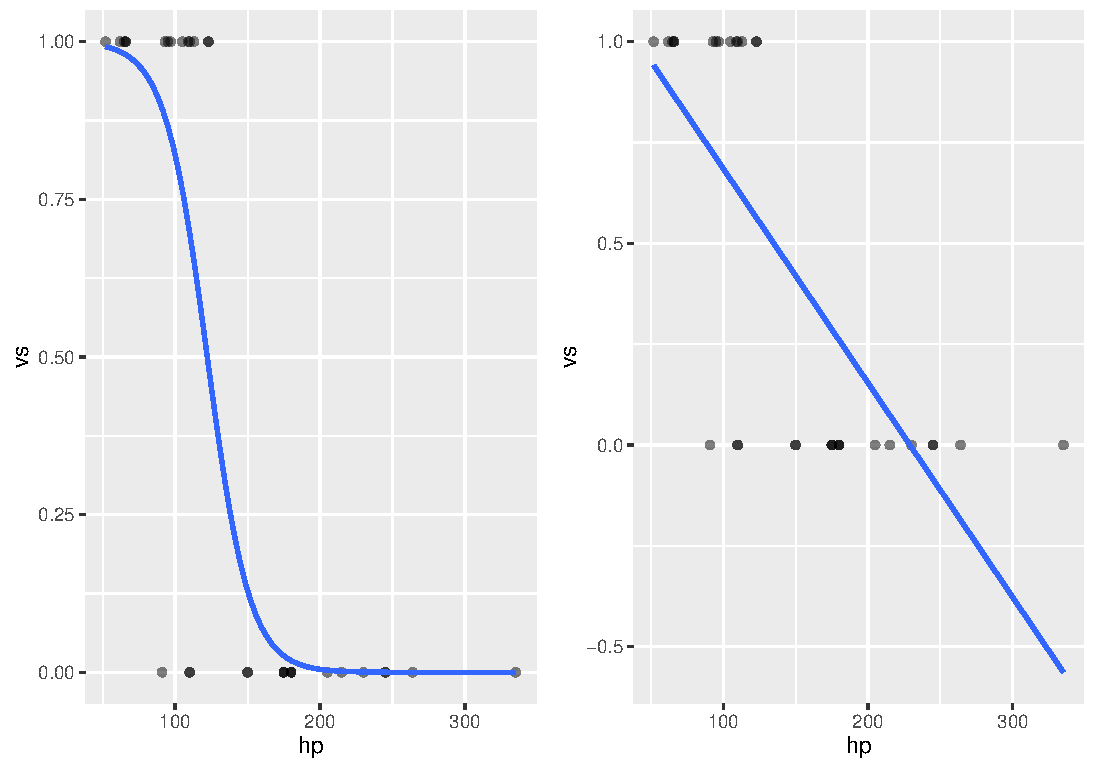
\includegraphics[width=0.75\textwidth]{figures/linear-vs-logistic-example.pdf}
    \caption[Linear versus binomial regression for a binary response.]{Illustrative example of fitting a linear model (to the right) versus a generalized (binomial) linear model (to the left) when the response is binary. The data used is from the standard \texttt{mtcars} set provided by R \autocite{r-core-team}. The response is the engine type (\texttt{vs}), either V-shaped or straight, and the covariate is gross horsepower (\texttt{hp}).}
    \label{fig:illustrative linear-binomial difference}
\end{figure}

Binomial regression is a generalized linear model (GLM). In GLMs, we assume that the response follows a distribution of the exponential family, such as the binomial, Poisson, exponential, or beta distribution. The expected value of the response links to a linear predictor $\bm\eta$ through a link function. More precisely, a GLM can be written as
\begin{equation}
g(\operatorname{E}[\bm Y | \bm X]) = g(\bm \mu) = \bm \eta = \bm X \bm \beta \ ,
\label{eq:glm definition}    
\end{equation}
where $g$ is the link function, $\bm\eta$ is the linear predictor, $\bm\mu$ is the expected value of the distribution of $\bm Y | \bm X$, and $\bm X$ and $\bm\beta$ are as previously defined. For the example of binary binomial regression, we get $\bm Y | \bm X \sim \operatorname{Bern}(\bm\mu)$, that is, $\bm Y | \bm X$ is assumed to have a Bernoulli distribution with mean $\bm\mu$. The common link functions for binomial regression are the logit, probit, and cloglog (complementary log-log) links, and are provided in \autoref{tab:link functions}.

Extending on the idea of an LMM, we have generalized linear mixed models (GLMMs) whose linear predictor $\bm\eta$ can include random effects, in addition to fixed effects. In general, a GLMM will have the form
\begin{align}
    \bm \eta &= \bm X\bm\beta + \bm U \bm \gamma \ , \nonumber \\
    \bm \mu &= g^{-1}(\bm\eta) \ ,  \\
    \bm Y | \bm X &\sim \mathcal D(\bm\mu, \bm\theta) \ , \nonumber
    \label{eq:general glmm}
\end{align}
for a distribution $\mathcal D$ of the exponential family with expected value $\bm\mu$ and (potentially additional) parameters $\bm\theta$.

\begin{table}
    \centering
    \begin{tabular}{ll}
    Link function     & Expression  \\ \midrule
    Logit   & $\log(y_i/(1-\log(y_i)))$ \\
    Probit  & $\Phi^{-1}(y_i)$ \\
    Cloglog & $\log(-\log(1-y_i))$
    \end{tabular}
    \caption[Link functions for binomial regression]{Most common link functions for binomial regression. Here, $\Phi$ is the cumulative density function of a standard normal distribution, $\mathcal N(0,1)$.}
    \label{tab:link functions}
\end{table}

\section{Models in quantitative genetics} 
\label{sec:theory:qg models}
We will use the animal model, which is a specific GLMM, to estimate the additive genetic variance. For context, we first introduce the infinitesimal and threshold model.

\subsection{The threshold model}
\label{sec:theory:threshold model}
The infinitesimal model in quantitative genetics assumes that any phenotypic trait is influenced by an infinite number of loci, all of which have some infinitesimal effect. In simpler terms, the trait of an offspring is Gaussian around the mean of its two parents with a variance independent of the values of the parents \autocite{barton2017}. The motivation behind this modeling choice dates back to \textcite{galton1886}, suggesting a law of ancestral heredity, where the phenotype is decided as the sum of geometrically declining contributions from parents and further up the pedigree. Each ancestor had a probability $p$ of passing the trait to the next generation. This idea is equivalent to the framework we use today, which is an additive genetic trait with the heritability concept replacing, and generalizing, the probability $p$ \autocite{bulmer1998}.

The infinitesimal model motivates us to use a normal distribution with a random effect. However, Gaussian models struggle to provide accurate predictions of binary phenotypes. To remedy this, the infinitesimal model can be extended to allow for more complex trait modeling, namely through the threshold model. Rather than trying to model a specific trait, we consider a latent trait, also called the liability, with a normal distribution. In the example of modeling a binary trait, for a given threshold $M$, the values attained below $M$ are cast to the one binary category, and all values above are set to the latter. \autoref{fig:theory:illustration-threshold} shows an illustration of the threshold model.
\begin{figure}
    \centering
    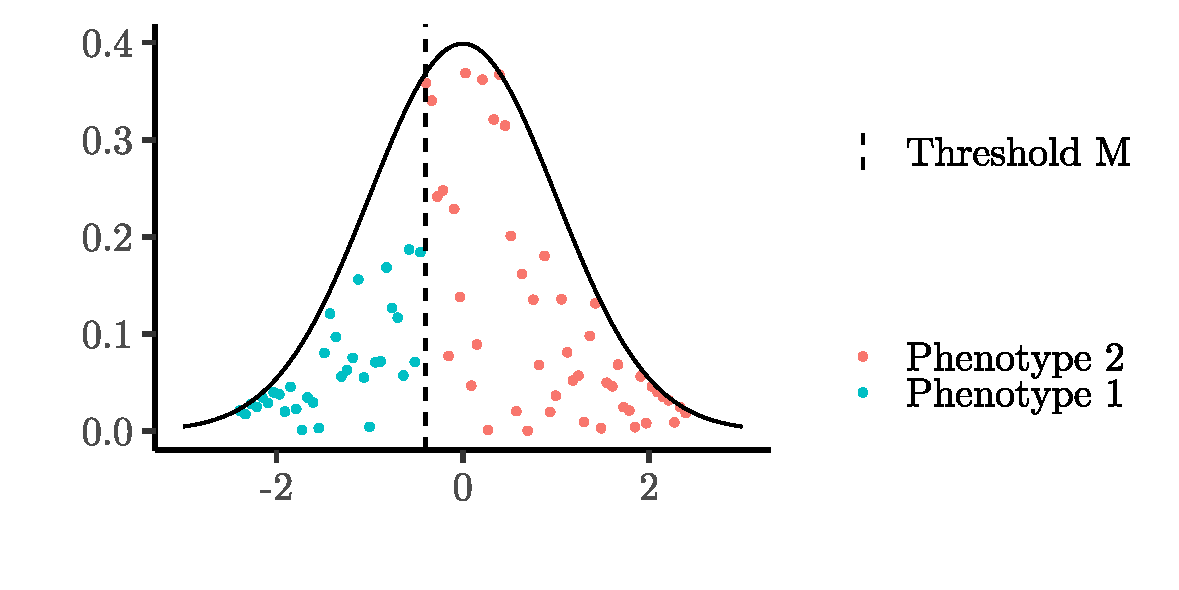
\includegraphics[width=0.75\textwidth]{figures/illustration_thresholdmodel.pdf}
    \caption[Illustration of the threshold model]{Illustration of the threshold model for a binary phenotypic trait. The blue points are realizations of the normal distribution less than the threshold value $M$ and thus belong to phenotype 1. Consequentially, the realizations above $M$ are the red points and belong to phenotype 2.}
    \label{fig:theory:illustration-threshold}
\end{figure}
The heritability computed from the liability trait can be transformed into an observation-scale heritability using the relation
\begin{equation}
h^2_{\text{liab}} = \frac{p(1-p)}{t^2}\;h^2_{\text{obs}} \ ,
\label{eq:heritability for threshold model}
\end{equation}
where $p$ is the proportion of one of the binary phenotypes in the population, and $t$ is density in $\mathcal N(0,1)$ at the $p$th quantile \autocite{dempster1950heritability, de2018quantitative}. The idea of the threshold model has been extended further into a multiple threshold model; see, for instance, \textcite{reich1972use}.

An important result is that \eqref{eq:heritability for threshold model} can be used for Gaussian models fitted to a binary trait when the binary trait is relatively well balanced \autocite{vanvleck1972, elston1977}. This result suggests that a linear (mixed) model can be sufficient to model binary traits if one scales the outcome by a scalar value dependent on the data. Note that \textcite{elston1977} mention that the variation in liability among groups (in terms of the response) should be small for the approximation to be valid. There is also little to no literature exploring the stability of the approximation when including fixed effects in the model.

\subsection{The animal model} \label{sec:theory:animal model}

The animal model is a mixed model that incorporates genetic information as a variance-covariance structure in a random effect. The model can use information from a complex pedigree encoded in a matrix, to estimate the causal components of the phenotypic variance \autocite{kruuk2004}. Whereas alternatives often must assume that there is no assortative mating, inbreeding, or selection, the animal model can account for all three. In a Gaussian case, the animal model can be expressed as the linear mixed model
\begin{align}
    \label{eq:animal model gaussian}
        \bm Y &= \bm X\bm\beta + \bm Z_a \bm a + \bm Z \bm u + \bm \varepsilon \ , \\
        \bm a &\sim \mathcal N(\bm 0,\bm A \sigma^2_A) \ , \nonumber \\
        \bm \varepsilon & \sim \mathcal N(\bm 0,\bm I \sigma^2_E) \ , \nonumber
\end{align}
where $\bm Y$ is the phenotypic trait of interest, $\bm a$ are called the breeding values, or the (total) additive genetic merit, and $\bm \varepsilon$ are the errors. Furthermore, $\bm X\bm \beta$ are the intercept and fixed effects, and each $\bm Z_j u_{ji}$ are the random effects other than the breeding values.

% \subsubsection{Additive genetic relationship matrix}
A key component of the animal model is the additive genetic relationship matrix $\bm A$.
Before defining $\bm A$, we define the coefficient of ancestry, $\Theta_{ij}$, to be the probability that an allele drawn from individual $i$ is the same as an allele from individual $j$. Then we have that $\Theta_{ii}$, that is, self-relatedness, is $\frac12$ and if $i$ and $j$ have a parent-offspring relationship, $\Theta_{ij}=\frac14$. We can then define $\bm A$ so that each $A_{ij} = 2\Theta_{ij}$.
In terms of notation, the total phenotypic variance on the observed scale will be written as $\sigma^2_P$, which is the sum of additive genetic variance, environmental and / or residual variance. Recall that heritability is the proportion of phenotypic variance explained by the additive genetic variance, which now can be expressed mathematically as
\begin{equation}
 h^2_\text{obs} = \frac{\sigma^2_A}{\sigma^2_P} \ .
\end{equation}


\subsection{The animal model for non-Gaussian traits}
\label{sec:theory:interpret heritability}
The threshold model has been used for binary and, in general, categorical traits.
One can show that there is an equivalence between a binomial GLMM whose link function is the probit link, and the threshold model \autocite{de2016general}.
With the extensions to GLMMs, we also have a broader framework that can accurately model non-Gaussian traits.

Specifically, we use a GLMM such as a binomial model with a probit link for the case of a binary trait. Although a probit-based animal model has a better predictive power than a Gaussian animal model, the nonlinearity of the link functions confounds the actual biological values of interest. To illustrate the scales more clearly, we consider a simple binomial probit animal model by
\begin{align}
\label{eq:theory:binom AM latent}
    \bm \eta = \beta_0 + \bm a \ ,  \\
    \bm a \sim \mathcal N(\bm 0, \bm A \sigma^2_A) \ ,\\
    \bm \mu = \Phi(\bm \eta) \ ,\\
    \bm Y | \bm X \sim \operatorname{Bern}(\bm \mu) \ . 
\end{align}
The estimated variance components $\hat\sigma^2_A$ in the model are on the same scale as \eqref{eq:theory:binom AM latent}, namely the latent scale, meaning that the variance is additive on the linear predictor's scale. However, it is no longer additive in relation to observed values, which follow a Bernoulli distribution whose mean is linked through the nonlinear function $\Phi$, that is, the cumulative density function for $\mathcal N(0,1)$. We also illustrate this concept in \autoref{fig:theory:illustration-probit-fitted-values}, where the posterior latent fitted values are shown with the true observations. While the fitted values on the latent scale are far from the true observations, passing the inverse of the link function will obtain the \textit{expected} scale, which reflects the phenotypic mean. However, as apparent in the same figure, none of these scales is the same as the observed data, which are binary realizations of a Bernoulli distribution. In summary, since the link function $g$ is nonlinear, we get a non-additive genetic variance.

\begin{figure}
    \centering
    \begin{subfigure}{0.8\textwidth}
    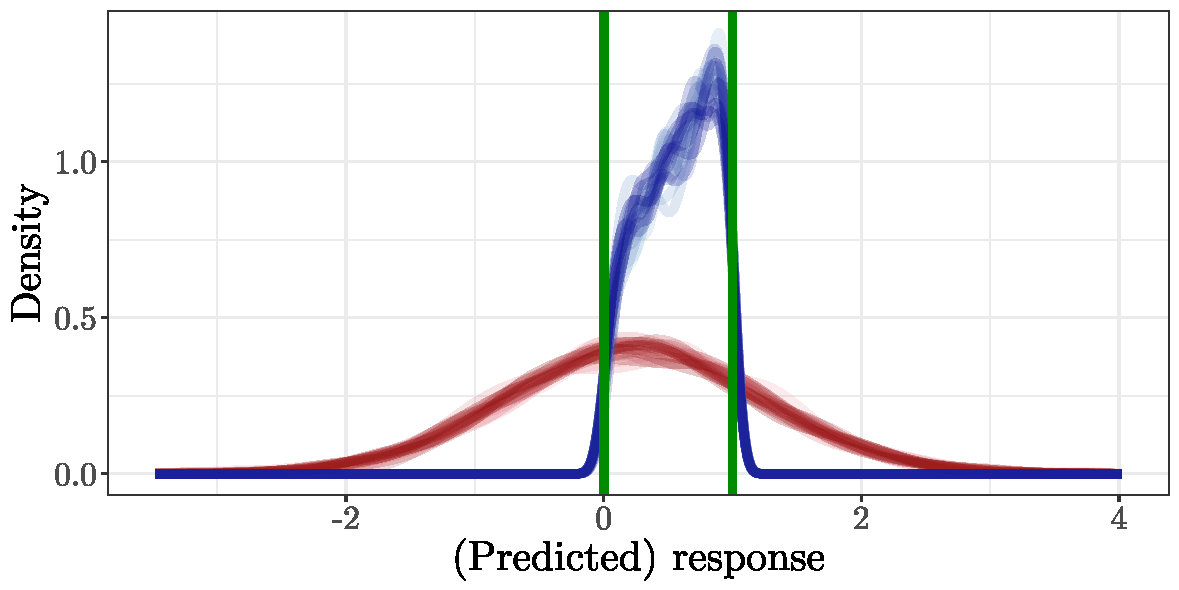
\includegraphics[width=\textwidth]{figures/illustration_probit_scales_fitted_values.pdf}
    \end{subfigure}
    \begin{subfigure}[b]{0.4\textwidth}
        
\includegraphics[width=\textwidth]{figures/illustration_probit_scales_fitted_values_legend.pdf}
    \end{subfigure}
    \caption[Illustration of fitted values for a probit animal model]{Illustrative figure showing the fitted values obtained in a binomial probit model. The red lines, $\eta\in(-\infty, \infty)$, are the marginal fitted values, i.e., the fitted values on the latent scale. By using the inverse of the link function, we obtain the dark blue estimate $\Phi(\eta)\in(0,1)$, which can be interpreted as the expected scale. Lastly, the green lines show the true observations $y\in\{0,1\}$. The estimates ($\eta$ and $\Phi(\eta)$) show $20$ posterior samples of these estimates, hence their blurry shape compared to the true observations.} \label{fig:theory:illustration-probit-fitted-values}
\end{figure}

We have motivated the interest in applying animal models %in wild populations
to get heritability estimates. However, only reporting the heritability on the latent scale is not viable, as inferring parameters on the observation scale should be the standard approach \autocite{de2018quantitative}. This raises the issue of how one can get usable estimates on the original observation scale when using nonlinear models.
There are several potential remedies to obtain an estimate comparable to the observation scale, one of them by introducing \textit{ link variance}. By sending the linear predictor through the nonlinear inverse link function $g^{-1}(\eta_i)$, one introduces variance. Traditionally, this is captured by adding a term to the denominator in the heritability estimate, for instance in the probit case
\begin{equation}
    h^2_{\Phi} = \frac{\sigma^2_A}{\sum_i \sigma^2_i +1} \ ,
    \label{eq:link variance h2 phi}
\end{equation}
where $\sum_i \sigma^2_i$ is the sum of the variance components from the random effects. Including the term $1$ in the denominator captures the link variance for a probit model and attains the same scale as would be achieved using the threshold model, that is, the \textit{liability scale}. Similarly, the link variance in a binomial model with a logit link is $\pi^2/3$ and the cloglog link is $\pi^2/6$ \autocite{nakagawa2017}. Although this method is easy to use, it does not address the issue of fixed effects influencing heritability and does not yield heritability estimates on an observation scale.

In wild populations, we must interpret heritability as conditioned on any fixed effects chosen in the model \autocite{wilson2008}. To remedy this, \textcite{de2016general} introduces a method that attempts to obtain heritability estimates on the observation scale by averaging over fixed effects. The algorithm is based on the same three hierarchical scales introduced by \autoref{fig:theory:illustration-probit-fitted-values}, namely, the latent scale, the expected scale and the observation scale.
%The latent scale is the direct output of the model, for instance, the $\bm\hat\beta$ or the variance components $\hat\sigma^2_A$ and $\hat\sigma^2_E$. The expected scale is simply the inverse link function applied to the parameters on the latent scale. Thus, the observation scale consists of realizations from the assumed distribution given the expected values defined from the expected scale and potentially other parameters (such as variance).
The primary goal will be to convert from the latent scale to the observation scale, as presented below. 

\subsubsection*{A general back-transformation algorithm}
\textcite{de2016general} also suggests general formulae, both tackling the back-transformation of variables onto the observation scale and providing a method to average over the fixed effects. The purpose of averaging over fixed effects is to attempt to remove the heritability's dependence on model choices of fixed effects. 

The algorithm is detailed in \autoref{alg:qgglmm}. In the algorithm, $g^{-1}$ is the inverse link function for a given model, $\sigma^2_{RE}$ is the sum of variance from all random effects, $f_{\mathcal{N}}(x;\mu,\sigma^2)$ is the density function for the distribution $\mathcal{N}(\mu,\sigma^2)$, and $\mathcal{V}$ is a distribution-specific variance function. 


\begin{algorithm}
\caption{General method for observation-scale heritability $h^2_\Psi$.} \label{alg:qgglmm}
    \begin{algorithmic}
    \State \textbf{Input:} Latent additive genetic variance $\sigma^2_{A,l}$ and total phenotypic variance $\sigma^2_{RE,l}$, either intercept $\mu$ or \texttt{predict} (latent marginal estimates). Optional: $w$, width for integration.
    \If{\texttt{predict} given but not $\mu$}
        \State $\Tilde{\bm\mu} \gets$ \texttt{predict}
    \Else
        \State $\Tilde{\bm\mu} \gets [\mu, \dots, \mu]^\top$ \algorithmiccomment{Such that $\Tilde{\bm\mu} = [\Tilde{\mu}^{(1)}, \dots, \Tilde{\mu}^{(N)}]^\top$}
    \EndIf
    \State $\bar z \gets \frac1N\sum_{i=1}^N \int_{\tilde\mu^{(i)} - w \sqrt{\sigma^2_{RE,l}}}^{\tilde\mu^{(i)} + w \sqrt{\sigma^2_{RE,l}}} g^{-1}(x)f_{\mathcal N}(x; \mu=\tilde\mu^{(i)},\sigma^2=\sigma^2_{RE,l})dx$
    \State $\sigma^2_{RE, exp} \gets \left(\frac1N\sum_{i=1}^N \int_{\tilde\mu^{(i)} - w \sqrt{\sigma^2_{RE,l}}}^{\tilde\mu^{(i)} + w \sqrt{\sigma^2_{RE,l}}} \left(g^{-1}(x)\right)^2 f_{\mathcal N}(x; \mu=\tilde\mu^{(i)},\sigma^2=\sigma^2_{RE,l})dx\right)-\bar z^2$
    \State $\sigma^2_{RE, dist} \gets \frac1N\sum_{i=1}^N \int_{\tilde\mu^{(i)} - w \sqrt{\sigma^2_{RE,l}}}^{\tilde\mu^{(i)} + w \sqrt{\sigma^2_{RE,l}}} \mathcal{V}(x) f_{\mathcal N}(x; \mu=\tilde\mu^{(i)},\sigma^2=\sigma^2_{RE,l})dx$
    \State $\sigma^2_{RE,obs} \gets \sigma^2_{RE, exp} + \sigma^2_{RE, dist}$
    \State $\Psi \gets \frac1N\sum_{i=1}^N \int_{\tilde\mu^{(i)} - w \sqrt{\sigma^2_{RE,l}}}^{\tilde\mu^{(i)} + w \sqrt{\sigma^2_{RE,l}}} \frac{\partial g^{-1}(x)}{\partial x} f_{\mathcal N}(x; \mu=\tilde\mu^{(i)},\sigma^2=\sigma^2_{RE,l})dx$
    \State $h^2_{\Psi} \gets \frac{\Psi^2 \sigma^2_{A,l}}{\sigma^2_{RE,obs}}$
    \State \textbf{Returns: } $h^2_{\Psi}$
    \end{algorithmic}
\end{algorithm}

In the case where we have a binomial probit model, the sequence obtains a closed-form solution, given by \autoref{alg:qgglmm-probit}, and will be significantly faster than, for instance, a binomial logit model.

\begin{algorithm}
\caption{Observation-scale heritability for a binomial probit model.} \label{alg:qgglmm-probit}
    \begin{algorithmic}
    \State \textbf{Input:} Latent additive genetic variance $\sigma^2_{A,l}$ and total phenotypic variance $\sigma^2_{RE,l}$, either intercept $\mu$ or \texttt{predict} (latent marginal estimates).
    \If{\texttt{predict} given but not $\mu$}
        \State $\Tilde{\bm\mu} \gets$ \texttt{predict}
    \Else
        \State $\Tilde{\bm\mu} \gets [\mu, \dots, \mu]^\top$ \algorithmiccomment{Such that $\Tilde{\bm\mu} = [\Tilde{\mu}^{(1)}, \dots, \Tilde{\mu}^{(N)}]^\top$}
    \EndIf
    \State $p \gets \frac{1}{N} \sum_{i=1}^N 1-\Phi(0;\mu=\tilde\mu^{(i)},\sigma^2=\sigma^2_{RE,l}+1)$
    \State $\sigma^2_{RE,obs} \gets p(1-p)$
    \State $\Psi \gets \frac{1}{N}\sum_{i=1}^N f_{\mathcal N}(0;\mu=\tilde\mu^{(i)},\sigma^2=\sigma^2_{RE,l}+1)$
    \State $h^2_{\Psi} \gets \frac{\Psi^2 \sigma^2_{A,l}}{\sigma^2_{RE,obs}}$
    \State \textbf{Returns: } $h^2_{\Psi}$
    \end{algorithmic}
\end{algorithm}

\section{Bayesian inference and INLA}

\subsection{The Bayesian statistical modeling framework}

We can consider two main frameworks for statistical modeling: a frequentist approach and a Bayesian approach. When modeling with a frequentist approach, we assume that the parameters in a model have one true value, whereas, in a Bayesian approach, we interpret them as stochastic with their own distributions. The prior distribution in the Bayesian framework represents the knowledge that we have in the model before we observe the data itself. Using an appropriate prior can improve the accuracy of the model. Another key component in Bayesian statistics is that the methods used provide a probabilistic interpretation of the fitted values, which is helpful for further inference in the model of interest. In terms of notation, we define the operator $\operatorname{MAP}[\bm X]$ as the maximum a posteriori of a random variable $\bm X$ with a posterior distribution and represents the mode of the posterior distribution computed for $\bm X$.
Simulation studies have also shown that in the case of the estimation of heritability of binary traits, the use of Bayesian models is the most effective \autocite{devillemereuil2013}, further motivating the use of Bayesian frameworks.

\subsubsection*{Penalized complexity priors}

A suitable choice of priors can significantly improve the performance of a model, while choosing unsuitable priors can increase the bias in the model. Thus, choosing prior distributions in a Bayesian model is not a trivial task. When there is little prior knowledge, noninformative priors, and improper priors (such as the uniform distribution) can be used. An improper prior is any prior distribution that integrates to a non-finite value. However, improper priors can also lead to other issues, such as improper posterior distributions. 

For this thesis, we will be using penalized complexity (PC) priors \autocite{simpson-pcpriors}. By introducing penalized complexity priors, simpler and more interpretable models will be prioritized, while more complex models that tend to overfit the data will be penalized. PC priors require only two parameters, namely $U$ and $\alpha$ where $0<\alpha<1$. Informally, the prior $\operatorname{PC}(U, \alpha)$ on some parameter $\bm\theta$ is expressed so that the probability $\operatorname{Pr}(\bm\theta \le U) = 1-\alpha$.

For the case of a random effect $[a_1, \dots, a_n]^\top = \bm a \sim \mathcal N(\bm 0, \bm A \sigma^2_A) = \mathcal{N}(\bm 0,\bm A \tau_A^{-1})$, the PC prior becomes a type-2 Gumbel distribution with respect to $\lambda$,
\begin{equation}
    \pi(\tau_A) = \frac{\lambda}{2} \tau^{-3/2} \exp(-\lambda\tau_A^{-1/2}),\quad \tau_A>0,\; \lambda>0 \ ,
\end{equation}
and with $\operatorname{Pr}(\tau_A^{-1/2} \le U)=1-\alpha$, we obtain $\lambda=-\ln(\alpha)/U$ \autocite{simpson-pcpriors}. PC priors have a parameterization so that $U$ resembles the standard deviation, for example, a PC prior $\operatorname{PC}(1,0.05)$ for the breeding values $\bm a$ would resemble $\operatorname{Pr}(\sigma_A \le 1) = 0.95$.

\subsection{The INLA computing scheme}
INLA is an abbreviation for the term integrated nested Laplace approximation and is an alternative to fitting Bayesian models using Markov chain Monte Carlo (MCMC). INLA is a faster alternative to obtain posterior distributions for latent Gaussian models. In this brief review of INLA, we use the notation and definitions provided in \textcite{inla-lecturenotes}.

A latent Gaussian model is a relatively broad class of models consisting of observations $\bm y$, a latent field $\bm x$, and hyperparameters $\bm \theta$ with a partition $\bm\theta = (\bm \theta_1, \bm \theta_2)^\top$. We have that

\begin{align}
    \bm y | \bm x \sim \prod_i \pi(y_i | x_i, \dots, \bm \theta_1) \label{eq:inla:lgm1} \\
    \bm x | \bm \theta_1 \sim \mathcal N(0, \bm Q(\bm\theta_2)^{-1}), \label{eq:inla:lgm2} \ ,
\end{align}
where \eqref{eq:inla:lgm1} implies that $\bm y$ is conditionally independent given $\bm x$ and $\bm \theta_1$ and $\pi(\cdot)$ indicates the distribution of a random variable, and $\bm Q$ in \eqref{eq:inla:lgm2} is the precision matrix for the latent field $\bm x$. Furthermore, we assume that $\bm x$ is a Gaussian Markov Random Field (GMRF). To obtain effective computations within the INLA framework, the precision matrix $\bm Q$ should be sparse. Within the context of the animal model, $\bm Q = \bm A^{-1}$, which has been shown to be sparse \autocite{steinsland2010utilizing}. The linear predictor in a latent Gaussian model is

\begin{equation}
    \eta_i = \alpha + \sum_{l} f_i(u_{l,i}) + \sum_k \beta_k z_{k,i} + \varepsilon_i \ ,
\end{equation}
which we can use to express both linear models, GLMs, GLMMs, and more complex models like geostatistical models. 

\subsubsection*{The INLA computing scheme} 

The first step of the INLA computing scheme is to obtain estimates for the marginal hyperparameter distribution. That is, $\pi(\bm\theta_j | \bm y) = \int \pi(\bm \theta | \bm y) d\bm\theta_{-j}$, which we compute numerically. The notation $\bm\theta_{-j}$ means all elements of $\bm\theta$ except $j$. In particular, we can approximate the marginal hyperparameter distribution using the expanded form \autocite{gentleINLA}
\begin{equation}
    \pi(\bm\theta|\bm y) \approx \left.\frac{\pi(\bm y | \bm x, \bm \theta) \times \pi(\bm x | \bm \theta) \times \pi(\bm \theta)}{\Tilde{\pi}_G(\bm x | \bm \theta, \bm y)}\right|_{\bm x = \operatorname{MAP}[\pi(\bm x |\bm \theta, \bm y)]} \ ,
\end{equation}
where $\Tilde{\pi}_G$ is the GMRF approximation.
With these, INLA selects suitable support points (for non-scalar $\bm\theta$) with Newton-like numerical methods such that each $\bm\theta_k$ has weight $\Delta_k$ \autocite{gentleINLA}.

With the marginal hyperpriors, we can get the distribution of the latent space by $\pi(x_i | \bm y)=\int \pi(x_i|\bm\theta,\bm y)\times\pi(\bm\theta|\bm y)d\bm\theta$ with additional Laplace approximations, given that they are not Gaussian. The Laplace approximation can be done using either a full Laplace approximation or a simplified version based on a skew-normal distribution to a series expansion of $\Tilde{\pi}(x_i|\bm\theta, \bm y)$ \autocite{inla-lecturenotes}.
Lastly, we can obtain the posterior estimate $\tilde{\pi}(x_i | \bm y)$ as
\begin{equation}
    \Tilde{\pi}(x_i | \bm y) = \sum_k
    \Tilde{\pi}(x_i | \bm \theta_k, \bm y) \times \tilde{\pi}(\bm\theta_k|\bm y) \times \Delta_k \ .
\end{equation}
The package R-INLA \autocite{inla2009} implements the computing scheme and will be used to fit all models in this thesis.


% \section{Notation}
% Placeholder in case I need to define new notation...

\chapter{Methods}

\section{Overview}
In this chapter, we will present the methods and model specifications used to answer the research question. We will also introduce the simulation and application data used in the study. Supplementary to the chapter is the complete R code provided in \autoref{app:Rmd script}.

The initial segment of the thesis will investigate different scales of heritability, with particular attention given to the threshold model. In the threshold model, we assume that the underlying scale is a Gaussian distribution. This distribution is not available in application contexts. However, by using simulations, we can construct this Gaussian linear predictor and produce a corresponding binary response variable using a dichotomization of the linear predictor. Then, by computing the heritability from a Gaussian model fitted with the dichotomized response, we can scale it onto the liability scale with the coefficient $p(1-p)/t^2$ from the threshold model \eqref{eq:heritability for threshold model}, and compare the model's performance to the true underlying distribution. If the results from the Gaussian model coincide well with the true heritability, we would strengthen the claim that Gaussian modeling may be sufficient to accurately estimate heritability.

The second segment of the thesis aims to compare heritability from state-of-the-art back-transformation strategies applied to a probit model, with heritability from our Gaussian mixed model. The main focus will be to compare the posterior heritability density in the Gaussian and probit models, where the probit model attains the same scale as the Gaussian using back-transformations, namely the observation scale. If the Gaussian observation-scale heritability is similar to that of the more complex back-transformation algorithms, one may conclude that linear mixed models can be sufficient when primarily interested in the additive genetic variance (or heritability) on the observation scale. These comparisons will be the most important results when discussing a Gaussian model's performance on binary traits.

\section{Statistical models}
% Include Gaussian, probit models and all state-of-the-art methods
We define the general statistical models and heritability scales used throughout the thesis in this section. Methods specific to the simulation or application data are provided in the following sections.
%Furthermore, having a method for simulating data can provide more generality for the other areas of research in this thesis. % This sentence doesn't belong since this is a general section and not about motivating simulation.

% \subsection{Gaussian and binomial model}
% We highlight the statistical models used for all datasets in this section, and introduce methods specific to the application and simulation data in the sections.
In general, the Gaussian model is on the form
\begin{equation}
    \bm y = \beta_0 + \sum_{i=1}^n \beta_i \bm x_{i} + \sum_{j=1}^m \gamma_{0,j} \bm z_{j} + \bm a + \bm\varepsilon \ ,
    \label{eq:method:general gaussian model}
\end{equation}
where $\bm y$ is the response, $\beta_0$ is the intercept, $\beta_i \bm x_i$ are the $n$ fixed effects, $\gamma_{0,j}\bm z_j$ are the random effects, $\bm a \sim \mathcal N(\bm 0, \bm A \sigma^2_A)$ are the breeding values for a defined relatedness matrix $\bm A$, and $\bm\varepsilon \sim \mathcal N(\bm 0, \bm I \sigma^2_E)$ is the error term. The corresponding binomial probit model is defined as
\begin{align}
    \label{eq:method:general probit model}
    \bm \eta = \beta_0 + \sum_{i=1}^n \beta_i \bm x_{i} + \sum_{j=1}^m \gamma_{0,j} \bm z_{j} + \bm a \ , \\
    \E{\bm y | \bm X} = \Phi(\bm \eta) \ ,
\end{align}
where $\Phi$ is the cumulative density function of $\mathcal N(0,1)$. Moreover, all random effects are given a penalized complexity prior (PC prior) of the form $\operatorname{PC}(U, \alpha=0.05)$ \autocite{simpson-pcpriors}. Note that PC priors are parameterized so that $U$ denotes the standard deviation and not the variance \autocite{inla2009}. The value of $U$ in the PC priors, as well as the specific fixed and random effects, are denoted in the subsequent sections regarding the application and simulation data, respectively.
Since we are using a Bayesian statistical framework, we can get a posterior distribution of the random effects estimates and hence a posterior of the estimated heritability. We use the INLA framework \autocite{inla2009} for Bayesian inference and model fitting.

\subsection{Comparing with state-of-the-art techniques}
\label{sec:method:compute h2}
Initially, we fit both a Gaussian and a binomial probit model to the datasets. With the fit of the models, we can compute the heritability. For the Gaussian models, this will simply be
\begin{equation}
\label{eq:heriability directly computed}
    h^2_\text{obs} = \frac{\hat \sigma^2_A}{\hat \sigma^2_P}=\frac{\hat{\sigma}^2_A}{\hat\sigma^2_A + \hat\sigma^2_E + \sum_{j} \widehat{\operatorname{Var}[\gamma_{0,j}]}} \ ,
\end{equation}
where $\sum_j \widehat{\Var{\gamma_{0,j}}}$ is the sum of variances from all $j$ random effects, excluding the breeding values whose variance is $\hat\sigma^2_A$.
% \begin{equation}
%     h^2_{obs} = \begin{cases}
%         \frac{\hat\sigma^2_A}{\hat\sigma^2_A+\hat\tau_{0,1}+\hat\tau_{0,2}} &\text{for application data} \\
%         \frac{\hat\sigma^2_A}{\hat{\sigma^2_A}+\widehat{\operatorname{Var}[\varepsilon]}}  &\text{for simulation data}.
%     \end{cases}
% \end{equation}
The observation-scale heritability is thus directly computable from the estimated variance components without transformation. However, computing heritability for a probit model \eqref{eq:method:general probit model} would yield a latent scale estimate of heritability, denoted as $h^2_\text{lat}$. To obtain a comparable estimate to $h^2_\text{obs}$, it is necessary to use some of the techniques described in the theory chapter. 
Once the estimates are computed for the different scales, we can compare their posterior distributions to infer conclusions about how well the Gaussian model performs. The resulting heritability scales are described in \autoref{tab:h2 notation}. In particular, we want to compare $h^2_\text{obs}$ with $h^2_\Psi$ and $h^2_\text{liab}$ with $h^2_{\Phi}$.
% \begin{table}[b]
% \centering
% \begin{tabular}{@{}lllll@{}}
% \toprule
%                 & \multicolumn{2}{c}{Gaussian model} & \multicolumn{2}{c}{Probit model} \\ \midrule
%                 & Notation          & Expression      & Notation        & Expression     \\
% Observation scale      & $h^2_{\text{obs}}$ & \eqref{eq:heriability directly computed}  & $h^2_\Psi$ & Alg. \ref{alg:qgglmm-probit}  \\
% Liability scale & $h^2_\text{liab}$  & \eqref{eq:heritability for threshold model}   & $h^2_\Phi$ & \eqref{eq:link variance h2 phi}  \\
% Latent scale    &                   &                 & $h^2_\text{lat}$     & \eqref{eq:heriability directly computed}          \\ \bottomrule
% \end{tabular}
% \caption[Heritability notation for different scales]{The notation used throughout the other sections for the different scales and models. The subsets "obs" and $\Psi$ and $\Phi$ will be in the observation scale, those with "liab" and $\Phi$ are on a liability scale, and "lat" indicates the latent scale. The estimates on the same scales will be subject to comparison, i.e., $h^2_\text{obs}$ with $h^2_\Psi$ and $h^2_\text{liab}$ with $h^2_\Phi$, respectively. The "Expression" column provides a reference describing how to transform onto the said scale.}
% \label{tab:heritability notation}
% \end{table}

\subsubsection{Observation scale heritability from probit model} \label{sec:method:qgglmm settings}
When estimating the heritability from a probit model on the observation scale, i.e., $h^2_{\Psi}$, we can choose to work with the mode $\operatorname{MAP}[\bm\mu]$ of the intercept estimate $\bm\mu$, or using the latent marginal estimates. By simply using the intercept, we do not average over fixed effects, which could lead to significantly different results \autocite{de2016general}, and is denoted in the results as \textit{No averaging}. In particular, when not averaging over fixed effects, the algorithm simplifies to
\begin{align}
    p = 1 - \Phi(0; \operatorname{MAP}[\bm\mu]; \hat\sigma^2_{RE}+1) \ , \\
    h^2_\Psi = \frac{f_\mathcal{N}(0; \operatorname{MAP}[\bm\mu], \hat\sigma^2_{RE}+1)\; \hat\sigma^2_A}{p(1-p)} \ ,
\end{align}
where $p$ is the observation-scale estimated phenotypic mean. Using latent marginal estimates, which is $\bm X\bm\hat{\bm\beta}$ marginal to random effects, we also have two options, denoted by \textit{Frequentist} or \textit{Bayesian}. The frequentist approach is to use $\operatorname{MAP}[\bm X\bm\hat{\bm\beta}]$ for each predictor so that each sample of $h^2_{\Psi}$ achieves the same predicted values. For example, by sampling 1000 times for a dataset with 500 observations, the same 500 predictors would be used for all 1000 samples. The other option is more in line with the Bayesian framework, in which we draw one sample from the posterior of each $\bm X \bm{\hat\beta}$ as many times as the sampling number for $h^2_{\Psi}$, but is also slower. Although this method is slower, it is theoretically more sound, given that we use a sufficiently large sample size. Using samples instead of the mode introduces more information, thus improving the estimate of posterior heritability. Comparing how the posteriors differ with these different approaches is relevant for understanding when they may be approximated with a Gaussian model.


\section{Simulation setup}
We lay out how we produce the simulated pedigree data and binary traits below. In short, we simulate a pedigree and binary response, from which we can fit a Gaussian model and scale the observation-scale estimated heritability back onto the liability scale.
% If the formula in the threshold model is reliable, we will expect the threshold-scaled estimated heritability to be close to that of the true value.

\subsection{Simulating a pedigree}
To make a proper model for the animal model, we need to make a simulated relatedness matrix $\bm A$, which requires a pedigree. We can generate a simulated pedigree using the R package \texttt{GeneticsPed} \autocite{geneticsPed}.
We use the ratio $N_e/N_c$ to determine the number of dams and sires, where $N_e$ is the effective population size and $N_c$ is the census population size. $N_e$ determines the biological rates such as genetic drift, and analyzing the ratio enables us to examine the impact of different traits and factors' influence on the effective population size \autocite{NeNc2002}. For the purposes of this simulation, we fix $N_e/N_c$ to $\frac12$ and generate $100$ individuals with $100\ N_e/N_c$ dams and sires, respectively, for $9$ generations providing $900$ data points. We also fix the additive genetic variance $\sigma_A^2$ for each simulation run. This is sufficient for generating a simulated pedigree and hence a relatedness matrix. Using the relatedness matrix, we may generate random deviates of breeding values $a_i$ of $\bm a=[a_1, \dots, a_n]^\top$ with $\bm a \sim \mathcal N(\bm 0, \bm A \sigma^2_A)$. With our setup, we require a technical modification of the methods \texttt{rbv()} from the R package \texttt{MCMCglmm} \autocite{mcmcglmm}, see \autoref{app:rbv-patch} for more details. The resulting pedigree also provides the generation number and sex for each individual, the latter of which can be used for the simulation of fixed-effects models.

With the defined pedigree and breeding values, we let $\Tilde{\bm \eta}$ be the linear predictor, for instance
\begin{equation}
    \Tilde{\bm\eta} = \bm a + \bm\varepsilon \ ,
    \label{eq:simulation linear predictor}
\end{equation}
where $\bm\varepsilon \sim \mathcal N(\bm 0,\bm I \sigma^2_E)$. In most cases, $\sigma^2_A$ defaults to the arbitrarily chosen value $0.5$ and $\sigma^2_E$ to $1$, unless otherwise stated. The linear predictor is the true, underlying normal distribution for the simulation.

\subsubsection{Simulating a binary response}

We can use the dichotomization of $\Tilde{\bm\eta}$ to define the simulated response variable as
\begin{equation}
y_i = \begin{cases}
0, \quad \eta_i\le c,\\
1, \quad \eta_i > c \ ,
\end{cases}
\label{eq:dichotomize round}
\end{equation}
for a cutoff value $c$ for each $\eta_i \in \Tilde{\bm \eta}$, hereby denoted as thresholding dichotomization. When $\Tilde{\bm \eta}$ is centered around zero, this dichotomization leads to a balanced phenotypic response ($p\approx 0.5$) with $c=0$. Alternatively, we can generate the responses $y_i$ as binomial realizations. Here, the probability of success $p_i$ is based on $\Tilde{\bm \eta}$ scaled between 0 to 1, that is,
\begin{equation}
     y_i \sim \operatorname{Bern}(p_i=\Phi(\eta_i)) \ .
     \label{eq:dichotomize binom}
\end{equation}
We also define $\hat p$ as the estimator to the marginal phenotypic mean, i.e., 
\begin{equation}
    \hat p = \frac{\sum_{i=1}^N\mathbbm{1}[y_i=1]}{N} \ .
\end{equation}
This is the same as $p$ used for the threshold model \eqref{eq:heritability for threshold model}, and we use the estimator for such computations.

\subsubsection{Fitting the model}
When fitting the model, we primarily include no fixed effects or any random effects other than the breeding value, and an iid random effect in the probit models. That is, $\bm y = \bm \beta_0 + \bm a + \bm\varepsilon$ in the Gaussian case and $\bm\eta = \beta_0+\bm a + \bm \gamma_0$ and $\bm\gamma_0\sim\mathcal N(\bm 0, \bm I)$. When it comes to the prior choice, we will use penalized complexity priors PC$(U, 0.05)$, where $U$ is rounded up to the closest order of magnitude when $\sigma^2_A \ge 1$. For example, if $\sigma_A$ is $3\cdot 10^2$, $U$ becomes $10^3$, meaning that we assume $\operatorname{Pr}(\sigma_A \le 10^3) = 0.95$. For $\sigma^2_A < 1$, the prior defaults to PC$(1,0.05)$. 


\subsection{Robustness tests}
\label{sec:method:robustness}
To properly evaluate the robustness of our techniques, we will look into alternative models using fixed effects and overdispersion, respectively. For the case of fixed effects, we generate simulation data using the linear predictor
\begin{equation}
\Tilde{\bm \eta} = \bm a + \beta_\text{sex} \bm x_{\text{sex}} + \bm \varepsilon \ ,
\end{equation}
where $\bm a$ and $\bm \varepsilon$ are as in \eqref{eq:simulation linear predictor}, $\bm x_{\text{sex}}$ are realizations of the individual's sex from the generated pedigree, and for a specified choice of $\beta_\text{sex}$. For a sufficiently large weighting of $\beta_\text{sex}$ compared to $\sigma^2_A$ and $\sigma^2_E$ and a fixed variance of $\bm x_\text{sex}$, we expect the variance in the fixed effect to dominate the linear predictor. Hence, we must include the fixed effect variances for heritability estimation for such models by adding the term $\beta_\text{sex}^2 \sigma^2_{\text{sex}}$, where $\sigma^2_{\text{sex}}$ is the unbiased sample variance of the observations for the \textit{sex} covariate, to the total phenotypic variance \autocite{nakagawa2013general}. The underlying heritability in the simulation becomes
\begin{equation}
    h^2_\text{liab} = \frac{\sigma^2_A}{\sigma^2_A+1+\bm\beta^2_\text{sex}\sigma^2_{\text{sex}}} \ .
\end{equation}

Another consequence of including a fixed effect is that $\eta$ will no longer necessarily be centered around zero. Thus, we define the cutoff point in the threshold-based dichotomization based on the quantiles of the simulated $\Tilde{\bm\eta}$. In particular, we will investigate the performance of the Gaussian model with a balanced $p\approx 0.5$ and an unbalanced phenotypic mean $p\approx 0.1$. In the runs where $p$ is imposed balanced, the cutoff is set to $\E{\Tilde{\bm\eta}}$, and in the unbalanced case, the cutoff is at the $(1-p)$th quantile. For simplicity, all runs use thresholding dichotomization.
We test the models with the presence of fixed effects with $\beta_\text{sex} = 10$ and $\beta_\text{sex}=100$. The variance explained by the fixed effect is $\beta_\text{sex}^2\sigma^2_\text{sex}=\beta_\text{sex}^2 p(1-p)$, for example $25$ for a balanced phenotypic mean ($p \approx 0.5)$ and $\beta_\text{sex}=10$.
For the case of overdispersion, we can change $\bm\varepsilon$ in the linear predictor for the simulation, so that $\bm\varepsilon \sim \mathcal{N}(\bm 0, \bm I \sigma^2_E)$ with a chosen $\sigma^2_E > 1$. In addition, we fit two probit models, one without the random iid effect $\bm\gamma_0$, and one model with the effect.

\section{Data description}
For the purposes of this thesis, the application dataset consists of observations of song sparrows from Mandarte Island. Researchers have collected data from this population since 1975, but we mainly use data from 1993-2018, as the individuals in these years have a complete pedigree \autocite{reid2021}. Song sparrows are socially monogamous and open nesting, but are known to aggressively defend territory against intrusion from neighboring males \autocite{reid2021, OLoghlen1999}.

The dataset contains parental linkage information for the individuals. In the pruned dataset, that is, observations between 1994 and 2018, we have 2722 individuals with a complete pedigree. In addition to parental knowledge, the data includes the natal year, brood date, sex, coefficients of inbreeding, and proportion of genetic origin from immigrants. Finally, we have the binary trait of interest, namely, juvenile survival to adulthood, surveyed in April each year to determine if they had survived their first winter. We provide a brief exploratory data analysis in \autoref{app:EDA}.

For the song sparrow data, we use the same fixed and random effects as in \textcite{reid2021}, and prior distributions as \textcite{rekkebo2021}, namely
\begin{align}
\label{eq:method:inla model}
\bm\eta = \beta_0 + \sum_{i=1}^5 \beta_i \bm x_{i} + \sum_{j=1}^2 \gamma_{0,j} \bm z_{j} + \bm a \ , \\
\gamma_{0,1} \sim \mathcal N(0,\sigma^2_{0,1}) \ , \quad \gamma_{0,2} \sim \mathcal N(0, \sigma^2_{0,2}) \ , \quad \bm a \sim \mathcal N(\bm 0, \bm A \sigma_A^2) \ , \nonumber \\
\operatorname{E}[y_i |\bm X] = \Phi(\eta_i) \ , \nonumber \\
\sigma^2_{0,1}, \sigma^2_{0,2}, \sigma_A^2 \sim \operatorname{PC}(1,0.05) \ , \nonumber
\end{align}
where the five fixed effects include the inbreeding coefficient, immigration coefficient, natal year, brood date (in days), and sex. The three random effects ($z_1$, $z_2$, and $\bm a$) are the nest grouping factor, the natal year grouping factor, and the individual IDs where we encode the pedigree in the relatedness matrix $\bm A$. The prior sensitivity has been shown to be low in this dataset \autocite{rekkebo2021}, so we can safely impose $\operatorname{PC}(1,0.05)$ on all variance components.

\subsection{Preprocessing the song sparrow data}
The preprocessing step is especially important when working with real data. We start by scaling all continuous variances. Using the scaled data, we continue by constructing the relatedness matrix $\bm A$ using the \texttt{nadiv} package \autocite{wolak2012-nadiv}, see \autoref{app:Rmd script} for more details.
% Specifically, the generation follows the following steps:
% \begin{enumerate}
%     \item build a pedigree structure from the denormalized table with \texttt{prepPed}.
%     \item assign new IDs to each individual starting at $1$.
%     \item keep a mapping record between the original IDs (ninecode) and the new $1$-indexed IDs.
%     \item use this mapping to transform the IDs for each individual's Dam and Sire to the same.
%     \item compute the inverse of the relatedness matrix.
% \end{enumerate}
Once $\bm A$ and $\bm A^{-1}$ are computed, we may fit Gaussian and binomial models to the dataset, and compute heritability on the different scales as previously described. Note that we require the inverse of $\bm A$ since the INLA framework operates with precision matrices. 

\subsection{Residual analysis}
Lastly, we present the methods used in residual analyzes carried out on the application data. For the purposes of this thesis, we employ a cross-validated probability integral transform test (PIT test). When computing PIT values, we use a subset of the data to fit the model and evaluate the cumulative density function (CDF) of the predictions at a set of realized data that is not part of the training set used in the model. The CDF distribution should resemble the uniform distribution between 0 and 1, given that the normality assumptions in our model are correct \autocite{brinla2018, pitvalues}.

\section{Overview of methodology}

This section primarily summarizes the different scales of heritability used in the thesis. Second, we summarize the methodology and thus what figures will be reported in the following chapter.

\subsection{Overview of heritability scales}
A complete overview of the heritability scales and their expressions are provided in \autoref{tab:h2 notation}. The first heritability scale is denoted $h^2_\text{obs}$, observation-level heritability, and is the heritability in a Gaussian model, computed directly as the proportion of phenotypic variance explained by additive genetic variance. Without the presence of fixed effects,
\begin{equation*}
    h^2_\text{obs} = \frac{\sigma^2_A}{\sigma^2_P} \ ,
\end{equation*}
and with a fixed effect such as \textit{sex}, $\sigma^2_P$ would also include the variance from the fixed effect, $\beta_\text{sex}^2\sigma^2_\text{sex}$. The other observation-level scale is denoted by $h^2_\Psi$, which is the result of passing a binomial probit model through the back-transformation algorithm. The computing scheme for $h^2_\Psi$ is provided in \autoref{alg:qgglmm-probit} for a binomial model with a probit link. Note that for this scale, we can pass the marginal fitted values for the model with different sampling techniques, providing us with three ways of computing $h^2_\Psi$, previously denoted as \textit{Bayesian}, \textit{Frequentist} and \textit{No averaging}.

By directly computing heritability for a probit model, we obtain the latent scale with the notation $h^2_\text{lat}$. The latent scale is not comparable to any heritability from the Gaussian models, and consequentially will not be reported in the results or in the table overview. However, by including link variance to the denominator of the heritability expression, we get the heritability estimate of a probit model on the liability scale, 
\begin{equation*}
    h^2_\Phi = \frac{\sigma^2_A}{\sum_i(\sigma^2_i) + 1} \ ,
\end{equation*}
where $\sum_i \sigma^2_i$ resembles the sum of all variance components from the random effects in the model. Note that the liability and observation scales are not comparable. However, recalling the threshold model \eqref{eq:heritability for threshold model}, we may multiply $h^2_\text{obs}$ (from a Gaussian model) by $p(1-p)/t^2$ to obtain $h^2_\text{liab}$. Thus, we have the scales $h^2_\text{obs}$ and $h^2_\text{liab}$ for the Gaussian models, as well as $h^2_\Phi$ and $h^2_\Psi$ for the binomial models.

% \begin{table}[htb]
% \begin{tabularx}{\textwidth}{@{}lXlXX@{}}
% \toprule
% Notation        & Scale & Model & Expression & Description \\ \midrule
% $h^2_\text{obs}$ & Observation $y_i$ & Gaussian & $\sigma^2_{A,\text{obs}}/\sigma^2_{P,\text{obs}}$ &
%     For threshold models, $h^2_\text{obs}=t^2/[p(1-p)]\cdot h^2_\text{liab}$ \\ 
% $h^2_\text{liab}$ & Liability $\Tilde{\eta_i}$ & Gaussian & $p(1-p)/t^2\cdot h^2_\text{obs}$ &
%     If estimators are on liability scale, $h^2_\text{liab}=\sigma^2_A/\sigma^2_P$ \\ 
    
% $h^2_\text{lat}$ &  Latent $\eta_i$ & Probit & $\sigma^2_{A,\text{lat}}/\sigma^2_{P,\text{lat}}$ &
%     Estimators are on latent scale \\ 

% $h^2_\Phi$ & Liability $\eta_i$ and $\Tilde{\eta_i}$ & Probit & $\sigma^2_{A,\text{lat}}/(\sigma^2_{P,\text{lat}}+1)$ &
%     Estimators are on latent scale, and assuming probit link \\

% $h^2_\Psi$ & Observation $y_i$ & Probit & \autoref{alg:qgglmm} using $\sigma^2_{*,\text{lat}}$ &
%     Estimators originally on latent scale \\ \bottomrule
% \end{tabularx}
% \caption{An overview of the different heritability scaled used in this thesis.}
% \label{tab:h2 notation}
% \end{table}


\subsection{Experimental overview}
For the simulation study, we first fit a Gaussian model for varying $\sigma^2_A$ between $10^{-3}$ and $10^4$ and compute its heritability at the observation level ($h^2_\text{obs}$). This heritability is scaled back to the liability scale and compared to the theoretical liability scale heritability, $\sigma^2_A/\sigma^2_P$. We compare the rescaling using the response with both threshold and binomial dichotomization.
Second, for $\sigma^2_A=0.5$ and $\sigma^2_E=1$, we fit a Gaussian and probit model and compute all scales of heritability. We report the mean, mode, and standard deviation, and show density on observation scales and liability scales. To effectively estimate the mode of the heritability, we use kernel density estimation with 512 equidistant points \autocite{r-core-team}. The deviance information criteria (DIC) are provided alongside these results.

Third, we run a probit model with $\sigma^2_A=\{0.1, 1\}$ and $\sigma^2_E=1$ to compare the heritability densities from the probit model back-transformation algorithm with the three different sampling techniques of marginal fitted values.
Subsequently, we run a simulation that includes fixed effects in the linear predictor, for varying values of $\sigma^2_A$, also between $10^{-3}$ and $10^4$, and using rounded dichotomization. The weight $\beta_\text{sex}$ for the fixed effect is chosen to be $10$ and $100$, and the phenotypic mean $\hat p$ is chosen to be unbalanced $\hat p=0.1$, and then balanced $\hat p\approx 0.5$. Furthermore, for $\sigma^2_A=10$, $\beta_\text{sex}=10$, $\sigma^2_E=1$, and $\hat p=0.1$, we report the heritability density on observation scale.

Finally, we fit models without fixed effects, but with overdispersion, i.e., $\sigma^2_E>1$. For $\sigma^2_A=0.5$ and $\sigma^2_E=\{2, 5, 10\}$, we report the density of the heritability from a probit model with an extra iid effect. We provide one last simulation run for $\sigma^2_A=10$ and $\sigma^2_E=10$. For the sake of comparison, we also report a regular probit model and a Gaussian model without fixed effects and without any extra iid random effect, and report the obtained heritability densities on the observation scale alongside the probit model with an iid random effect.

For the application study, we first fit a Gaussian and probit model and compute all heritabilities on the different scales, also reporting mean, (estimated) mode, standard deviation, and plots of the heritability densities on observation and liability scales, as well as the DIC. Continuing by replicating the methodology from the simulation case, we compare the densities of the heritability obtained from the three different sampling techniques of marginal fitted values for the probit back-transformation algorithm. We also report the residual distribution and distribution of the Gaussian model's PIT values to determine model violations. The last robustness test is to report and compare histograms of off-diagonal values of the generated relatedness matrix from a real dataset, with the relatedness matrix from a simulated pedigree to determine validity of the simulation data.

\begin{landscape}
\begin{table}[htb]
\renewcommand{\arraystretch}{1.8}%
\begin{tabularx}{\linewidth}{lLLLL}
\toprule
Notation    & $h^2_\text{obs}$  &  $h^2_\Psi$ & $h^2_\text{liab}$   & $h^2_\Phi$ \\ \midrule
Scale       & Observation $y_i$ &  Observation $y_i$ & Liability $\Tilde{\eta_i}$ &  Liability $\eta_i$ and $\Tilde{\eta_i}$ \\
Model       & Gaussian &  Probit &  Gaussian & Probit \\
Expression  & $\sigma^2_{A,\text{obs}}/\sigma^2_{P,\text{obs}}$
            & \autoref{alg:qgglmm} using $\sigma^2_{i,\text{lat}} \; \forall i$
            & $\sigma^2_{A,\text{liab}}/\left[\sum_i (\sigma^2_{i,\text{liab}})\right]$
            & $\sigma^2_{A,\text{lat}}/\left[\sum_i (\sigma^2_{i,\text{lat}})+1\right]$ \\
Interpretation &
    Observation-scale heritability directly computed from fitted values of variance components. Should be comparable to $h^2_\Psi$. &
    Observation-level heritability obtained by passing the latent fitted values to the back-transformation algorithm. Should be comparable to $h^2_\text{obs}$. &
    Liability scale either directly computed from an underlying continuous scale (in simulations) or by scaling the observation-level fitted values using the coefficient from the threshold model. &
    Liability-scale heritability from transforming the latent scale by adding variance related to the link function, here $+1$ (for a probit link). Should be comparable to $h^2_\text{liab}$. \\
Details & % h^2 obs:
            The proportion of total variance explained by genetic factors.
            & % h^2 Psi
            Estimators (originally) on latent scale
            & % h^2 liab:
            With threshold model transformation, $h^2_\text{liab}=p(1-p)/t^2 \cdot h^2_\text{obs}$, where $t$ is the $p$th quantile of a $\mathcal N(0,1)$ density.
            & % h^2 Phi
            Estimators are on latent scale, and assuming probit link. \\
\bottomrule
\end{tabularx}
\caption[Overview over $h^2$ notation and scales]{An overview of the different heritability scales used in this thesis. For clarity, we explicitly include the scales that the estimated variance components have in the respective subscripts. For instance, $\sigma^2_{A,\text{obs}}$ is when $\sigma^2_A$ is on the observation scale (that is, Gaussian model), $\sigma^2_{A,\text{liab}}$ denotes when $\sigma^2_A$ has a liability scale, and $\sigma^2_{A,\text{lat}}$ denotes when it has a latent scale.}
\label{tab:h2 notation}
\end{table}
\end{landscape}
\chapter{Results}
This chapter will present all the results of statistical models, posterior distributions, and estimated heritability, with the aim of determining whether Gaussian modeling can be sufficient to accurately estimate heritability. The results are segmented into simulation and application studies, respectively. We start by presenting the data generated by the simulation study and hence heritability estimates scaled following the threshold model for the underlying distribution. Then, we present obtained estimates of heritability for the different scales, followed by some robustness tests. For the case with the application data, we also provide posterior heritability estimates and include a residual analysis of the general Gaussian model for the application song sparrow data. The figures and data establish the basis for the discussion in the next chapter.

\section{Simulation study}
\subsection{Gaussian model on liability scale}

The main results shown related to the fitting of the Gaussian model on the simulation data are in Figures \ref{fig:simulation_h2_dev:round} to \ref{fig:simulation_h2_dev:small}, with $\sigma^2_A$, ranging from $10^{-3}$ to $10^4$. We show the outcome for a threshold dichotomization \eqref{eq:dichotomize round} and binomial dichotomization \eqref{eq:dichotomize binom}. The last graph uses simulations on a finer grid of $\sigma^2_A$ ranging from $10^{-3}$ to $0.25$. The blue line is the heritability of the fitted model on the liability scale, where we scale by the factor $p(1-p)/t^2$ to obtain the estimated $h^2_\text{liab}$. The heritabilities on the liability scale appear to generally coincide in the reported simulations.

\begin{figure}
  \centering
  \begin{subfigure}[b]{0.49\textwidth}
    \caption{Threshold dichotomization}
    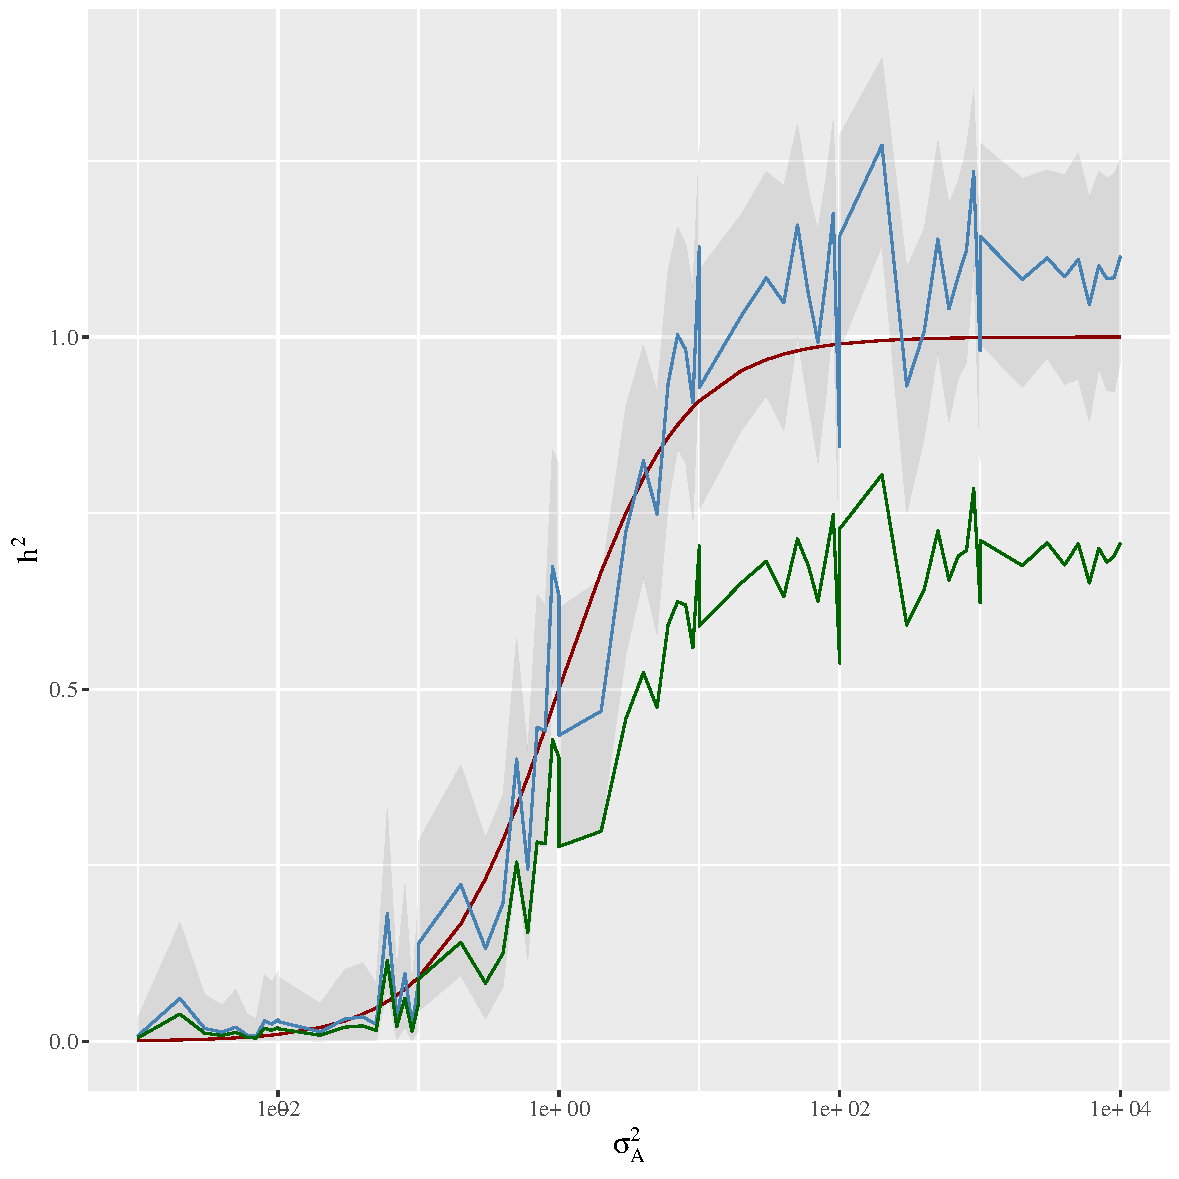
\includegraphics[width=\textwidth]{figures/simulation_deviance_round.pdf}
    \label{fig:simulation_h2_dev:round}
  \end{subfigure}%
  \begin{subfigure}[b]{0.49\textwidth}
    \caption{Binomial dichotomization}
    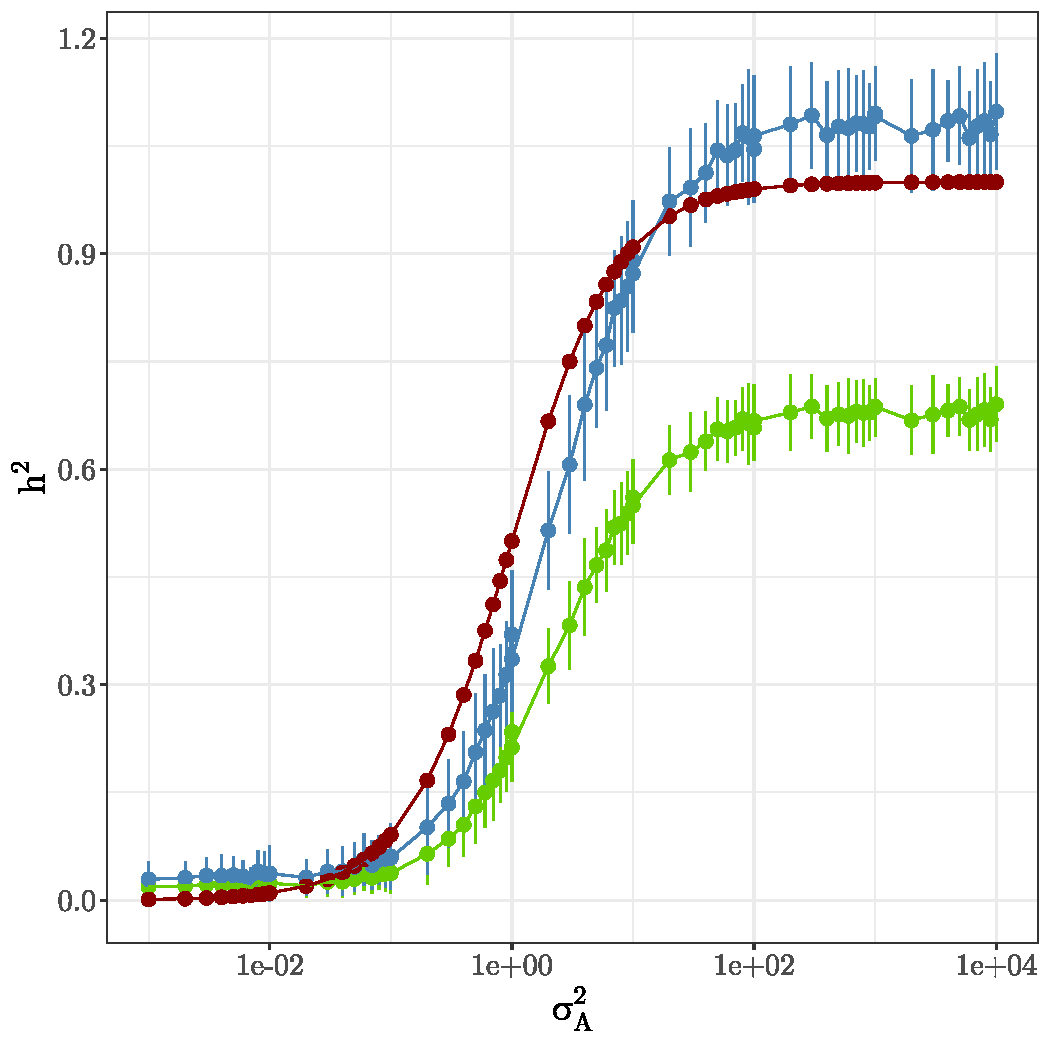
\includegraphics[width=\textwidth]{figures/simulation_deviance_binom.pdf}
    \label{fig:simulation_h2_dev:binom}
  \end{subfigure}
  \begin{subfigure}[b]{0.49\textwidth}
      \caption{Threshold dichotomization for smaller $\sigma^2_A$}
      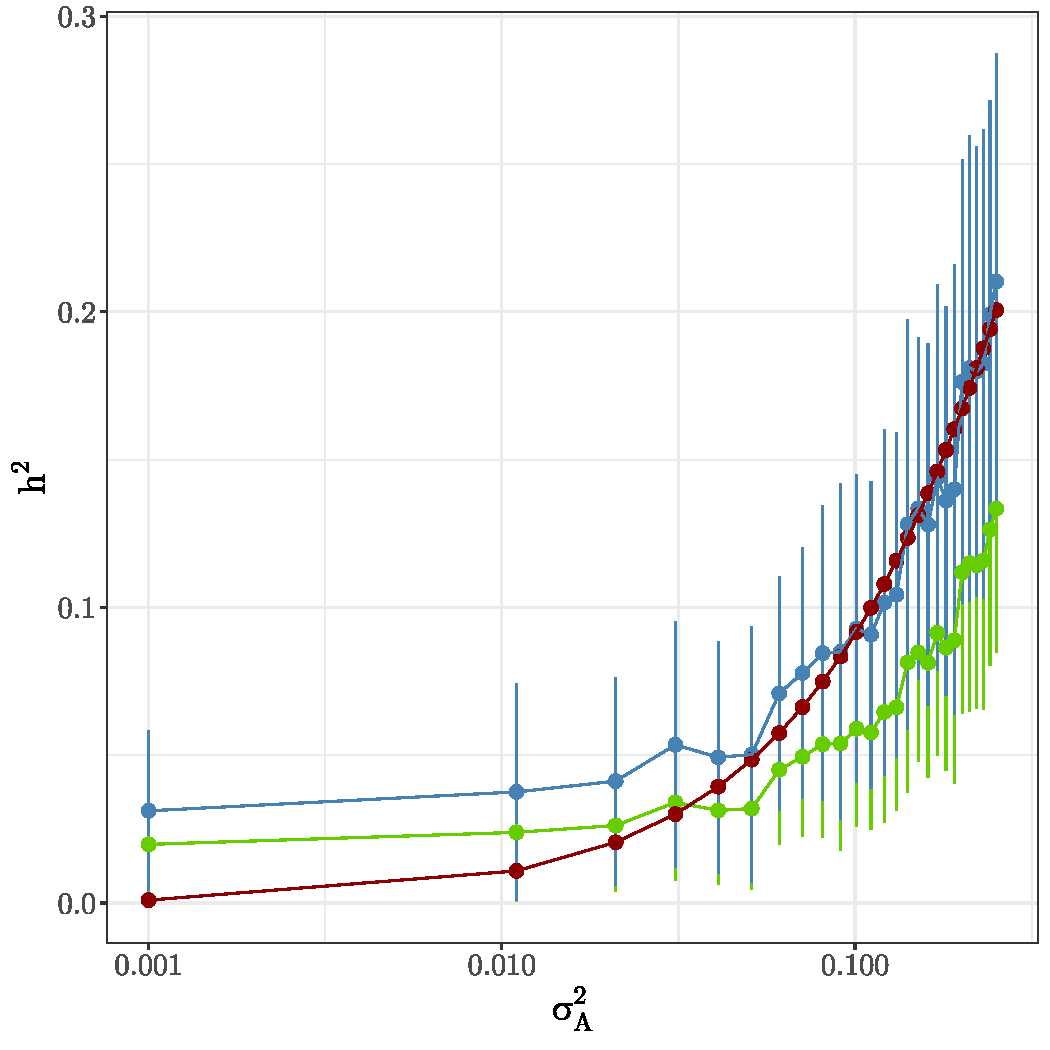
\includegraphics[width=\textwidth]{figures/simulation_deviance_small.pdf}
      \label{fig:simulation_h2_dev:small}
  \end{subfigure}
  \begin{subfigure}[b]{0.49\textwidth}
      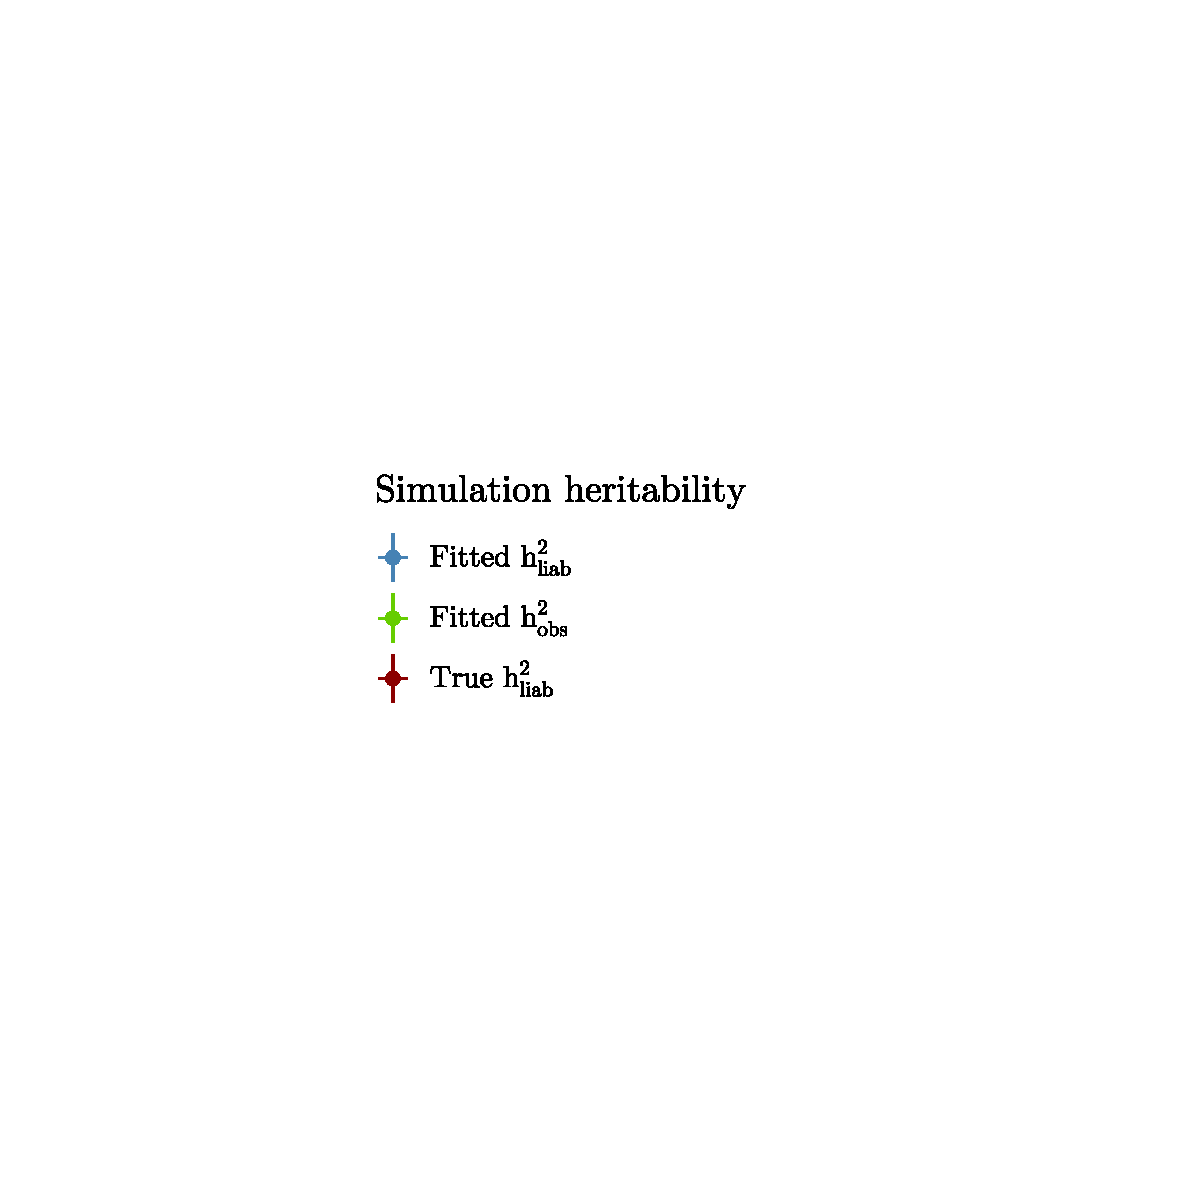
\includegraphics[width=\textwidth, trim={0.7\textwidth} {0.7\textwidth} {0.7\textwidth} {0.7\textwidth},clip]{figures/simulation_deviance_legend.pdf}
  \end{subfigure}
  \caption[Estimated heritability compared to the true value in simulation]{Values of heritabilities for the true, underlying continuous scale in the simulation study (red line), alongside the estimated heritability using a Gaussian model. The green line shows the heritability on the observation scale ($h^2_\text{obs}$) estimated with a Gaussian model using the dichotomized data, whereas the blue line is scaled by the threshold model formula to obtain heritability on the liability scale ($h^2_\text{liab}$). The point shows the mean of 50 runs, with each corresponding line resembling its standard deviation.}
  \label{fig:simulation_h2_dev}
\end{figure}

\subsection{Heritability on different scales}

This section aims to provide an overview of the heritability estimates for its various scales using the simulated data. Initially, we compare the Gaussian and probit models on the liability scale and similarly on the observation scale. Furthermore, we specifically consider the observation-scale heritability of the binomial model ($h^2_\Psi$), where we investigate how changing fixed effects averaging settings may affect $h^2_\Psi$.

The posterior heritability density for the liability and observation scale shows similarities between the Gaussian and probit models for heritability (\autoref{fig:posterior simulation heritability}). The notation and expressions for $h^2_\text{obs}$, $h^2_\text{liab}$, $h^2_\Phi$ and $h^2_\Psi$ are given in \autoref{tab:h2 notation}.
%$h^2_\text{obs}$ is provided from the Gaussian model directly, where $h^2_\text{liab}$ is obtained by multiplying $h^2_\text{obs}$ with the coefficient $p(1-p)/t^2$ \eqref{eq:heritability for threshold model}. Furthermore, $h^2_\Phi$ is the proportion $\hat\sigma^2_A/(\hat\sigma^2_A+\hat\sigma^2_E+1)$ where the estimators are on the latent scale \eqref{eq:link variance h2 phi}, and $h^2_\Psi$ is the back-transformed heritability from the probit model.
Finally, some statistics (the mean, estimated mode, and standard deviation) of the same posteriors are summarized in \autoref{tab:heritability simulation}. Complementary to these results, we report the deviance information criteria for the two models (\autoref{tab:simulation DICs}). In addition to the figures presented here, we refer to \autoref{fig:application gaussian vs binomial} and \autoref{fig:simulatino gaussian vs binomial} in the appendix, providing a grid of density comparisons for the different heritability scales, for the application and simulation data, respectively.

\begin{table}[ht]\centering
% TABLE FROM R: Tue Jun 13 13:48:15 2023 
 \begin{tabular}{lccc}
 \hline
 Model & Mean & Mode & Standard deviation  \\ 
 \hline 

 Gaussian $h^2_\text{obs}$ & 0.131 & 0.117 & 0.049 \\ 
 Probit $h^2_{\Psi}$ & 0.149 & 0.102 & 0.079 \\ 
  & & & \\ 
 Gaussian $h^2_\text{liab}$ & 0.209 & 0.187 & 0.079 \\ 
 Probit $h^2_{\Phi}$ & 0.228 & 0.19 & 0.091 \\ 
 \bottomrule
\end{tabular}


\caption[Heritability means for all scales in simulation]{Heritability estimates for Gaussian and probit models, in the simulation data with $\sigma^2_A=0.5$, showing the mean, mode, and standard deviation. The first two and the last two rows provide heritability comparable to each other. We refer to \autoref{tab:h2 notation} for a reference on how the different scales are computed.}
\label{tab:heritability simulation}
\end{table}

\begin{figure}
    \centering
    \begin{subfigure}{0.49\textwidth}
        \centering
        \caption{Liability scale}
        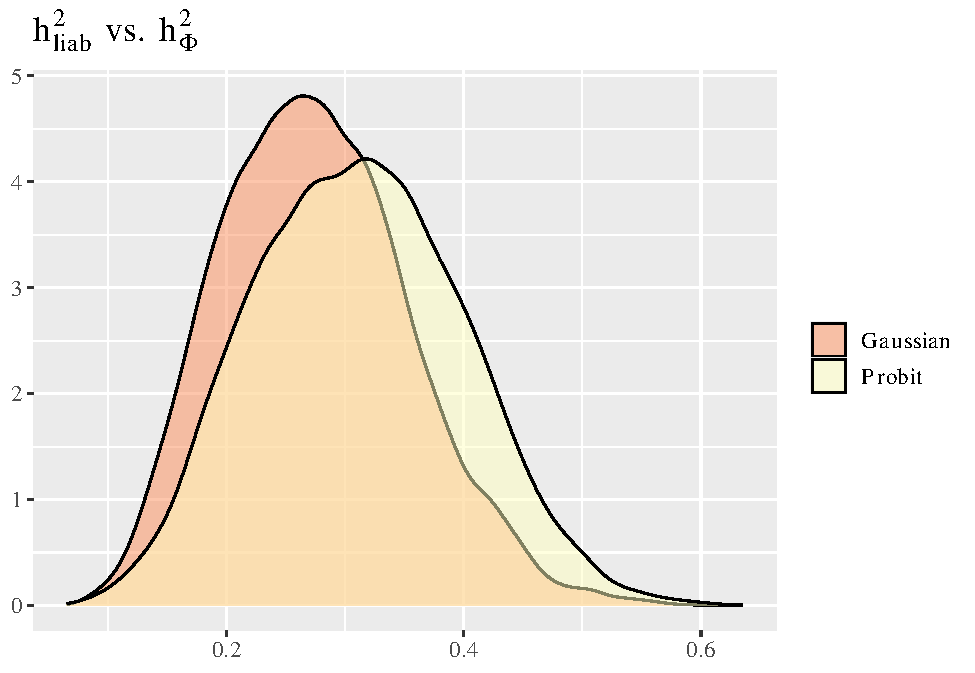
\includegraphics{figures/heritability_simulation_liabscale.pdf}
        \label{fig:posterior simulation heritability:liability}
    \end{subfigure}
    \begin{subfigure}{0.49\textwidth}
        \centering
        \caption{Observation scale}
        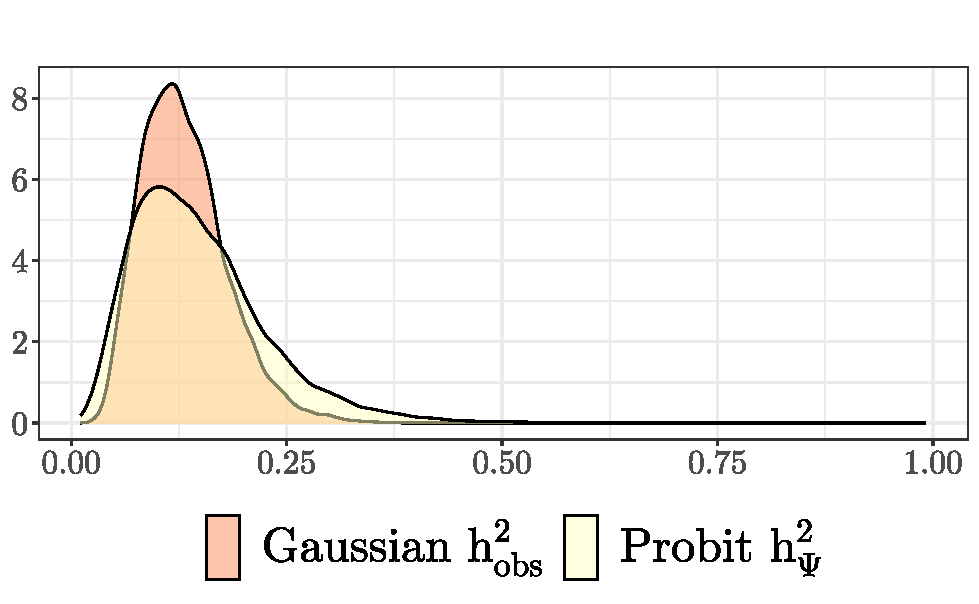
\includegraphics{figures/heritability_simulation_obsscale.pdf}
        \label{fig:posterior simulation heritability:observation}
    \end{subfigure}
    \caption[Heritability density for simulation data]{Posterior liability- and observation-scale densities of heritability for the simulation data.}
    \label{fig:posterior simulation heritability}
\end{figure}

\begin{table}
    \centering
    \begin{tabular}{@{}ll@{}}
    \toprule
        Model           & DIC (Simulation data) \\ \midrule
        Binomial probit & 1180.620 \\
        Gaussian        & 1215.321\\
        \bottomrule
    \end{tabular}
    \caption[DIC for simulation data]{Deviance information criteria (DIC) for the two model fits, for the simulation data, with $\sigma^2_A=0.5$ fixed.}
    \label{tab:simulation DICs}
\end{table}

\subsubsection{Observation scale from probit model}
In the framework from \textcite{de2016general}, there are several parameter settings for computing observation scale heritability $h^2_\Psi$ from binary data, whose difference is described in the methods chapter (\autoref{sec:method:qgglmm settings}). As such, we first investigate to what extent the heritability densities differ from each other. The resulting posteriors for $h^2_\Psi$ are provided in \autoref{fig:qgglmm simulation} for the simulation data, showing little difference for a small $\sigma^2_A=0.1$, although larger deviations for a larger $\sigma^2_A$. In addition to these posteriors, we show the runtime for computing $10,000$ samples in \autoref{tab:h2psi runtime}.

\begin{table}
% Called function at: Wed Apr 26 14:28:32 2023 
% Entering `new.h2.transf` (Bayesian sampling)
% DEBUG: Entering sampling for loop
% DEBUG: Entering transposing loop
% Done after 3.327576 minutes. Entering same function without the Bayesian stuff.
% Done after 0.1665074 minutes. Now without averaging:Done after 0.06656845 minutes.
% Saving to disk...
% [1] 0
    \centering
    \begin{tabular}{@{}lr@{}}
    \toprule
    Estimate & Runtime \\ \midrule
    $h^2_\Psi$ Bayesian & $26$ sec \\
    $h^2_\Psi$ Frequentist & $11$ sec \\
    $h^2_\Psi$ No averaging & $4$ sec \\
    \bottomrule
    \end{tabular}
    \caption[Runtime of computing $h^2_\Psi$]{Runtime of computing $10,000$ samples of $h^2_\Psi$ in seconds for the three methods provided by the \texttt{QGglmm} package, in simulation data with $900$ observations.}
    \label{tab:h2psi runtime}
\end{table}


% <<<<< QGglmm comparisons
\begin{figure}
    \centering
    \begin{subfigure}[b]{0.49\textwidth}
        \caption{$\sigma^2_A=0.1$}
        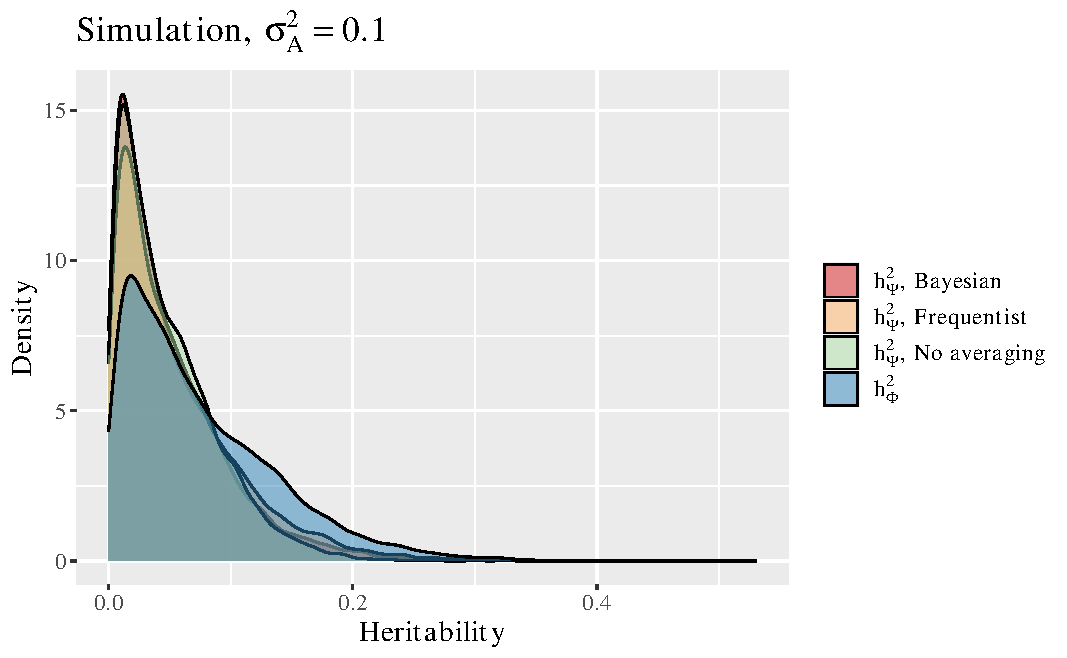
\includegraphics[width=\textwidth]{figures/qgglmm-comparison-simulationva0.1.pdf}     
    \end{subfigure}
    \begin{subfigure}[b]{0.49\textwidth}
        \caption{$\sigma^2_A=1$}
        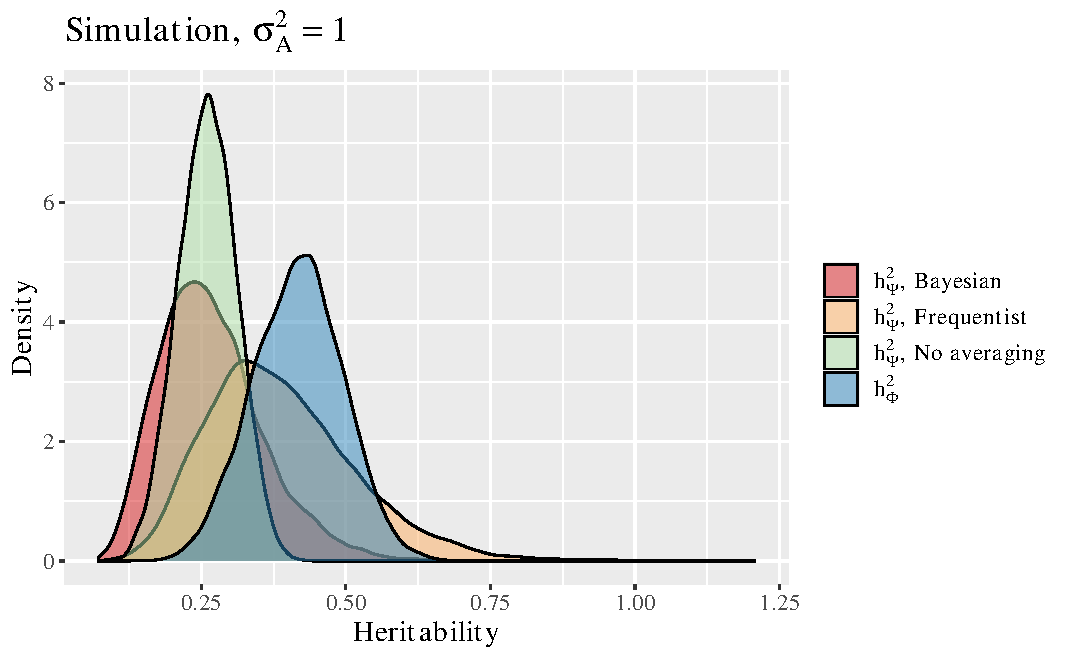
\includegraphics[width=\textwidth]{figures/qgglmm-comparison-simulationva1.pdf}\label{fig:qgglmm simulation:bigvA}
    \end{subfigure}
    \begin{subfigure}[b]{0.25\textwidth}
    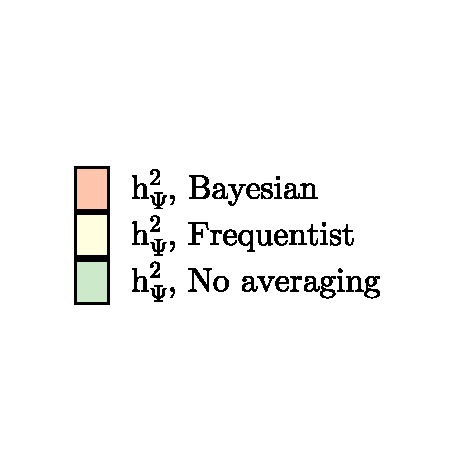
\includegraphics[width=\textwidth, trim={0.3\textwidth} {0.3\textwidth} {0.3\textwidth} {0.3\textwidth},clip]{figures/qgglmm-comparison-simulation-legend.pdf}
    \end{subfigure}
    \caption[$h^2_\Psi$ on simulations, with varying parameter settings]{Estimated posterior heritability for the different back-transformations techniques, for a binomial probit model to simulations with small variance ($\sigma^2_A=0.1$) and a simulation with larger variance ($\sigma^2_A=1$), respectively.}
    \label{fig:qgglmm simulation}
\end{figure}


% >>>>> QGglmm comparisons

%In the application case, all three discussed methods for computing $h^2_\Psi$ are very similar.
% Now, we want to see what the Gaussian model looks like compared to the other methods. The notation here is described in \autoref{tab:h2 notation}. %% ???
\subsection{Robustness tests}
Lastly, we present some results exploring the robustness of the models, namely by introducing fixed effects and overdispersion. \autoref{fig:fixed effects sim deviance gaussian model} illustrates how the heritability of the Gaussian model, once transformed to its liability scale, is relative to the theoretical value for varying values of $\sigma^2_A$. In this context, the theoretical value includes fixed effects variance in the denominator, \autocite{nakagawa2013general}
\begin{equation}
    h^2_\text{liab} = \frac{\sigma^2_A}{\sigma^2_A + \sigma^2_E + \beta_\text{sex}^2\sigma^2_{\text{sex}}} \ .
\end{equation}

The plot is similar to \autoref{fig:simulation_h2_dev}, although the subplots differ in the magnitude of the fixed effect term rather than different dichotomization methods. We can also see a significant deviation between the estimated and true $h^2_\text{liab}$ for the case of fixed effects. Additionally, we provide the posterior density of heritability when including fixed effects to assess differences quantitatively (\autoref{fig:fixedeffects probit vs gaussian}). The plot shows the posterior heritabilities for a Gaussian and a probit model fitted on simulation data where $\beta_{\text{sex}}=10$, $\sigma^2_E=1$, and varying $\sigma^2_A$ and $\hat p$. It seems like the estimate from the Gaussian and probit models differ more in the presence of fixed effects.
The second robustness factor examined is overdispersion. The heritability of the resulting models for varying $\sigma^2_E$ are shown in \autoref{fig:overdisperion plots}, where generally all models seem to produce similar posterior heritability estimates.

\begin{figure}
    \centering
    \begin{subfigure}{0.49\textwidth}
    \caption{}
        % \caption{$\beta_\text{sex}=10$, unbalanced $p = 0.1$ for each simulation.}
        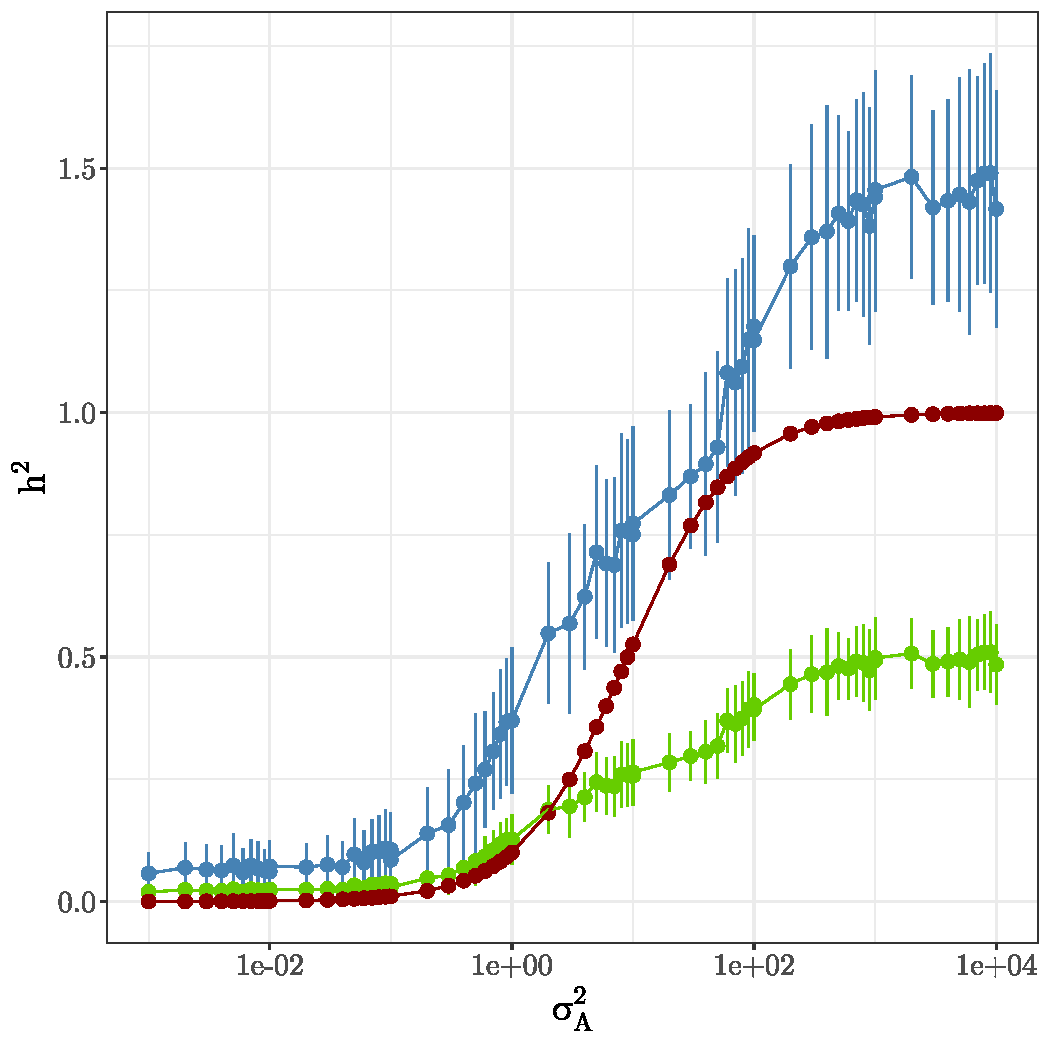
\includegraphics[width=\linewidth]{figures/simulation_deviance_fixedeffects_beta10_unbalanced.pdf}
    \end{subfigure}
    \begin{subfigure}{0.49\textwidth}
    \caption{}
        % \caption{$\beta_\text{sex}=10$, balanced $p\in [0.48, 0.52]$ with 95\% confidence.}
        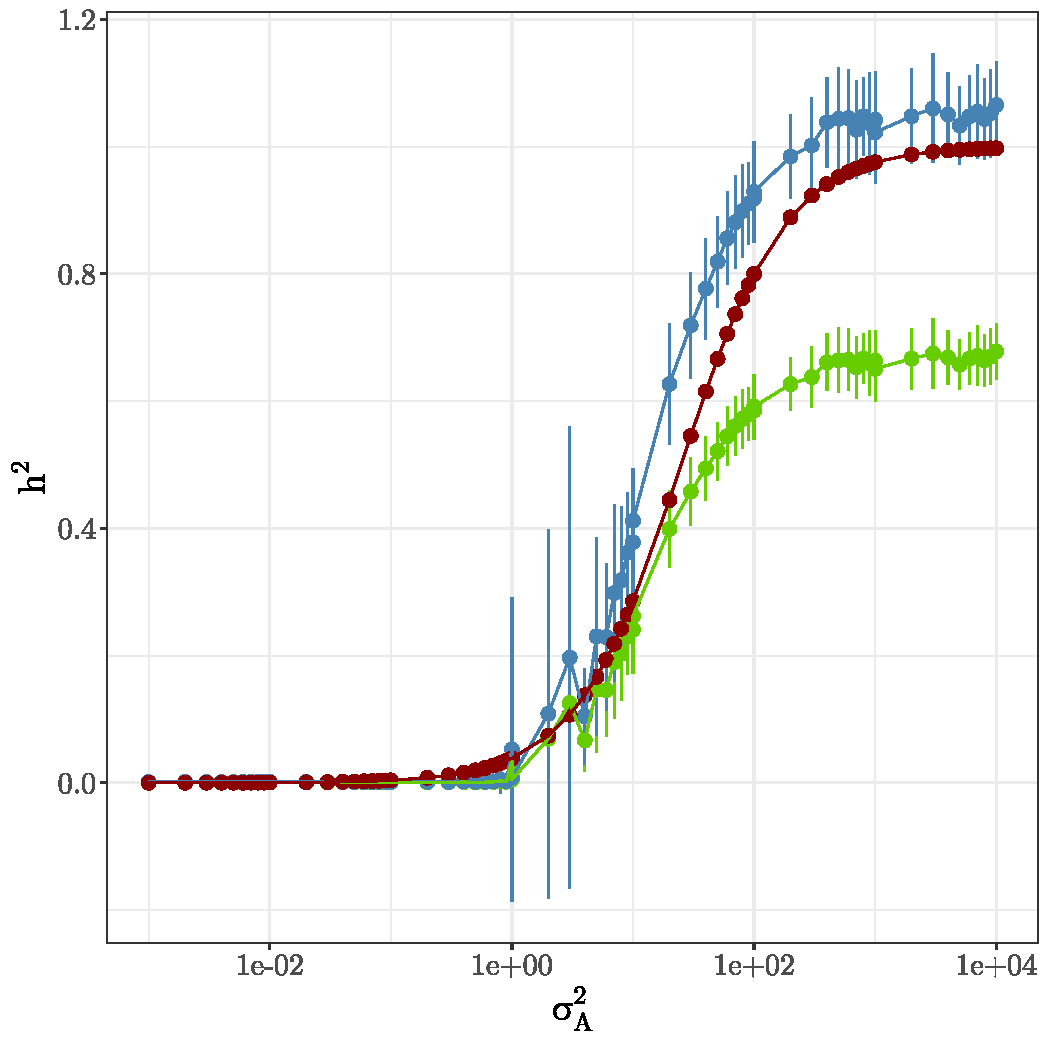
\includegraphics[width=\linewidth]{figures/simulation_deviance_fixedeffects_beta10.pdf}
    \end{subfigure}
        \begin{subfigure}{0.49\textwidth}
        \caption{}
        % \caption{$\beta_\text{sex}=100$, balanced $p \in [0.49, 0.51]$ with 95\% confidence.}
        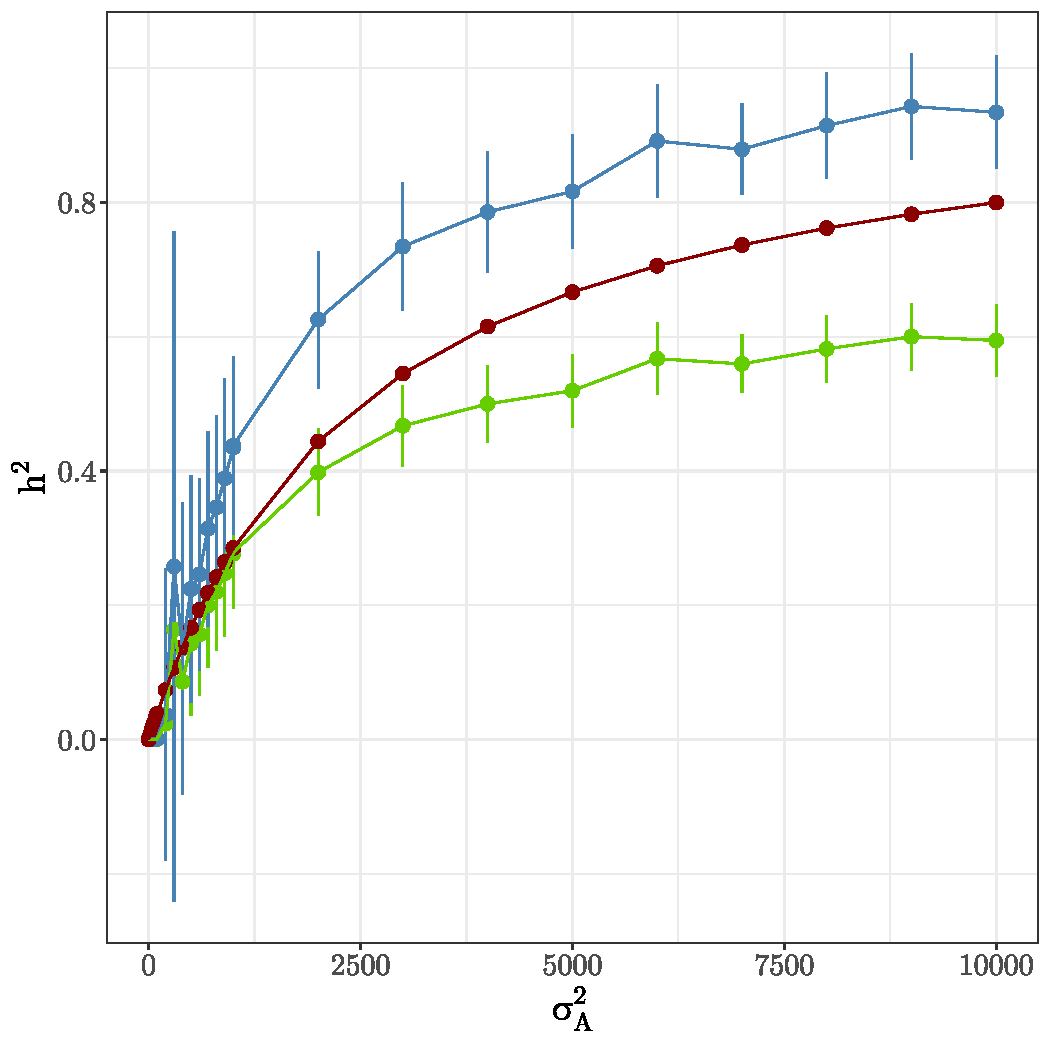
\includegraphics[width=\linewidth]{figures/simulation_deviance_fixedeffects_beta100.pdf}
    \end{subfigure}
    \begin{subfigure}{0.49\textwidth}
        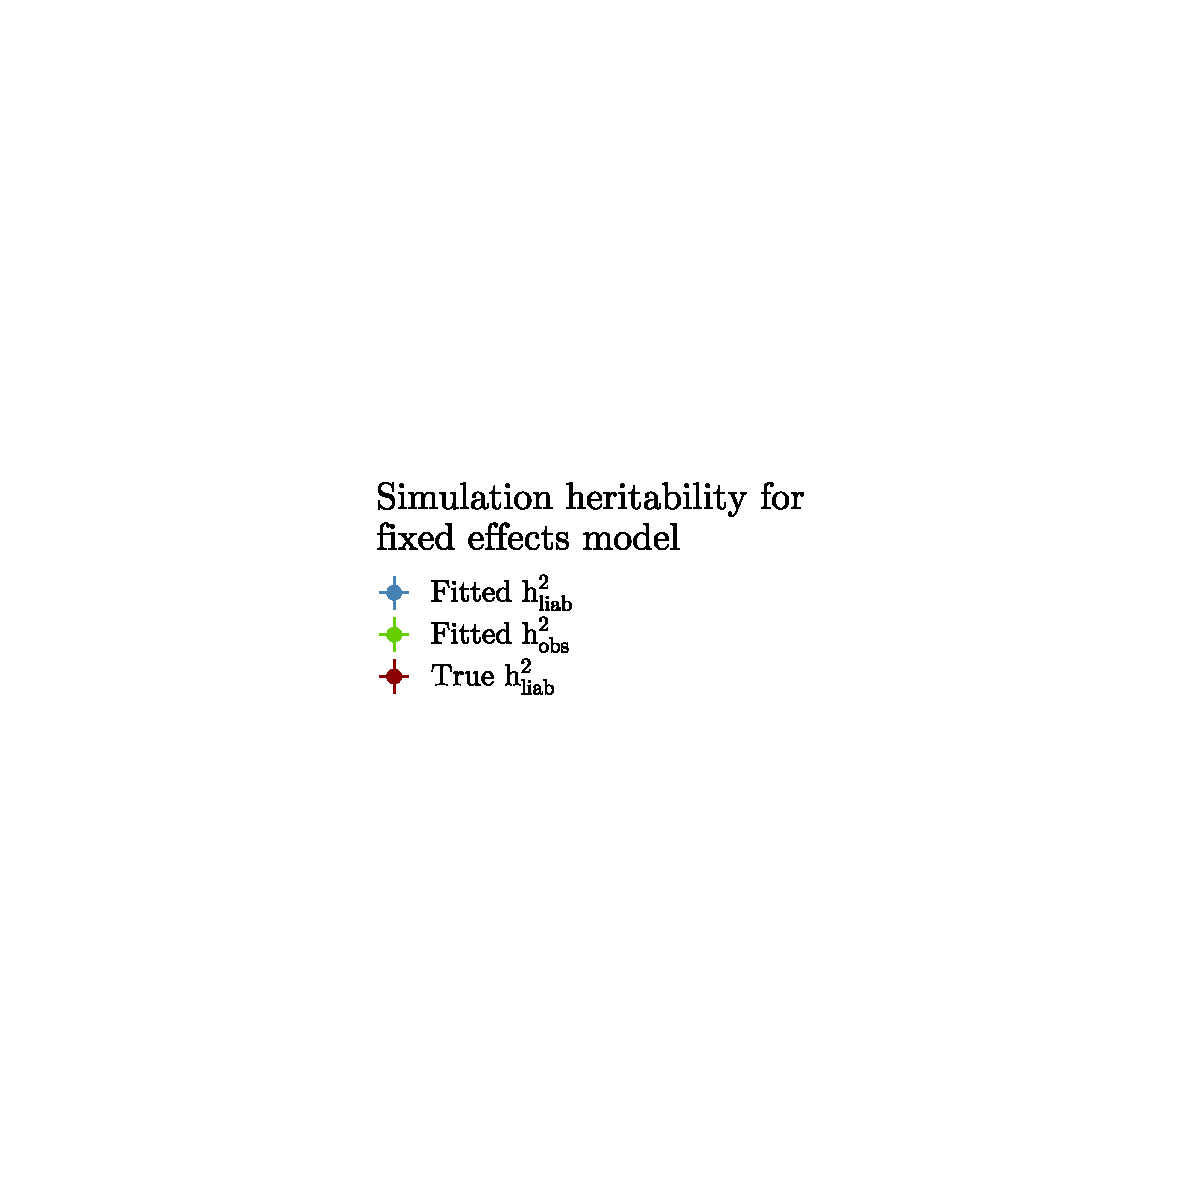
\includegraphics[width=\linewidth, trim={0.7\textwidth} {0.7\textwidth} {0.7\textwidth} {0.7\textwidth},clip]{figures/simulation_deviance_fixedeffects_legend.pdf}
    \end{subfigure}
    \caption[Estimated $h^2_\text{liab}$ compared to true value for fixed effects models]{Estimates for heritability with a Gaussian model including fixed effects. The red line shows the true heritability on the liability scale and includes fixed effects variance as part of phenotypic variance. Subfigure \textbf{(a)} shows the results for an unbalanced $\hat p=0.1$ and $\beta_\text{sex}=10$, whereas the phenotypic mean is balanced in the other subfigures. Furthermore, subfigure \textbf{(b)} demonstrate $\beta_\text{sex}=10$ and \textbf{(c)} with $\beta_\text{sex}=100$. The points show the mean over 50 runs with each corresponding line resembling its standard deviation.}
    \label{fig:fixed effects sim deviance gaussian model}
\end{figure}

\begin{figure}
    \centering
    \begin{subfigure}{0.49\textwidth}
    \caption{$\beta=10$, $\sigma^2_A=10$, $\sigma^2_E=1$, $\hat p=0.1$}
    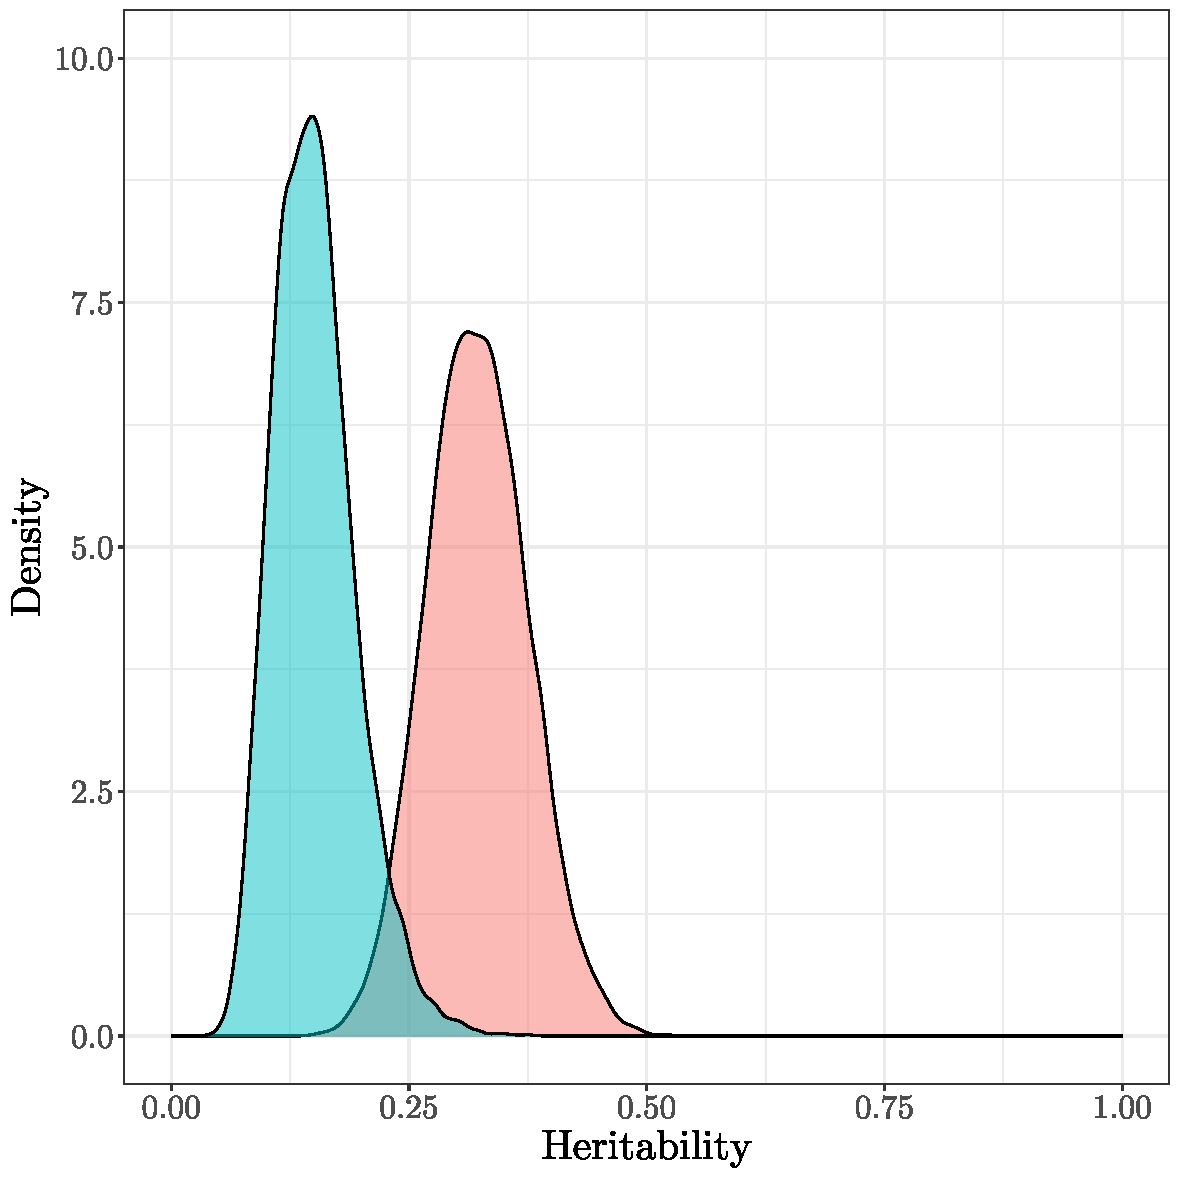
\includegraphics[width=\textwidth]{figures/fixedeffects_gaussian_probit_sA10_p_1.pdf}
    \label{fig:fixedeffects probit vs gaussian:lVAlP}
    \end{subfigure}
    \begin{subfigure}{0.49\textwidth}
    \caption{$\beta=10$, $\sigma^2_A=10$, $\sigma^2_E=1$, $\hat p=0.5$}
    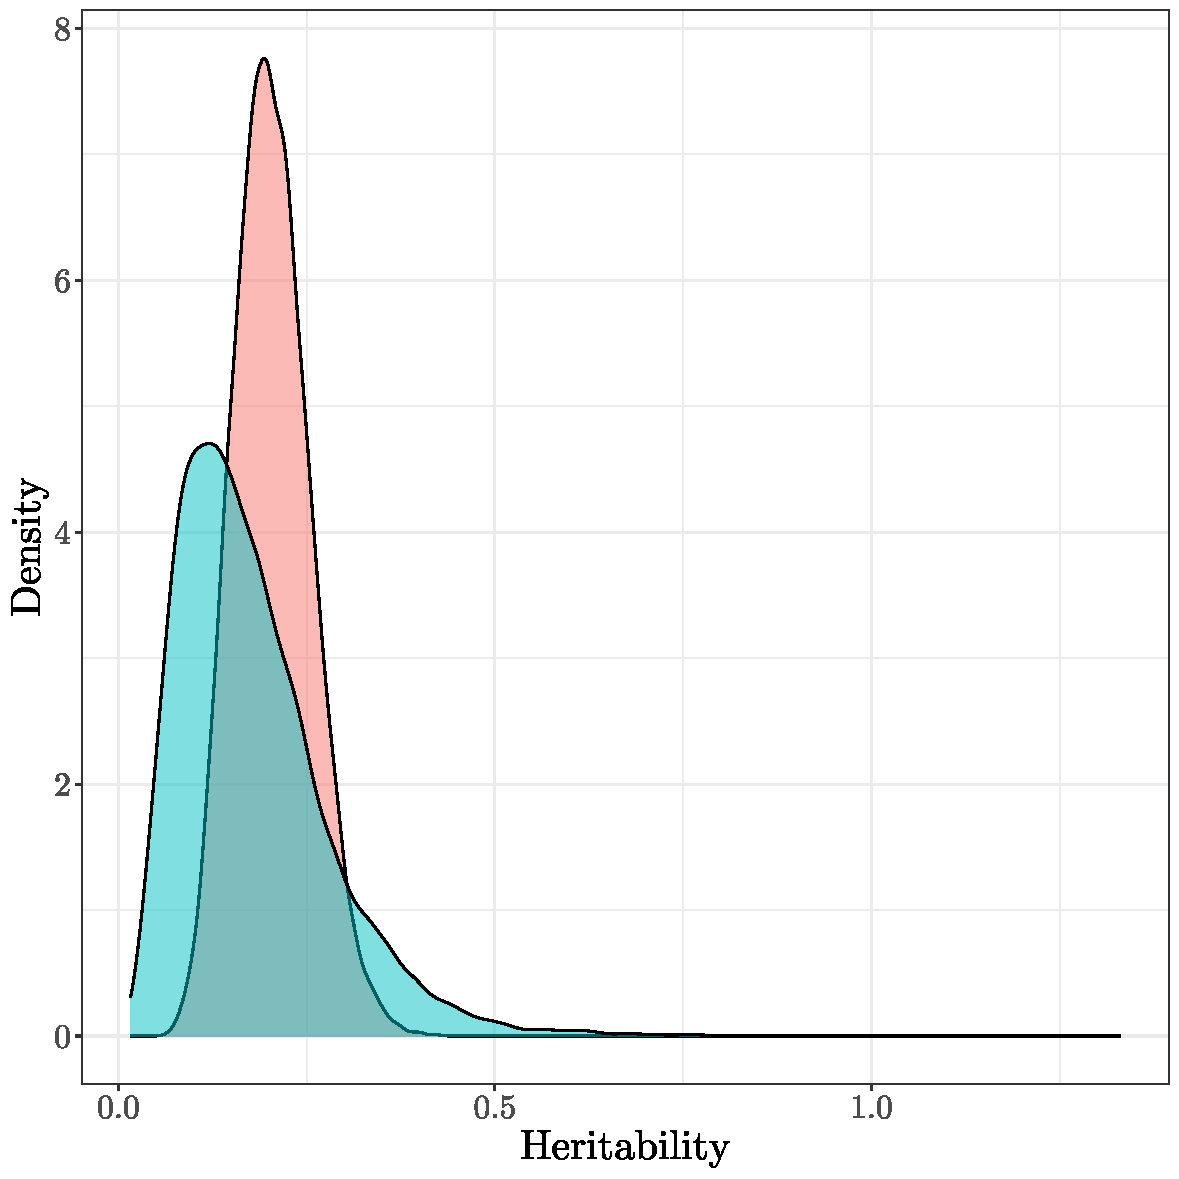
\includegraphics[width=\textwidth]{figures/fixedeffects_gaussian_probit_sA10_p_5.pdf}
    \label{fig:fixedeffects probit vs gaussian:lVAhP}
    \end{subfigure}
    \begin{subfigure}{0.49\textwidth}
    \caption{$\beta=10$, $\sigma^2_A=500$, $\sigma^2_E=1$, $\hat p=0.1$}
    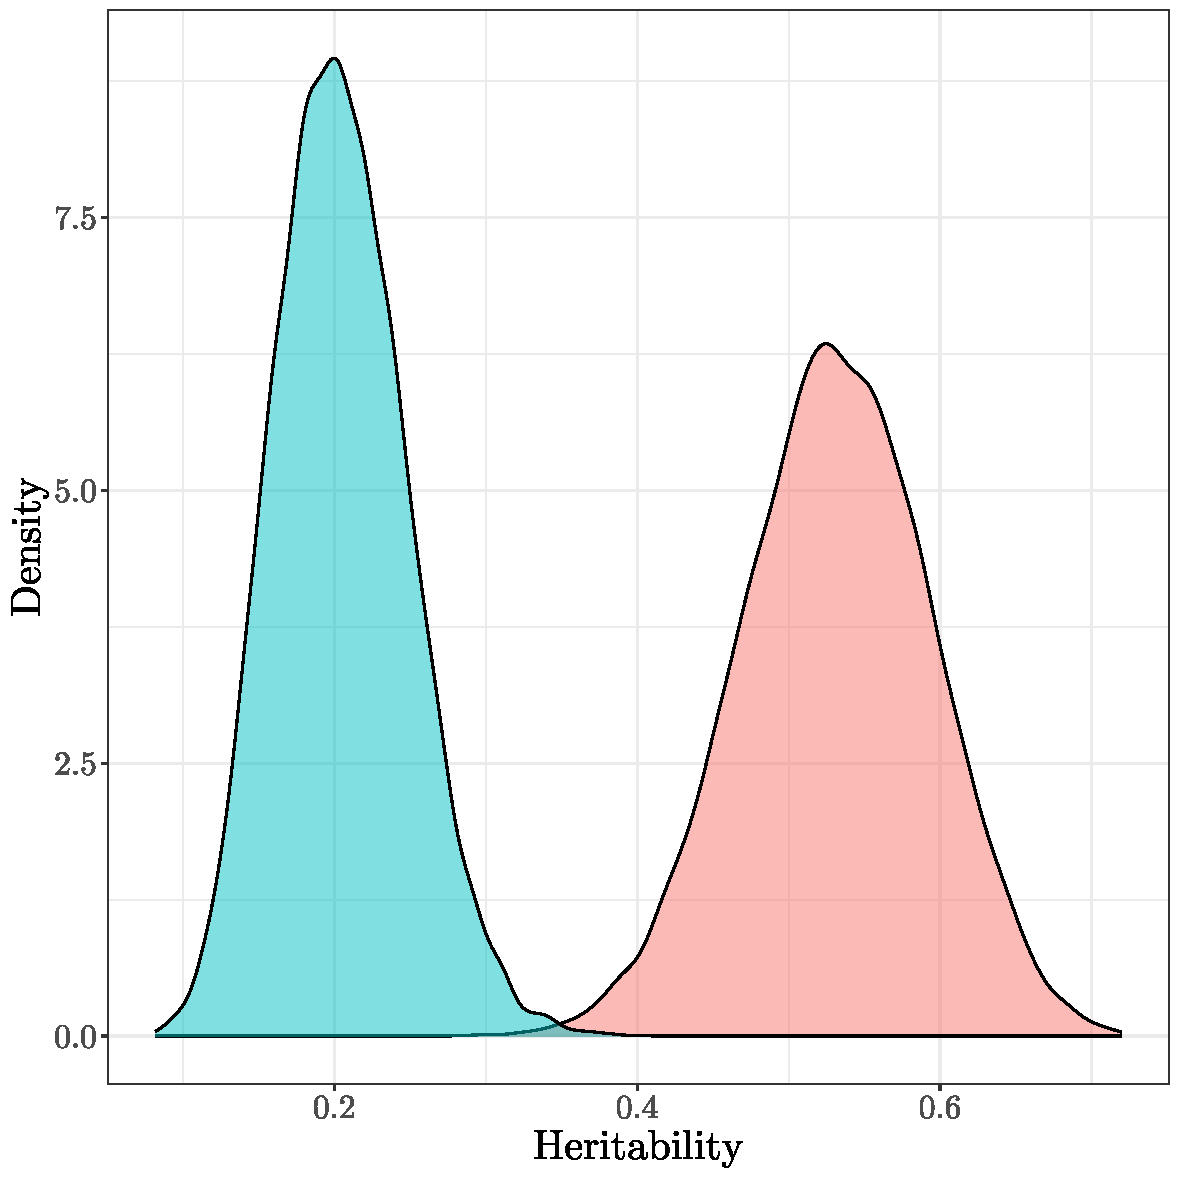
\includegraphics[width=\textwidth]{figures/fixedeffects_gaussian_probit_sA500_p_1.pdf}
    \label{fig:fixedeffects probit vs gaussian:hVAlP}
    \end{subfigure}
    \begin{subfigure}{0.49\textwidth}
    \caption{$\beta=10$, $\sigma^2_A=500$, $\sigma^2_E=1$, $\hat p=0.5$}
    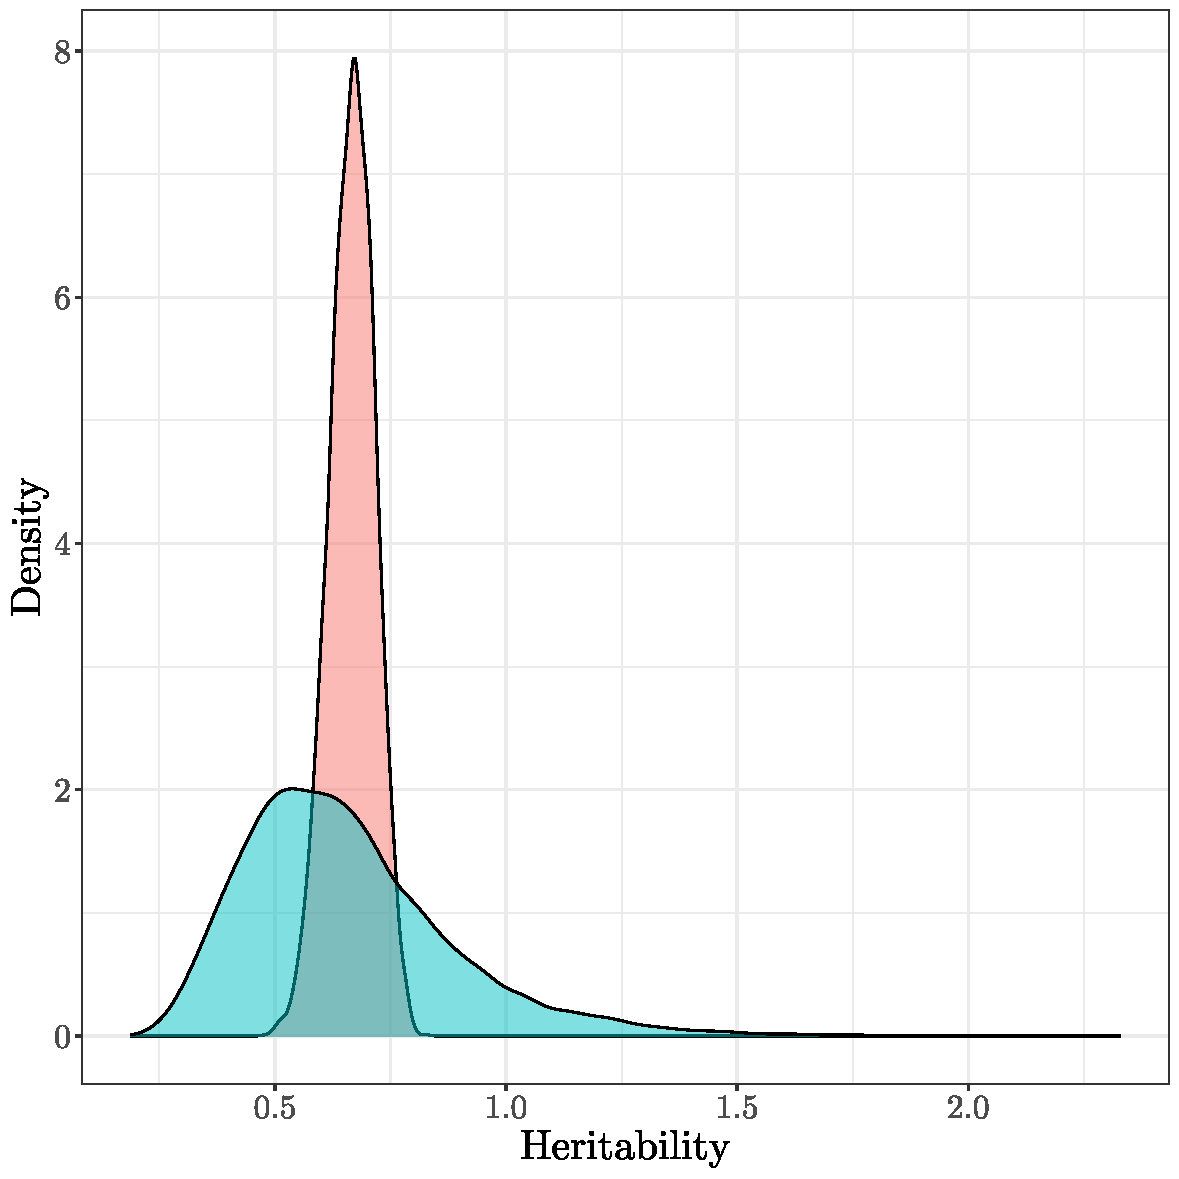
\includegraphics[width=\textwidth]{figures/fixedeffects_gaussian_probit_sA500_p_5.pdf}
    \label{fig:fixedeffects probit vs gaussian:hVAhP}
    \end{subfigure}
    \begin{subfigure}{0.6\textwidth}
    
\includegraphics[width=\textwidth]{figures/fixedeffects_gaussian_probit_legend.pdf}
    \end{subfigure}
    \caption[$h^2$ for fixed effects simulation models]{Posterior heritability for simulations with fixed effects on observation-scale. The first column shows the results with an unbalanced trait, $p=0.1$, and the other column for a balanced trait $p=0.5$. Furthermore, the first row show densities where $\sigma^2_A=10$, and the second row when $\sigma^2_A=500$.}
    \label{fig:fixedeffects probit vs gaussian}
\end{figure}
% \begin{figure}
%     \centering
%     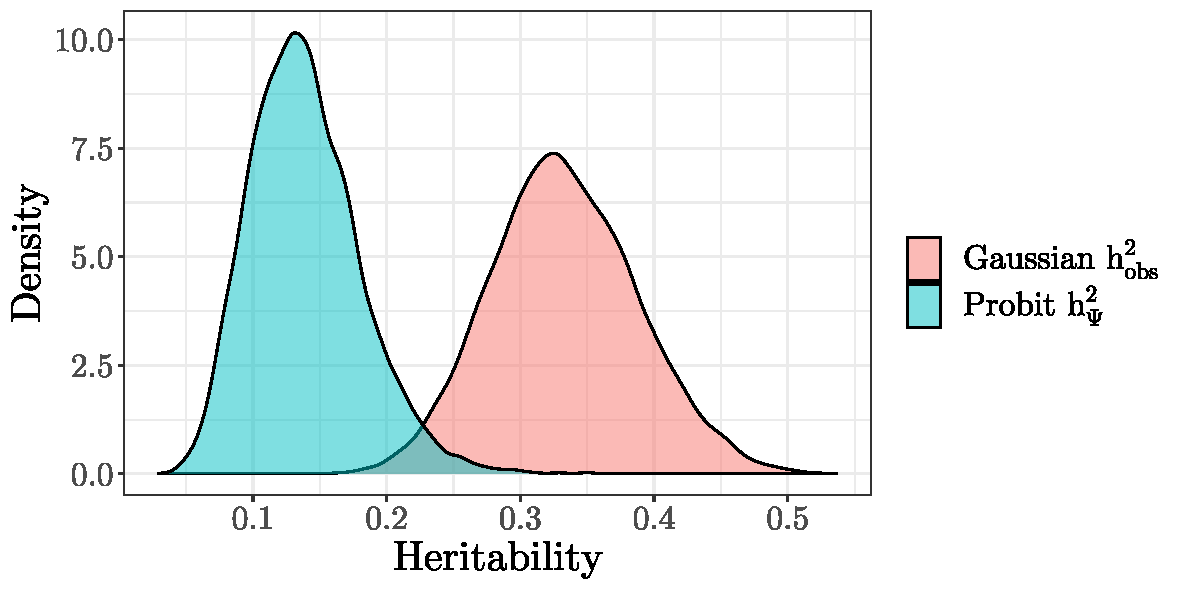
\includegraphics{figures/density-fixed/fixedeffects_gaussian_probit_sA10_p_1_wide.pdf}
%     \caption[$h^2$ density on observation scale for fixed effects model]{A comparison between the posterior heritability on observation-scale for a Gaussian (red) and binomial probit model (blue), the latter of which is back-transformed by \autoref{alg:qgglmm-probit}. The dashed, dark red line shows the theoretical observation-scale heritability in the simulation model. That is, threshold-scaled $h^2_\text{obs}$ for the corresponding $h^2_\text{liab}=\sigma^2_A/(\sigma^2_A+\sigma^2_E+\Var{\beta_\text{sex}\bf x_{\text{sex}}})$. In this particular case, $\beta=10$, $\sigma^2_A=10$ and $\sigma^2_E=1$. }
%     \label{fig:fixedeffects probit vs gaussian vs true}
% \end{figure}


\begin{figure}[H]
    \centering
    \begin{subfigure}{0.49\textwidth}
        \caption{$\sigma^2_A=0.5$, $\sigma^2_E=2$}
        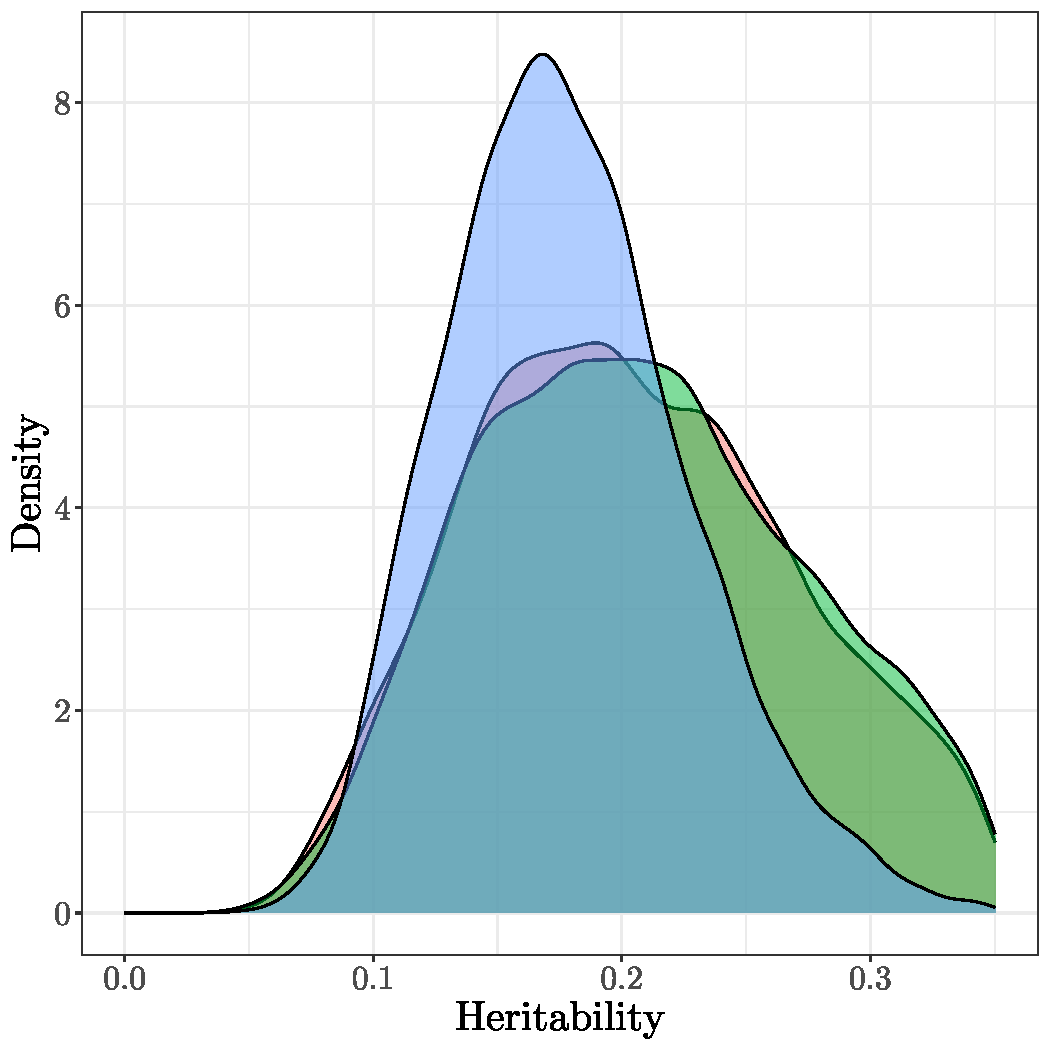
\includegraphics[width=\linewidth]{figures/overdispersion_vE-vA_2-0.5.pdf}
    \end{subfigure}
    \begin{subfigure}{0.49\textwidth}
        \caption{$\sigma^2_A=0.5$, $\sigma^2_E=5$}
        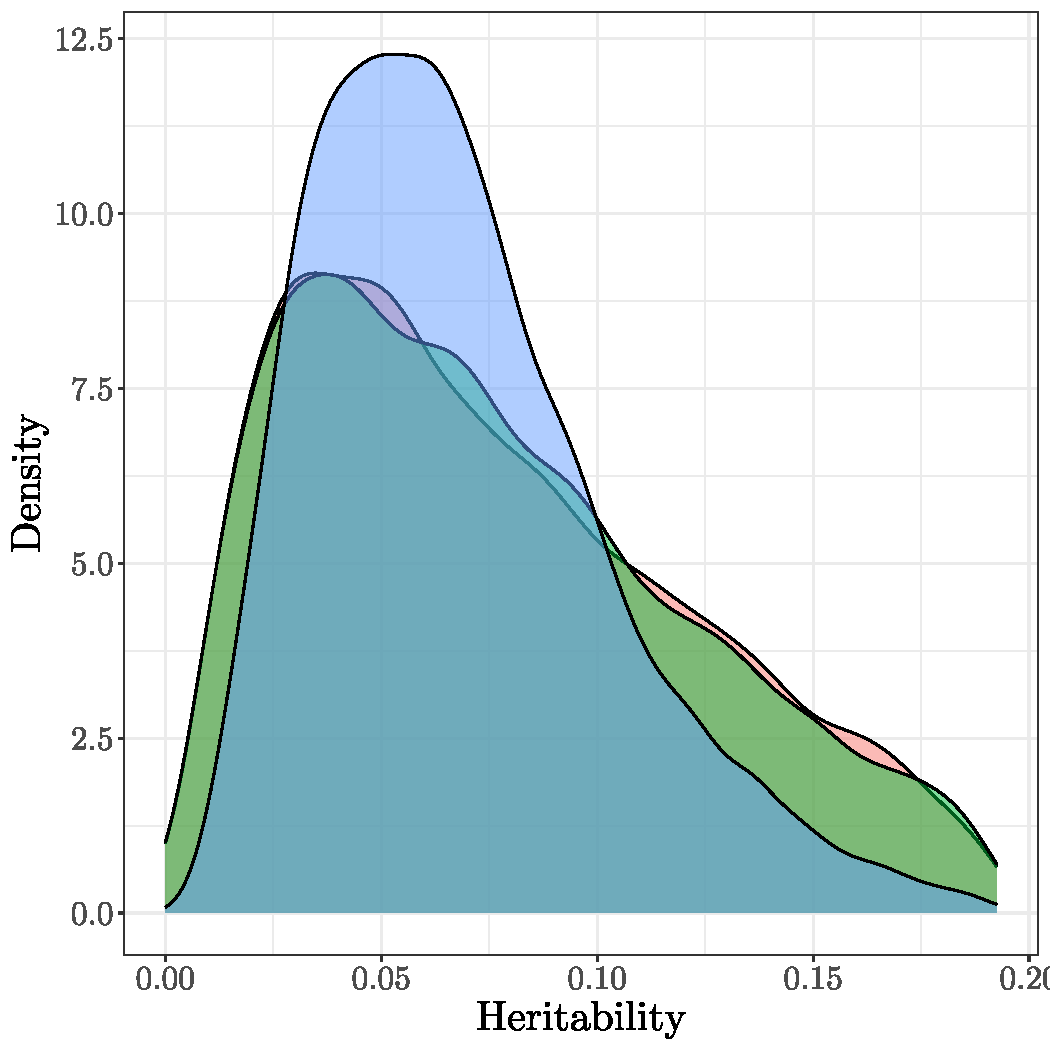
\includegraphics[width=\linewidth]{figures/overdispersion_vE-vA_5-0.5.pdf}
    \end{subfigure}
    \begin{subfigure}{0.49\textwidth}
        \caption{$\sigma^2_A=0.5$, $\sigma^2_E=10$}
        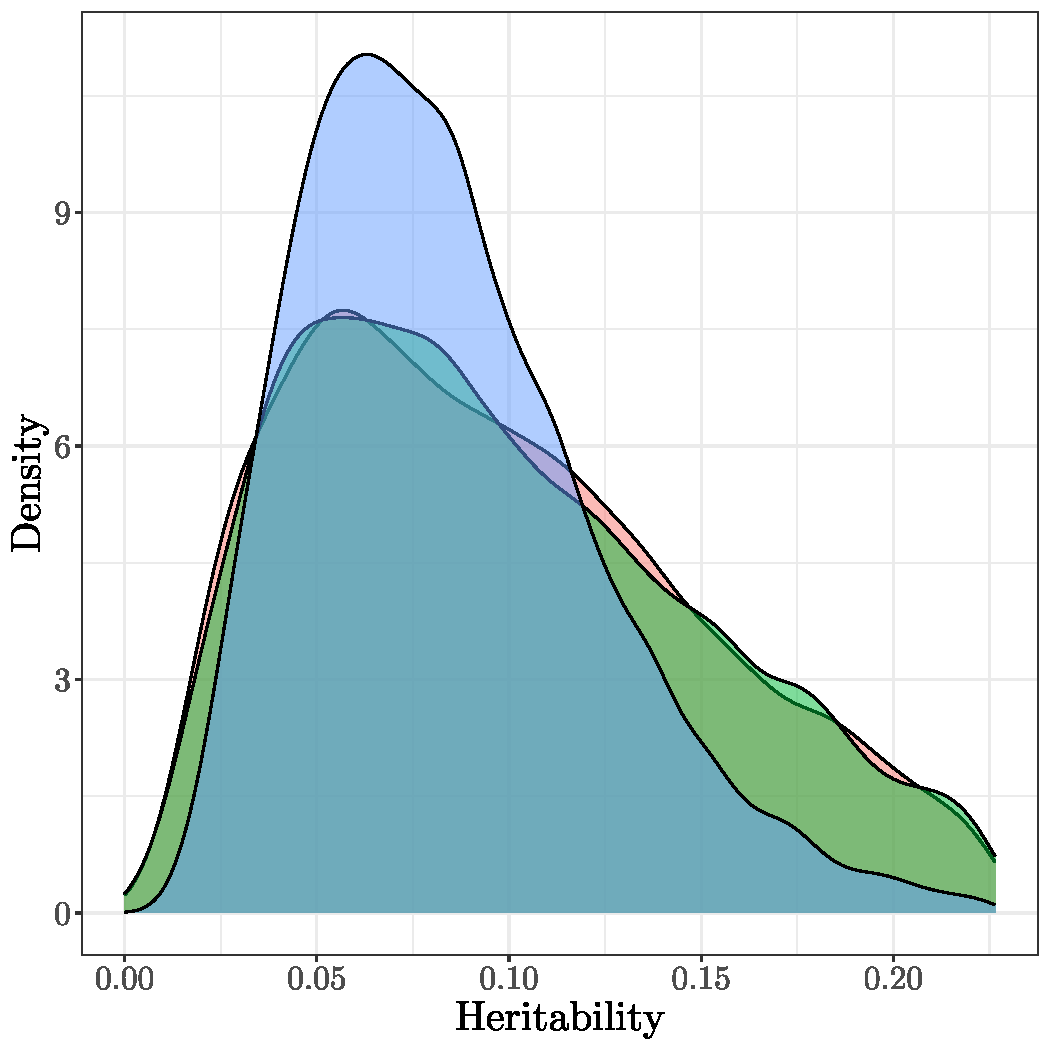
\includegraphics[width=\linewidth]{figures/overdispersion_vE-vA_10-0.5.pdf}
    \end{subfigure}
    \begin{subfigure}{0.49\textwidth}
        \caption{$\sigma^2_A=10$, $\sigma^2_E=10$}
        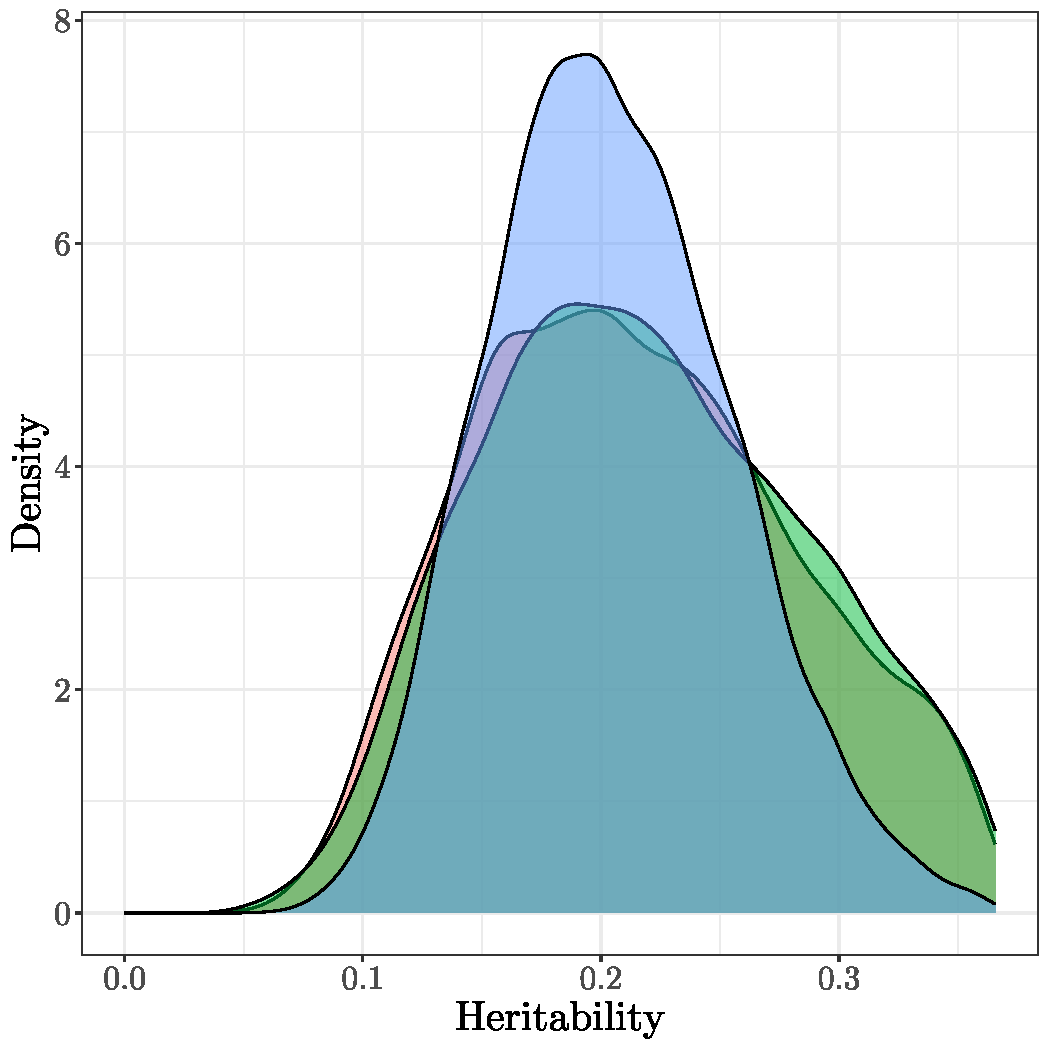
\includegraphics[width=\linewidth]{figures/overdispersion_vE-vA_10-10.pdf}
    \end{subfigure}
    \begin{subfigure}{\textwidth}
        
\includegraphics[width=\textwidth]{figures/overdisperions_legend.pdf}
    \end{subfigure}
    \caption[Posterior with and without overdispersion (simulation data)]{A comparison between two probit models and a Gaussian model fitted with the simulation data. One of the probit models has an additional random iid effect to account for overdispersion, whereas the other does not have the random iid effect. The heritability densities are shown for varying $\sigma^2_A$ and $\sigma^2_E$. %The dashed, dark red line resembles the true observation scale heritability for the simulation.
    }
    \label{fig:overdisperion plots}
\end{figure}


\section{Application study}

\subsection{Heritability on different scales}
Replicating the method in the previous section, we present the heritability estimates for the application data. They are provided in \autoref{fig:posterior application heritability} and \autoref{tab:heritability application}, showing similarities between the heritability of the Gaussian and probit models on the respective scales. Similarly to the simulation case, we employ the different parameter settings in the algorithm for observation-scale heritability from the probit model, yielding \autoref{fig:qgglmm application}.
 
\begin{table}[ht]\centering
% TABLE FROM R: Tue Jun 13 13:48:14 2023 
 \begin{tabular}{lccc}
 \hline
 Model & Mean & Mode & Standard deviation  \\ 
 \hline 

 Gaussian $h^2_\text{obs}$ & 0.034 & 0.025 & 0.018 \\ 
 Probit $h^2_{\Psi}$ & 0.03 & 0.02 & 0.016 \\ 
  & & & \\ 
 Gaussian $h^2_\text{liab}$ & 0.062 & 0.046 & 0.032 \\ 
 Probit $h^2_{\Phi}$ & 0.055 & 0.042 & 0.027 \\ 
 \bottomrule
\end{tabular}

\caption[Heritability means for all scales in application data]{Heritability estimates for the Gaussian and probit models, in the application data, showing the mean, mode, and standard deviation. The first and last two rows provide heritability comparable to one another. We refer to \autoref{tab:h2 notation} for a reference on how the different scales are computed.}
\label{tab:heritability application}
\end{table}

\begin{figure}
    \centering
    \begin{subfigure}{0.49\textwidth}
        \centering
        \caption{Liability scale}
        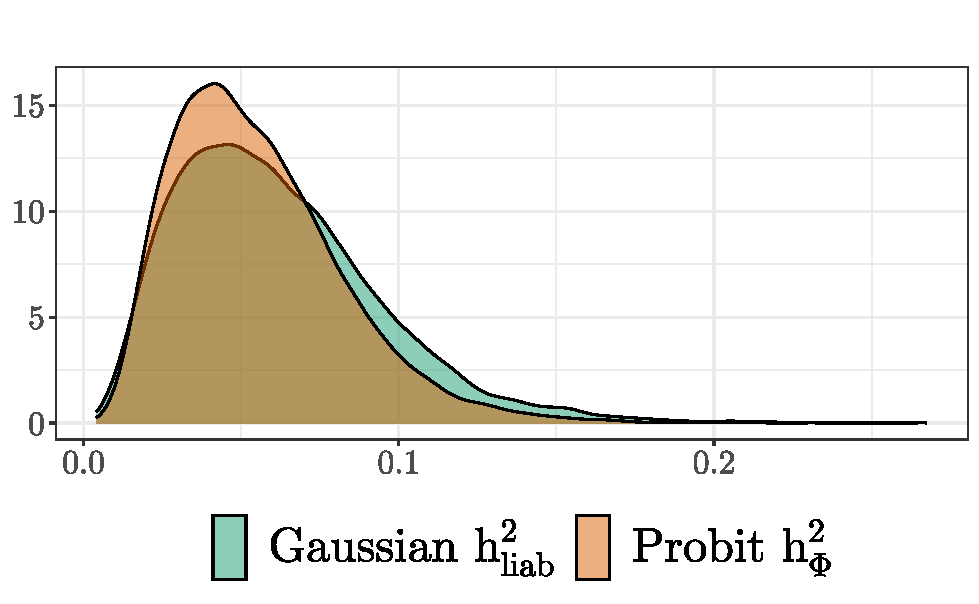
\includegraphics{figures/heritability_application_liabscale.pdf}
        \label{fig:posterior application heritability:liability}
    \end{subfigure}
    \begin{subfigure}{0.49\textwidth}
        \centering
        \caption{Observation scale}
        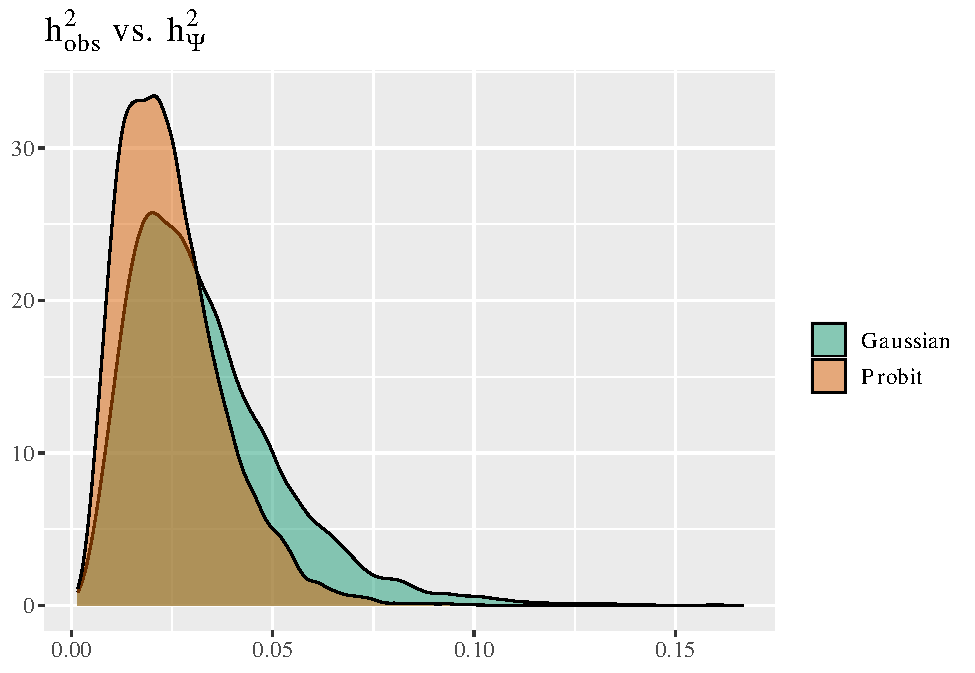
\includegraphics{figures/heritability_application_obsscale.pdf}
        \label{fig:posterior application heritability:observation}
    \end{subfigure}
    \caption[Heritability density for application data]{Posterior liability- and observation-scale densities of heritability for the application data.}
    \label{fig:posterior application heritability}
\end{figure}


\begin{figure}
    \centering
        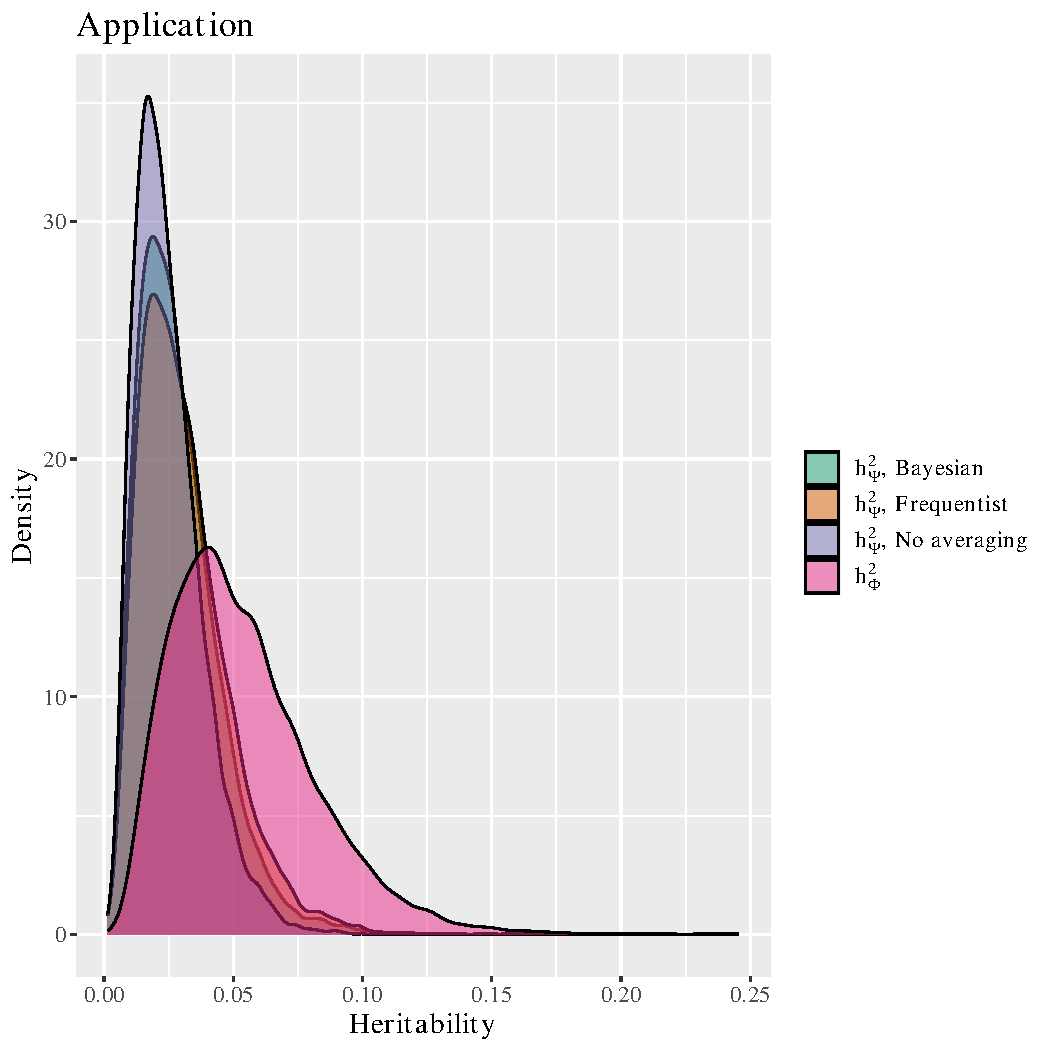
\includegraphics[width=0.8\textwidth]{figures/qgglmm-comparison-application.pdf}       
    \caption[$h^2_\Psi$ on application data, with varying parameter settings]{Estimated posterior heritability for the different back-transformations techniques, for a binomial probit model to the application data.}
    \label{fig:qgglmm application}
\end{figure}
\subsection{Gaussian residual analysis}
In addition to computing the estimated heritability, we would like to explore the residual distribution of the Gaussian model for the application dataset. We fit a Gaussian model using INLA to the application data, in which we also compute the model's PIT values to evaluate the goodness of fit. \autoref{fig:sorted pit values} shows the sorted PIT values in ascending order relative to their quantiles, which would resemble a straight line for a uniform distribution, which is not the case for our data. \autoref{fig:gaussian pit vs fitted} shows the PIT values over the mean of the posterior fitted values, as well as a cubic spline smoothing plot. The PIT values show a clear pattern rather than being uniformly distributed, which is also the case for the plot of the residuals (\autoref{fig:gaussian residuals}).
% In a well-fitted model, there should not be any clear pattern in the distribution.
% \todo{Should I make similar plots for a simulation dataset?}

Another result that we may attribute to the residuals of the Gaussian model is that INLA seems to not always converge for the first initial values for this dataset, but succeeds all times on its second attempt. We cannot observe the same errors when fitting probit models, nor in the Gaussian simulation case. It is also relevant to report the deviance information criteria for the Gaussian and corresponding probit model (\autoref{tab:application DICs}).

The final plot provided, \autoref{fig:relatedness offdiagonal}, is a general comparison of off-diagonal values in the relatedness matrix for both datasets. The figure showcases a relatively similar structure in both the simulation and the song sparrow data. In particular, the general relatedness in the song sparrow dataset has more tailing for larger values and a larger mode than in the simulation case. However, both datasets still provide off-diagonal relatedness values around the same area, $(0,0.2)$, strengthening the simulated data as a viable tool for interpreting real-world data.

% <<<<< DIC (Deviance Information criterion)
\begin{table}
    \centering
    \begin{tabular}{@{}ll@{}}
    \toprule
        Model           & DIC (Application data) \\ \midrule
        Binomial probit & 2600.499  \\
        Gaussian        & 2712.749 \\
        \bottomrule
    \end{tabular}
    \caption[DIC for application data]{Deviance information criteria (DIC) for the two model fits, for the application data. }
    \label{tab:application DICs}
\end{table}
% >>>>> DIC (Deviance Information criterion)

\begin{figure}
    \centering
    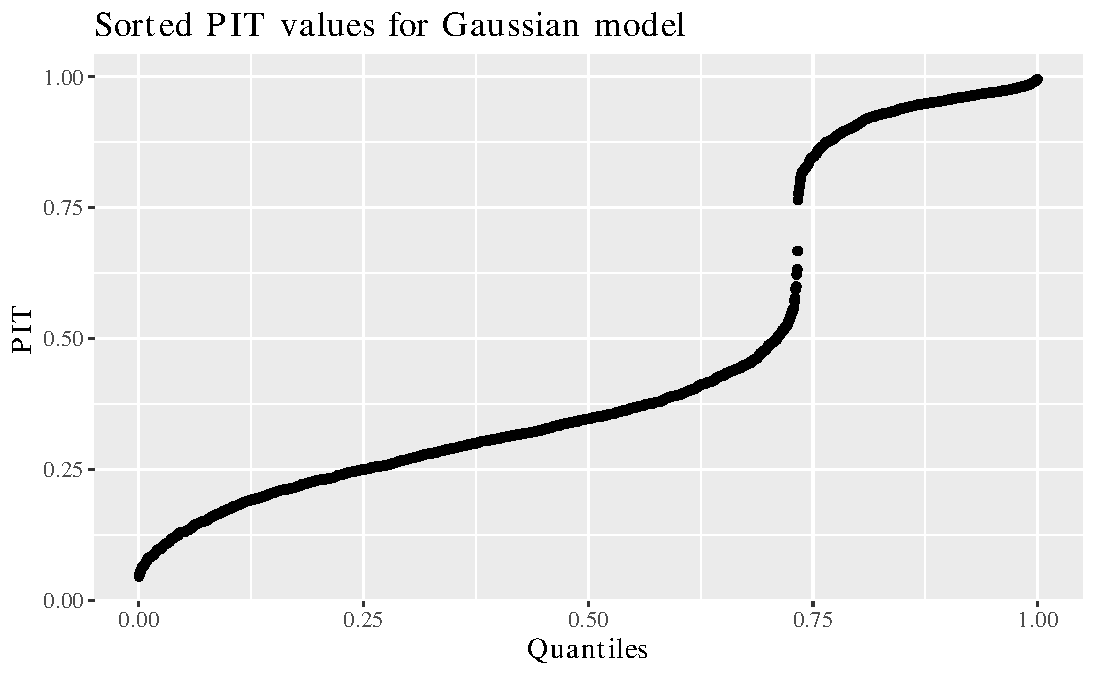
\includegraphics[width=0.8\textwidth]{figures/PIT-sorted.pdf}
    \caption{Sorted PIT values over quantiles in Gaussian application model.}
    \label{fig:sorted pit values}
\end{figure}

\begin{figure}
    \centering
    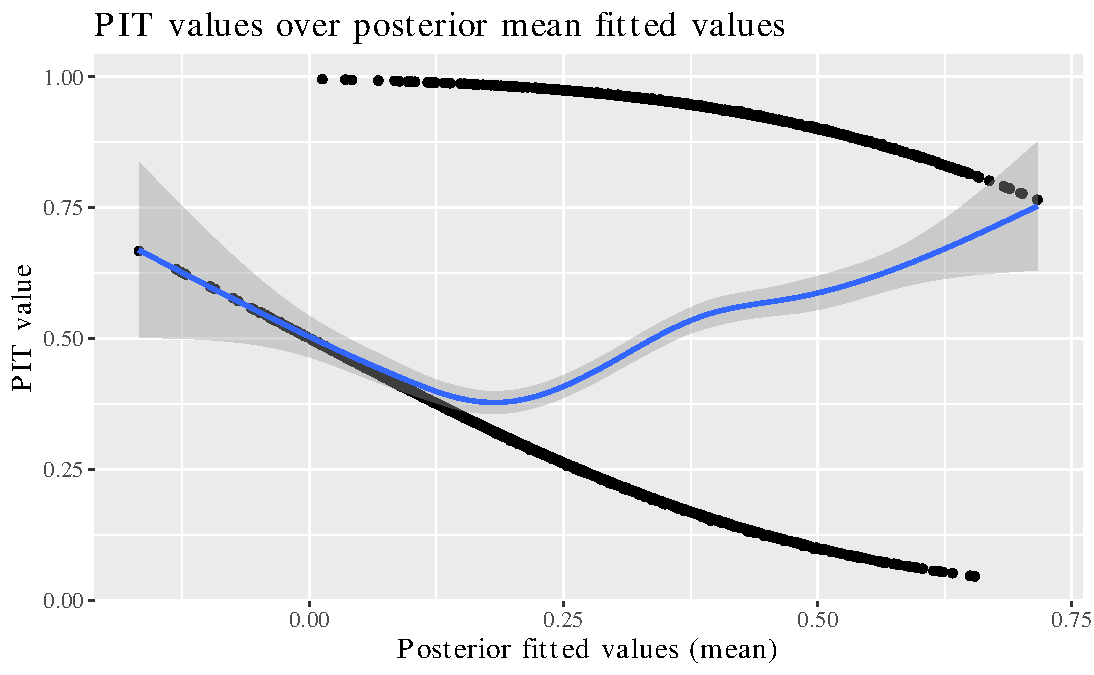
\includegraphics[width=0.8\textwidth]{figures/PIT-over-fitted.pdf}
    \caption[Gaussian model PIT vs fitted values in application]{PIT values over the mean of the posterior fitted values, using application data. The black dots are the PIT values, the blue line is a cubic spline smoothing and the grey area shows its 95\% confidence interval.}
    \label{fig:gaussian pit vs fitted}
\end{figure}

\begin{figure}
    \centering
    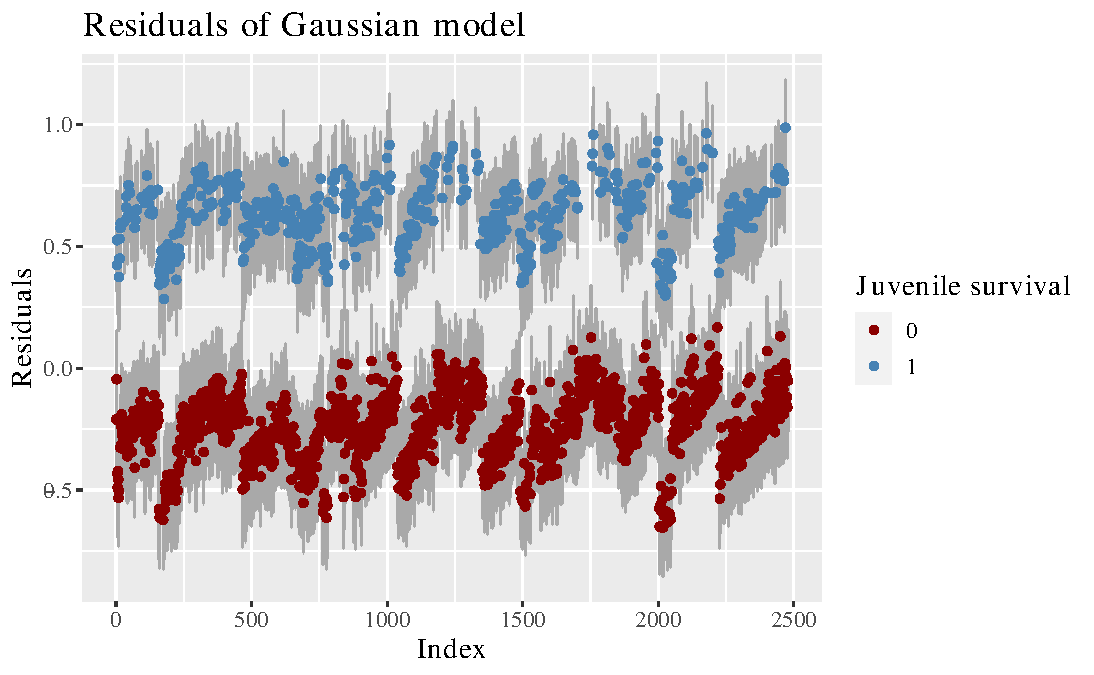
\includegraphics[width=0.8\textwidth]{figures/Residuals-gaussian.pdf}
    \caption[Residuals in Gaussian model, using simulation data]{Residuals of the Gaussian model with the song sparrow data. That is, $y_i-\hat y_i$ for all observed $i$. The blue-colored dots resemble the difference between the mean of the fitted values and the true observation where juvenile survival is true. Similarly, the red dots are when the trait is false (not survived). The dark grey lines are the 95\% credible intervals for each of the residuals, based on the quantiles computes from the posterior fitted values.}
    \label{fig:gaussian residuals}
\end{figure}

\begin{figure}
  \centering
  \begin{subfigure}[b]{0.5\textwidth}
    \centering
    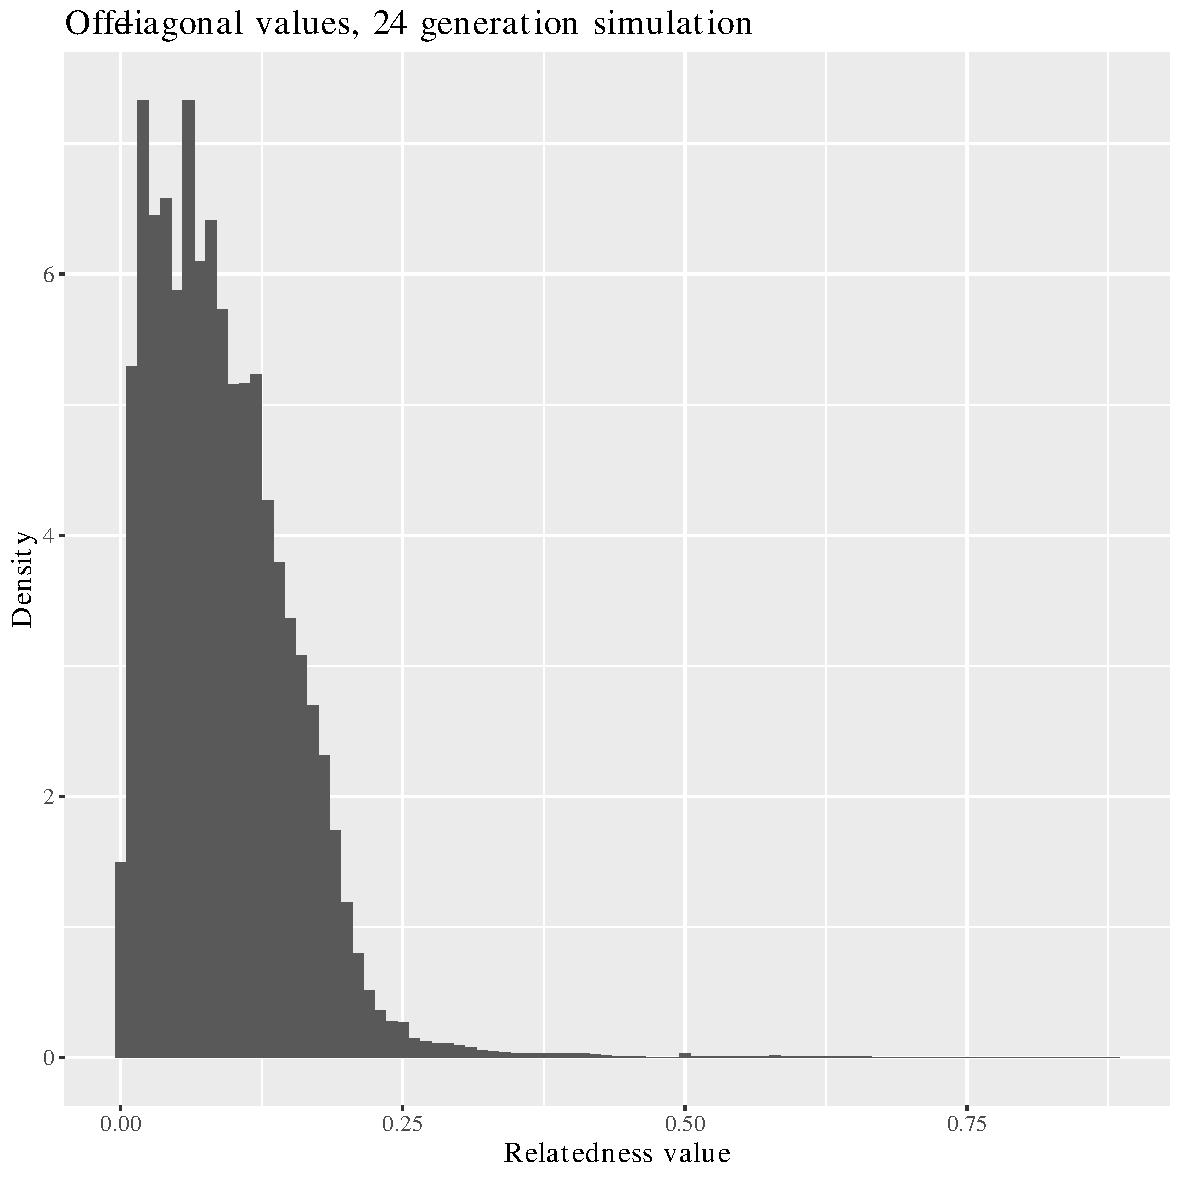
\includegraphics[width=\textwidth]{figures/relatedness-offdiagonal-sim.pdf}
    \caption{Simulation data}
    \label{fig:relatedness:simulation}
  \end{subfigure}%
  \begin{subfigure}[b]{0.5\textwidth}
    \centering
    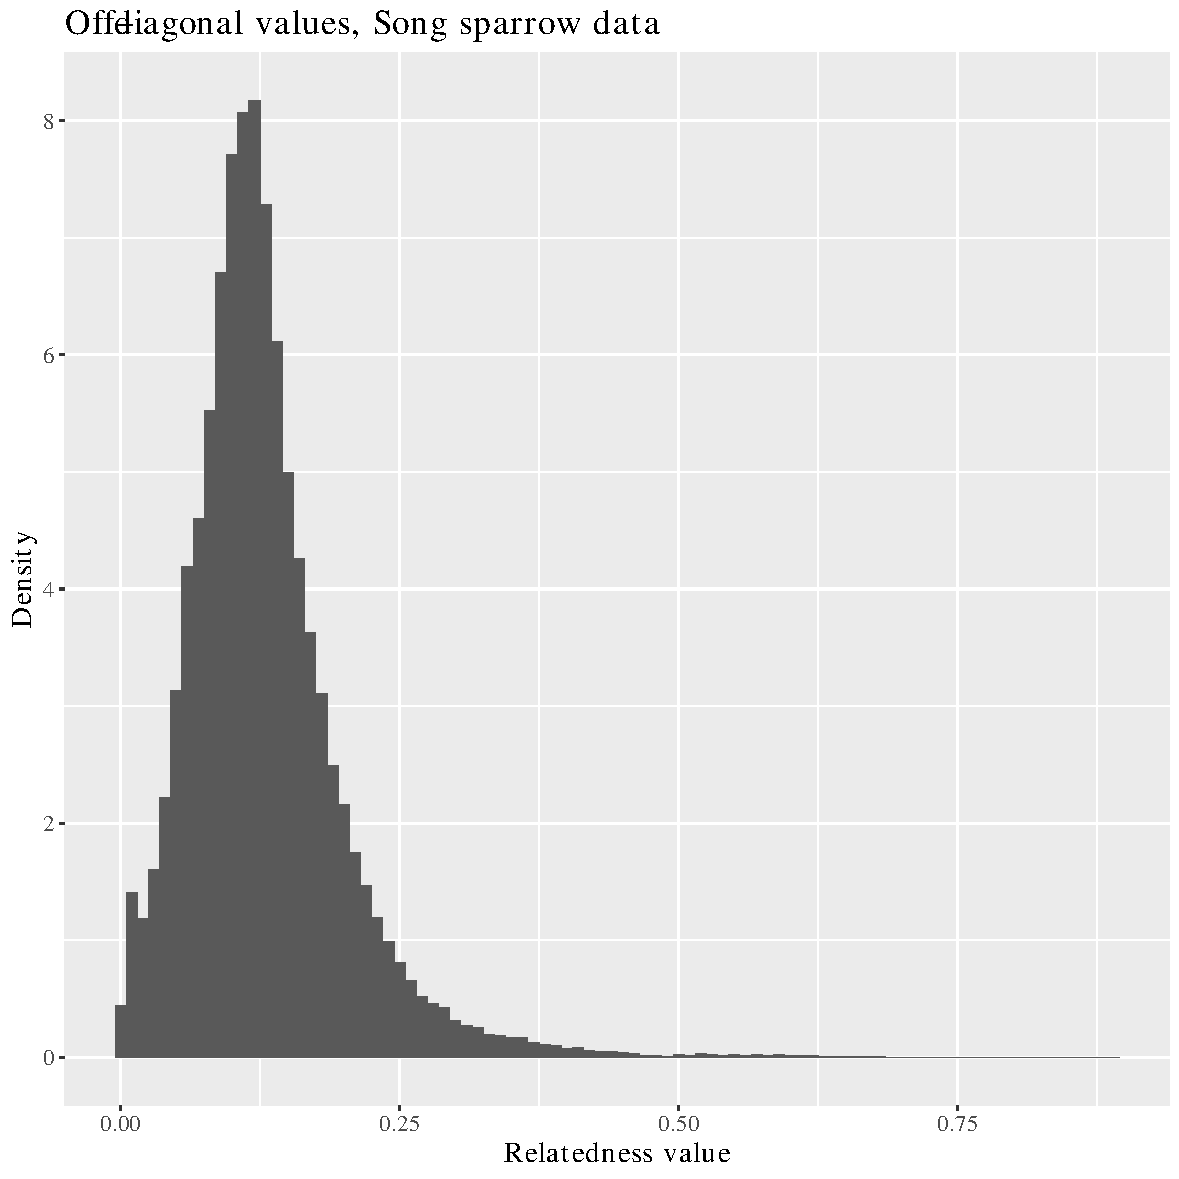
\includegraphics[width=\textwidth]{figures/relatedness-offdiagonal-songsparrow.pdf}
    \caption{Song Sparrow data}
    \label{fig:relatedness:realdata}
  \end{subfigure}
  \caption[Off-diagonal values in simulated relatedness matrix]{Histograms showing the density of the different relatedness values in the relatedness matrix for the simulation data, and the song sparrow data, respectively. The diagonal values (measuring relatedness to the individual itself) are not included, as self-relatedness is one by construction.}
  \label{fig:relatedness offdiagonal}
\end{figure}
\chapter{Discussion} \label{sec:discussion}
The present discussion chapter aims to provide a critical review and comparison of the different scales of heritability estimates obtained using the different models. The results in the previous chapter provide the basis for discussion, where we specifically will evaluate the validity of the Gaussian model, its computational aspects, and whether a Gaussian model can be sufficient for heritability estimation. Included in the chapter is a section on future potential work in the same research domain. 

%% The following didn't fit anywhere...
% \textcite{reid2021} concluded that the additive genetic variance, $\sigma^2_A$ was either overestimated, or potentially something else contributes to decreased the mean phenotypic value. This because we're measuring juvnile survival which is very related to fitness.

\section{Gaussian estimates in simulation}
The overall results in \autoref{fig:simulation_h2_dev} show that the scaled heritability from the Gaussian model coincides well with the true heritability on the underlying scale. For lower values of $\sigma^2_A$ and hence $h^2$ (\autoref{fig:simulation_h2_dev:small}), both the scaled and unscaled plots seem to be close. However, when $h^2$ increases, it becomes more apparent that we need the threshold scaling.

One potential problematic component of the model specification in the simulation case is the choice of priors. In the model, the prior is chosen based on the true value for $\sigma^2_A$, ensuring a well-suited prior estimate. However, this may not reflect the degree of prior knowledge in most datasets, especially not in wild population surveys. To challenge this prior assumption, we performed two different simulations: one with a constant PC prior PC$(1,0.05)$ for all $\sigma^2_A$, and one case with PC$(U, 0.05)$ with $U=2\sigma^2_A$. Both simulations yielded results very similar to the varying priors explained in the methods chapter. % Another thing that may influence the performance of INLA-fitted models, is if we use full Laplace approximation or simplified Laplace approximation (see subsection 3.3.1). \autoref{sec:method:inla}.
Furthermore, we can also note that the binomial dichotomization shown in \autoref{fig:simulation_h2_dev:binom} seems to somewhat underestimate the underlying heritability, compared to the threshold dichotomization. The dichotomized values in this case are binomial realizations with success probability given by applying the normal cumulative density function ($\Phi$) to $\Tilde{\bm\eta}$, and this dichotomization choice introduces variance that would explain this result. One way to consider the introduced variance from binomial dichotomization is that the mapping from an underlying Gaussian distribution onto the binary traits is not exact and contributes to some unexplained variability. Thus, binomial dichotomization can represent the same as including residual variance in the denominator.
% For the latter case with rounding, we can quite easily obtain the variance introduced by rounding. Assuming that $\Tilde{\eta} \sim \mathcal N(0, \sigma^2)$ for an arbitrary $\sigma^2$, we define $v$ such that
% \begin{equation}
% v = 
% \begin{cases}
%     0, \quad \Tilde{\eta}\le0,\\
%     1,\quad \Tilde{\eta} > 0
% \end{cases} .
% \end{equation}
% Then,
% \begin{align}
% \operatorname{E}[v] &= 0 \cdot \operatorname{Pr}(v=0) + 1\cdot \operatorname{Pr}(v=1) \\
% &= \operatorname{Pr}(\Tilde{\eta}>0) \nonumber \\ 
% &= 1-\operatorname{Pr}(\Tilde{\eta}/\sigma \le0) \nonumber \\
% &=1-\Phi(0)=0.5. \nonumber
% \end{align}

% The variance of $v$ becomes
% \begin{align}
% \operatorname{Var}[v] &=\operatorname{E}[\left(v-\operatorname{E}(v)\right)^2] \\
% &=\operatorname{Pr}(v=0)(0-0.5)^2+\operatorname{Pr}(v=1)(1-0.5)^2 \nonumber\\
% &=0.25\quad\forall \sigma^2, \nonumber 
% \end{align}
% \todo{Unsure about the relevance of these computations.}
% which indicates that using rounding, although it introduces some dichotomization variance, should not be the source of any significant error in the simulation study.

\section{Interpretability on different scales}
%%% Part 2 of thesis discussion
This section will consider how the heritabilities obtained from the different scales relate to each other, aiming to answer whether one can use Gaussian regression instead of binomial regression. Recall that a summary of the different scales is provided in \autoref{tab:h2 notation}.

The first result to consider is the mean and mode of posterior heritability (Tables \ref{tab:heritability simulation} and \ref{tab:heritability application}). The means and modes have relatively little skewness, since the mean and mode are close to each other, although the mode is consistently lower than its corresponding mean. This can be attributed to some small positive skewness in all of the models.

We may also note that for the application data, the Gaussian $h^2_\text{obs}$ is less than one standard deviation away from the corresponding probit models on the observation scale, $h^2_\Psi$ and $h^2_\Phi$. The simulation data become more challenging to interpret. The underlying heritability would in our case be $0.5/(1+0.5)=\frac13$, assuming it follows a Gaussian distribution before dichotomization. In this case, the heritability from the Gaussian model transformed to the liability scale $h^2_\text{liab}$, along with the link variance transformation $h^2_\Phi$, provides estimates closest to the true value (see \autoref{tab:heritability simulation}). This is in line with what we expected, as the two heritability estimates have the same liability scale, whereas the others are on a different scale. Furthermore, solving for the theoretical $h^2_\text{obs}$ using the threshold model and the true value for $h^2_\text{liab}$, we obtain with the simulated $\hat p=0.46$, that the true heritability of the observation scale would be $0.211$.

As expected, the Gaussian $h^2_\text{obs}$ and binomial back-transformed $h^2_\Psi$ are the closest, where the binomial model's mode is, to a small degree, closer to the true value than the Gaussian mode (\autoref{tab:heritability simulation}). Hence, it seems that the Gaussian model overestimates heritability, albeit to a small degree.
%Note that in the context of the simulation study, the latent scale heritability is found to be very close to $1$. This can be attributed to the presence of only two random effects, namely the breeding value and an iid random effect, which is estimated to be close to zero.

The figures supporting the heritability estimates from the tables are the figures of its posterior density (Figures \ref{fig:posterior simulation heritability} and \ref{fig:posterior application heritability}). Recall that $h^2_\Psi$ is more computationally intensive but also more precise than $h^2_\Phi$, which motivates comparing the precise $h^2_\Psi$ to the Gaussian model instead of $h^2_\Phi$. In addition, the liability scale for the Gaussian model should be equivalent to $h^2_\Phi$ \autocite{de2016general}.

Observing first the observation scale (Figures \ref{fig:posterior simulation heritability:observation} and \ref{fig:posterior application heritability:observation}), we can instantly remark that $h^2_\text{obs}$ and $h^2_{\Psi}$ are very similar. The Gaussian estimate is more positively skewed for the application data, but is generally very similar to $h^2_\Psi$ in terms of shape and numerical values. The simulation has a larger deviation between modes, as the probit one seems to be shifted towards the right. This is in line with our observations from the table summary. The liability scale for the Gaussian model is compared with $h^2_\Phi$ (Figures \ref{fig:posterior simulation heritability:liability} and \ref{fig:posterior application heritability:liability}), where we observe similar deviations, though with less skewness for the Gaussian model.

\subsection{Robustness of the models}

Robustness tests provide information on the performance of various models in estimating heritability on different scales. Based on the fixed effect Gaussian models for varying $\sigma^2_A$ (\autoref{fig:fixed effects sim deviance gaussian model}), the Gaussian model obtains estimates of underlying heritability that somewhat approximate the theoretical true value for a balanced phenotypic mean. However, heritability appears to be overestimated, especially in the case of an unbalanced phenotypic mean. Thus, it seems like the threshold model breaks down with a dominating fixed effect.

Additionally, the posterior density of heritability on the observation scale (\autoref{fig:fixedeffects probit vs gaussian}) suggests that both the binomial and Gaussian models struggle to accurately estimate heritability on the observation scale when a fixed effect dominates the linear predictor. In general, it is difficult to determine whether the back-transformed probit or the Gaussian model is the closest to the correct value in this result, as we have no true observation-scale heritability for reference. The true heritability (based on the chosen values for the other components of the linear predictor) is on a liability scale, and we cannot safely state that $\hat p$, the estimator for the marginal phenotypic mean $p$, is sufficient to approximate each conditional $p_i$. Recall that each dichotomized $y_i$ has its underlying probability $p_i$ and is dependent on the covariate for each individual $i$.

The difference between heritability from the back-transformed probit and Gaussian models appears to also be apparent in larger values of $\sigma^2_A$, though to a smaller degree with a balanced phenotypic mean (Figures \ref{fig:fixedeffects probit vs gaussian:hVAlP} and \ref{fig:fixedeffects probit vs gaussian:hVAhP}). When the magnitude of $\beta_\text{sex}$ for the fixed effect decreases, the proportion of total variance from fixed effects becomes smaller, meaning that we would expect the two heritability densities to be closer to the same value, which is confirmed in \autoref{fig:fixedeffects varying betas} in the appendix.

An important aspect that may explain the results is that the simulation only has one single, binary, and dominating fixed effect. As a consequence, the individual's response is directly associated with its covariate for the fixed effect. Had we used more fixed effects, effects with a smaller weight $\beta$ and perhaps continuous covariates, the inclusion of fixed effects may not lead to the same results as we have in our simulations. Supporting this idea are the results from the simulation work where the model uses several fixed effects, where the Gaussian model obtains heritability estimates close to the probit model with back-transformation (\autoref{fig:posterior application heritability}).

% In this figure, the probit model performs better for smaller heritability and hence small $\sigma^2_A$, whereas the Gaussian model is in some cases better for higher heritability values, particularly when the variance is around 500 or above (see \autoref{fig:posteriors fixed simulation} in the appendix). Furthermore, the distinct difference between the back-transformed probit model and the Gaussian model we see is not as apparent in either the simpler simulation cases or the application data with a series of fixed and random effects. A more detailed analysis of how much the variance in the simulation data's fixed effects predictors may be the next line of action to further understand this result. \todo{This par must be fixed}

% This is also difficult to clearly discuss, as different runs with the same variance settings can generate significantly different results. Regardless of run, the theoretical value seems to be between the mode from the binomial model as a lower limit, and the mode of the Gaussian one as an upper limit. 

The second aspect of robustness concerns overdispersion, and the results are provided in \autoref{fig:overdisperion plots}. However, the alternative probit model without any random iid effect results in almost exactly the same posterior density as a standard probit model (with an iid effect), for all combinations tested of $\sigma^2_A$ and $\sigma^2_E$. This indicates that the model with an iid parameter sends the iid parameter towards zero and attributes the overdispersion variance to the additive genetic variance instead. In the general simulation runs, we also include an iid term, where we see that $h^2_\text{lat}$ is very close to one, indicating that the iid effect goes towards zero for simulations as well. Although the probit model does not differ when including an iid term in its linear predictor, the Gaussian model generates observation-level heritability closely resembling the probit models for the four combinations of $\sigma^2_A$ and $\sigma^2_E$.

\section{Normality of Gaussian model}
%%% Normality of Gaussian model
The normality tests of the Gaussian model indicate that the residuals are far from normally distributed, clearly violating the model assumptions of a linear model (Figures \ref{fig:sorted pit values} to \ref{fig:gaussian residuals}). Violation of the model assumptions has consequences for further model inference, since, for example, the F-test is sensitive to the normal assumption \autocite{f-test-normality}. In general, models that violate their assumptions can also lead to more biased estimates, since the predictor in linear regression assumes Gaussian residuals with constant variance. If the residuals no longer have constant variance, the equivalence between the closed form solution \eqref{eq:theory:closed form linreg} and the maximum likelihood estimate also becomes violated. Thus, the estimates from the predictor and consequently variance and heritability estimates can also be subject to bias. This clear violation is here, however, expected, seeing as the model fits a binary phenotype as the response.

Another result in favor of using binomial regression is the deviance information criterion whose values are shown in Tables \ref{tab:simulation DICs} and \ref{tab:application DICs}. In both datasets, the binomial model has a significantly lower DIC value than the Gaussian equivalent. Note that we cannot compare DIC values across different datasets, as they should only be used in model selection. Thus, varying values between probit models for the different datasets are expected, and we cannot infer any conclusions from such a result.

Despite clear violations, we still see overall good performance from the Gaussian model. Therefore, the bias to additive genetic variance introduced by normality violation may not be severe enough to bias heritability. Since heritability is a ratio between variances, another possibility would be that the bias in $\sigma^2_A$ is somewhat counteracted by taking the ratio of total phenotypic and additive variance. These hypotheses are difficult to test for but can explain why the heritability bias in the Gaussian model is not larger. 

\section{Computational aspects}

%%% QGglmm with or without the predict argument
An important result highlighted in the back-transformation techniques on the application data (\autoref{fig:qgglmm application}), is that the simpler, yet faster method \textit{No averaging} yields results strikingly similar to the two slower methods averaging over fixed effects. Estimates deviate significantly more in the simulation case (\autoref{fig:qgglmm simulation}) when using a larger additive genetic variance.

As shown by the execution time of the methods in seconds (\autoref{tab:h2psi runtime}), the fastest technique (\textit{No averaging}) is more than six times faster than the most computationally demanding (\textit{Bayesian}). In the specific case of a binary probit model, the algorithm does not require numerical integration, meaning that all methods are sufficiently fast and we can use the method denoted by \textit{Bayesian}. If we had considered other link functions without a closed form back-transformation such as the logit link, the fastest method might be the only viable choice.

In general, the choice of fixed effects is expected to substantially change the heritability estimate \autocite{wilson2008}, in line with the results of the simulation with sufficiently high $\sigma^2_A$, but contradictory to our results for the application data. We fit our models in a Bayesian statistical context, and other modeling frameworks can yield different results. In addition, \textcite{qgglmmguide2020} shows a case study in which averaging changes the observation-scale heritability from about $0.3$ without averaging, to $0.2$ with averaging. Thus, we cannot state that one does not need the process of averaging over fixed effects in general. The results also show that for sufficiently large $\sigma^2_A$, the different densities of $h^2_\Psi$ will deviate more from one another (\autoref{fig:qgglmm simulation:bigvA}). Lastly, we have not tested different values for the hyperparameter $w$, the integration width in \autoref{alg:qgglmm}. With a smaller $w$, the integrals are evaluated over a smaller space, which would yield more accurate results assuming it would not increase the numerical integration error. However, for the case of binary probit, $w$ is not used and thus is not taken into account.                    

\section{Further work}
The robustness tests indicate that including fixed effects in the denominator may be appropriate. However, the tests do not clarify which cases it is necessary to include variance from fixed effects, seeing as the application data provides accurate estimates without including variance from fixed effect in the heritability estimation. Another shortcoming of the findings is to what extent we can generalize the results of the robustness tests. Although we have tested some extensions, the simulation datasets do not introduce complex animal models with several fixed effects. An alternative approach would be to fit two animal models without fixed effects, one with the data for $\bm x_\text{sex}=0$, and the latter with $\bm x_\text{sex}=1$. Then, one would expect, for a sufficiently large sample size, that the heritability would be similar.

Another aspect worth considering is modeling with a more unbalanced response variable. For example, looking at models whose binary trait is highly unbalanced ($p < 0.1$), could provide insight into limitations to the Gaussian model, as suggested in \textcite{vanvleck1972}. Furthermore, some animal models may also have generous use of interaction terms in the model statements, which has neither been discussed nor included in this thesis.
Also, note that a deliberate limit in the thesis was made by assuming that heritability is the most important metric when analyzing wild populations. However, heritability has been subject to scrutiny and some claim that other measurements related to additive genetic variance can be more appropriate, such as evolvability \autocite{hansen2011}.

Finally, in wild population studies, missing data tend to be more prevalent compared to the datasets used in this thesis. For the simulation case, we have an artificially complete pedigree. For our song sparrow data, we also have a complete pedigree that is not comparable to most wild population survey data. In a further study, it could be interesting to see how missing data and sensitivity to pedigree errors can influence Gaussian heritability estimates, for instance, by applying a capture-recapture animal model \autocite{papaix2010combining}.
\chapter{Conclusion}

This thesis has explored the use of Gaussian models on binary phenotypes within the framework of the animal model and Bayesian statistics, directly obtaining observation scale heritability. The results, based on a dataset and simulation data, show that the Gaussian models can indeed be useful to easily obtain a heritability estimate, as a simpler and more direct alternative to binomial models with back-transformations. The results are limited to the datasets and models applied in the thesis and do not account for highly unbalanced phenotypes.

Furthermore, simulated data indicate that the introduction of overdispersion does not significantly challenge the Gaussian model. However, the heritability estimates from a Gaussian model diverge from the back-transformed probit model upon the introduction of fixed effects in the simulation study. Additionally, the simulation work has demonstrated that including the variance from a fixed effect in the denominator for heritability may be necessary to get an accurate heritability estimation in a Gaussian model. The models with the application data containing several fixed effects do not exhibit the same effect, and it seems like the Gaussian model provides estimates very close to the probit models' estimates. In general, using a Gaussian model also limits the use for further inference, as its general predictive abilities are significantly worse on binary phenotypes than a binomial model.

The findings show that a Gaussian mixed model is able to capture heritability on an observation scale that closely resembles the state-of-the-art back-transformation techniques for binomial models. Further investigation is required to determine exactly what effects decrease the power of a Gaussian model, although the results in this thesis indicate that it would be applicable in most practical cases. In the long term, the results can provide the foundation for developing a simpler, more effective, and easily interpretable statistical method for estimating additive genetic variance.


\chapter*{\bibname}
\begin{refcontext}[sorting=nty]
\printbibliography[heading=none]
\end{refcontext}
% Probably not relevant
%% % First paper


\appendix
% \chapter{Omitted theory}
% \label{app:theory}
% \todo{Would like feedback if this is necessary and/or a good way of including extra theory.}
% \section*{Why  $\bm Q$ is sparse in a GMRF}
% In a GMRF, we have the graph $\mathcal G = (V, E)$ with vertices $V$ and edges $E$ and the random vector $\bm X=\{x_\nu\}_{\nu \in V}$. Furthermore, $\bm X \sim \mathcal N(\bm 0,\bm Q^{-1})$ and satisfies the Markov property $x_j \perp x_{i} | x_{-ij}$, where $i$ and $j$ are not neighboring vertices in the graph, and the notation $ x_{-ij}$ are all $x_k \in \{x_\nu\}_{\nu \in V \setminus \{i,j\}}$. Thus, by construction, we get that $\bm Q_{ij}=0$, so that $\bm Q$ is sparse. 

% \section*{Genetic groups in animal models}
% We can partition the additive genetic effect into a term capturing individual variation and another capturing immigrant genes, $a_i = u_i + gq_i$. Here, $u_i$ is the deviation from $i$ to the other native group, $q_i$ is the expected contribution of immigrant genes and $g$ is an immigration coefficient, computed as the difference between the native population and the immigrants' genetic group. Notice that this means that the $u_i$ are relative to the founder population.

% % \section*{Distribution specific variance functions}
% % For instance, in a binary logit model, $\frac{e^x}{1+e^x}\left(1-\frac{e^x}{1+e^x}\right) = \frac{\partial}{\partial x}g^{-1}(x)$. For the probit case, the distribution-specific variance function is $\Phi(x)(1-\Phi(x))$.

% \section*{Decomposition of relatedness matrix}
% We also consider the decomposition $\bm A = \bm L \bm D \bm L^\top$, in which $\bm L$ is lower triangular and contains information about what genes the individual derives from its ancestors. The diagonal matrix $\bm D$ contains within-family additive genetic variance. From this decomposition, we can construct $\bm A$ with little time and memory complexity using the algorithm described in \textcite{luo1992computing}. Thus, using the pedigree we can encode relatedness into the linear predictor of the animal model. 


\chapter{Additional plots}
% An initial step is to examine the generated pedigree and in particular the relatedness of the different individuals. \autoref{fig:relatedness offdiagonal} displays the off-diagonal values of the relatedness matrices, where a high concentration around larger values would indicate a large degree of relatedness.

\begin{figure}
    \centering
    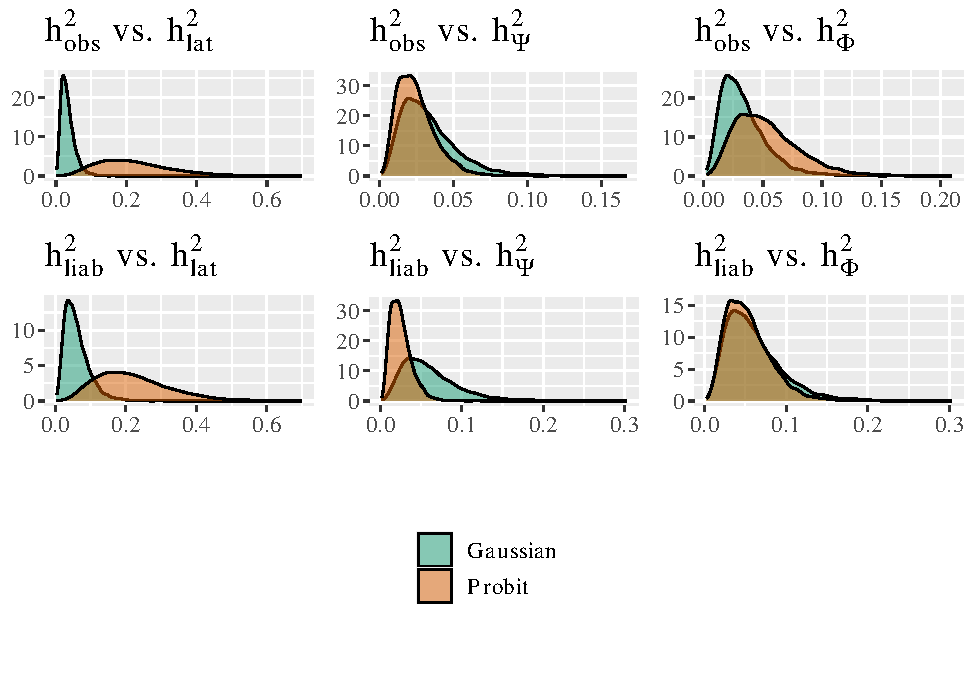
\includegraphics[width=0.8\textwidth]{figures/grid_application_gaussian_vs_binom.pdf}
    \caption[Posterior heritability for application data in different scales]{Posterior distributions of estimated heritability for the Gaussian and probit model, in the application data. The densities are reported in a grid comparing each different type of scale to each other. That is, for both scales for the Gaussian model, we compare the posterior heritability with the probit model for its three different scales. The resulting 3$\times$2 grid shows how they act comparatively.}
    \label{fig:application gaussian vs binomial}
\end{figure}

\begin{figure}
    \centering
    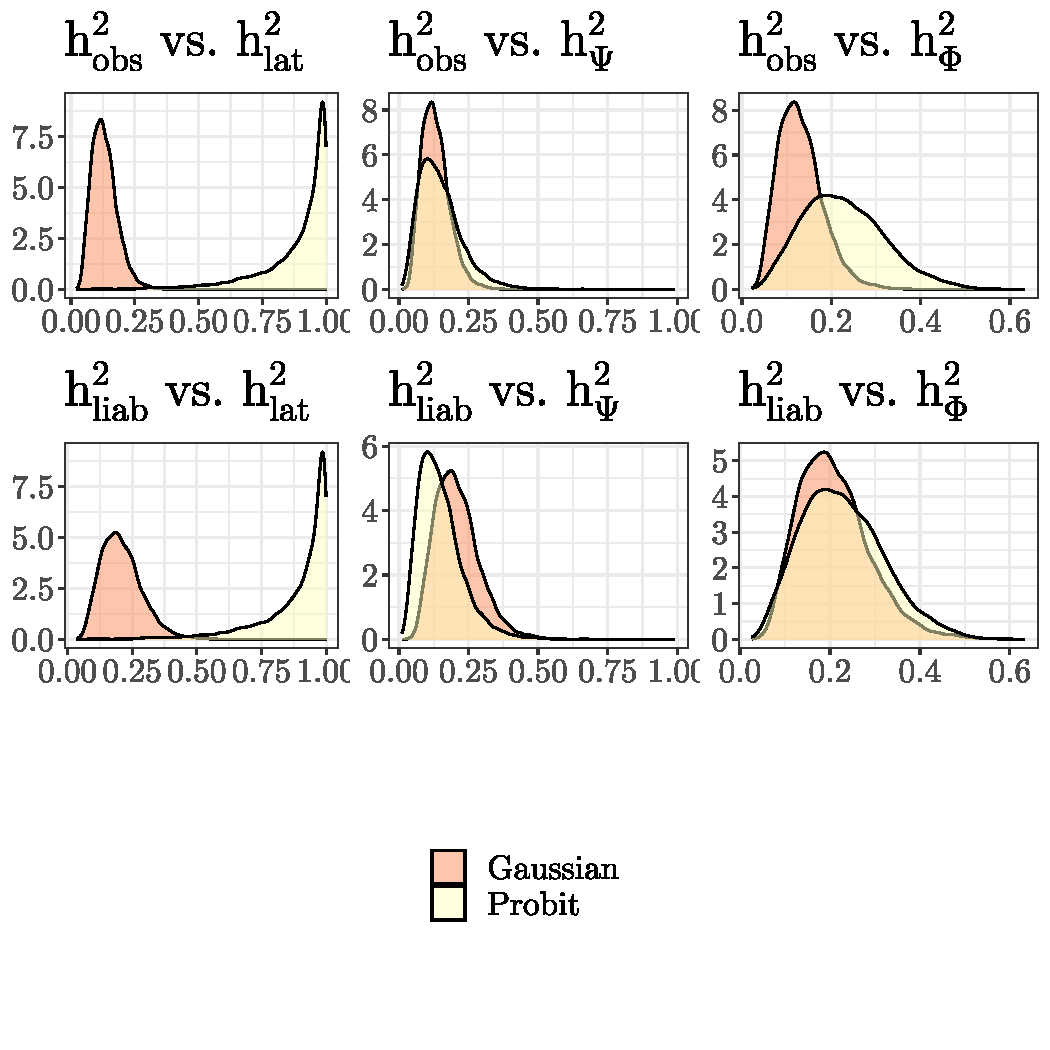
\includegraphics[width=0.8\textwidth]{figures/grid_simulation_gaussian_vs_binom.pdf}
    \caption[Posterior heritability for simulation data in different scales]{Posterior distributions of estimated heritability for the Gaussian and probit model, in the simulation data with $\sigma^2_A=0.5$ and $\sigma^2_E=1$. The densities are reported in a grid comparing each different type of scale to each other. That is, for both scales for the Gaussian model, we compare the posterior heritability with the probit model for its three different scales. The resulting 3$\times$2 grid shows how they act comparatively.}
    \label{fig:simulatino gaussian vs binomial}
\end{figure}

\begin{figure}
    \centering
    \begin{subfigure}{0.49\textwidth}
    \caption{$\beta=1$, $\sigma^2_A=10$, $\sigma^2_E=1$, $p=0.5$}
    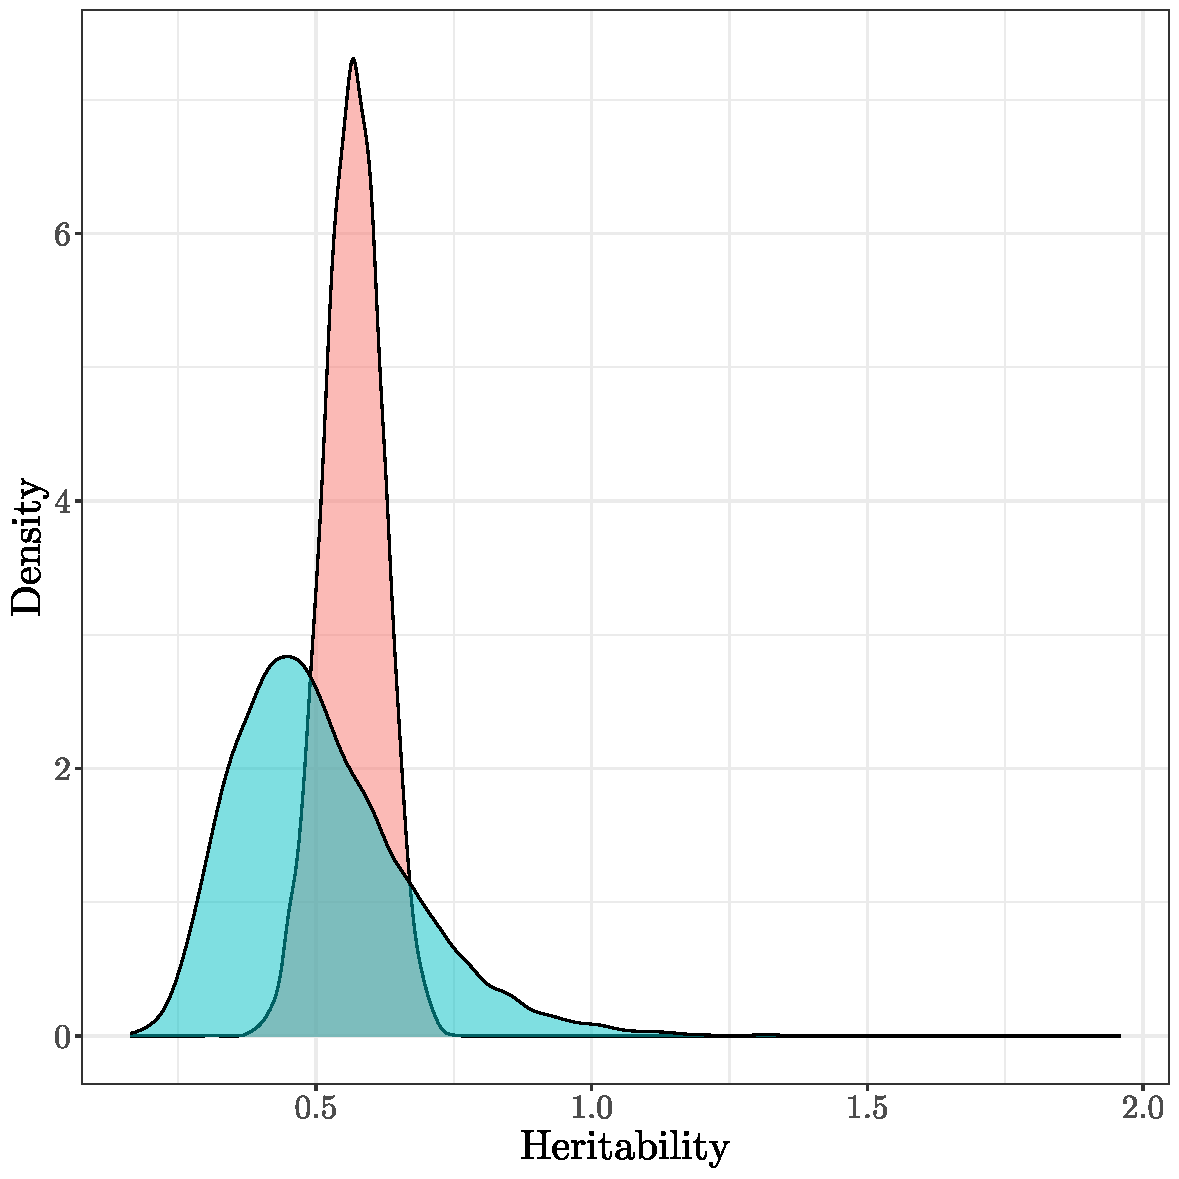
\includegraphics[width=\textwidth]{figures/fixedeffects_gaussian_probit_sA10_p_5_beta_1.pdf}
    \end{subfigure}
    \begin{subfigure}{0.49\textwidth}
    \caption{$\beta=5$, $\sigma^2_A=10$, $\sigma^2_E=1$, $p=0.5$}
    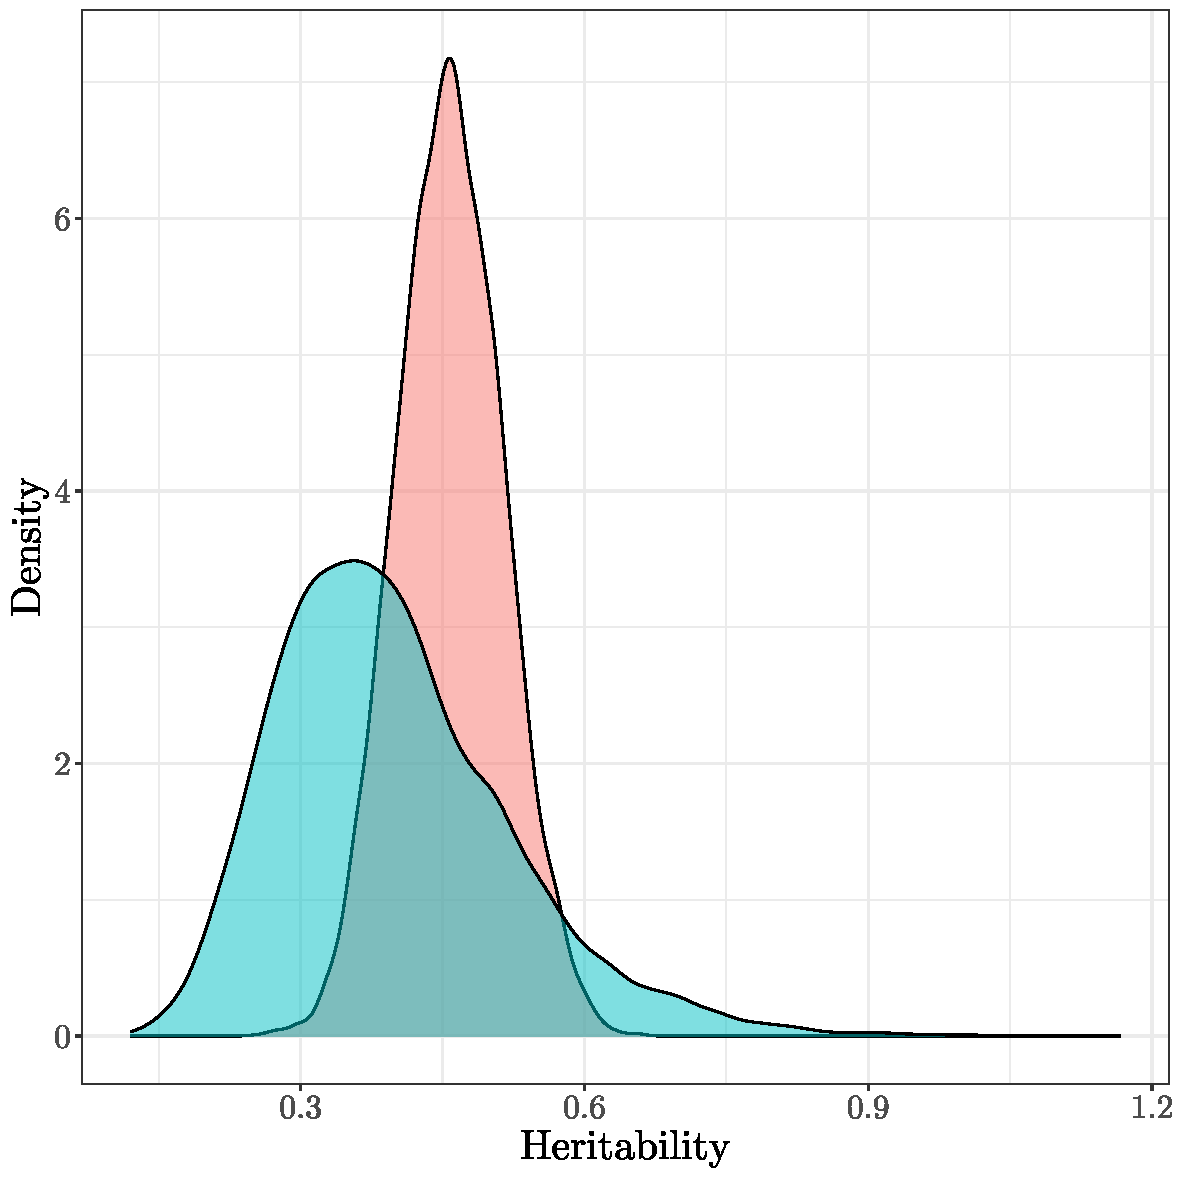
\includegraphics[width=\textwidth]{figures/fixedeffects_gaussian_probit_sA10_p_5_beta_5.pdf}
    \end{subfigure}
    \begin{subfigure}{0.49\textwidth}
    \caption{$\beta=1$, $\sigma^2_A=500$, $\sigma^2_E=1$, $p=0.5$}
    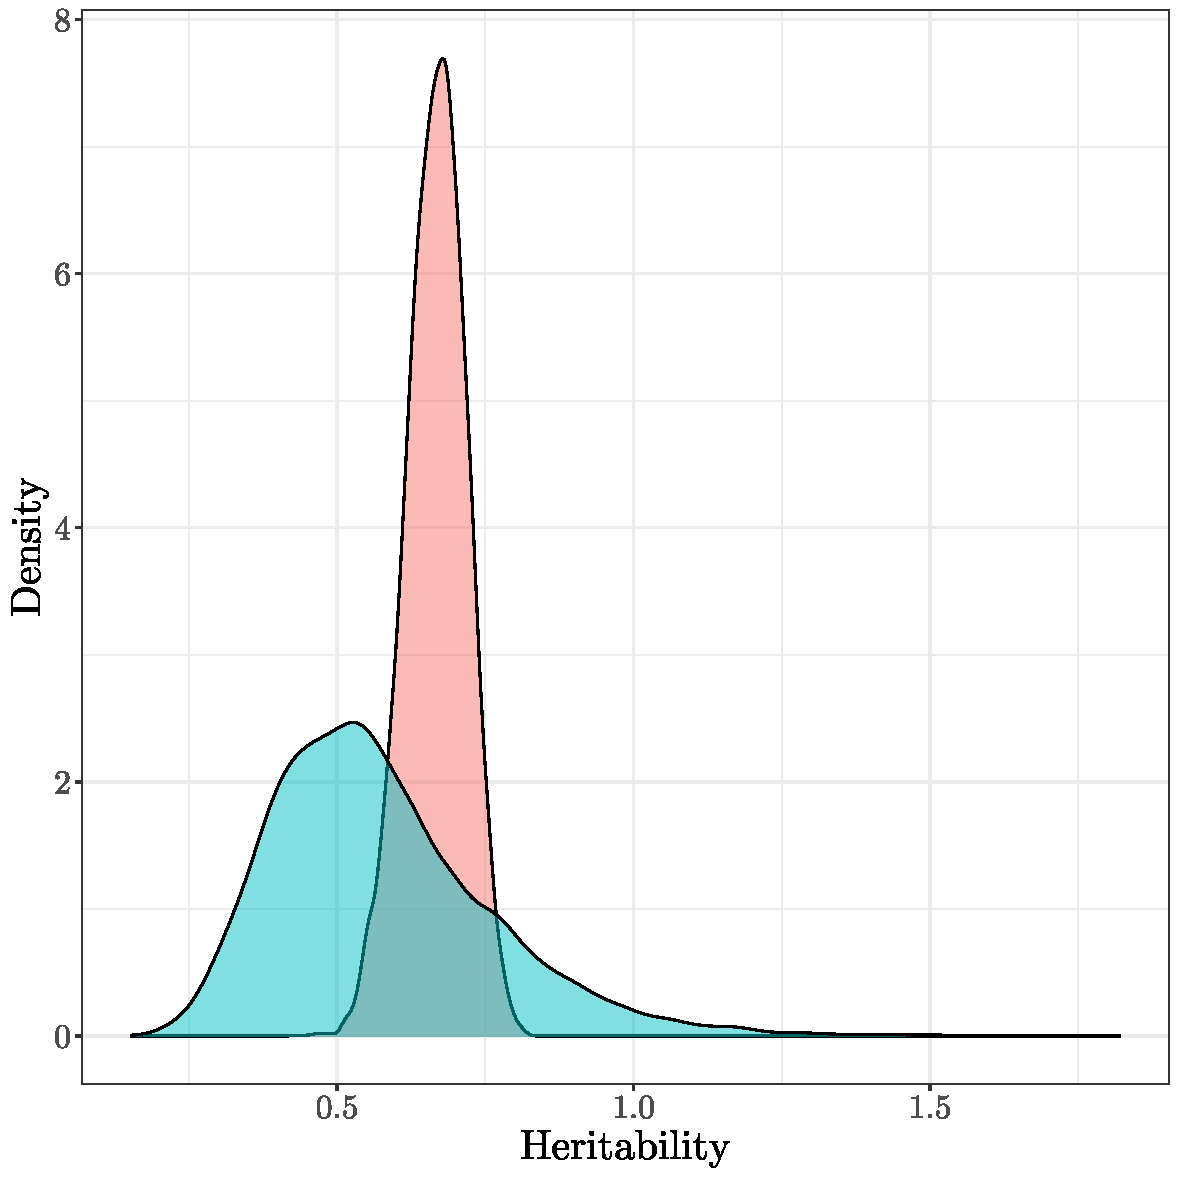
\includegraphics[width=\textwidth]{figures/fixedeffects_gaussian_probit_sA500_p_5_beta_1.pdf}
    \end{subfigure}
    \begin{subfigure}{0.49\textwidth}
    \caption{$\beta=5$, $\sigma^2_A=500$, $\sigma^2_E=1$, $p=0.5$}
    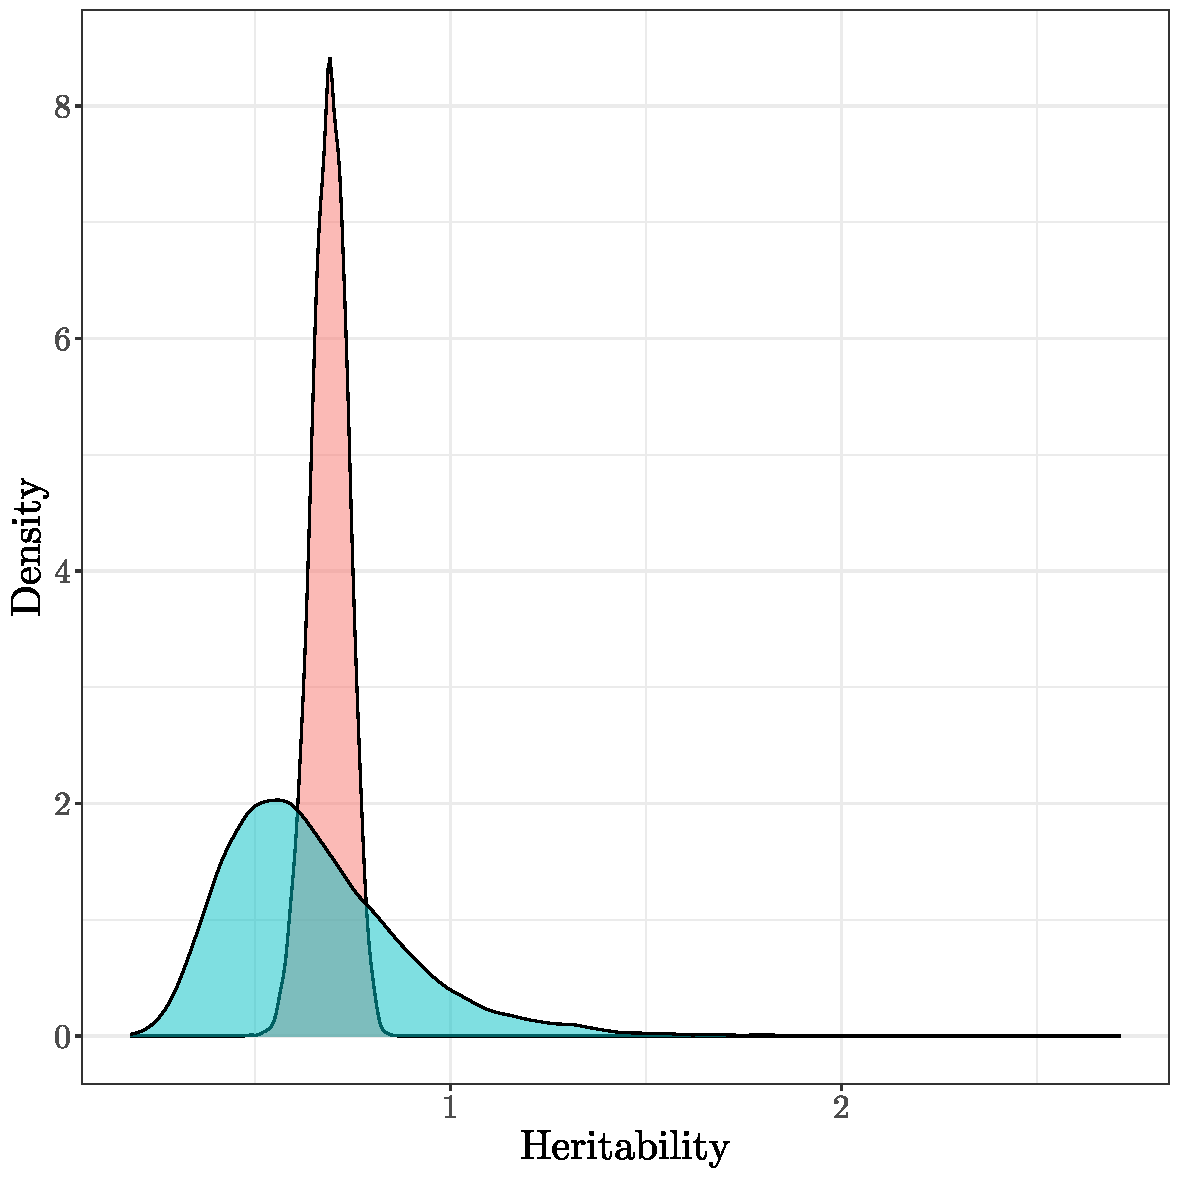
\includegraphics[width=\textwidth]{figures/fixedeffects_gaussian_probit_sA500_p_5_beta_5.pdf}
    \end{subfigure}
    \begin{subfigure}{0.6\textwidth}
    
\includegraphics[width=\textwidth]{figures/fixedeffects_gaussian_probit_legend.pdf}
    \end{subfigure}
    \caption[$h^2$ for fixed effects with varying $\beta$]{Posterior heritability for simulations with fixed effects on observation-scale, varying on $\beta$ between $1$ and $5$ across the columns, and between $\sigma^2_A=10$ and $500$ across the rows.}
    \label{fig:fixedeffects varying betas}
\end{figure}

\chapter{Exploratory Data Analysis}
\label{app:EDA}
\hypertarget{data-frame-overview}{%
\section*{Data frame overview}\label{data-frame-overview}}

\hypertarget{pedigree}{%
\subsection*{Pedigree}\label{pedigree}}

The first object is \texttt{d.ped} which contains the pedigree
information.

\begin{Shaded}
\begin{Highlighting}[]
\FunctionTok{summary}\NormalTok{(d.ped)}
\end{Highlighting}
\end{Shaded}

\begin{verbatim}
##     ninecode             gendam             gensire         
##  Min.   :109137448   Min.   :109137468   Min.   :109137448  
##  1st Qu.:146164012   1st Qu.:146130794   1st Qu.:146130313  
##  Median :176124850   Median :176124382   Median :176124004  
##  Mean   :196520240   Mean   :188116000   Mean   :185463038  
##  3rd Qu.:243185045   3rd Qu.:226189260   3rd Qu.:226189228  
##  Max.   :999999999   Max.   :999999999   Max.   :266176829  
##                      NA's   :59          NA's   :59
\end{verbatim}

It has columns \emph{ninecode}, \emph{gendam}, and \emph{gensire}.
The first column cannot be \texttt{NA} and is the unique identifier for
an individual, whereas \texttt{gendam} and \texttt{gensire} are
references (foreign keys) to the known maternal and paternal link,
respectively. Both of these columns have 59 NAs. In fact, these NAs
overlap completely since they are the founder population with no defined
paternal or maternal link:

\begin{Shaded}
\begin{Highlighting}[]
\NormalTok{d.ped[}\FunctionTok{is.na}\NormalTok{(d.ped}\SpecialCharTok{$}\NormalTok{gendam), }\StringTok{"gensire"}\NormalTok{]}
\end{Highlighting}
\end{Shaded}

\begin{verbatim}
##  [1] NA NA NA NA NA NA NA NA NA NA NA NA NA NA NA NA NA NA NA NA NA NA NA NA NA
## [26] NA NA NA NA NA NA NA NA NA NA NA NA NA NA NA NA NA NA NA NA NA NA NA NA NA
## [51] NA NA NA NA NA NA NA NA NA
\end{verbatim}

We see that \emph{gensire} is NA for all instances where \emph{gendam}
is also NA. This is the founder population with no defined parental
linkage.

\hypertarget{d.q}{%
\subsection*{d.Q}\label{d.q}}

This table has the columns \emph{g1}, \emph{foc0} and \emph{ninecode}
(ID).

\begin{Shaded}
\begin{Highlighting}[]
\FunctionTok{head}\NormalTok{(d.Q)}
\end{Highlighting}
\end{Shaded}

\begin{verbatim}
##   foc0 g1  ninecode
## 1    1  0 109137407
## 2    1  0 109137408
## 3    1  0 109137418
## 4    1  0 109137420
## 5    1  0 109137421
## 6    1  0 109137425
\end{verbatim}

Considering only the first results, it might seem like \texttt{foc0} and
\texttt{g1} are binary/categorical variables, but plotting the values
across indices show that the order of the rows are structured so that
they start at 1 and 0 respectively.

\begin{Shaded}
\begin{Highlighting}[]
\FunctionTok{par}\NormalTok{(}\AttributeTok{mfrow =} \FunctionTok{c}\NormalTok{(}\DecValTok{1}\NormalTok{, }\DecValTok{2}\NormalTok{))}
\FunctionTok{plot}\NormalTok{(d.Q}\SpecialCharTok{$}\NormalTok{g1, }\AttributeTok{main =} \StringTok{"g1"}\NormalTok{)}
\FunctionTok{plot}\NormalTok{(d.Q}\SpecialCharTok{$}\NormalTok{foc0, }\AttributeTok{main =} \StringTok{"foc0"}\NormalTok{)}
\end{Highlighting}
\end{Shaded}

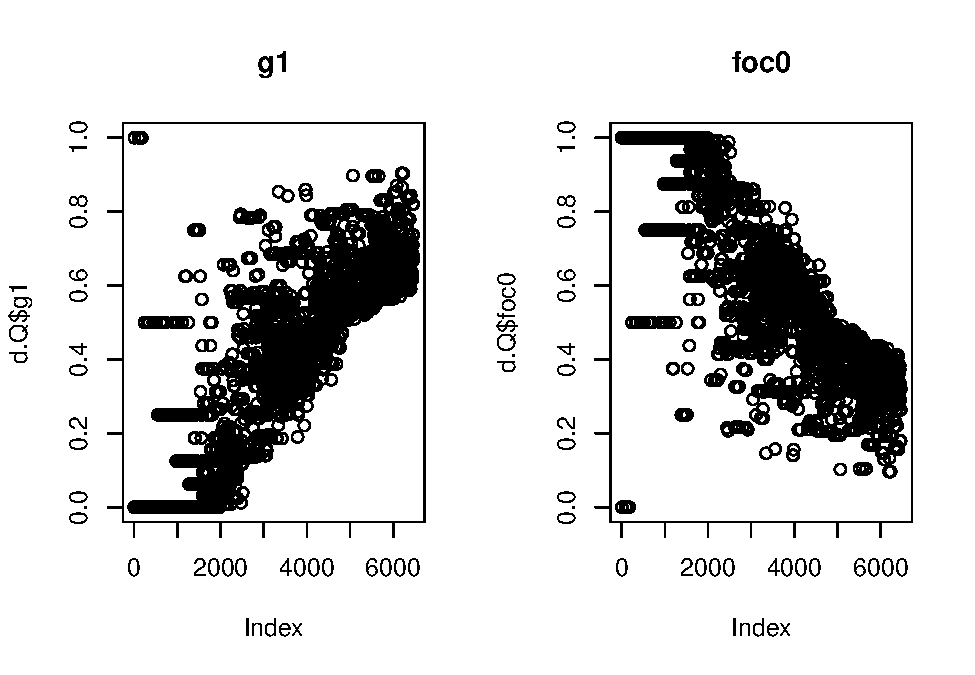
\includegraphics{EDA_files/figure-latex/unnamed-chunk-2-1.pdf}

We can also look at the correlation between these two values

\begin{Shaded}
\begin{Highlighting}[]
\FunctionTok{cor}\NormalTok{(d.Q}\SpecialCharTok{$}\NormalTok{foc0, d.Q}\SpecialCharTok{$}\NormalTok{g1)}
\end{Highlighting}
\end{Shaded}

\begin{verbatim}
## [1] -1
\end{verbatim}

Hence, we have a very strong negative correlation here. We can also look
at the individuals whose ID were in the \emph{founder population}:

\begin{Shaded}
\begin{Highlighting}[]
\NormalTok{founder\_population.id }\OtherTok{\textless{}{-}}\NormalTok{ d.ped[}\FunctionTok{is.na}\NormalTok{(d.ped}\SpecialCharTok{$}\NormalTok{gendam), }\StringTok{"ninecode"}\NormalTok{]}
\FunctionTok{table}\NormalTok{(d.Q[}\FunctionTok{which}\NormalTok{(d.Q}\SpecialCharTok{$}\NormalTok{ninecode }\SpecialCharTok{\%in\%}\NormalTok{ founder\_population.id),}
          \FunctionTok{c}\NormalTok{(}\StringTok{"foc0"}\NormalTok{, }\StringTok{"g1"}\NormalTok{)])}
\end{Highlighting}
\end{Shaded}

\begin{verbatim}
##     g1
## foc0  0  1
##    0  0 33
##    1 26  0
\end{verbatim}

The values seem to be relatively balanced between \(0\) and \(1\) in the
founder population. This supports the idea that they measure the
immigration contribution to the genetic composition of the individuals.
All immigrant individuals are completely immigrant, have no pedigree and
are thus part of the founder population. The latter are those who are
the ``initial'' natives on the island, meaning that their values must be
exactly zero.

\hypertarget{ped.prune}{%
\subsection*{ped.prune}\label{ped.prune}}

This is a pruned pedigree, only considering the 1993-2018 observations
but also combining the knowledge of the 1975-1992 observations into
them.

\hypertarget{qg.data.gg.ind}{%
\subsection*{qg.data.gg.ind}\label{qg.data.gg.ind}}

This object has the following shape:

\begin{Shaded}
\begin{Highlighting}[]
\FunctionTok{head}\NormalTok{(qg.data.gg.inds)}
\end{Highlighting}
\end{Shaded}

\begin{verbatim}
##    ninecode natalyr sex.use nestrec surv.ind.to.ad brood.date sex.use.x1
## 1 111111112    2012       0    3086              0        120          1
## 2 111111121    2015       0    3237              0        141          1
## 3 143173366    1993       1    1838              1         96          1
## 4 143173381    1993       2    1867              1        102          2
## 5 143173382    1993       1    1867              0        102          1
## 6 143173384    1993       1    1851              0        102          1
##       f.coef      foc0        g1 natalyr.no sex
## 1 0.11155218 0.4085679 0.5914321         38   0
## 2 0.04814660 0.3299752 0.6700248         41   0
## 3 0.05108643 0.5283203 0.4716797         19   0
## 4 0.03125000 0.6250000 0.3750000         19   1
## 5 0.03417969 0.4335938 0.5664062         19   0
## 6 0.02148438 0.6328125 0.3671875         19   0
\end{verbatim}

The response variable we will use is \texttt{surv.ind.to.ad}. Below are
some elementary properties of the data.

\begin{verbatim}
## [1] "Earliest year: 1993"
\end{verbatim}

\begin{verbatim}
## [1] "Number not survived: 1817" "Number survived: 661"
\end{verbatim}

\begin{verbatim}
## [1] "natal year correlation: 1"
\end{verbatim}

\begin{verbatim}
## [1] "correlation between sex and sex.x1: 0.842997540673555"
\end{verbatim}

An overview of the columns:

\begin{itemize}
\tightlist
\item
  \emph{ninecode}: Individual ID
\item
  \emph{natalyr}: The year the individual was born, e.g.~2015.
\item
  \emph{sex.use}: \textbf{Not in use}
\item
  \emph{nestrec}: ID for nest number
\item
  \emph{brood.date}: Day of the year when the first offspring in
  individuals nest hatched
\item
  \emph{sex.use.x1}: Sex of individual, 1 or 2
\item
  \emph{f.coef}: Inbreeding coefficient
\item
  \emph{foc0}: ``How foreign'' individual is, related to \texttt{f.coef}
\item
  \emph{g1}: Inverse of \emph{foc0}.
\item
  \emph{natalyr.no}: The same as the natal year, starting with 1974 as 0
  (2015=41).
\end{itemize}

\hypertarget{vizualization-of-juvenile-survival}{%
\section*{Vizualization of juvenile
survival}\label{vizualization-of-juvenile-survival}}

We will have a look at how the response, juvenile survival, relates to
the other covariates in our data.

First, we look at sex:

\begin{verbatim}
## Warning: package 'ggplot2' was built under R version 4.2.2
\end{verbatim}

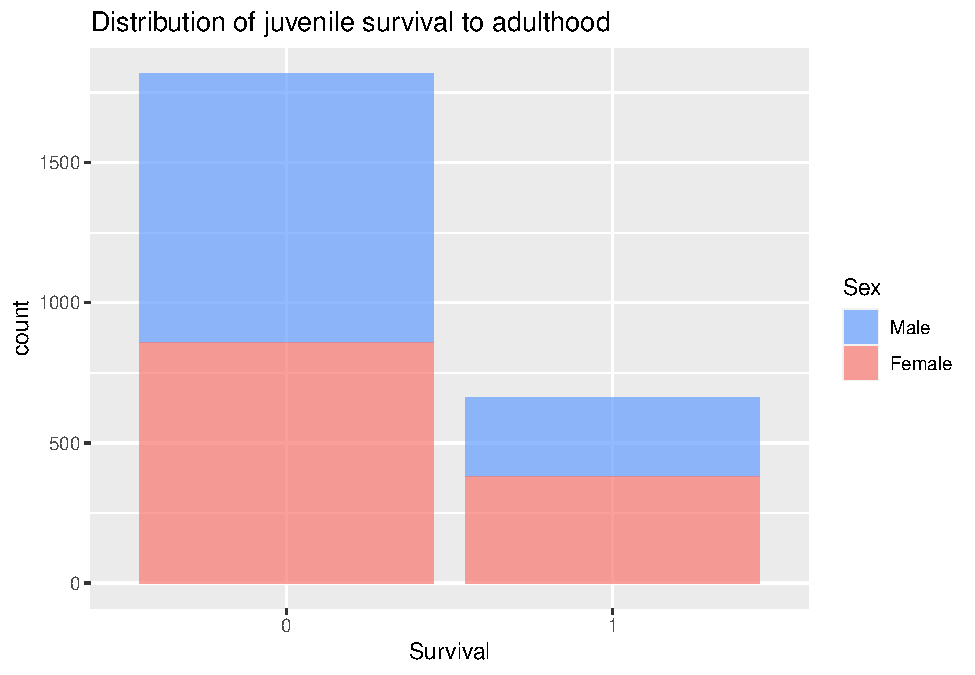
\includegraphics{EDA_files/figure-latex/unnamed-chunk-7-1.pdf}

It seems like the sex in relation to survival is relatively balanced
here. We can note that it seems like a larger portion of those surviving
are females. Next, we examine the breeding coefficient.

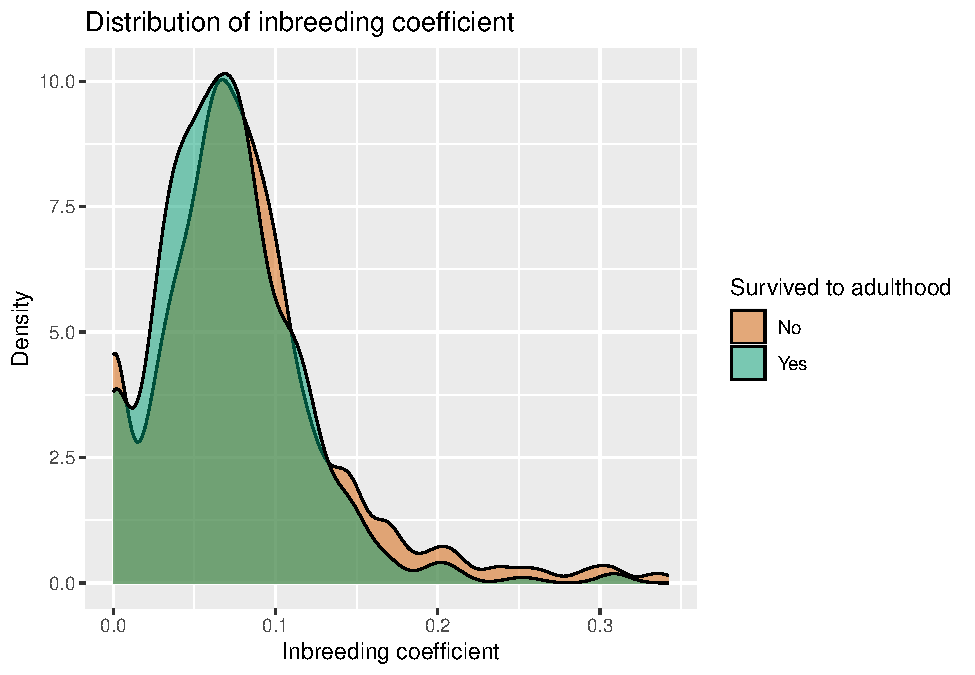
\includegraphics{EDA_files/figure-latex/unnamed-chunk-8-1.pdf}

Here we see that survival is a bit more skewed toward lower inbreeding
coefficients. We may also plot the proportion of individuals who survived
over each year:

\begin{verbatim}
## `geom_smooth()` using method = 'loess' and formula = 'y ~ x'
\end{verbatim}

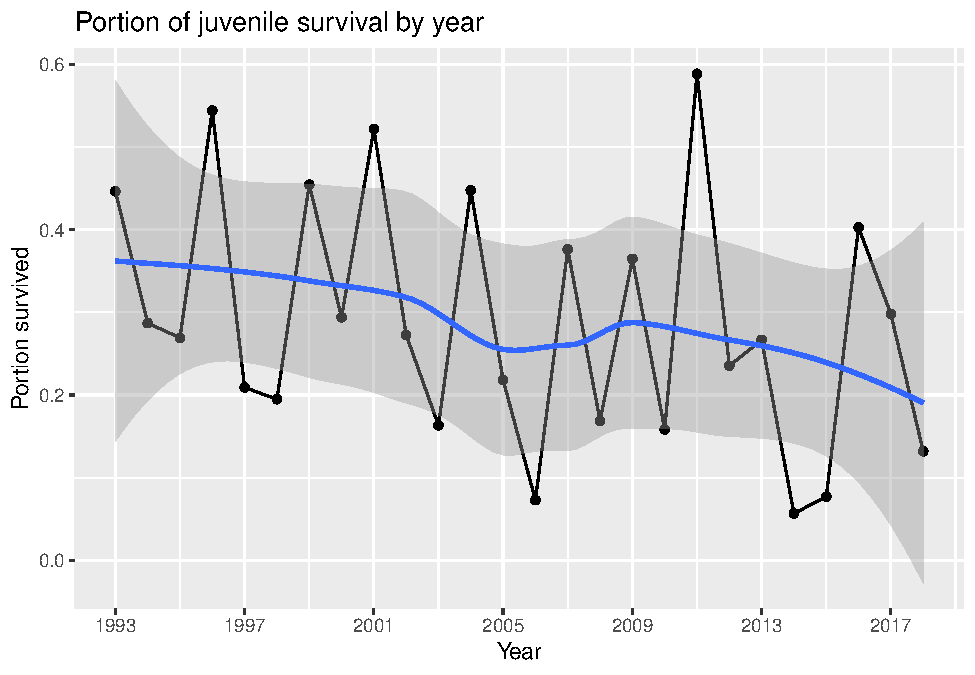
\includegraphics{EDA_files/figure-latex/unnamed-chunk-9-1.pdf}

There seems to be very little trending over the years, but possibly a
small negative trend. We also examine if there is some correspondence
between genetic group coefficient (\texttt{g1}) and juvenile survival.

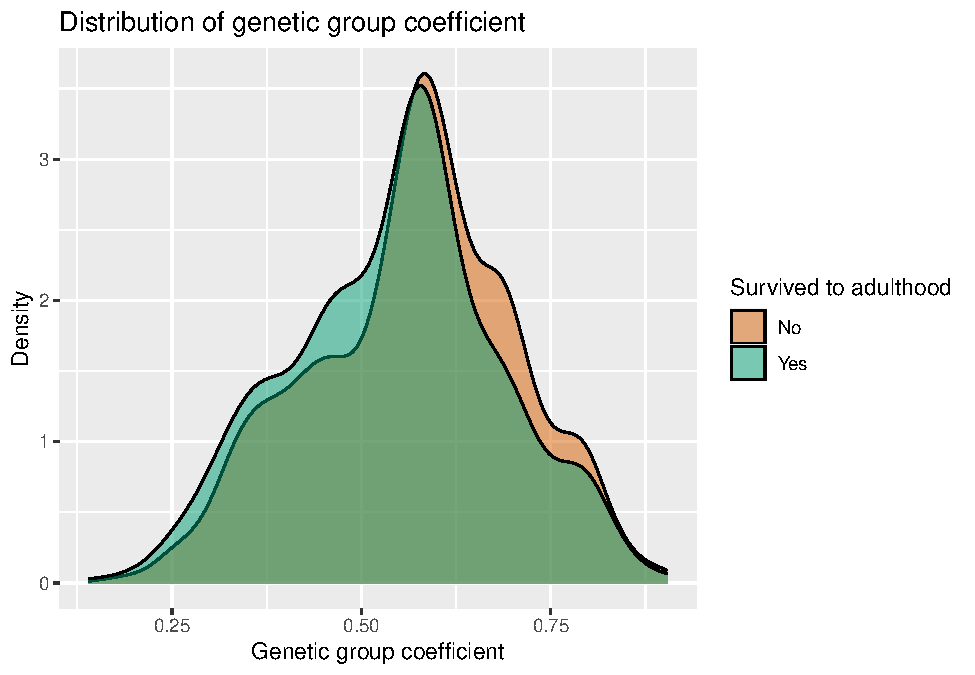
\includegraphics{EDA_files/figure-latex/unnamed-chunk-10-1.pdf}

This shows a similar result to the inbreeding coefficient, namely a skew
towards the right (lower values of coefficient) in the group that
survived. Finally, we plot the survival probability based on brood date:

\begin{verbatim}
## `geom_smooth()` using method = 'loess' and formula = 'y ~ x'
\end{verbatim}

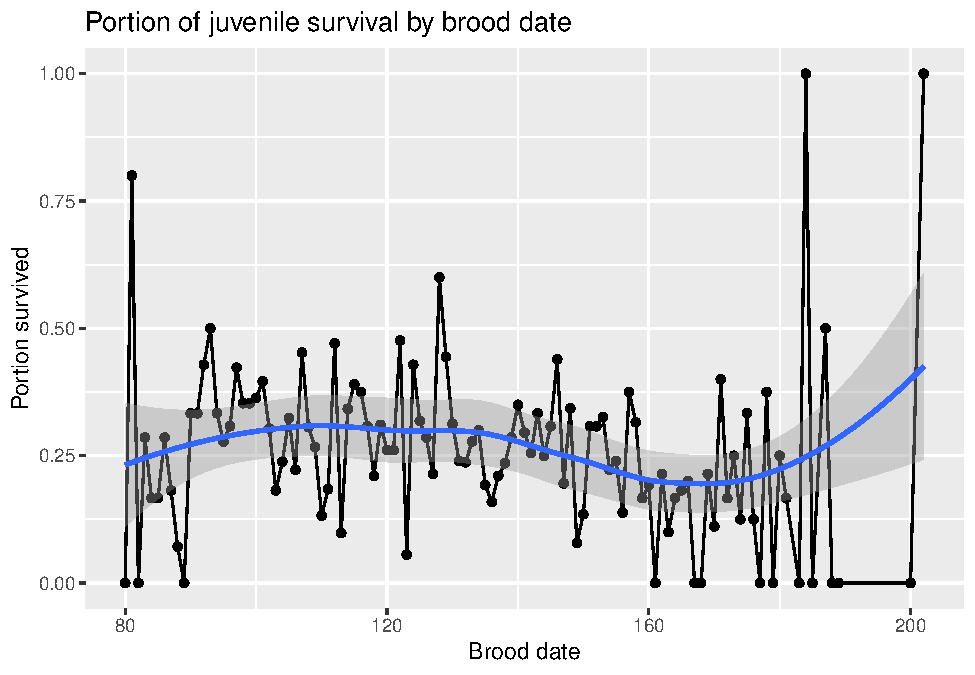
\includegraphics{EDA_files/figure-latex/unnamed-chunk-11-1.pdf}

This last plot seems to indicate that survival is relatively stable and
somewhat decreasing for those hatched relatively late. For the largest
values of brood date, we get an increasing trend but also much
uncertainty since not that many were hatched this late.

\chapter{Patching \texttt{rbv}}
\label{app:rbv-patch}
\hypertarget{how-the-bug-arises}{%
\section*{How the bug arises}\label{how-the-bug-arises}}

The function \texttt{rbv} generates random breeding values based on a
pedigree. The pedigree must either be a data frame with columns
\emph{id, dam, sire}, or a \texttt{phylo} object. The issue arises when
using GeneticsPed to generate the pedigree since this returns a
multi-class object rather than just one single object.

\hypertarget{minimal-viable-product-to-reproduce-issue}{%
\section*{Minimal viable product to reproduce
issue}\label{minimal-viable-product-to-reproduce-issue}}

\begin{Shaded}
\begin{Highlighting}[]
\FunctionTok{library}\NormalTok{(GeneticsPed)}
\end{Highlighting}
\end{Shaded}

\begin{verbatim}
## Warning: package 'GeneticsPed' was built under R version 4.2.2
\end{verbatim}

\begin{verbatim}
## Loading required package: MASS
\end{verbatim}

\begin{verbatim}
## 
## Attaching package: 'GeneticsPed'
\end{verbatim}

\begin{verbatim}
## The following object is masked from 'package:stats':
## 
##     family
\end{verbatim}

\begin{Shaded}
\begin{Highlighting}[]
\FunctionTok{library}\NormalTok{(MCMCglmm)}
\end{Highlighting}
\end{Shaded}

\begin{verbatim}
## Loading required package: Matrix
\end{verbatim}

\begin{verbatim}
## Warning: package 'Matrix' was built under R version 4.2.2
\end{verbatim}

\begin{verbatim}
## Loading required package: coda
\end{verbatim}

\begin{verbatim}
## Warning: package 'coda' was built under R version 4.2.2
\end{verbatim}

\begin{verbatim}
## Loading required package: ape
\end{verbatim}

\begin{verbatim}
## Warning: package 'ape' was built under R version 4.2.2
\end{verbatim}

\begin{Shaded}
\begin{Highlighting}[]
\NormalTok{ped0 }\OtherTok{\textless{}{-}} \FunctionTok{generatePedigree}\NormalTok{(}\AttributeTok{nId =} \DecValTok{100}\NormalTok{, }\AttributeTok{nGeneration =} \DecValTok{9}\NormalTok{, }
                         \AttributeTok{nFather =} \DecValTok{50}\NormalTok{, }\AttributeTok{nMother =} \DecValTok{50}\NormalTok{)}
\NormalTok{pedigree }\OtherTok{\textless{}{-}}\NormalTok{ ped0[ , }\FunctionTok{c}\NormalTok{(}\DecValTok{1}\NormalTok{,}\DecValTok{3}\NormalTok{,}\DecValTok{2}\NormalTok{)]}
\FunctionTok{names}\NormalTok{(pedigree) }\OtherTok{\textless{}{-}} \FunctionTok{c}\NormalTok{(}\StringTok{"id"}\NormalTok{, }\StringTok{"dam"}\NormalTok{, }\StringTok{"sire"}\NormalTok{)}
\FunctionTok{attr}\NormalTok{(pedigree, }\StringTok{"class"}\NormalTok{) }\CommentTok{\# Contains 2 classes}
\end{Highlighting}
\end{Shaded}

\begin{verbatim}
## [1] "Pedigree"   "data.frame"
\end{verbatim}

Trying to use rbv will end in an error

\begin{Shaded}
\begin{Highlighting}[]
\NormalTok{u }\OtherTok{\textless{}{-}} \FunctionTok{rbv}\NormalTok{(pedigree, }\FloatTok{0.4}\NormalTok{)}
\end{Highlighting}
\end{Shaded}

The error code is

\begin{verbatim}
Error in if (attr(pedigree, "class") == "phylo") { : 
  the condition has length > 1
\end{verbatim}

\hypertarget{patching-the-issue}{%
\section*{Patching the issue}\label{patching-the-issue}}

The only line required to change is in \texttt{rbv.R}, and is the fifth
line. Simply change it from

\begin{verbatim}
if(attr(pedigree, "class")=="phylo"){ped=FALSE}
\end{verbatim}

and change it to:

\begin{verbatim}
if(any(attr(pedigree, "class")=="phylo)){ped=FALSE}
\end{verbatim}

Then, rebuild the modified package. A patched tarball file is available
on Github
\href{https://github.com/frederni/TMA4900-MasterThesis/blob/main/MCMCglmm-rbv-patch.tar.gz}{here}.


\chapter{R script}
\label{app:Rmd script}
\hypertarget{r-code-acknowledgements}{%
\section*{R code acknowledgements}\label{r-code-acknowledgements}}

The application dataset and a large portion of data preprocessing is
provided by Jane Reid. The re-implementation into INLA is also largely
based on the work from Stefanie Muff.

\hypertarget{data-loading}{%
\section*{Data loading}\label{data-loading}}

We start by installing and importing required packages.

\begin{Shaded}
\begin{Highlighting}[]
\NormalTok{req.packages }\OtherTok{\textless{}{-}} \FunctionTok{c}\NormalTok{(}\StringTok{"BiocManager"}\NormalTok{, }\StringTok{"ggplot2"}\NormalTok{, }\StringTok{"latex2exp"}\NormalTok{, }\StringTok{"nadiv"}\NormalTok{,}
                  \StringTok{"QGglmm"}\NormalTok{, }\StringTok{"cowplot"}\NormalTok{, }\StringTok{"reshape2"}\NormalTok{, }\StringTok{"showtext"}\NormalTok{)}
\NormalTok{to.install }\OtherTok{\textless{}{-}}\NormalTok{ req.packages[}
  \FunctionTok{is.na}\NormalTok{(}\FunctionTok{match}\NormalTok{(req.packages, }\FunctionTok{installed.packages}\NormalTok{()[,}\DecValTok{1}\NormalTok{]))}
\NormalTok{  ]}
\ControlFlowTok{if}\NormalTok{(}\FunctionTok{length}\NormalTok{(to.install) }\SpecialCharTok{\textgreater{}}\NormalTok{ 0L)\{}
  \FunctionTok{install.packages}\NormalTok{(to.install)}
\NormalTok{\}}
\ControlFlowTok{for}\NormalTok{(pack }\ControlFlowTok{in}\NormalTok{ req.packages)\{}
  \FunctionTok{suppressPackageStartupMessages}\NormalTok{(}
    \FunctionTok{library}\NormalTok{(pack,}\AttributeTok{character.only =} \ConstantTok{TRUE}\NormalTok{, }\AttributeTok{quietly =} \ConstantTok{TRUE}\NormalTok{))}
\NormalTok{\}}

\ControlFlowTok{if}\NormalTok{ (}\SpecialCharTok{!}\FunctionTok{require}\NormalTok{(}\StringTok{"GeneticsPed"}\NormalTok{, }\AttributeTok{quietly =} \ConstantTok{TRUE}\NormalTok{)) \{}
\NormalTok{  BiocManager}\SpecialCharTok{::}\FunctionTok{install}\NormalTok{(}\StringTok{"GeneticsPed"}\NormalTok{)}
\NormalTok{\}}
\ControlFlowTok{if}\NormalTok{ (}\SpecialCharTok{!}\FunctionTok{require}\NormalTok{(}\StringTok{"MCMCglmm"}\NormalTok{, }\AttributeTok{quietly =} \ConstantTok{TRUE}\NormalTok{)) \{}
  \CommentTok{\# rbv patch}
  \FunctionTok{install.packages}\NormalTok{(}\StringTok{"../MCMCglmm{-}rbv{-}patch.tar.gz"}\NormalTok{)}
\NormalTok{\}}
\ControlFlowTok{if}\NormalTok{ (}\SpecialCharTok{!}\FunctionTok{require}\NormalTok{(}\StringTok{"INLA"}\NormalTok{, }\AttributeTok{quietly =} \ConstantTok{TRUE}\NormalTok{)) \{}
  \FunctionTok{install.packages}\NormalTok{(}
    \StringTok{"INLA"}\NormalTok{, }\AttributeTok{repos=}\FunctionTok{c}\NormalTok{(}\FunctionTok{getOption}\NormalTok{(}\StringTok{"repos"}\NormalTok{),}
                    \AttributeTok{INLA=}\StringTok{"https://inla.r{-}inla{-}download.org/R/stable"}\NormalTok{),}
    \AttributeTok{dep=}\ConstantTok{TRUE}\NormalTok{)}

\NormalTok{\}}
\FunctionTok{library}\NormalTok{(MCMCglmm)}
\FunctionTok{library}\NormalTok{(MASS)}
\FunctionTok{library}\NormalTok{(bdsmatrix)}
\FunctionTok{library}\NormalTok{(INLA)}

\FunctionTok{library}\NormalTok{(GeneticsPed) }\CommentTok{\# }

\CommentTok{\# Plotting libraries and settings}

\FunctionTok{library}\NormalTok{(grid)}
\NormalTok{texfont }\OtherTok{\textless{}{-}} \StringTok{"CMU Serif"}
\FunctionTok{showtext\_auto}\NormalTok{()}
\FunctionTok{font.paths}\NormalTok{(}\FunctionTok{file.path}\NormalTok{(}
  \FunctionTok{Sys.getenv}\NormalTok{(}\StringTok{"LOCALAPPDATA"}\NormalTok{), }\StringTok{"Microsoft"}\NormalTok{,}
  \StringTok{"Windows"}\NormalTok{, }\StringTok{"Fonts"}
\NormalTok{))}
\FunctionTok{font\_add}\NormalTok{(texfont, }\AttributeTok{regular =} \StringTok{"cmunrm.ttf"}\NormalTok{)}
\FunctionTok{theme\_set}\NormalTok{(}\FunctionTok{theme\_bw}\NormalTok{() }\SpecialCharTok{+} \FunctionTok{theme}\NormalTok{(}\AttributeTok{text =} \FunctionTok{element\_text}\NormalTok{(}\AttributeTok{family =}\NormalTok{ texfont,}
                                                 \AttributeTok{size =} \DecValTok{20}\NormalTok{)))}

\CommentTok{\# Dataset import}
\NormalTok{qg.data.gg.inds }\OtherTok{\textless{}{-}} \FunctionTok{read.table}\NormalTok{(}\StringTok{"../data/qg.data.gg.inds.steffi.txt"}\NormalTok{,}
  \AttributeTok{header =} \ConstantTok{TRUE}
\NormalTok{)}
\NormalTok{d.ped }\OtherTok{\textless{}{-}} \FunctionTok{read.table}\NormalTok{(}\StringTok{"../data/ped.prune.inds.steffi.txt"}\NormalTok{,}
  \AttributeTok{header =} \ConstantTok{TRUE}
\NormalTok{)}
\NormalTok{d.Q }\OtherTok{\textless{}{-}} \FunctionTok{read.table}\NormalTok{(}\StringTok{"../data/Q.data.steffi.txt"}\NormalTok{, }\AttributeTok{header =} \ConstantTok{TRUE}\NormalTok{)}

\NormalTok{qg.data.gg.inds}\SpecialCharTok{$}\NormalTok{natalyr.id }\OtherTok{\textless{}{-}}\NormalTok{ qg.data.gg.inds}\SpecialCharTok{$}\NormalTok{natalyr.no}
\end{Highlighting}
\end{Shaded}

Some global settings:

\begin{Shaded}
\begin{Highlighting}[]
\NormalTok{SAVE.PLOT }\OtherTok{\textless{}{-}} \ConstantTok{TRUE}
\NormalTok{n.samples }\OtherTok{\textless{}{-}} \DecValTok{10000}
\CommentTok{\# iid N(0,1) noise in songsparrow formula:}
\NormalTok{FORMULA.EXTRA.IID.NOISE }\OtherTok{\textless{}{-}} \ConstantTok{FALSE} 
\end{Highlighting}
\end{Shaded}

Below we do a couple more preprocessing steps, namely:

\begin{itemize}
\tightlist
\item
  build a pedigree structure from the denormalized table with
  \texttt{prepPed}.
\item
  assign new IDs to each individual starting at \(1\).
\item
  keep a mapping record between the original IDs (ninecode) and the new
  \(1\)-indexed IDs.
\item
  use this mapping to transform the IDs for each individual's Dam and
  Sire to the same.
\item
  compute the inverse of the relatedness matrix.
\end{itemize}

\begin{Shaded}
\begin{Highlighting}[]
\CommentTok{\# Scale the continuous variances for stability}
\NormalTok{qg.data.gg.inds}\SpecialCharTok{$}\NormalTok{f.coef.sc }\OtherTok{\textless{}{-}} \FunctionTok{scale}\NormalTok{(qg.data.gg.inds}\SpecialCharTok{$}\NormalTok{f.coef,}
                                   \AttributeTok{scale =} \ConstantTok{FALSE}\NormalTok{)}
\NormalTok{qg.data.gg.inds}\SpecialCharTok{$}\NormalTok{g1.sc }\OtherTok{\textless{}{-}} \FunctionTok{scale}\NormalTok{(qg.data.gg.inds}\SpecialCharTok{$}\NormalTok{g1,}
                               \AttributeTok{scale =} \ConstantTok{FALSE}\NormalTok{)}
\NormalTok{qg.data.gg.inds}\SpecialCharTok{$}\NormalTok{natalyr.no.sc }\OtherTok{\textless{}{-}} \FunctionTok{scale}\NormalTok{(qg.data.gg.inds}\SpecialCharTok{$}\NormalTok{natalyr.no,}
                                       \AttributeTok{scale =} \ConstantTok{FALSE}\NormalTok{)}
\NormalTok{qg.data.gg.inds}\SpecialCharTok{$}\NormalTok{brood.date.sc }\OtherTok{\textless{}{-}} \FunctionTok{scale}\NormalTok{(qg.data.gg.inds}\SpecialCharTok{$}\NormalTok{brood.date,}
                                       \AttributeTok{scale =} \ConstantTok{FALSE}\NormalTok{)}

\CommentTok{\# Binarize \textasciigrave{}sex\textasciigrave{} covariate}
\NormalTok{qg.data.gg.inds}\SpecialCharTok{$}\NormalTok{sex }\OtherTok{\textless{}{-}}\NormalTok{ qg.data.gg.inds}\SpecialCharTok{$}\NormalTok{sex.use.x1 }\SpecialCharTok{{-}} \DecValTok{1}
\end{Highlighting}
\end{Shaded}

\hypertarget{deriving-a}{%
\subsection*{\texorpdfstring{Deriving
\emph{A}}{Deriving A}}\label{deriving-a}}

For INLA we need IDs that run from 1 to the number of individuals

\begin{Shaded}
\begin{Highlighting}[]
\NormalTok{d.ped }\OtherTok{\textless{}{-}}\NormalTok{ nadiv}\SpecialCharTok{::}\FunctionTok{prepPed}\NormalTok{(d.ped)}
\NormalTok{d.ped}\SpecialCharTok{$}\NormalTok{id }\OtherTok{\textless{}{-}} \FunctionTok{seq\_len}\NormalTok{(}\FunctionTok{nrow}\NormalTok{(d.ped))}

\CommentTok{\# Maps to keep track of the Ninecode to ID relations}
\NormalTok{d.map }\OtherTok{\textless{}{-}}\NormalTok{ d.ped[, }\FunctionTok{c}\NormalTok{(}\StringTok{"ninecode"}\NormalTok{, }\StringTok{"id"}\NormalTok{)]}
\NormalTok{d.map}\SpecialCharTok{$}\NormalTok{g1 }\OtherTok{\textless{}{-}}\NormalTok{ d.Q[}\FunctionTok{match}\NormalTok{(d.map}\SpecialCharTok{$}\NormalTok{ninecode, d.Q}\SpecialCharTok{$}\NormalTok{ninecode), }\StringTok{"g1"}\NormalTok{]}
\NormalTok{d.map}\SpecialCharTok{$}\NormalTok{foc0 }\OtherTok{\textless{}{-}}\NormalTok{ d.Q[}\FunctionTok{match}\NormalTok{(d.map}\SpecialCharTok{$}\NormalTok{ninecode, d.Q}\SpecialCharTok{$}\NormalTok{ninecode), }\StringTok{"foc0"}\NormalTok{]}

\CommentTok{\# Give mother and father the id}
\NormalTok{d.ped}\SpecialCharTok{$}\NormalTok{mother.id }\OtherTok{\textless{}{-}}\NormalTok{ d.map[}\FunctionTok{match}\NormalTok{(d.ped}\SpecialCharTok{$}\NormalTok{gendam, d.map}\SpecialCharTok{$}\NormalTok{ninecode), }\StringTok{"id"}\NormalTok{]}
\NormalTok{d.ped}\SpecialCharTok{$}\NormalTok{father.id }\OtherTok{\textless{}{-}}\NormalTok{ d.map[}\FunctionTok{match}\NormalTok{(d.ped}\SpecialCharTok{$}\NormalTok{gensire, d.map}\SpecialCharTok{$}\NormalTok{ninecode), }\StringTok{"id"}\NormalTok{]}

\CommentTok{\# A can finally be constructed using \textasciigrave{}nadiv\textasciigrave{}}
\NormalTok{Cmatrix }\OtherTok{\textless{}{-}}\NormalTok{ nadiv}\SpecialCharTok{::}\FunctionTok{makeAinv}\NormalTok{(}
\NormalTok{  d.ped[, }\FunctionTok{c}\NormalTok{(}\StringTok{"id"}\NormalTok{, }\StringTok{"mother.id"}\NormalTok{, }\StringTok{"father.id"}\NormalTok{)])}\SpecialCharTok{$}\NormalTok{Ainv}

\CommentTok{\# Stores ID twice (to allow for extra IID random effect)}

\NormalTok{qg.data.gg.inds}\SpecialCharTok{$}\NormalTok{id }\OtherTok{\textless{}{-}}\NormalTok{ d.map[}
  \FunctionTok{match}\NormalTok{(qg.data.gg.inds}\SpecialCharTok{$}\NormalTok{ninecode, d.map}\SpecialCharTok{$}\NormalTok{ninecode),}
  \StringTok{"id"}
\NormalTok{]}
\NormalTok{qg.data.gg.inds}\SpecialCharTok{$}\NormalTok{u }\OtherTok{\textless{}{-}} \FunctionTok{seq\_len}\NormalTok{(}\FunctionTok{nrow}\NormalTok{(qg.data.gg.inds))}
\end{Highlighting}
\end{Shaded}

\hypertarget{inla}{%
\section*{INLA}\label{inla}}

The general INLA formula is provided below, where \texttt{f()} encode
the random effect:

\begin{Shaded}
\begin{Highlighting}[]
\NormalTok{formula.inla.scaled }\OtherTok{\textless{}{-}}\NormalTok{ surv.ind.to.ad }\SpecialCharTok{\textasciitilde{}}\NormalTok{ f.coef.sc }\SpecialCharTok{+}\NormalTok{ g1.sc }\SpecialCharTok{+} 
\NormalTok{  natalyr.no.sc }\SpecialCharTok{+}\NormalTok{ brood.date.sc }\SpecialCharTok{+}\NormalTok{ sex }\SpecialCharTok{+}
  \FunctionTok{f}\NormalTok{(nestrec, }\AttributeTok{model =} \StringTok{"iid"}\NormalTok{, }\AttributeTok{hyper =} \FunctionTok{list}\NormalTok{(}
    \AttributeTok{prec =} \FunctionTok{list}\NormalTok{(}
      \AttributeTok{initial =} \FunctionTok{log}\NormalTok{(}\DecValTok{1} \SpecialCharTok{/} \FloatTok{0.05}\NormalTok{),}
      \AttributeTok{prior =} \StringTok{"pc.prec"}\NormalTok{,}
      \AttributeTok{param =} \FunctionTok{c}\NormalTok{(}\DecValTok{1}\NormalTok{, }\FloatTok{0.05}\NormalTok{)}
\NormalTok{    ) }\CommentTok{\# PC priors}
\NormalTok{  )) }\SpecialCharTok{+}
  \FunctionTok{f}\NormalTok{(natalyr.id, }\AttributeTok{model =} \StringTok{"iid"}\NormalTok{, }\AttributeTok{hyper =} \FunctionTok{list}\NormalTok{(}
    \AttributeTok{prec =} \FunctionTok{list}\NormalTok{(}
      \AttributeTok{initial =} \FunctionTok{log}\NormalTok{(}\DecValTok{1} \SpecialCharTok{/} \FloatTok{0.25}\NormalTok{),}
      \AttributeTok{prior =} \StringTok{"pc.prec"}\NormalTok{,}
      \AttributeTok{param =} \FunctionTok{c}\NormalTok{(}\DecValTok{1}\NormalTok{, }\FloatTok{0.05}\NormalTok{)}
\NormalTok{    ) }\CommentTok{\# PC priors}
\NormalTok{  )) }\SpecialCharTok{+}
  \FunctionTok{f}\NormalTok{(id,}
    \AttributeTok{model =} \StringTok{"generic0"}\NormalTok{, }\CommentTok{\# Here we need to specify the covariance matrix}
    \AttributeTok{Cmatrix =}\NormalTok{ Cmatrix, }\CommentTok{\#    via the inverse (Cmatrix)}
    \AttributeTok{constr =} \ConstantTok{FALSE}\NormalTok{,}
    \AttributeTok{hyper =} \FunctionTok{list}\NormalTok{(}
      \AttributeTok{prec =} \FunctionTok{list}\NormalTok{(}\AttributeTok{initial =} \FunctionTok{log}\NormalTok{(}\DecValTok{1} \SpecialCharTok{/} \DecValTok{10}\NormalTok{), }\AttributeTok{prior =} \StringTok{"pc.prec"}\NormalTok{,}
                  \AttributeTok{param =} \FunctionTok{c}\NormalTok{(}\DecValTok{1}\NormalTok{, }\FloatTok{0.05}\NormalTok{))}
\NormalTok{    ) }\CommentTok{\# PC priors}
\NormalTok{  )}
\ControlFlowTok{if}\NormalTok{ (FORMULA.EXTRA.IID.NOISE) \{}
\NormalTok{  formula.inla.scaled }\OtherTok{\textless{}{-}} \FunctionTok{update}\NormalTok{(}
\NormalTok{    formula.inla.scaled,}
    \SpecialCharTok{\textasciitilde{}}\NormalTok{ . }\SpecialCharTok{+} \FunctionTok{f}\NormalTok{(u,}
      \AttributeTok{model =} \StringTok{"iid"}\NormalTok{, }\AttributeTok{constr =} \ConstantTok{TRUE}\NormalTok{,}
      \AttributeTok{hyper =} \FunctionTok{list}\NormalTok{(}\AttributeTok{prec =} \FunctionTok{list}\NormalTok{(}
        \AttributeTok{initial =} \FunctionTok{log}\NormalTok{(}\DecValTok{1}\NormalTok{),}
        \AttributeTok{fixed =} \ConstantTok{TRUE}
\NormalTok{      ))}
\NormalTok{    )}
\NormalTok{  )}
\NormalTok{\}}
\end{Highlighting}
\end{Shaded}

Now we call INLA models. Note that we pass some control arguments to the
function call. We compute DIC (Deviance information criterion) for all
models with \texttt{dic} flag in \texttt{control.compute}. For the
binomial models, we want to be able to use \texttt{QGglmm} and average
over all fixed effects. This is done by supplying the \emph{latent
marginal predicted values}, which are not computed unless you pass the
\texttt{return.marginals.predictor} flag set to true. We also want to
set the \texttt{CPO} flag to true in the Gaussian model, so we can look
a bit at its ``residuals'' (PIT values). Lastly, the
\texttt{control.family} argument is used to pass the link functions for
binomial models.

\begin{Shaded}
\begin{Highlighting}[]
\NormalTok{fit.inla.probit }\OtherTok{\textless{}{-}} \FunctionTok{inla}\NormalTok{(}
  \AttributeTok{formula =}\NormalTok{ formula.inla.scaled, }\AttributeTok{family =} \StringTok{"binomial"}\NormalTok{,}
  \AttributeTok{data =}\NormalTok{ qg.data.gg.inds,}
  \AttributeTok{control.compute =} \FunctionTok{list}\NormalTok{(}\AttributeTok{dic =} \ConstantTok{TRUE}\NormalTok{,}
                         \AttributeTok{return.marginals.predictor =} \ConstantTok{TRUE}\NormalTok{),}
  \AttributeTok{control.family =} \FunctionTok{list}\NormalTok{(}\AttributeTok{link =} \StringTok{"probit"}\NormalTok{),}
\NormalTok{)}


\NormalTok{fit.inla.gaussian }\OtherTok{\textless{}{-}} \FunctionTok{inla}\NormalTok{(}
  \AttributeTok{formula =}\NormalTok{ formula.inla.scaled, }\AttributeTok{family =} \StringTok{"gaussian"}\NormalTok{,}
  \AttributeTok{data =}\NormalTok{ qg.data.gg.inds,}
  \AttributeTok{control.compute =} \FunctionTok{list}\NormalTok{(}\AttributeTok{dic =} \ConstantTok{TRUE}\NormalTok{, }\AttributeTok{cpo =} \ConstantTok{TRUE}\NormalTok{)}
\NormalTok{)}

\FunctionTok{data.frame}\NormalTok{(}
  \AttributeTok{Gaussian =}\NormalTok{ fit.inla.gaussian}\SpecialCharTok{$}\NormalTok{dic}\SpecialCharTok{$}\NormalTok{dic,}
  \AttributeTok{Probit =}\NormalTok{ fit.inla.probit}\SpecialCharTok{$}\NormalTok{dic}\SpecialCharTok{$}\NormalTok{dic,}
  \AttributeTok{row.names =} \StringTok{"Deviance Information Criteria"}
\NormalTok{)}
\end{Highlighting}
\end{Shaded}

\hypertarget{latent-heritability}{%
\section*{Latent heritability}\label{latent-heritability}}

Below is a function to get \(h^2_\text{obs}\), \(h^2_\text{lat}\) and
\(h^2_\Phi\) based on a fitted model.

\begin{Shaded}
\begin{Highlighting}[]
\NormalTok{get.h2 }\OtherTok{\textless{}{-}} \ControlFlowTok{function}\NormalTok{(inla.fit, n, }\AttributeTok{use.scale =} \ConstantTok{FALSE}\NormalTok{, }\AttributeTok{model =} \ConstantTok{NA}\NormalTok{,}
                   \AttributeTok{include.fixed =} \ConstantTok{FALSE}\NormalTok{) \{}
  \CommentTok{\#\textquotesingle{} Get heritability}
  \CommentTok{\#\textquotesingle{}}
  \CommentTok{\#\textquotesingle{} Get n samples of heritability (h\^{}2) from INLA object}
  \CommentTok{\#\textquotesingle{} @param inla.fit fitted model}
  \CommentTok{\#\textquotesingle{} @param n number of samples}
  \CommentTok{\#\textquotesingle{} @param use.scale flag for adding link variance to denominator}
  \CommentTok{\#\textquotesingle{} @param model string representation of model type}
  \CommentTok{\#\textquotesingle{} @param include.fixed flag for including fixed effects variance}
  \CommentTok{\#\textquotesingle{} @return n{-}sized vector of heritability samples}
\NormalTok{  samples }\OtherTok{\textless{}{-}} \FunctionTok{inla.hyperpar.sample}\NormalTok{(}\AttributeTok{n =}\NormalTok{ n, inla.fit)}
\NormalTok{  denominator }\OtherTok{\textless{}{-}} \DecValTok{0}
  \ControlFlowTok{for}\NormalTok{ (cname }\ControlFlowTok{in} \FunctionTok{colnames}\NormalTok{(samples)) \{}
\NormalTok{    denominator }\OtherTok{\textless{}{-}}\NormalTok{ denominator }\SpecialCharTok{+} \DecValTok{1} \SpecialCharTok{/}\NormalTok{ samples[, cname]}
\NormalTok{  \}}
  \ControlFlowTok{if}\NormalTok{ (include.fixed) \{}
    \CommentTok{\# Grab variance from summary object in INLA fit}
\NormalTok{    denominator }\OtherTok{\textless{}{-}}\NormalTok{ denominator }\SpecialCharTok{+} \FunctionTok{sum}\NormalTok{(inla.fit}\SpecialCharTok{$}\NormalTok{summary.fixed[, }\StringTok{"sd"}\NormalTok{]}\SpecialCharTok{\^{}}\DecValTok{2}\NormalTok{)}
\NormalTok{  \}}

  \ControlFlowTok{if}\NormalTok{ (use.scale) \{}
\NormalTok{    scales.dictionary }\OtherTok{\textless{}{-}} \FunctionTok{list}\NormalTok{(}
      \AttributeTok{binom1.probit =} \DecValTok{1}\NormalTok{, }\AttributeTok{binom1.logit =}\NormalTok{ pi}\SpecialCharTok{\^{}}\DecValTok{2} \SpecialCharTok{/} \DecValTok{3}\NormalTok{,}
      \AttributeTok{round =} \FloatTok{0.25}
\NormalTok{    )}
\NormalTok{    scale.param }\OtherTok{\textless{}{-}} \FunctionTok{get}\NormalTok{(model, scales.dictionary)}
\NormalTok{    denominator }\OtherTok{\textless{}{-}}\NormalTok{ denominator }\SpecialCharTok{+}\NormalTok{ scale.param}
\NormalTok{  \}}

\NormalTok{  h2.inla }\OtherTok{\textless{}{-}}\NormalTok{ (}\DecValTok{1} \SpecialCharTok{/}\NormalTok{ samples[, }\StringTok{"Precision for id"}\NormalTok{]) }\SpecialCharTok{/}\NormalTok{ denominator}
  \FunctionTok{return}\NormalTok{(h2.inla)}
\NormalTok{\}}

\NormalTok{threshold.scaling.param }\OtherTok{\textless{}{-}} \ControlFlowTok{function}\NormalTok{(p) \{}
  \CommentTok{\# h\^{}2\_liab = threshold.scaling.param * h\^{}2\_obs}
\NormalTok{  p }\SpecialCharTok{*}\NormalTok{ (}\DecValTok{1} \SpecialCharTok{{-}}\NormalTok{ p) }\SpecialCharTok{/}\NormalTok{ (}\FunctionTok{dnorm}\NormalTok{(}\FunctionTok{qnorm}\NormalTok{(p)))}\SpecialCharTok{\^{}}\DecValTok{2}
\NormalTok{\}}
\end{Highlighting}
\end{Shaded}

\hypertarget{simulation-data}{%
\section*{Simulation data}\label{simulation-data}}

We implement a general simulation method that, based on the passed
arguments, generates simulation data and fits animal models onto the
dichotomized response.

\begin{Shaded}
\begin{Highlighting}[]
\NormalTok{simulated.heritability }\OtherTok{\textless{}{-}} \ControlFlowTok{function}\NormalTok{(}\AttributeTok{NeNc =} \FloatTok{0.5}\NormalTok{, }\AttributeTok{idgen =} \DecValTok{100}\NormalTok{, }\AttributeTok{nGen =} \DecValTok{9}\NormalTok{,}
                                   \AttributeTok{sigmaA =} \FloatTok{0.8}\NormalTok{, }\AttributeTok{linear.predictor =} \ConstantTok{NA}\NormalTok{,}
                                   \AttributeTok{simulated.formula =} \ConstantTok{NA}\NormalTok{,}
                                   \AttributeTok{dichotomize =} \StringTok{"round"}\NormalTok{,}
                                   \AttributeTok{pc.prior =} \ConstantTok{NA}\NormalTok{, }\AttributeTok{probit.model =} \ConstantTok{FALSE}\NormalTok{,}
                                   \AttributeTok{simulated.formula.probit =} \ConstantTok{NA}\NormalTok{,}
                                   \AttributeTok{DIC =} \ConstantTok{FALSE}\NormalTok{) \{}
  \CommentTok{\#\textquotesingle{} Simulate and fit animal model}
  \CommentTok{\#\textquotesingle{}}
  \CommentTok{\#\textquotesingle{} Generate pedigree, fit Gaussian (INLA) model and provide}
  \CommentTok{\#\textquotesingle{} heritability estimate.}
  \CommentTok{\#\textquotesingle{} @param NeNc Effective/Census population mean, used to determine}
  \CommentTok{\#\textquotesingle{} number of fathers and mothers per generation,}
  \CommentTok{\#\textquotesingle{} @param idgen Number of individuals per generation in pedigree}
  \CommentTok{\#\textquotesingle{} @param nGen Number of generations in pedigree}
  \CommentTok{\#\textquotesingle{} @param sigmaA:  Additive genetic variance}
  \CommentTok{\#\textquotesingle{} @param linear.predictor Callable function of two parameters, the}
  \CommentTok{\#\textquotesingle{} first \textquotesingle{}u\textquotesingle{} (breeding values), the second for the data}
  \CommentTok{\#\textquotesingle{} @param simulated.formula Formula expression using the response}
  \CommentTok{\#\textquotesingle{} name \textasciigrave{}simulated.response\textasciigrave{}, param \textasciigrave{}id\textasciigrave{} and \textasciigrave{}Cmatrix\textasciigrave{}, both of}
  \CommentTok{\#\textquotesingle{} which are defined locally in this method.}
  \CommentTok{\#\textquotesingle{} @param dichotomize Dichotomization method (round, binomial, etc)}
  \CommentTok{\#\textquotesingle{} @param pc.prior (optional) parameters for PC prior}
  \CommentTok{\#\textquotesingle{} @param probit.model (optional) flag to fit binomial probit model}
  \CommentTok{\#\textquotesingle{} in addition to the Gaussian model.}
  \CommentTok{\#\textquotesingle{} @param simulated.formula.probit (opt) Formula for probit model}
  \CommentTok{\#\textquotesingle{} @param DIC (optional) Flag for computing DIC for the models}
  \CommentTok{\#\textquotesingle{}}
  \CommentTok{\#\textquotesingle{} @return A list with the following items:}
  \CommentTok{\#\textquotesingle{} heritability: Posterior latent heritability samples}
  \CommentTok{\#\textquotesingle{} summary: List of mean, standard deviation and quantiles of h\^{}2}
  \CommentTok{\#\textquotesingle{} p: Portion of \textasciigrave{}TRUE\textasciigrave{} observations in simulated response}
  \CommentTok{\#\textquotesingle{} simulated.response:  The observed values in simulation dataset}
  \CommentTok{\#\textquotesingle{} fit: Gaussian fitted model}
  \CommentTok{\#\textquotesingle{} fit.probit: Probit fitted model, if \textasciigrave{}probit.model=F\textasciigrave{}, is \textasciigrave{}NULL\textasciigrave{}.}
\NormalTok{  ped0 }\OtherTok{\textless{}{-}} \FunctionTok{generatePedigree}\NormalTok{(}
    \AttributeTok{nId =}\NormalTok{ idgen, }\AttributeTok{nGeneration =}\NormalTok{ nGen,}
    \AttributeTok{nFather =}\NormalTok{ idgen }\SpecialCharTok{*}\NormalTok{ NeNc, }\AttributeTok{nMother =}\NormalTok{ idgen }\SpecialCharTok{*}\NormalTok{ NeNc}
\NormalTok{  )}
  \CommentTok{\# Set correct format for pedigree}
\NormalTok{  pedigree }\OtherTok{\textless{}{-}}\NormalTok{ ped0[, }\FunctionTok{c}\NormalTok{(}\DecValTok{1}\NormalTok{, }\DecValTok{3}\NormalTok{, }\DecValTok{2}\NormalTok{, }\DecValTok{5}\NormalTok{)]}
  \FunctionTok{names}\NormalTok{(pedigree) }\OtherTok{\textless{}{-}} \FunctionTok{c}\NormalTok{(}\StringTok{"id"}\NormalTok{, }\StringTok{"dam"}\NormalTok{, }\StringTok{"sire"}\NormalTok{, }\StringTok{"sex"}\NormalTok{)}

  \CommentTok{\# Generate random breeding values}
  \CommentTok{\# The following will CRASH if you don\textquotesingle{}t}
  \CommentTok{\# use the patched MCMCglmm package!}
\NormalTok{  u }\OtherTok{\textless{}{-}} \FunctionTok{rbv}\NormalTok{(pedigree[, }\FunctionTok{c}\NormalTok{(}\DecValTok{1}\NormalTok{, }\DecValTok{2}\NormalTok{, }\DecValTok{3}\NormalTok{)], sigmaA)}

\NormalTok{  simulated.d.ped }\OtherTok{\textless{}{-}}\NormalTok{ nadiv}\SpecialCharTok{::}\FunctionTok{prepPed}\NormalTok{(pedigree, }\AttributeTok{gender =} \StringTok{"sex"}\NormalTok{)}
  \CommentTok{\# Binarize from (1,2) to (0,1)}
\NormalTok{  simulated.d.ped}\SpecialCharTok{$}\NormalTok{sex }\OtherTok{\textless{}{-}}\NormalTok{ simulated.d.ped}\SpecialCharTok{$}\NormalTok{sex }\SpecialCharTok{{-}} \DecValTok{1} 
\NormalTok{  simulated.Cmatrix }\OtherTok{\textless{}{-}}\NormalTok{ nadiv}\SpecialCharTok{::}\FunctionTok{makeAinv}\NormalTok{(pedigree[, }\FunctionTok{c}\NormalTok{(}\DecValTok{1}\NormalTok{, }\DecValTok{2}\NormalTok{, }\DecValTok{3}\NormalTok{)])}\SpecialCharTok{$}\NormalTok{Ainv}
  \CommentTok{\# Make index to allow iid noise random effect}
\NormalTok{  simulated.d.ped}\SpecialCharTok{$}\NormalTok{ind }\OtherTok{\textless{}{-}} \FunctionTok{seq\_len}\NormalTok{(}\FunctionTok{nrow}\NormalTok{(simulated.d.ped))}

  \CommentTok{\# Generating "true" y\_i}

  \ControlFlowTok{if}\NormalTok{ (dichotomize }\SpecialCharTok{==} \StringTok{"binom1.logit"}\NormalTok{) \{}
\NormalTok{    simulated.response }\OtherTok{\textless{}{-}} \FunctionTok{rbinom}\NormalTok{(}\FunctionTok{length}\NormalTok{(u),}
      \AttributeTok{size =} \DecValTok{1}\NormalTok{,}
      \AttributeTok{prob =} \FunctionTok{pnorm}\NormalTok{(}\FunctionTok{linear.predictor}\NormalTok{(u, simulated.d.ped))}
\NormalTok{    )}
\NormalTok{  \} }\ControlFlowTok{else} \ControlFlowTok{if}\NormalTok{ (dichotomize }\SpecialCharTok{==} \StringTok{"round"}\NormalTok{) \{}
    \CommentTok{\# This assumes mean of \textbackslash{}eta\_i is 0}
\NormalTok{    simulated.response }\OtherTok{\textless{}{-}} \FunctionTok{ifelse}\NormalTok{(}
      \FunctionTok{linear.predictor}\NormalTok{(u, simulated.d.ped) }\SpecialCharTok{\textless{}=} \DecValTok{0}\NormalTok{, }\DecValTok{0}\NormalTok{, }\DecValTok{1}
\NormalTok{    )}
\NormalTok{  \} }\ControlFlowTok{else} \ControlFlowTok{if}\NormalTok{ (dichotomize }\SpecialCharTok{==} \StringTok{"round\_balanced"}\NormalTok{) \{}
    \CommentTok{\# Get balanced residuals for unbalanced linear predictor}
\NormalTok{    cutoff }\OtherTok{\textless{}{-}} \FunctionTok{mean}\NormalTok{(}\FunctionTok{linear.predictor}\NormalTok{(u, simulated.d.ped))}
\NormalTok{    simulated.response }\OtherTok{\textless{}{-}} \FunctionTok{ifelse}\NormalTok{(}
      \FunctionTok{linear.predictor}\NormalTok{(u, simulated.d.ped) }\SpecialCharTok{\textless{}=}\NormalTok{ cutoff, }\DecValTok{0}\NormalTok{, }\DecValTok{1}
\NormalTok{    )}
\NormalTok{  \} }\ControlFlowTok{else} \ControlFlowTok{if}\NormalTok{ (}\FunctionTok{is.numeric}\NormalTok{(dichotomize)) \{}
    \FunctionTok{stopifnot}\NormalTok{(dichotomize }\SpecialCharTok{\textgreater{}=} \DecValTok{0} \SpecialCharTok{\&}\NormalTok{ dichotomize }\SpecialCharTok{\textless{}=} \DecValTok{1}\NormalTok{)}
\NormalTok{    eta\_values }\OtherTok{\textless{}{-}} \FunctionTok{linear.predictor}\NormalTok{(u, simulated.d.ped)}
\NormalTok{    cutoff }\OtherTok{\textless{}{-}} \FunctionTok{quantile}\NormalTok{(eta\_values, }\DecValTok{1} \SpecialCharTok{{-}}\NormalTok{ dichotomize)}
    \CommentTok{\# e.g. dichotomize=0.1, p should be about 0.1}
\NormalTok{    simulated.response }\OtherTok{\textless{}{-}} \FunctionTok{ifelse}\NormalTok{(eta\_values }\SpecialCharTok{\textless{}=}\NormalTok{ cutoff, }\DecValTok{0}\NormalTok{, }\DecValTok{1}\NormalTok{)}
\NormalTok{  \} }\ControlFlowTok{else}\NormalTok{ \{}
    \FunctionTok{stop}\NormalTok{(}\FunctionTok{paste0}\NormalTok{(}
      \StringTok{"Unknown dichotomization method \textquotesingle{}"}\NormalTok{, dichotomize, }\StringTok{"\textquotesingle{}. "}\NormalTok{,}
      \StringTok{"Consider using \textquotesingle{}binom1.logit\textquotesingle{} or \textquotesingle{}round\textquotesingle{}."}
\NormalTok{    ))}
\NormalTok{  \}}
\NormalTok{  p }\OtherTok{\textless{}{-}} \FunctionTok{mean}\NormalTok{(simulated.response) }\CommentTok{\# portion of true responses}


  \CommentTok{\# Model fitting LMM for binary trait}
  \CommentTok{\# First reload formula environment to access local variables}
  \FunctionTok{environment}\NormalTok{(simulated.formula) }\OtherTok{\textless{}{-}} \FunctionTok{environment}\NormalTok{()}
  \FunctionTok{environment}\NormalTok{(simulated.formula.probit) }\OtherTok{\textless{}{-}} \FunctionTok{environment}\NormalTok{()}

\NormalTok{  simulated.fit.inla }\OtherTok{\textless{}{-}} \FunctionTok{inla}\NormalTok{(}
    \AttributeTok{formula =}\NormalTok{ simulated.formula, }\AttributeTok{family =} \StringTok{"gaussian"}\NormalTok{,}
    \AttributeTok{data =}\NormalTok{ simulated.d.ped, }\AttributeTok{control.compute =} \FunctionTok{list}\NormalTok{(}\AttributeTok{dic =}\NormalTok{ DIC)}
\NormalTok{  )}

  \CommentTok{\# Checks for error status in INLA fit,}
  \ControlFlowTok{if}\NormalTok{ (simulated.fit.inla}\SpecialCharTok{$}\NormalTok{mode}\SpecialCharTok{$}\NormalTok{mode.status }\SpecialCharTok{!=} \DecValTok{0}\NormalTok{) \{}
    \FunctionTok{cat}\NormalTok{(}\StringTok{"}\SpecialCharTok{\textbackslash{}n}\StringTok{[WARNING], INLA status"}\NormalTok{,}
\NormalTok{        simulated.fit.inla}\SpecialCharTok{$}\NormalTok{mode}\SpecialCharTok{$}\NormalTok{mode.status, }\StringTok{"}\SpecialCharTok{\textbackslash{}n}\StringTok{"}\NormalTok{)}
\NormalTok{  \}}
\NormalTok{  heritability }\OtherTok{\textless{}{-}} \FunctionTok{get.h2}\NormalTok{(simulated.fit.inla, }\DecValTok{10000}\NormalTok{) }

  \CommentTok{\# Also fit probit if specified}
  \ControlFlowTok{if}\NormalTok{ (probit.model) \{}
\NormalTok{    fit.probit }\OtherTok{\textless{}{-}} \FunctionTok{inla}\NormalTok{(}
      \AttributeTok{formula =}\NormalTok{ simulated.formula.probit, }\AttributeTok{family =} \StringTok{"binomial"}\NormalTok{,}
      \AttributeTok{data =}\NormalTok{ simulated.d.ped,}
      \AttributeTok{control.compute =} \FunctionTok{list}\NormalTok{(}\AttributeTok{return.marginals.predictor =} \ConstantTok{TRUE}\NormalTok{,}
                             \AttributeTok{dic =}\NormalTok{ DIC)}
\NormalTok{    )}
\NormalTok{  \} }\ControlFlowTok{else}\NormalTok{ \{}
\NormalTok{    fit.probit }\OtherTok{\textless{}{-}} \ConstantTok{NULL}
\NormalTok{  \}}
  \FunctionTok{list}\NormalTok{(}
    \AttributeTok{heritability =}\NormalTok{ heritability,}
    \AttributeTok{summary =} \FunctionTok{list}\NormalTok{(}
      \AttributeTok{mean =} \FunctionTok{mean}\NormalTok{(heritability),}
      \AttributeTok{standard.deviation =} \FunctionTok{sd}\NormalTok{(heritability),}
      \AttributeTok{quantiles =} \FunctionTok{quantile}\NormalTok{(heritability, }\AttributeTok{probs =} \FunctionTok{c}\NormalTok{(}\FloatTok{0.025}\NormalTok{, }\FloatTok{0.5}\NormalTok{, }\FloatTok{0.975}\NormalTok{))}
\NormalTok{    ),}
    \AttributeTok{p =}\NormalTok{ p,}
    \AttributeTok{simulated.response =}\NormalTok{ simulated.response,}
    \AttributeTok{fit =}\NormalTok{ simulated.fit.inla,}
    \AttributeTok{fit.probit =}\NormalTok{ fit.probit}
\NormalTok{  )}
\NormalTok{\}}
\end{Highlighting}
\end{Shaded}

Now we try to run it through the model pipeline. Here we try
\(\eta_i = u_i + e_i\) (extra iid effect) and
\(y_i = u_i+\varepsilon_i\).

\begin{Shaded}
\begin{Highlighting}[]
\NormalTok{simulated.formula }\OtherTok{\textless{}{-}}\NormalTok{ simulated.response }\SpecialCharTok{\textasciitilde{}}  \FunctionTok{f}\NormalTok{(id,}
  \AttributeTok{model =} \StringTok{"generic0"}\NormalTok{,}
  \AttributeTok{Cmatrix =}\NormalTok{ simulated.Cmatrix,}
  \AttributeTok{constr =} \ConstantTok{FALSE}\NormalTok{,}
  \AttributeTok{hyper =} \FunctionTok{list}\NormalTok{(}
    \AttributeTok{prec =} \FunctionTok{list}\NormalTok{(}\AttributeTok{initial =} \FunctionTok{log}\NormalTok{(}\DecValTok{1} \SpecialCharTok{/} \DecValTok{10}\NormalTok{), }\AttributeTok{prior =} \StringTok{"pc.prec"}\NormalTok{,}
                \AttributeTok{param =} \FunctionTok{c}\NormalTok{(}\DecValTok{1}\NormalTok{, }\FloatTok{0.05}\NormalTok{))}
\NormalTok{  ))}
\NormalTok{simulated.formula.probit }\OtherTok{\textless{}{-}}\NormalTok{ simulated.response }\SpecialCharTok{\textasciitilde{}}  \FunctionTok{f}\NormalTok{(id,}
  \AttributeTok{model =} \StringTok{"generic0"}\NormalTok{,}
  \AttributeTok{Cmatrix =}\NormalTok{ simulated.Cmatrix,}
  \AttributeTok{constr =} \ConstantTok{FALSE}\NormalTok{,}
  \AttributeTok{hyper =} \FunctionTok{list}\NormalTok{(}
    \AttributeTok{prec =} \FunctionTok{list}\NormalTok{(}\AttributeTok{initial =} \FunctionTok{log}\NormalTok{(}\DecValTok{1} \SpecialCharTok{/} \DecValTok{10}\NormalTok{), }\AttributeTok{prior =} \StringTok{"pc.prec"}\NormalTok{,}
                \AttributeTok{param =} \FunctionTok{c}\NormalTok{(}\DecValTok{1}\NormalTok{, }\FloatTok{0.05}\NormalTok{))}
\NormalTok{  )) }\SpecialCharTok{+} \FunctionTok{f}\NormalTok{(ind, }\AttributeTok{model=}\StringTok{"iid"}\NormalTok{, }\AttributeTok{hyper=}\FunctionTok{list}\NormalTok{(}\AttributeTok{prec=}\FunctionTok{list}\NormalTok{(}
    \AttributeTok{prior=}\StringTok{"pc.prec"}\NormalTok{, }\AttributeTok{param=}\FunctionTok{c}\NormalTok{(}\DecValTok{1}\NormalTok{,}\FloatTok{0.05}\NormalTok{))))}

\NormalTok{get.simulated.threshold.value }\OtherTok{\textless{}{-}} \ControlFlowTok{function}\NormalTok{(}
\NormalTok{    NeNc, idgen, nGen, sigmaA, linear.predictor, simulated.formula,}
    \AttributeTok{Vp =} \ConstantTok{NA}\NormalTok{) \{}
  \CommentTok{\#\textquotesingle{} Get h\^{}2 statistics from simulation}
  \CommentTok{\#\textquotesingle{}}
  \CommentTok{\#\textquotesingle{} Makes a dataframe showing observation h\^{}2 and}
  \CommentTok{\#\textquotesingle{} liability h\^{}2 with 95\% confidence interval. Most parameters are }
  \CommentTok{\#\textquotesingle{} for generating pedigree and not covered in this docstring.}
  \CommentTok{\#\textquotesingle{} @param Vp Total phenotypic variance, used to get "true" h\^{}2}
  \CommentTok{\#\textquotesingle{} @return A dataframe with said statistics}
  \FunctionTok{stopifnot}\NormalTok{(}\StringTok{"Vp required to get true h\^{}2"} \OtherTok{=} \SpecialCharTok{!}\FunctionTok{is.na}\NormalTok{(Vp))}
\NormalTok{  sim.result }\OtherTok{\textless{}{-}} \FunctionTok{simulated.heritability}\NormalTok{(}
\NormalTok{    NeNc, idgen, nGen, sigmaA,}
\NormalTok{    linear.predictor, simulated.formula}
\NormalTok{  )}
\NormalTok{  threshold.scaled.h2 }\OtherTok{\textless{}{-}} \FunctionTok{threshold.scaling.param}\NormalTok{(sim.result}\SpecialCharTok{$}\NormalTok{p) }\SpecialCharTok{*}
\NormalTok{    sim.result}\SpecialCharTok{$}\NormalTok{heritability}
\NormalTok{  simulation.h2.true }\OtherTok{\textless{}{-}}\NormalTok{ sigmaA }\SpecialCharTok{/}\NormalTok{ (Vp)}

  \FunctionTok{data.frame}\NormalTok{(}
    \AttributeTok{Simulation =} \FunctionTok{c}\NormalTok{(}
\NormalTok{      simulation.h2.true, }\FunctionTok{mean}\NormalTok{(threshold.scaled.h2),}
      \FunctionTok{paste0}\NormalTok{(}\StringTok{"("}\NormalTok{, }\FunctionTok{paste}\NormalTok{(}\FunctionTok{format}\NormalTok{(}
        \FunctionTok{quantile}\NormalTok{(threshold.scaled.h2, }\AttributeTok{probs =} \FunctionTok{c}\NormalTok{(}\FloatTok{0.025}\NormalTok{, }\FloatTok{0.975}\NormalTok{)),}
        \AttributeTok{digits =} \DecValTok{4}
\NormalTok{      ), }\AttributeTok{collapse =} \StringTok{", "}\NormalTok{), }\StringTok{")"}\NormalTok{),}
      \FunctionTok{mean}\NormalTok{(sim.result}\SpecialCharTok{$}\NormalTok{summary}\SpecialCharTok{$}\NormalTok{mean)}
\NormalTok{    ),}
    \AttributeTok{row.names =} \FunctionTok{c}\NormalTok{(}
      \StringTok{"True h\^{}2"}\NormalTok{, }\StringTok{"Estimated h\^{}2\_obs, mean"}\NormalTok{,}
      \StringTok{"95\% Confidence interval"}\NormalTok{, }\StringTok{"Estimated latent mean"}
\NormalTok{    )}
\NormalTok{  )}
\NormalTok{\}}

\FunctionTok{get.simulated.threshold.value}\NormalTok{(}
  \AttributeTok{NeNc =} \FloatTok{0.5}\NormalTok{, }\AttributeTok{idgen =} \DecValTok{100}\NormalTok{, }\AttributeTok{nGen =} \DecValTok{9}\NormalTok{, }\AttributeTok{sigmaA =} \FloatTok{0.05}\NormalTok{,}
  \ControlFlowTok{function}\NormalTok{(u, .) \{}
\NormalTok{    u }\SpecialCharTok{+} \FunctionTok{rnorm}\NormalTok{(}\FunctionTok{length}\NormalTok{(u))}
\NormalTok{  \},}
\NormalTok{  simulated.formula,}
  \AttributeTok{Vp =} \FloatTok{0.05} \SpecialCharTok{+} \DecValTok{1}
\NormalTok{)}
\end{Highlighting}
\end{Shaded}

Further, we quantitatively look into estimates for different
\(\sigma^2_A\):

\hypertarget{performance-over-varying-v_a}{%
\subsection*{\texorpdfstring{Performance over varying
\(V_A\)}{Performance over varying V\_A}}\label{performance-over-varying-v_a}}

\begin{Shaded}
\begin{Highlighting}[]
\NormalTok{plot.h2.deviation }\OtherTok{\textless{}{-}} \ControlFlowTok{function}\NormalTok{(}
    \AttributeTok{dichotomize =} \StringTok{"round"}\NormalTok{,}
    \AttributeTok{title =} \StringTok{"Simulation heritability"}\NormalTok{,}
    \AttributeTok{SAVE.PLOT =} \ConstantTok{TRUE}\NormalTok{, }\AttributeTok{plot.fn =} \ConstantTok{NA}\NormalTok{, }\AttributeTok{sigma.scale =} \StringTok{"log"}\NormalTok{,}
    \AttributeTok{lin.pred =} \ConstantTok{NULL}\NormalTok{,}
    \AttributeTok{dynamic.priors =} \ConstantTok{FALSE}\NormalTok{, }\AttributeTok{simulated.formula =} \ConstantTok{NULL}\NormalTok{, }\AttributeTok{Ve =} \ConstantTok{NULL}\NormalTok{,}
    \AttributeTok{fixedeffects =} \ConstantTok{FALSE}\NormalTok{) \{}
  \CommentTok{\#\textquotesingle{} Plot h\^{}2 estimate, alongside true value, for a series of V\_A}
  \CommentTok{\#\textquotesingle{}}
  \CommentTok{\#\textquotesingle{} For each V\_A, generate simulation and fit a Gaussian model.}
  \CommentTok{\#\textquotesingle{} Then, plot the obtained h\^{}2 for observation and liability scale,}
  \CommentTok{\#\textquotesingle{} alongside the true value.}
  \CommentTok{\#\textquotesingle{} @param dichotomize Dichotomization method, used for simulation}
  \CommentTok{\#\textquotesingle{} @param title ggplot legend title used as title for all (sub)plots}
  \CommentTok{\#\textquotesingle{} @param SAVE.PLOT flag for saving plot to disk}
  \CommentTok{\#\textquotesingle{} @param plot.fn (optional) String to add to the end of the }
  \CommentTok{\#\textquotesingle{} filename, before file extension, when saving the plot.}
  \CommentTok{\#\textquotesingle{} @param sigma.scale either "log" or "small", deciding what values,}
  \CommentTok{\#\textquotesingle{} and the spacing between values of V\_A to be iterated over.}
  \CommentTok{\#\textquotesingle{} @param lin.pred linear predictor for simulation}
  \CommentTok{\#\textquotesingle{} @param dynamic.priors Flag for changing model priors based on V\_A}
  \CommentTok{\#\textquotesingle{} @param simulated.formula Formula for simulatin}
  \CommentTok{\#\textquotesingle{} @param Ve Residual variance, or fixed effects variance}
  \CommentTok{\#\textquotesingle{} for that model}
  \CommentTok{\#\textquotesingle{} @param fixedeffects Flag to determine if model has fixed effects}
  \CommentTok{\#\textquotesingle{} @return List with item "p" for the ggplot object.}

  \ControlFlowTok{if}\NormalTok{ (sigma.scale }\SpecialCharTok{==} \StringTok{"log"}\NormalTok{) \{}
\NormalTok{    sigmaA.list }\OtherTok{\textless{}{-}} \FunctionTok{c}\NormalTok{(}\DecValTok{1}\SpecialCharTok{:}\DecValTok{10} \SpecialCharTok{\%o\%} \DecValTok{10}\SpecialCharTok{\^{}}\NormalTok{(}\SpecialCharTok{{-}}\DecValTok{3}\SpecialCharTok{:}\DecValTok{3}\NormalTok{)) }\CommentTok{\# Log scale[10\^{}{-}3,  10\^{}3]}
\NormalTok{  \} }\ControlFlowTok{else} \ControlFlowTok{if}\NormalTok{ (sigma.scale }\SpecialCharTok{==} \StringTok{"small"}\NormalTok{) \{ }\CommentTok{\# Linear scale [10\^{}{-}3, 0.259]}
\NormalTok{    sigmaA.list }\OtherTok{\textless{}{-}} \FunctionTok{seq}\NormalTok{(}\FloatTok{0.001}\NormalTok{, }\FloatTok{0.26}\NormalTok{, }\AttributeTok{by =} \FloatTok{0.01}\NormalTok{)}
\NormalTok{  \} }\ControlFlowTok{else}\NormalTok{ \{}
    \FunctionTok{stop}\NormalTok{(}\StringTok{"Unrecognized scale for sigmaA."}\NormalTok{)}
\NormalTok{  \}}
\NormalTok{  pc.U.list }\OtherTok{\textless{}{-}} \FunctionTok{c}\NormalTok{(}\FunctionTok{rep}\NormalTok{(}\DecValTok{10}\NormalTok{, }\DecValTok{10}\NormalTok{) }\SpecialCharTok{\%o\%} \DecValTok{10}\SpecialCharTok{\^{}}\NormalTok{(}\SpecialCharTok{{-}}\DecValTok{3}\SpecialCharTok{:}\DecValTok{3}\NormalTok{))}
  \CommentTok{\# pc.U.list \textless{}{-} 2*sigmaA.list \# Alternative dynamic prior}

\NormalTok{  estimates }\OtherTok{\textless{}{-}} \FunctionTok{c}\NormalTok{()}
\NormalTok{  latent }\OtherTok{\textless{}{-}} \FunctionTok{c}\NormalTok{()}
\NormalTok{  true.vals }\OtherTok{\textless{}{-}} \FunctionTok{c}\NormalTok{()}
\NormalTok{  est.CI.u }\OtherTok{\textless{}{-}} \FunctionTok{c}\NormalTok{()}
\NormalTok{  est.CI.l }\OtherTok{\textless{}{-}} \FunctionTok{c}\NormalTok{()}
\NormalTok{  plist }\OtherTok{\textless{}{-}} \FunctionTok{c}\NormalTok{()}
\NormalTok{  iter.num }\OtherTok{\textless{}{-}} \DecValTok{0}
\NormalTok{  Ve0 }\OtherTok{\textless{}{-}}\NormalTok{ Ve}
  \ControlFlowTok{for}\NormalTok{ (sigmaA }\ControlFlowTok{in}\NormalTok{ sigmaA.list) \{}
    \FunctionTok{cat}\NormalTok{(}\StringTok{"\textgreater{}"}\NormalTok{)}
    \ControlFlowTok{if}\NormalTok{ (dynamic.priors) \{}
\NormalTok{      iter.num }\OtherTok{\textless{}{-}}\NormalTok{ iter.num }\SpecialCharTok{+} \DecValTok{1}
      \ControlFlowTok{if}\NormalTok{ (sigmaA }\SpecialCharTok{\textless{}} \DecValTok{1}\NormalTok{) \{}
\NormalTok{        pc.prior }\OtherTok{\textless{}{-}} \FunctionTok{c}\NormalTok{(}\DecValTok{1}\NormalTok{, }\FloatTok{0.05}\NormalTok{)}
\NormalTok{      \} }\ControlFlowTok{else}\NormalTok{ \{}
\NormalTok{        pc.prior }\OtherTok{\textless{}{-}} \FunctionTok{c}\NormalTok{(pc.U.list[iter.num], }\FloatTok{0.05}\NormalTok{)}
\NormalTok{      \}}
\NormalTok{    \} }\ControlFlowTok{else}\NormalTok{ \{}
\NormalTok{      pc.prior }\OtherTok{\textless{}{-}} \FunctionTok{c}\NormalTok{(}\DecValTok{1}\NormalTok{, }\FloatTok{0.05}\NormalTok{)}
\NormalTok{    \}}
    \ControlFlowTok{if}\NormalTok{ (}\FunctionTok{is.null}\NormalTok{(simulated.formula)) \{ }\CommentTok{\# Defaults eta = a\_i + e}
\NormalTok{      simulated.formula }\OtherTok{\textless{}{-}}\NormalTok{ simulated.response }\SpecialCharTok{\textasciitilde{}}  \FunctionTok{f}\NormalTok{(id,}
        \AttributeTok{model =} \StringTok{"generic0"}\NormalTok{,}
        \AttributeTok{Cmatrix =}\NormalTok{ simulated.Cmatrix,}
        \AttributeTok{constr =} \ConstantTok{FALSE}\NormalTok{,}
        \AttributeTok{hyper =} \FunctionTok{list}\NormalTok{(}
          \AttributeTok{prec =} \FunctionTok{list}\NormalTok{(}\AttributeTok{initial =} \FunctionTok{log}\NormalTok{(sigmaA), }\AttributeTok{prior =} \StringTok{"pc.prec"}\NormalTok{,}
                      \AttributeTok{param =}\NormalTok{ pc.prior)}
\NormalTok{        )}
\NormalTok{      )}
\NormalTok{    \}}
    \ControlFlowTok{if}\NormalTok{ (}\FunctionTok{is.null}\NormalTok{(lin.pred)) \{ }\CommentTok{\# The \textquotesingle{}usual\textquotesingle{} linear predictor}
\NormalTok{      lin.pred }\OtherTok{\textless{}{-}} \ControlFlowTok{function}\NormalTok{(u, .) u }\SpecialCharTok{+} \FunctionTok{rnorm}\NormalTok{(}\FunctionTok{length}\NormalTok{(u))}
\NormalTok{    \}}
\NormalTok{    result }\OtherTok{\textless{}{-}} \FunctionTok{simulated.heritability}\NormalTok{(}
      \AttributeTok{NeNc =} \FloatTok{0.5}\NormalTok{, }\AttributeTok{idgen =} \DecValTok{100}\NormalTok{, }\AttributeTok{nGen =} \DecValTok{9}\NormalTok{, }\AttributeTok{sigmaA =}\NormalTok{ sigmaA,}
      \AttributeTok{linear.predictor =}\NormalTok{ lin.pred,}
      \AttributeTok{simulated.formula =}\NormalTok{ simulated.formula,}
      \AttributeTok{dichotomize =}\NormalTok{ dichotomize,}
      \AttributeTok{pc.prior =}\NormalTok{ pc.prior}
\NormalTok{    )}

    \ControlFlowTok{if}\NormalTok{ (}\FunctionTok{is.null}\NormalTok{(Ve)) \{}
      \CommentTok{\# Fallback residual variance}
\NormalTok{      Ve }\OtherTok{\textless{}{-}} \DecValTok{1}
\NormalTok{    \}}
    \ControlFlowTok{if}\NormalTok{ (fixedeffects) \{}
      \CommentTok{\# beta\^{}2 * Var(x\_fixedeffect):}
\NormalTok{      Ve }\OtherTok{\textless{}{-}}\NormalTok{ Ve }\SpecialCharTok{*} \FunctionTok{var}\NormalTok{(result}\SpecialCharTok{$}\NormalTok{simulated.response) }
\NormalTok{      posterior }\OtherTok{\textless{}{-}} \FunctionTok{get.h2}\NormalTok{(result}\SpecialCharTok{$}\NormalTok{fit, }\DecValTok{10000}\NormalTok{, }\AttributeTok{include.fixed =} \ConstantTok{TRUE}\NormalTok{)}
\NormalTok{    \} }\ControlFlowTok{else}\NormalTok{ \{}
\NormalTok{      posterior }\OtherTok{\textless{}{-}}\NormalTok{ result}\SpecialCharTok{$}\NormalTok{heritability}
\NormalTok{    \}}

\NormalTok{    simulation.h2.true }\OtherTok{\textless{}{-}}\NormalTok{ sigmaA }\SpecialCharTok{/}\NormalTok{ (sigmaA }\SpecialCharTok{+}\NormalTok{ Ve)}

\NormalTok{    latent }\OtherTok{\textless{}{-}} \FunctionTok{c}\NormalTok{(latent, }\FunctionTok{mean}\NormalTok{(posterior)) }\CommentTok{\# Observatoin{-}level}
\NormalTok{    threshold.scaled.h2 }\OtherTok{\textless{}{-}} \FunctionTok{threshold.scaling.param}\NormalTok{(result}\SpecialCharTok{$}\NormalTok{p)}\SpecialCharTok{*}\NormalTok{posterior}

\NormalTok{    true.vals }\OtherTok{\textless{}{-}} \FunctionTok{c}\NormalTok{(true.vals, simulation.h2.true)}
\NormalTok{    estimates.CI }\OtherTok{\textless{}{-}} \FunctionTok{quantile}\NormalTok{(threshold.scaled.h2,}
                             \AttributeTok{probs =} \FunctionTok{c}\NormalTok{(}\FloatTok{0.025}\NormalTok{, }\FloatTok{0.975}\NormalTok{))}
\NormalTok{    estimates }\OtherTok{\textless{}{-}} \FunctionTok{c}\NormalTok{(estimates, }\FunctionTok{mean}\NormalTok{(threshold.scaled.h2))}
\NormalTok{    est.CI.l }\OtherTok{\textless{}{-}} \FunctionTok{c}\NormalTok{(est.CI.l, estimates.CI[}\DecValTok{1}\NormalTok{])}
\NormalTok{    est.CI.u }\OtherTok{\textless{}{-}} \FunctionTok{c}\NormalTok{(est.CI.u, estimates.CI[}\DecValTok{2}\NormalTok{])}
\NormalTok{    plist }\OtherTok{\textless{}{-}} \FunctionTok{c}\NormalTok{(plist, result}\SpecialCharTok{$}\NormalTok{p)}
    \CommentTok{\# Reset Ve}
\NormalTok{    Ve }\OtherTok{\textless{}{-}}\NormalTok{ Ve0}
\NormalTok{  \}}
\NormalTok{  res }\OtherTok{\textless{}{-}} \FunctionTok{data.frame}\NormalTok{(}
    \AttributeTok{estimates =}\NormalTok{ estimates,}
    \AttributeTok{true.vals =}\NormalTok{ true.vals, }\AttributeTok{latent =}\NormalTok{ latent,}
    \AttributeTok{est.CI.l =}\NormalTok{ est.CI.l, }\AttributeTok{est.CI.u =}\NormalTok{ est.CI.u,}
    \AttributeTok{sigmaA =}\NormalTok{ sigmaA.list,}
    \AttributeTok{plist =}\NormalTok{ plist}
\NormalTok{  )}
  \CommentTok{\# Plotting}
\NormalTok{  p }\OtherTok{\textless{}{-}} \FunctionTok{ggplot}\NormalTok{(}\AttributeTok{data =}\NormalTok{ res, }\FunctionTok{aes}\NormalTok{(}\AttributeTok{x =}\NormalTok{ sigmaA)) }\SpecialCharTok{+}
    \FunctionTok{geom\_ribbon}\NormalTok{(}\FunctionTok{aes}\NormalTok{(}\AttributeTok{ymin =}\NormalTok{ est.CI.l, }\AttributeTok{ymax =}\NormalTok{ est.CI.u), }\AttributeTok{alpha =} \FloatTok{0.1}\NormalTok{) }\SpecialCharTok{+}
    \FunctionTok{geom\_line}\NormalTok{(}\FunctionTok{aes}\NormalTok{(}\AttributeTok{y =}\NormalTok{ true.vals, }\AttributeTok{color =} \StringTok{"atrue"}\NormalTok{), }\AttributeTok{size =} \FloatTok{1.5}\NormalTok{) }\SpecialCharTok{+}
    \FunctionTok{geom\_line}\NormalTok{(}\FunctionTok{aes}\NormalTok{(}\AttributeTok{y =}\NormalTok{ estimates, }\AttributeTok{color =} \StringTok{"bliab"}\NormalTok{), }\AttributeTok{size =} \FloatTok{1.5}\NormalTok{) }\SpecialCharTok{+}
    \FunctionTok{geom\_line}\NormalTok{(}\FunctionTok{aes}\NormalTok{(}\AttributeTok{y =}\NormalTok{ latent, }\AttributeTok{color =} \StringTok{"obs"}\NormalTok{), }\AttributeTok{size =} \FloatTok{1.5}\NormalTok{) }\SpecialCharTok{+}
    \FunctionTok{xlab}\NormalTok{(}\FunctionTok{TeX}\NormalTok{(}\StringTok{"$}\SpecialCharTok{\textbackslash{}\textbackslash{}}\StringTok{sigma\_A\^{}2$"}\NormalTok{)) }\SpecialCharTok{+}
    \FunctionTok{ylab}\NormalTok{(}\FunctionTok{TeX}\NormalTok{(}\StringTok{"$h\^{}2$"}\NormalTok{)) }\SpecialCharTok{+}
    \FunctionTok{scale\_x\_log10}\NormalTok{() }\SpecialCharTok{+}
    \FunctionTok{scale\_color\_manual}\NormalTok{(}
      \AttributeTok{name =}\NormalTok{ title,}
      \AttributeTok{values =} \FunctionTok{c}\NormalTok{(}
        \StringTok{"atrue"} \OtherTok{=} \StringTok{"darkred"}\NormalTok{, }\StringTok{"bliab"} \OtherTok{=} \StringTok{"steelblue"}\NormalTok{,}
        \StringTok{"obs"} \OtherTok{=} \StringTok{"chartreuse3"}
\NormalTok{      ),}
      \AttributeTok{labels =} \FunctionTok{c}\NormalTok{(}
        \FunctionTok{expression}\NormalTok{(}\StringTok{"True "} \SpecialCharTok{*}\NormalTok{ h[}\StringTok{"liab"}\NormalTok{]}\SpecialCharTok{\^{}}\DecValTok{2}\NormalTok{),}
        \FunctionTok{expression}\NormalTok{(}\StringTok{"Fitted "} \SpecialCharTok{*}\NormalTok{ h[}\StringTok{"liab"}\NormalTok{]}\SpecialCharTok{\^{}}\DecValTok{2}\NormalTok{),}
        \FunctionTok{expression}\NormalTok{(}\StringTok{"Fitted "} \SpecialCharTok{*}\NormalTok{ h[}\StringTok{"obs"}\NormalTok{]}\SpecialCharTok{\^{}}\DecValTok{2}\NormalTok{)}
\NormalTok{      )}
\NormalTok{    ) }\SpecialCharTok{+}
    \FunctionTok{theme}\NormalTok{(}\AttributeTok{text =} \FunctionTok{element\_text}\NormalTok{(}\AttributeTok{size =} \DecValTok{18}\NormalTok{), }\AttributeTok{legend.text.align =} \DecValTok{0}\NormalTok{)}
  \ControlFlowTok{if}\NormalTok{ (SAVE.PLOT) \{}
    \FunctionTok{ggsave}\NormalTok{(}
      \FunctionTok{paste0}\NormalTok{(}
        \StringTok{"../figures/simulation\_deviance\_"}\NormalTok{,}
        \ControlFlowTok{if}\NormalTok{ (}\SpecialCharTok{!}\FunctionTok{is.na}\NormalTok{(plot.fn)) plot.fn, }\StringTok{".pdf"}
\NormalTok{      ), p }\SpecialCharTok{+} \FunctionTok{theme}\NormalTok{(}\AttributeTok{legend.position =} \StringTok{"none"}\NormalTok{),}
      \AttributeTok{width =} \DecValTok{20}\NormalTok{, }\AttributeTok{height =} \DecValTok{20}\NormalTok{,}
      \AttributeTok{units =} \StringTok{"cm"}
\NormalTok{    )}
    \CommentTok{\# Save legend as separate plot}
\NormalTok{    p.legend }\OtherTok{\textless{}{-}}\NormalTok{ cowplot}\SpecialCharTok{::}\FunctionTok{get\_legend}\NormalTok{(p)}
    \FunctionTok{pdf}\NormalTok{(}\FunctionTok{paste0}\NormalTok{(}
      \StringTok{"../figures/simulation\_deviance"}\NormalTok{,}
      \ControlFlowTok{if}\NormalTok{ (fixedeffects) }\StringTok{"\_fixedeffects"}\NormalTok{, }\StringTok{"\_legend.pdf"}
\NormalTok{    ), }\AttributeTok{width =} \FloatTok{7.87402}\NormalTok{, }\AttributeTok{height =} \FloatTok{7.87402}\NormalTok{)}
    \FunctionTok{grid.newpage}\NormalTok{()}
    \FunctionTok{grid.draw}\NormalTok{(p.legend)}
    \FunctionTok{dev.off}\NormalTok{()}
\NormalTok{  \}}
  \FunctionTok{return}\NormalTok{(}\FunctionTok{list}\NormalTok{(}\AttributeTok{p =}\NormalTok{ p))}
\NormalTok{\}}
\end{Highlighting}
\end{Shaded}

We also implement a method to average over several runs, reducing
stochasticity. This should be ran on a remote node rather than locally,
as just one run takes several minutes.

\begin{Shaded}
\begin{Highlighting}[]
\NormalTok{multiple.h2.dev }\OtherTok{\textless{}{-}} \ControlFlowTok{function}\NormalTok{(sigma.scale, ntimes,}
                            \AttributeTok{title =} \StringTok{"Simulation heritability"}\NormalTok{, ...)\{}
  \CommentTok{\#\textquotesingle{} Run plot\_h2\_deviation \textasciigrave{}ntimes\textasciigrave{}}
  \CommentTok{\#\textquotesingle{} }
  \CommentTok{\#\textquotesingle{} Repeats the runs several times, and outputs error plot with}
  \CommentTok{\#\textquotesingle{} mean +{-} SD}
  \CommentTok{\#\textquotesingle{} @param sigma.scale Sigma values to test, either \textquotesingle{}log\textquotesingle{} or \textquotesingle{}small\textquotesingle{}}
  \CommentTok{\#\textquotesingle{} @param ntimes Number of repeated runs}
  \CommentTok{\#\textquotesingle{} @param title Legend title, charcter}
  \CommentTok{\#\textquotesingle{} @param ... Additional parameters for plot\_h2\_deviation}
  \CommentTok{\#\textquotesingle{} @return Dataframe with all info to plot the errorplots}

  \ControlFlowTok{if}\NormalTok{ (sigma.scale }\SpecialCharTok{==} \StringTok{"log"}\NormalTok{) \{}
\NormalTok{    sigmaA.list }\OtherTok{\textless{}{-}} \FunctionTok{c}\NormalTok{(}\DecValTok{1}\SpecialCharTok{:}\DecValTok{10} \SpecialCharTok{\%o\%} \DecValTok{10}\SpecialCharTok{\^{}}\NormalTok{(}\SpecialCharTok{{-}}\DecValTok{3}\SpecialCharTok{:}\DecValTok{3}\NormalTok{))}
\NormalTok{  \} }\ControlFlowTok{else} \ControlFlowTok{if}\NormalTok{ (sigma.scale }\SpecialCharTok{==} \StringTok{"small"}\NormalTok{) \{}
\NormalTok{    sigmaA.list }\OtherTok{\textless{}{-}} \FunctionTok{seq}\NormalTok{(}\FloatTok{0.001}\NormalTok{, }\FloatTok{0.26}\NormalTok{, }\AttributeTok{by =} \FloatTok{0.01}\NormalTok{)}
\NormalTok{  \} }\ControlFlowTok{else}\NormalTok{ \{}
    \FunctionTok{stop}\NormalTok{(}\StringTok{"Unrecognized scale for sigmaA."}\NormalTok{)}
\NormalTok{  \}}
\NormalTok{  n.sigma }\OtherTok{\textless{}{-}} \FunctionTok{length}\NormalTok{(sigmaA.list)}
  \CommentTok{\# Initialize containers: each col is one run}
\NormalTok{  all.h2obs }\OtherTok{\textless{}{-}} \FunctionTok{matrix}\NormalTok{(}\AttributeTok{ncol =}\NormalTok{ ntimes, }\AttributeTok{nrow =}\NormalTok{ n.sigma)}
\NormalTok{  all.h2liab }\OtherTok{\textless{}{-}} \FunctionTok{matrix}\NormalTok{(}\AttributeTok{ncol =}\NormalTok{ ntimes, }\AttributeTok{nrow =}\NormalTok{ n.sigma)}
\NormalTok{  all.truevals }\OtherTok{\textless{}{-}} \FunctionTok{matrix}\NormalTok{(}\AttributeTok{ncol =}\NormalTok{ ntimes, }\AttributeTok{nrow =}\NormalTok{ n.sigma)}
  \ControlFlowTok{for}\NormalTok{(i }\ControlFlowTok{in} \DecValTok{1}\SpecialCharTok{:}\NormalTok{ntimes)\{}
    \FunctionTok{cat}\NormalTok{(}\FunctionTok{paste0}\NormalTok{(}\StringTok{"}\SpecialCharTok{\textbackslash{}n}\StringTok{ [Run "}\NormalTok{, i ,}\StringTok{"/"}\NormalTok{, ntimes, }\StringTok{"]}\SpecialCharTok{\textbackslash{}n}\StringTok{"}\NormalTok{))}
\NormalTok{    res }\OtherTok{\textless{}{-}} \FunctionTok{plot.h2.deviation}\NormalTok{(}\AttributeTok{SAVE.PLOT =} \ConstantTok{FALSE}\NormalTok{,}
                             \AttributeTok{sigma.scale =}\NormalTok{ sigma.scale, ...)}
    \FunctionTok{cat}\NormalTok{(}\StringTok{"Latent:"}\NormalTok{, res}\SpecialCharTok{$}\NormalTok{p}\SpecialCharTok{$}\NormalTok{data}\SpecialCharTok{$}\NormalTok{latent)}
\NormalTok{    all.h2obs[, i] }\OtherTok{\textless{}{-}}\NormalTok{ res}\SpecialCharTok{$}\NormalTok{p}\SpecialCharTok{$}\NormalTok{data}\SpecialCharTok{$}\NormalTok{latent}
\NormalTok{    all.h2liab[, i] }\OtherTok{\textless{}{-}}\NormalTok{ res}\SpecialCharTok{$}\NormalTok{p}\SpecialCharTok{$}\NormalTok{data}\SpecialCharTok{$}\NormalTok{estimate}
\NormalTok{    all.truevals[, i] }\OtherTok{\textless{}{-}}\NormalTok{ res}\SpecialCharTok{$}\NormalTok{p}\SpecialCharTok{$}\NormalTok{data}\SpecialCharTok{$}\NormalTok{true.vals}
\NormalTok{  \}}
\NormalTok{  plot.data }\OtherTok{\textless{}{-}} \FunctionTok{data.frame}\NormalTok{(}
    \AttributeTok{model =} \FunctionTok{rep}\NormalTok{(}\FunctionTok{c}\NormalTok{(}\StringTok{"h2obs"}\NormalTok{, }\StringTok{"h2liab"}\NormalTok{, }\StringTok{"true"}\NormalTok{),}
                \AttributeTok{each =}\NormalTok{ n.sigma, }\AttributeTok{times =} \DecValTok{2}\NormalTok{),}
    \AttributeTok{top =} \FunctionTok{c}\NormalTok{(}\FunctionTok{rowMeans}\NormalTok{(all.h2obs) }\SpecialCharTok{+} \FunctionTok{apply}\NormalTok{(all.h2obs, }\DecValTok{1}\NormalTok{, sd),}
            \FunctionTok{rowMeans}\NormalTok{(all.h2liab) }\SpecialCharTok{+} \FunctionTok{apply}\NormalTok{(all.h2liab, }\DecValTok{1}\NormalTok{, sd),}
            \FunctionTok{rowMeans}\NormalTok{(all.truevals) }\SpecialCharTok{+} \FunctionTok{apply}\NormalTok{(all.truevals, }\DecValTok{1}\NormalTok{, sd)}
\NormalTok{    ),}
    \AttributeTok{mid =} \FunctionTok{c}\NormalTok{(}\FunctionTok{rowMeans}\NormalTok{(all.h2obs), }\FunctionTok{rowMeans}\NormalTok{(all.h2liab),}
            \FunctionTok{rowMeans}\NormalTok{(all.truevals)}
\NormalTok{    ),}
    \AttributeTok{btm =} \FunctionTok{c}\NormalTok{(}\FunctionTok{rowMeans}\NormalTok{(all.h2obs) }\SpecialCharTok{{-}} \FunctionTok{apply}\NormalTok{(all.h2obs, }\DecValTok{1}\NormalTok{, sd),}
            \FunctionTok{rowMeans}\NormalTok{(all.h2liab) }\SpecialCharTok{{-}} \FunctionTok{apply}\NormalTok{(all.h2liab, }\DecValTok{1}\NormalTok{, sd),}
            \FunctionTok{rowMeans}\NormalTok{(all.truevals) }\SpecialCharTok{{-}} \FunctionTok{apply}\NormalTok{(all.truevals, }\DecValTok{1}\NormalTok{, sd)}
\NormalTok{    ),}
    \AttributeTok{xax =} \FunctionTok{rep}\NormalTok{(sigmaA.list, }\AttributeTok{times=}\DecValTok{3}\NormalTok{)}
\NormalTok{  )}
  \FunctionTok{return}\NormalTok{(plot.data)}
\NormalTok{\}}
\end{Highlighting}
\end{Shaded}

We test out a single run over several values below.

\begin{Shaded}
\begin{Highlighting}[]
\DocumentationTok{\#\#\# Plots for sigmaA in (10\^{}{-}3, 10\^{}3)}

\NormalTok{simulation.res }\OtherTok{\textless{}{-}} \FunctionTok{plot.h2.deviation}\NormalTok{(}
  \AttributeTok{plot.fn =} \StringTok{"round"}\NormalTok{,}
  \AttributeTok{SAVE.PLOT =} \ConstantTok{TRUE}\NormalTok{, }\AttributeTok{dynamic.priors =} \ConstantTok{TRUE}
\NormalTok{)}
\NormalTok{simulation.res}\SpecialCharTok{$}\NormalTok{p}

\DocumentationTok{\#\#\# Plot for small values og sigmaA, but finer grid}
\NormalTok{simulation2.res }\OtherTok{\textless{}{-}} \FunctionTok{plot.h2.deviation}\NormalTok{(}
  \AttributeTok{SAVE.PLOT =} \ConstantTok{TRUE}\NormalTok{, }\AttributeTok{sigma.scale =} \StringTok{"small"}\NormalTok{,}
  \AttributeTok{plot.fn =} \StringTok{"small"}\NormalTok{, }\AttributeTok{dynamic.priors =} \ConstantTok{TRUE}
\NormalTok{)}
\NormalTok{simulation2.res}\SpecialCharTok{$}\NormalTok{p}

\DocumentationTok{\#\#\# Standard plotting with different dichotomization techniques}
\FunctionTok{plot.h2.deviation}\NormalTok{(}
  \AttributeTok{dichotomize =} \StringTok{"binom1.logit"}\NormalTok{,}
  \AttributeTok{title =} \StringTok{"Simulation heritability"}\NormalTok{,}
  \AttributeTok{plot.fn =} \StringTok{"binom"}\NormalTok{, }\AttributeTok{dynamic.priors =} \ConstantTok{TRUE}
\NormalTok{)}
\end{Highlighting}
\end{Shaded}

If multiple runs have been done on remote server, loads and plots the
results here,

\begin{Shaded}
\begin{Highlighting}[]
\CommentTok{\# Multiple h\^{}2 deviation plotter}
\NormalTok{markov.plotter }\OtherTok{\textless{}{-}} \ControlFlowTok{function}\NormalTok{(df, }\AttributeTok{legend.name=}\StringTok{""}\NormalTok{)\{}
  \FunctionTok{ggplot}\NormalTok{(df, }\FunctionTok{aes}\NormalTok{(}\AttributeTok{x=}\NormalTok{xax)) }\SpecialCharTok{+}
    \FunctionTok{geom\_pointrange}\NormalTok{(}\FunctionTok{aes}\NormalTok{(}\AttributeTok{ymax=}\NormalTok{top, }\AttributeTok{ymin=}\NormalTok{btm, }\AttributeTok{y=}\NormalTok{mid, }\AttributeTok{color=}\NormalTok{model)) }\SpecialCharTok{+}
    \FunctionTok{geom\_line}\NormalTok{(}\FunctionTok{aes}\NormalTok{(}\AttributeTok{y=}\NormalTok{mid, }\AttributeTok{color=}\NormalTok{model)) }\SpecialCharTok{+} 
    \FunctionTok{xlab}\NormalTok{(}\FunctionTok{TeX}\NormalTok{(}\StringTok{"$}\SpecialCharTok{\textbackslash{}\textbackslash{}}\StringTok{sigma\_A\^{}2$"}\NormalTok{)) }\SpecialCharTok{+}
    \FunctionTok{ylab}\NormalTok{(}\FunctionTok{TeX}\NormalTok{(}\StringTok{"$h\^{}2$"}\NormalTok{)) }\SpecialCharTok{+}
    \FunctionTok{scale\_x\_log10}\NormalTok{() }\SpecialCharTok{+}
    \FunctionTok{scale\_color\_manual}\NormalTok{(}
      \AttributeTok{name =}\NormalTok{ legend.name,}
      \AttributeTok{values =} \FunctionTok{c}\NormalTok{(}
        \StringTok{"true"} \OtherTok{=} \StringTok{"darkred"}\NormalTok{, }\StringTok{"h2liab"} \OtherTok{=} \StringTok{"steelblue"}\NormalTok{,}
        \StringTok{"h2obs"} \OtherTok{=} \StringTok{"chartreuse3"}
\NormalTok{      ),}
      \AttributeTok{labels =} \FunctionTok{c}\NormalTok{(}
        \FunctionTok{expression}\NormalTok{(}\StringTok{"Fitted "} \SpecialCharTok{*}\NormalTok{ h[}\StringTok{"liab"}\NormalTok{]}\SpecialCharTok{\^{}}\DecValTok{2}\NormalTok{),}
        \FunctionTok{expression}\NormalTok{(}\StringTok{"Fitted "} \SpecialCharTok{*}\NormalTok{ h[}\StringTok{"obs"}\NormalTok{]}\SpecialCharTok{\^{}}\DecValTok{2}\NormalTok{),}
        \FunctionTok{expression}\NormalTok{(}\StringTok{"True "} \SpecialCharTok{*}\NormalTok{ h[}\StringTok{"liab"}\NormalTok{]}\SpecialCharTok{\^{}}\DecValTok{2}\NormalTok{)}
\NormalTok{      )}
\NormalTok{    ) }\SpecialCharTok{+}
    \FunctionTok{theme}\NormalTok{(}\AttributeTok{text =} \FunctionTok{element\_text}\NormalTok{(}\AttributeTok{size =} \DecValTok{18}\NormalTok{), }\AttributeTok{legend.position =} \StringTok{"none"}\NormalTok{)}
\NormalTok{\}}
\FunctionTok{load}\NormalTok{(}\StringTok{"markovh2dev\_50\_runs.Rdata"}\NormalTok{)}
\NormalTok{mp1 }\OtherTok{\textless{}{-}} \FunctionTok{markov.plotter}\NormalTok{(markov.result1)}
\NormalTok{mp2 }\OtherTok{\textless{}{-}} \FunctionTok{markov.plotter}\NormalTok{(markov.result2)}
\NormalTok{mp3 }\OtherTok{\textless{}{-}} \FunctionTok{markov.plotter}\NormalTok{(markov.result3,}
                      \AttributeTok{legend.name=}\StringTok{"Simulation heritability"}\NormalTok{)}
\FunctionTok{ggsave}\NormalTok{(}\StringTok{"../figures/simulation\_deviance\_round.pdf"}\NormalTok{, mp1)}
\FunctionTok{ggsave}\NormalTok{(}\StringTok{"../figures/simulation\_deviance\_small.pdf"}\NormalTok{, mp2)}
\FunctionTok{ggsave}\NormalTok{(}\StringTok{"../figures/simulation\_deviance\_binom.pdf"}\NormalTok{, mp3)}
\CommentTok{\# Store legend separately}
\NormalTok{mp3.legend }\OtherTok{\textless{}{-}}\NormalTok{ cowplot}\SpecialCharTok{::}\FunctionTok{get\_legend}\NormalTok{(}
\NormalTok{  mp3 }\SpecialCharTok{+}\FunctionTok{theme}\NormalTok{(}\AttributeTok{legend.position =} \StringTok{"right"}\NormalTok{, }\AttributeTok{legend.text.align =} \DecValTok{0}\NormalTok{))}
\FunctionTok{pdf}\NormalTok{(}\StringTok{"../figures/simulation\_deviance\_legend.pdf"}\NormalTok{,}
    \AttributeTok{width =} \FloatTok{7.87402}\NormalTok{, }\AttributeTok{height =} \FloatTok{7.87402}\NormalTok{)}
\FunctionTok{grid.newpage}\NormalTok{()}
\FunctionTok{grid.draw}\NormalTok{(mp3.legend)}
\FunctionTok{dev.off}\NormalTok{()}
\end{Highlighting}
\end{Shaded}

\hypertarget{without-residual-in-linear-predictor}{%
\subsection*{Without residual in linear
predictor}\label{without-residual-in-linear-predictor}}

We also check what happens if we rerun with \(\eta_i=a_i\), i.e.~without
residuals on underlying scale. Similar results.

\begin{Shaded}
\begin{Highlighting}[]
\FunctionTok{get.simulated.threshold.value}\NormalTok{(}
  \FloatTok{0.5}\NormalTok{, }\DecValTok{100}\NormalTok{, }\DecValTok{9}\NormalTok{, }\DecValTok{10}\NormalTok{, }\ControlFlowTok{function}\NormalTok{(u, .) u,}
\NormalTok{  simulated.formula, }\DecValTok{10}
\NormalTok{)}
\end{Highlighting}
\end{Shaded}

Now we want to look into how \(\mathbf{A}\) (the relatedness matrix)
looks like.

\begin{Shaded}
\begin{Highlighting}[]
\NormalTok{plot.A.matrix }\OtherTok{\textless{}{-}} \ControlFlowTok{function}\NormalTok{(pedigree, }\AttributeTok{title.append =} \ConstantTok{NULL}\NormalTok{) \{}
  \CommentTok{\#\textquotesingle{} Plot histogram of relatedness from pedigree}
  \CommentTok{\#\textquotesingle{}}
  \CommentTok{\#\textquotesingle{} Compute relatedness matrix from pedigree and output }
  \CommentTok{\#\textquotesingle{} histogram of its off{-}diagonal values.}
  \CommentTok{\#\textquotesingle{} @param pedigree Pedigree dataframe/object}
  \CommentTok{\#\textquotesingle{} @param title.append (optional) extra text in plot title}
  \CommentTok{\#\textquotesingle{} @return ggplot object of histogram}
\NormalTok{  A.matrix }\OtherTok{\textless{}{-}}\NormalTok{ nadiv}\SpecialCharTok{::}\FunctionTok{makeA}\NormalTok{(pedigree)}
\NormalTok{  A.diag }\OtherTok{\textless{}{-}} \FunctionTok{diag}\NormalTok{(A.matrix)}
\NormalTok{  A.nondiag }\OtherTok{\textless{}{-}}\NormalTok{ A.matrix}
  \FunctionTok{diag}\NormalTok{(A.nondiag) }\OtherTok{\textless{}{-}} \ConstantTok{NA}
  \FunctionTok{ggplot}\NormalTok{(}\AttributeTok{data =} \FunctionTok{data.frame}\NormalTok{(}\AttributeTok{values =}\NormalTok{ A.nondiag}\SpecialCharTok{@}\NormalTok{x)) }\SpecialCharTok{+}
    \FunctionTok{geom\_histogram}\NormalTok{(}\FunctionTok{aes}\NormalTok{(}\AttributeTok{x =}\NormalTok{ values, }\AttributeTok{y =}\NormalTok{ ..density..),}
                   \AttributeTok{binwidth =} \FloatTok{0.005}\NormalTok{) }\SpecialCharTok{+}
    \FunctionTok{ylim}\NormalTok{(}\FunctionTok{c}\NormalTok{(}\DecValTok{0}\NormalTok{, }\DecValTok{9}\NormalTok{)) }\SpecialCharTok{+}
    \FunctionTok{xlim}\NormalTok{(}\FunctionTok{c}\NormalTok{(}\DecValTok{0}\NormalTok{, }\FloatTok{0.4}\NormalTok{)) }\SpecialCharTok{+}
    \FunctionTok{labs}\NormalTok{(}
      \AttributeTok{x =} \StringTok{"Relatedness value"}\NormalTok{, }\AttributeTok{y =} \StringTok{"Density"}\NormalTok{,}
      \AttributeTok{title =} \FunctionTok{paste0}\NormalTok{(}\StringTok{"Off{-}diagonal values"}\NormalTok{, title.append)}
\NormalTok{    )}
\NormalTok{\}}

\CommentTok{\# For the simulation data:}
\NormalTok{ped0 }\OtherTok{\textless{}{-}} \FunctionTok{generatePedigree}\NormalTok{(}
  \AttributeTok{nId =} \DecValTok{100}\NormalTok{, }\AttributeTok{nGeneration =} \DecValTok{24}\NormalTok{,}
  \AttributeTok{nFather =} \FloatTok{0.5} \SpecialCharTok{*} \DecValTok{100}\NormalTok{, }\AttributeTok{nMother =} \FloatTok{0.5} \SpecialCharTok{*} \DecValTok{100}
\NormalTok{)}
\NormalTok{pedigree }\OtherTok{\textless{}{-}}\NormalTok{ ped0[, }\FunctionTok{c}\NormalTok{(}\DecValTok{1}\NormalTok{, }\DecValTok{3}\NormalTok{, }\DecValTok{2}\NormalTok{)]}
\FunctionTok{names}\NormalTok{(pedigree) }\OtherTok{\textless{}{-}} \FunctionTok{c}\NormalTok{(}\StringTok{"id"}\NormalTok{, }\StringTok{"dam"}\NormalTok{, }\StringTok{"sire"}\NormalTok{)}
\NormalTok{simulated.d.ped }\OtherTok{\textless{}{-}}\NormalTok{ nadiv}\SpecialCharTok{::}\FunctionTok{prepPed}\NormalTok{(pedigree)}
\FunctionTok{plot.A.matrix}\NormalTok{(simulated.d.ped,}
              \AttributeTok{title.append =} \StringTok{", 24 generation simulation"}\NormalTok{)}
\ControlFlowTok{if}\NormalTok{ (SAVE.PLOT) \{}
  \FunctionTok{ggsave}\NormalTok{(}\StringTok{"../figures/relatedness{-}offdiagonal{-}sim.pdf"}\NormalTok{,}
    \AttributeTok{width =} \DecValTok{20}\NormalTok{, }\AttributeTok{height =} \DecValTok{20}\NormalTok{, }\AttributeTok{units =} \StringTok{"cm"}
\NormalTok{  )}
\NormalTok{\}}
\CommentTok{\# Song sparrow data}
\FunctionTok{plot.A.matrix}\NormalTok{(d.ped[, }\FunctionTok{c}\NormalTok{(}\StringTok{"id"}\NormalTok{, }\StringTok{"mother.id"}\NormalTok{, }\StringTok{"father.id"}\NormalTok{)],}
              \StringTok{", Song sparrow data"}\NormalTok{)}
\ControlFlowTok{if}\NormalTok{ (SAVE.PLOT) \{}
  \FunctionTok{ggsave}\NormalTok{(}\StringTok{"../figures/relatedness{-}offdiagonal{-}songsparrow.pdf"}\NormalTok{,}
    \AttributeTok{width =} \DecValTok{20}\NormalTok{, }\AttributeTok{height =} \DecValTok{20}\NormalTok{, }\AttributeTok{units =} \StringTok{"cm"}
\NormalTok{  )}
\NormalTok{\}}
\end{Highlighting}
\end{Shaded}

\hypertarget{residual-analyses-on-gaussian-model}{%
\section*{Residual analyses on Gaussian
model}\label{residual-analyses-on-gaussian-model}}

\begin{itemize}
\tightlist
\item
  The first plot are the sorted PIT values over quantiles, analogous to
  a Q-Q plot in frequentist data. It shows a clear non-linear trend but
  rather a sigmoid-like curve.
\item
  The second plot shows the PIT values across the different posterior
  fitted value means. Here we expect no clear pattern for well-behaved
  models, which is not the case in our model.
\item
  The third plot is the residuals \(y_i - \hat{y_i}\) with 95\% credible
  interval. Here, we see a clear separation of those
\end{itemize}

\begin{Shaded}
\begin{Highlighting}[]
\NormalTok{pit.g }\OtherTok{\textless{}{-}}\NormalTok{ fit.inla.gaussian}\SpecialCharTok{$}\NormalTok{cpo}\SpecialCharTok{$}\NormalTok{pit }\CommentTok{\# PIT{-}values}

\CommentTok{\# \textless{}Plot 1\textgreater{} Analogous to QQ{-}plot so should be linear}
\CommentTok{\# {-}{-}{-}{-}{-}{-}{-}{-}}
\FunctionTok{ggplot}\NormalTok{(}\AttributeTok{data =} \FunctionTok{data.frame}\NormalTok{(}
  \AttributeTok{Quantiles =} \FunctionTok{seq\_along}\NormalTok{(}\DecValTok{1}\SpecialCharTok{:}\FunctionTok{length}\NormalTok{(pit.g)) }\SpecialCharTok{/}\NormalTok{ (}\FunctionTok{length}\NormalTok{(pit.g) }\SpecialCharTok{+} \DecValTok{1}\NormalTok{),}
  \AttributeTok{PIT =} \FunctionTok{sort}\NormalTok{(pit.g)}
\NormalTok{)) }\SpecialCharTok{+}
  \FunctionTok{geom\_point}\NormalTok{(}\FunctionTok{aes}\NormalTok{(}\AttributeTok{x =}\NormalTok{ Quantiles, }\AttributeTok{y =}\NormalTok{ PIT)) }\SpecialCharTok{+}
  \FunctionTok{ggtitle}\NormalTok{(}\StringTok{"Sorted PIT values for Gaussian model"}\NormalTok{) }\SpecialCharTok{+}
  \FunctionTok{theme}\NormalTok{(}\AttributeTok{text =} \FunctionTok{element\_text}\NormalTok{(}\AttributeTok{size =} \DecValTok{14}\NormalTok{))}
\ControlFlowTok{if}\NormalTok{ (SAVE.PLOT) }\FunctionTok{ggsave}\NormalTok{(}\StringTok{"../figures/PIT{-}sorted.pdf"}\NormalTok{)}

\CommentTok{\# \textless{}Plot 2\textgreater{} Posterior mean fitted values as a function of PIT values}
\CommentTok{\# {-}{-}{-}{-}{-}{-}{-}{-}    analagous to "Residuals vs fitted"}

\FunctionTok{ggplot}\NormalTok{(}
  \FunctionTok{cbind}\NormalTok{(fit.inla.gaussian}\SpecialCharTok{$}\NormalTok{summary.fitted.values, pit.g),}
  \FunctionTok{aes}\NormalTok{(}\AttributeTok{x =}\NormalTok{ mean, }\AttributeTok{y =}\NormalTok{ pit.g)}
\NormalTok{) }\SpecialCharTok{+}
  \FunctionTok{geom\_point}\NormalTok{() }\SpecialCharTok{+}
  \FunctionTok{geom\_smooth}\NormalTok{() }\SpecialCharTok{+}
  \FunctionTok{labs}\NormalTok{(}
    \AttributeTok{title =} \StringTok{"PIT values over posterior mean fitted values"}\NormalTok{,}
    \AttributeTok{x =} \StringTok{"Posterior fitted values (mean)"}\NormalTok{,}
    \AttributeTok{y =} \StringTok{"PIT value"}
\NormalTok{  ) }\SpecialCharTok{+}
  \FunctionTok{theme}\NormalTok{(}\AttributeTok{text =} \FunctionTok{element\_text}\NormalTok{(}\AttributeTok{size =} \DecValTok{14}\NormalTok{))}
\ControlFlowTok{if}\NormalTok{ (SAVE.PLOT) }\FunctionTok{ggsave}\NormalTok{(}\StringTok{"../figures/PIT{-}over{-}fitted.pdf"}\NormalTok{)}


\CommentTok{\# \textless{}Plot 3\textgreater{} Plot of \textquotesingle{}residuals\textquotesingle{}, i.e. difference in true data and the}
\CommentTok{\# {-}{-}{-}{-}{-}{-}{-}{-}    mean of the fitted values}
\NormalTok{df.resid }\OtherTok{\textless{}{-}}\NormalTok{ qg.data.gg.inds}\SpecialCharTok{$}\NormalTok{surv.ind.to.ad }\SpecialCharTok{{-}}
\NormalTok{  fit.inla.gaussian}\SpecialCharTok{$}\NormalTok{summary.fitted.values}
\FunctionTok{rownames}\NormalTok{(df.resid) }\OtherTok{\textless{}{-}} \FunctionTok{seq\_len}\NormalTok{(}\FunctionTok{nrow}\NormalTok{(df.resid))}
\NormalTok{df.resid}\SpecialCharTok{$}\NormalTok{class }\OtherTok{\textless{}{-}}\NormalTok{ qg.data.gg.inds}\SpecialCharTok{$}\NormalTok{surv.ind.to.ad}

\FunctionTok{ggplot}\NormalTok{(}
  \AttributeTok{data =}\NormalTok{ df.resid,}
  \FunctionTok{aes}\NormalTok{(}
    \AttributeTok{x =} \FunctionTok{as.numeric}\NormalTok{(}\FunctionTok{row.names}\NormalTok{(df.resid)),}
    \AttributeTok{y =}\NormalTok{ mean, }\AttributeTok{color =} \FunctionTok{factor}\NormalTok{(class)}
\NormalTok{  )}
\NormalTok{) }\SpecialCharTok{+}
  \FunctionTok{geom\_errorbar}\NormalTok{(}\FunctionTok{aes}\NormalTok{(}\AttributeTok{ymin =} \StringTok{\textasciigrave{}}\AttributeTok{0.025quant}\StringTok{\textasciigrave{}}\NormalTok{, }\AttributeTok{ymax =} \StringTok{\textasciigrave{}}\AttributeTok{0.975quant}\StringTok{\textasciigrave{}}\NormalTok{),}
    \AttributeTok{color =} \StringTok{"darkgrey"}
\NormalTok{  ) }\SpecialCharTok{+}
  \FunctionTok{geom\_point}\NormalTok{() }\SpecialCharTok{+}
  \FunctionTok{scale\_color\_manual}\NormalTok{(}
    \AttributeTok{name =} \StringTok{"Juvenile survival"}\NormalTok{,}
    \AttributeTok{values =} \FunctionTok{c}\NormalTok{(}\StringTok{"darkred"}\NormalTok{, }\StringTok{"steelblue"}\NormalTok{)}
\NormalTok{  ) }\SpecialCharTok{+}
  \FunctionTok{labs}\NormalTok{(}\AttributeTok{title =} \StringTok{"Residuals of Gaussian model"}\NormalTok{, }\AttributeTok{x =} \StringTok{"Index"}\NormalTok{,}
       \AttributeTok{y =} \StringTok{"Residuals"}\NormalTok{) }\SpecialCharTok{+} \FunctionTok{theme}\NormalTok{(}\AttributeTok{text=}\FunctionTok{element\_text}\NormalTok{(}\AttributeTok{size=}\DecValTok{14}\NormalTok{))}
\ControlFlowTok{if}\NormalTok{ (SAVE.PLOT) }\FunctionTok{ggsave}\NormalTok{(}\StringTok{"../figures/Residuals{-}gaussian.pdf"}\NormalTok{)}
\end{Highlighting}
\end{Shaded}

\hypertarget{transformations-of-heritability}{%
\section*{Transformations of
heritability}\label{transformations-of-heritability}}

Before developing methods for transformed heritability, we need to be
able to sample from the marginal fitted values on latent scale.

\begin{Shaded}
\begin{Highlighting}[]
\NormalTok{marginal.latent.mode }\OtherTok{\textless{}{-}} \ControlFlowTok{function}\NormalTok{(fit) \{}
  \CommentTok{\#\textquotesingle{} Helper function}
  \CommentTok{\#\textquotesingle{}}
  \CommentTok{\#\textquotesingle{} Get mode for each marginal linear predictor in \textasciigrave{}fit\textasciigrave{}}
  \CommentTok{\#\textquotesingle{} @param fit Fitted INLA object}
  \CommentTok{\#\textquotesingle{} @return vector of modes}
\NormalTok{  modes }\OtherTok{\textless{}{-}} \FunctionTok{c}\NormalTok{()}
\NormalTok{  iter }\OtherTok{\textless{}{-}} \DecValTok{1}
  \ControlFlowTok{for}\NormalTok{ (predictor }\ControlFlowTok{in} \FunctionTok{names}\NormalTok{(fit}\SpecialCharTok{$}\NormalTok{marginals.linear.predictor)) \{}
\NormalTok{    xy }\OtherTok{\textless{}{-}} \FunctionTok{get}\NormalTok{(predictor, fit}\SpecialCharTok{$}\NormalTok{marginals.linear.predictor)}
\NormalTok{    modes[iter] }\OtherTok{\textless{}{-}}\NormalTok{ xy[, }\StringTok{"x"}\NormalTok{][}\FunctionTok{which.max}\NormalTok{(xy[, }\StringTok{"y"}\NormalTok{])]}
\NormalTok{    iter }\OtherTok{\textless{}{-}}\NormalTok{ iter }\SpecialCharTok{+} \DecValTok{1}
\NormalTok{  \}}
\NormalTok{  modes}
\NormalTok{\}}


\NormalTok{marginal.latent.samples }\OtherTok{\textless{}{-}} \ControlFlowTok{function}\NormalTok{(fit, nsamples) \{}
  \CommentTok{\#\textquotesingle{} Sample values from each predictor in fit}
  \CommentTok{\#\textquotesingle{}}
  \CommentTok{\#\textquotesingle{} Rather than only using mode for each predictor, we use samples}
  \CommentTok{\#\textquotesingle{} from its posterior.}
  \CommentTok{\#\textquotesingle{} @param fit Fitted INLA object}
  \CommentTok{\#\textquotesingle{} @param nsamples Number of samples}
  \CommentTok{\#\textquotesingle{} @return A list of \textasciigrave{}nsamples\textasciigrave{} elements, with each element in the}
  \CommentTok{\#\textquotesingle{} list being a vector of the predictor size}
  \CommentTok{\#\textquotesingle{} (i.e., number of observations in data)}
\NormalTok{  out.transpose }\OtherTok{\textless{}{-}} \FunctionTok{matrix}\NormalTok{(}
    \AttributeTok{nrow =}\NormalTok{ nsamples,}
    \AttributeTok{ncol =} \FunctionTok{length}\NormalTok{(fit}\SpecialCharTok{$}\NormalTok{marginals.linear.predictor)}
\NormalTok{  )}
  \ControlFlowTok{for}\NormalTok{ (i }\ControlFlowTok{in} \FunctionTok{seq\_along}\NormalTok{(fit}\SpecialCharTok{$}\NormalTok{marginals.linear.predictor)) \{}
\NormalTok{    xy }\OtherTok{\textless{}{-}} \FunctionTok{get}\NormalTok{(}
      \FunctionTok{names}\NormalTok{(fit}\SpecialCharTok{$}\NormalTok{marginals.linear.predictor)[i],}
\NormalTok{      fit}\SpecialCharTok{$}\NormalTok{marginals.linear.predictor}
\NormalTok{    )}
\NormalTok{    out.transpose[, i] }\OtherTok{\textless{}{-}} \FunctionTok{inla.rmarginal}\NormalTok{(nsamples, xy)}
\NormalTok{  \}}

  \CommentTok{\# We want list where each list element is one sample (transposed)}
\NormalTok{  out }\OtherTok{\textless{}{-}} \FunctionTok{list}\NormalTok{()}
  \ControlFlowTok{for}\NormalTok{ (i }\ControlFlowTok{in} \DecValTok{1}\SpecialCharTok{:}\NormalTok{nsamples) \{}
\NormalTok{    out[[i]] }\OtherTok{\textless{}{-}}\NormalTok{ out.transpose[i, ]}
\NormalTok{  \}}
\NormalTok{  out}
\NormalTok{\}}


\NormalTok{report.max.skewness }\OtherTok{\textless{}{-}} \ControlFlowTok{function}\NormalTok{(posterior) \{}
  \CommentTok{\#\textquotesingle{} Get skewness for all predictors}
  \CommentTok{\#\textquotesingle{}}
  \CommentTok{\#\textquotesingle{} Computes skewness and prints maximum and minimum skew with index}
  \CommentTok{\#\textquotesingle{} @param posterior list of predictors, assumed form [x, y]}
  \CommentTok{\#\textquotesingle{} @return None (invisible \textasciigrave{}NULL\textasciigrave{})}
  \FunctionTok{library}\NormalTok{(e1071)}
\NormalTok{  iter }\OtherTok{\textless{}{-}} \DecValTok{1}
\NormalTok{  posterior.skews }\OtherTok{\textless{}{-}} \FunctionTok{c}\NormalTok{()}
  \ControlFlowTok{for}\NormalTok{ (predictor }\ControlFlowTok{in} \FunctionTok{names}\NormalTok{(posterior)) \{}
\NormalTok{    posterior.skews[iter] }\OtherTok{\textless{}{-}} \FunctionTok{skewness}\NormalTok{(}\FunctionTok{get}\NormalTok{(}
\NormalTok{      predictor, posterior)[, }\StringTok{"x"}\NormalTok{])}
\NormalTok{    iter }\OtherTok{\textless{}{-}}\NormalTok{ iter }\SpecialCharTok{+} \DecValTok{1}
\NormalTok{  \}}
  \FunctionTok{cat}\NormalTok{(}
    \StringTok{"Minimum skew for list no."}\NormalTok{, }\FunctionTok{which.min}\NormalTok{(posterior.skews), }
  \StringTok{"with skewness"}\NormalTok{,}
    \FunctionTok{min}\NormalTok{(posterior.skews), }\StringTok{"and max for list no."}\NormalTok{,}
  \FunctionTok{which.max}\NormalTok{(posterior.skews),}
    \StringTok{"with skewness"}\NormalTok{, }\FunctionTok{max}\NormalTok{(posterior.skews), }\StringTok{".}\SpecialCharTok{\textbackslash{}n}\StringTok{"}
\NormalTok{  )}
\NormalTok{\}}
\end{Highlighting}
\end{Shaded}

We can now define methods to obtain heritability on the different
scales. The first function computes \(h^2\) on latent scale, or using
the direct transformation by including link variance in denominator. The
second method is more comprehensive and uses the library \texttt{QGglmm}
to obtain estimates on data scale. So far we've only used
\texttt{QGglmm} without averaging over fixed effects. This takes
considerably more time to process, but we still do that one time to
compare the results. Then we compare the heritability on four different
scales

\begin{itemize}
\tightlist
\item
  Using 10k samples from the \emph{marginal linear predictor}, and using
  this to average over
\item
  Grabbing the mode for each \emph{marginal linear predictor}, and
  passing the mode for each 10k sample
\item
  No averaging, i.e.~use intercept value instead.
\item
  Use direct scaling method with link variance.
\end{itemize}

\begin{Shaded}
\begin{Highlighting}[]
\NormalTok{get.h2.from.qgparams }\OtherTok{\textless{}{-}} \ControlFlowTok{function}\NormalTok{(inla.fit,}
\NormalTok{                                 modelname,}
\NormalTok{                                 n,}
                                 \AttributeTok{averaging =} \ConstantTok{FALSE}\NormalTok{,}
                                 \AttributeTok{averaging.mode.only =} \ConstantTok{FALSE}\NormalTok{) \{}
  \CommentTok{\#\textquotesingle{} Get heritability using QGglmm::QGParams()}
  \CommentTok{\#\textquotesingle{}}
  \CommentTok{\#\textquotesingle{} Computes a posterior of data{-}scale heritability using QGParams}
  \CommentTok{\#\textquotesingle{} @param inla.fit Fitted INLA model}
  \CommentTok{\#\textquotesingle{} @param modelname string specifying model type}
  \CommentTok{\#\textquotesingle{} @param n Number of samples for posterior distribution}
  \CommentTok{\#\textquotesingle{} @param averaging Flag for averaging over fixed effects}
  \CommentTok{\#\textquotesingle{} @param averaging.mode.only Other flag to determine what helper}
  \CommentTok{\#\textquotesingle{} to call to.}
  \CommentTok{\#\textquotesingle{} @return List of n observation{-}scale heritabilities}

  \FunctionTok{stopifnot}\NormalTok{(modelname }\SpecialCharTok{\%in\%} \FunctionTok{c}\NormalTok{(}\StringTok{"Gaussian"}\NormalTok{, }\StringTok{"binom1.probit"}\NormalTok{,}
                             \StringTok{"binom1.logit"}\NormalTok{))}
\NormalTok{  samples.posterior }\OtherTok{\textless{}{-}} \FunctionTok{inla.hyperpar.sample}\NormalTok{(}\AttributeTok{n =}\NormalTok{ n, inla.fit)}
\NormalTok{  vp.samples }\OtherTok{\textless{}{-}} \DecValTok{0}
  \ControlFlowTok{for}\NormalTok{ (cname }\ControlFlowTok{in} \FunctionTok{colnames}\NormalTok{(samples.posterior)) \{}
\NormalTok{    vp.samples }\OtherTok{\textless{}{-}}\NormalTok{ vp.samples }\SpecialCharTok{+} \DecValTok{1} \SpecialCharTok{/}\NormalTok{ samples.posterior[, cname]}
\NormalTok{  \}}

  \ControlFlowTok{if}\NormalTok{ (}\SpecialCharTok{!}\NormalTok{averaging) \{}
\NormalTok{    mu }\OtherTok{\textless{}{-}}\NormalTok{ inla.fit}\SpecialCharTok{$}\NormalTok{summary.fixed}\SpecialCharTok{$}\NormalTok{mean[}\DecValTok{1}\NormalTok{] }\CommentTok{\# Intercept}
\NormalTok{    va.samples }\OtherTok{\textless{}{-}} \DecValTok{1} \SpecialCharTok{/}\NormalTok{ samples.posterior[, }\StringTok{"Precision for id"}\NormalTok{]}
\NormalTok{    kwargs }\OtherTok{\textless{}{-}} \FunctionTok{list}\NormalTok{(}\AttributeTok{verbose =} \ConstantTok{FALSE}\NormalTok{)}

\NormalTok{    h2.getter }\OtherTok{\textless{}{-}} \ControlFlowTok{function}\NormalTok{(...) \{}
      \FunctionTok{get}\NormalTok{(}\StringTok{"h2.obs"}\NormalTok{, }\FunctionTok{suppressWarnings}\NormalTok{(}\FunctionTok{QGparams}\NormalTok{(...)))}
\NormalTok{    \}}
\NormalTok{    posterior }\OtherTok{\textless{}{-}} \FunctionTok{mapply}\NormalTok{(h2.getter, mu, va.samples, vp.samples, }
\NormalTok{                        modelname, }\AttributeTok{MoreArgs =}\NormalTok{ kwargs}
\NormalTok{    )}
    \FunctionTok{return}\NormalTok{(posterior)}
\NormalTok{  \} }\ControlFlowTok{else}\NormalTok{ \{}
    \CommentTok{\# Average over fixed effects}
\NormalTok{    vp.samples }\OtherTok{\textless{}{-}} \DecValTok{0}
\NormalTok{    df }\OtherTok{\textless{}{-}} \FunctionTok{data.frame}\NormalTok{(}
      \AttributeTok{va =} \FunctionTok{as.vector}\NormalTok{(}\DecValTok{1} \SpecialCharTok{/}\NormalTok{ samples.posterior[, }\StringTok{"Precision for id"}\NormalTok{]),}
      \AttributeTok{vp =} \FunctionTok{as.vector}\NormalTok{(vp.samples)}
\NormalTok{    )}
    \ControlFlowTok{if}\NormalTok{ (}\SpecialCharTok{!}\NormalTok{averaging.mode.only) \{}
      \CommentTok{\# Bayesian approach}
\NormalTok{      df}\SpecialCharTok{$}\NormalTok{predict }\OtherTok{\textless{}{-}} \FunctionTok{marginal.latent.samples}\NormalTok{(inla.fit, n)}

\NormalTok{      posterior }\OtherTok{\textless{}{-}} \FunctionTok{do.call}\NormalTok{(}\StringTok{"rbind"}\NormalTok{, }\FunctionTok{apply}\NormalTok{(df, }\DecValTok{1}\NormalTok{, }\ControlFlowTok{function}\NormalTok{(row) \{}
        \FunctionTok{QGparams}\NormalTok{(}
          \AttributeTok{predict =}\NormalTok{ row[[}\StringTok{"predict"}\NormalTok{]], }\AttributeTok{var.a =}\NormalTok{ row[[}\StringTok{"va"}\NormalTok{]],}
          \AttributeTok{var.p =}\NormalTok{ row[[}\StringTok{"vp"}\NormalTok{]],}
          \AttributeTok{model =}\NormalTok{ modelname, }\AttributeTok{verbose =} \ConstantTok{FALSE}
\NormalTok{        )}
\NormalTok{      \}))}
\NormalTok{    \} }\ControlFlowTok{else}\NormalTok{ \{}
\NormalTok{      predict.argument }\OtherTok{\textless{}{-}} \FunctionTok{marginal.latent.mode}\NormalTok{(inla.fit)}
\NormalTok{      posterior }\OtherTok{\textless{}{-}} \FunctionTok{do.call}\NormalTok{(}\StringTok{"rbind"}\NormalTok{, }\FunctionTok{apply}\NormalTok{(df, }\DecValTok{1}\NormalTok{, }\ControlFlowTok{function}\NormalTok{(row) \{}
        \FunctionTok{QGparams}\NormalTok{(}
          \AttributeTok{predict =}\NormalTok{ predict.argument, }\AttributeTok{var.a =}\NormalTok{ row[[}\StringTok{"va"}\NormalTok{]],}
          \AttributeTok{var.p =}\NormalTok{ row[[}\StringTok{"vp"}\NormalTok{]],}
          \AttributeTok{model =}\NormalTok{ modelname, }\AttributeTok{verbose =} \ConstantTok{FALSE}
\NormalTok{        )}
\NormalTok{      \}))}
\NormalTok{    \}}
    \FunctionTok{return}\NormalTok{(posterior}\SpecialCharTok{$}\NormalTok{h2.obs)}
\NormalTok{  \}}
\NormalTok{\}}
\end{Highlighting}
\end{Shaded}

Compute the 3 different approaches with \texttt{QGglmm} (this is quite
slow). We also include time estimates here.

\begin{Shaded}
\begin{Highlighting}[]
\NormalTok{ti }\OtherTok{\textless{}{-}} \FunctionTok{Sys.time}\NormalTok{()}
\NormalTok{h2.psi.sparrow }\OtherTok{\textless{}{-}} \FunctionTok{data.frame}\NormalTok{(}
  \AttributeTok{bayesian =}
    \FunctionTok{get.h2.from.qgparams}\NormalTok{(fit.inla.probit, }\StringTok{"binom1.probit"}\NormalTok{,}
\NormalTok{      n.samples,}
      \AttributeTok{averaging =} \ConstantTok{TRUE}\NormalTok{,}
      \AttributeTok{averaging.mode.only =} \ConstantTok{FALSE}
\NormalTok{    )}
\NormalTok{)}
\FunctionTok{cat}\NormalTok{(}
  \StringTok{"}\SpecialCharTok{\textbackslash{}n}\StringTok{{-}}\SpecialCharTok{\textbackslash{}n}\StringTok{Runtime for Bayesian:"}\NormalTok{,}
  \FunctionTok{difftime}\NormalTok{(}\FunctionTok{Sys.time}\NormalTok{(), ti, }\AttributeTok{units =} \StringTok{"secs"}\NormalTok{), }\StringTok{"secs.}\SpecialCharTok{\textbackslash{}n}\StringTok{"}
\NormalTok{)}
\NormalTok{ti }\OtherTok{\textless{}{-}} \FunctionTok{Sys.time}\NormalTok{()}
\NormalTok{h2.psi.sparrow}\SpecialCharTok{$}\NormalTok{frequentist }\OtherTok{\textless{}{-}} \FunctionTok{get.h2.from.qgparams}\NormalTok{(fit.inla.probit,}
  \StringTok{"binom1.probit"}\NormalTok{,}
\NormalTok{  n.samples,}
  \AttributeTok{averaging =} \ConstantTok{TRUE}\NormalTok{,}
  \AttributeTok{averaging.mode.only =} \ConstantTok{TRUE}
\NormalTok{)}
\FunctionTok{cat}\NormalTok{(}
  \StringTok{"}\SpecialCharTok{\textbackslash{}n}\StringTok{{-}}\SpecialCharTok{\textbackslash{}n}\StringTok{Runtime for Frequentist:"}\NormalTok{,}
  \FunctionTok{difftime}\NormalTok{(}\FunctionTok{Sys.time}\NormalTok{(), ti, }\AttributeTok{units =} \StringTok{"secs"}\NormalTok{), }\StringTok{"secs.}\SpecialCharTok{\textbackslash{}n}\StringTok{"}
\NormalTok{)}
\NormalTok{ti }\OtherTok{\textless{}{-}} \FunctionTok{Sys.time}\NormalTok{()}
\NormalTok{h2.psi.sparrow}\SpecialCharTok{$}\NormalTok{noavg }\OtherTok{\textless{}{-}} \FunctionTok{get.h2.from.qgparams}\NormalTok{(fit.inla.probit,}
  \StringTok{"binom1.probit"}\NormalTok{,}
\NormalTok{  n.samples,}
  \AttributeTok{averaging =} \ConstantTok{FALSE}
\NormalTok{)}
\FunctionTok{cat}\NormalTok{(}
  \StringTok{"}\SpecialCharTok{\textbackslash{}n}\StringTok{{-}}\SpecialCharTok{\textbackslash{}n}\StringTok{Runtime for No averaging:"}\NormalTok{,}
  \FunctionTok{difftime}\NormalTok{(}\FunctionTok{Sys.time}\NormalTok{(), ti, }\AttributeTok{units =} \StringTok{"secs"}\NormalTok{), }\StringTok{"secs.}\SpecialCharTok{\textbackslash{}n}\StringTok{"}
\NormalTok{)}
\end{Highlighting}
\end{Shaded}

We do the same for simulation data

\begin{Shaded}
\begin{Highlighting}[]
\CommentTok{\# We store an instance of a gaussian and probit model with V\_A = 1}
\NormalTok{tmp }\OtherTok{\textless{}{-}} \FunctionTok{simulated.heritability}\NormalTok{(}
  \AttributeTok{sigmaA =} \DecValTok{1}\NormalTok{, }\AttributeTok{linear.predictor =} \ControlFlowTok{function}\NormalTok{(u, .) u }\SpecialCharTok{+} \FunctionTok{rnorm}\NormalTok{(}\FunctionTok{length}\NormalTok{(u)),}
  \AttributeTok{simulated.formula =}\NormalTok{ simulated.formula,}
  \AttributeTok{probit.model =} \ConstantTok{TRUE}\NormalTok{,}
  \AttributeTok{simulated.formula.probit =}\NormalTok{ simulated.formula.probit}
\NormalTok{)}
\NormalTok{fit.sim.probit }\OtherTok{\textless{}{-}}\NormalTok{ tmp}\SpecialCharTok{$}\NormalTok{fit.probit}

\NormalTok{ti }\OtherTok{\textless{}{-}} \FunctionTok{Sys.time}\NormalTok{()}
\NormalTok{h2.psi.sim1 }\OtherTok{\textless{}{-}} \FunctionTok{data.frame}\NormalTok{(}
  \AttributeTok{bayesian =}
    \FunctionTok{get.h2.from.qgparams}\NormalTok{(fit.sim.probit, }\StringTok{"binom1.probit"}\NormalTok{,}
\NormalTok{      n.samples,}
      \AttributeTok{averaging =} \ConstantTok{TRUE}\NormalTok{,}
      \AttributeTok{averaging.mode.only =} \ConstantTok{FALSE}
\NormalTok{    )}
\NormalTok{)}
\FunctionTok{cat}\NormalTok{(}
  \StringTok{"}\SpecialCharTok{\textbackslash{}n}\StringTok{{-}}\SpecialCharTok{\textbackslash{}n}\StringTok{Runtime for Bayesian:"}\NormalTok{,}
  \FunctionTok{difftime}\NormalTok{(}\FunctionTok{Sys.time}\NormalTok{(), ti, }\AttributeTok{units =} \StringTok{"secs"}\NormalTok{), }\StringTok{".}\SpecialCharTok{\textbackslash{}n}\StringTok{"}
\NormalTok{)}
\NormalTok{ti }\OtherTok{\textless{}{-}} \FunctionTok{Sys.time}\NormalTok{()}
\NormalTok{h2.psi.sim1}\SpecialCharTok{$}\NormalTok{frequentist }\OtherTok{\textless{}{-}} \FunctionTok{get.h2.from.qgparams}\NormalTok{(fit.sim.probit,}
  \StringTok{"binom1.probit"}\NormalTok{,}
\NormalTok{  n.samples,}
  \AttributeTok{averaging =} \ConstantTok{TRUE}\NormalTok{,}
  \AttributeTok{averaging.mode.only =} \ConstantTok{TRUE}
\NormalTok{)}
\FunctionTok{cat}\NormalTok{(}
  \StringTok{"}\SpecialCharTok{\textbackslash{}n}\StringTok{{-}}\SpecialCharTok{\textbackslash{}n}\StringTok{Runtime for Frequentist:"}\NormalTok{,}
  \FunctionTok{difftime}\NormalTok{(}\FunctionTok{Sys.time}\NormalTok{(), ti, }\AttributeTok{units =} \StringTok{"secs"}\NormalTok{), }\StringTok{".}\SpecialCharTok{\textbackslash{}n}\StringTok{"}
\NormalTok{)}
\NormalTok{ti }\OtherTok{\textless{}{-}} \FunctionTok{Sys.time}\NormalTok{()}
\NormalTok{h2.psi.sim1}\SpecialCharTok{$}\NormalTok{noavg }\OtherTok{\textless{}{-}} \FunctionTok{get.h2.from.qgparams}\NormalTok{(fit.sim.probit,}
  \StringTok{"binom1.probit"}\NormalTok{,}
\NormalTok{  n.samples,}
  \AttributeTok{averaging =} \ConstantTok{FALSE}
\NormalTok{)}
\FunctionTok{cat}\NormalTok{(}
  \StringTok{"}\SpecialCharTok{\textbackslash{}n}\StringTok{{-}}\SpecialCharTok{\textbackslash{}n}\StringTok{Runtime for No averaging:"}\NormalTok{,}
  \FunctionTok{difftime}\NormalTok{(}\FunctionTok{Sys.time}\NormalTok{(), ti, }\AttributeTok{units =} \StringTok{"secs"}\NormalTok{), }\StringTok{".}\SpecialCharTok{\textbackslash{}n}\StringTok{"}
\NormalTok{)}

\CommentTok{\# Also fit for smaller V\_A, i.e. 0.1}
\NormalTok{tmp }\OtherTok{\textless{}{-}} \FunctionTok{simulated.heritability}\NormalTok{(}
  \AttributeTok{sigmaA =} \FloatTok{0.1}\NormalTok{,}
  \AttributeTok{linear.predictor =} \ControlFlowTok{function}\NormalTok{(u, .) u }\SpecialCharTok{+} \FunctionTok{rnorm}\NormalTok{(}\FunctionTok{length}\NormalTok{(u)),}
  \AttributeTok{simulated.formula =}\NormalTok{ simulated.formula,}
  \AttributeTok{probit.model =} \ConstantTok{TRUE}\NormalTok{,}
  \AttributeTok{simulated.formula.probit =}\NormalTok{ simulated.formula.probit}
\NormalTok{)}

\NormalTok{fit.sim.probit }\OtherTok{\textless{}{-}}\NormalTok{ tmp}\SpecialCharTok{$}\NormalTok{fit.probit}

\NormalTok{h2.psi.sim2 }\OtherTok{\textless{}{-}} \FunctionTok{data.frame}\NormalTok{(}
  \AttributeTok{bayesian =}
    \FunctionTok{get.h2.from.qgparams}\NormalTok{(fit.sim.probit, }\StringTok{"binom1.probit"}\NormalTok{,}
\NormalTok{      n.samples,}
      \AttributeTok{averaging =} \ConstantTok{TRUE}\NormalTok{,}
      \AttributeTok{averaging.mode.only =} \ConstantTok{FALSE}
\NormalTok{    )}
\NormalTok{)}
\NormalTok{h2.psi.sim2}\SpecialCharTok{$}\NormalTok{frequentist }\OtherTok{\textless{}{-}} \FunctionTok{get.h2.from.qgparams}\NormalTok{(fit.sim.probit,}
  \StringTok{"binom1.probit"}\NormalTok{,}
\NormalTok{  n.samples,}
  \AttributeTok{averaging =} \ConstantTok{TRUE}\NormalTok{,}
  \AttributeTok{averaging.mode.only =} \ConstantTok{TRUE}
\NormalTok{)}
\NormalTok{h2.psi.sim2}\SpecialCharTok{$}\NormalTok{noavg }\OtherTok{\textless{}{-}} \FunctionTok{get.h2.from.qgparams}\NormalTok{(fit.sim.probit,}
  \StringTok{"binom1.probit"}\NormalTok{,}
\NormalTok{  n.samples,}
  \AttributeTok{averaging =} \ConstantTok{FALSE}
\NormalTok{)}
\end{Highlighting}
\end{Shaded}

\begin{Shaded}
\begin{Highlighting}[]
\NormalTok{plot.qgglmm.heritability }\OtherTok{\textless{}{-}} \ControlFlowTok{function}\NormalTok{(h2.psi, dataset, SAVE.PLOT,}
                                     \AttributeTok{plot.title =} \ConstantTok{NA}\NormalTok{,}
                                     \AttributeTok{fn.append =} \ConstantTok{NULL}\NormalTok{) \{}
  \CommentTok{\#\textquotesingle{} Plot heriability density}
  \CommentTok{\#\textquotesingle{}}
  \CommentTok{\#\textquotesingle{} Compares posterior heritability using different transformations}
  \CommentTok{\#\textquotesingle{} @param h2.psi Dataframe of n rows and a column for each}
  \CommentTok{\#\textquotesingle{} back{-}transformation technique}
  \CommentTok{\#\textquotesingle{} (bayesian, frequentist, no averaging, phi).}
  \CommentTok{\#\textquotesingle{} @param dataset Either \textquotesingle{}application\textquotesingle{} or \textquotesingle{}simulation\textquotesingle{} specifying}
  \CommentTok{\#\textquotesingle{} which dataset is used}
  \CommentTok{\#\textquotesingle{} @param SAVE.PLOT Flag to store plot to disk}
  \CommentTok{\#\textquotesingle{} @param plot.title (optional) title for plot. No title if unused.}
  \CommentTok{\#\textquotesingle{} @param fn.append (optional) string to append to filename}
  \CommentTok{\#\textquotesingle{} @return ggplot object}
\NormalTok{  color.map }\OtherTok{\textless{}{-}} \FunctionTok{c}\NormalTok{(}\AttributeTok{application =} \StringTok{"Dark2"}\NormalTok{, }\AttributeTok{simulation =} \StringTok{"Spectral"}\NormalTok{)}
  \FunctionTok{stopifnot}\NormalTok{(dataset }\SpecialCharTok{\%in\%} \FunctionTok{names}\NormalTok{(color.map))}
\NormalTok{  p }\OtherTok{\textless{}{-}} \FunctionTok{ggplot}\NormalTok{(}\AttributeTok{data =} \FunctionTok{melt}\NormalTok{(h2.psi)) }\SpecialCharTok{+}
    \FunctionTok{geom\_density}\NormalTok{(}\FunctionTok{aes}\NormalTok{(}\AttributeTok{x =}\NormalTok{ value, }\AttributeTok{fill =}\NormalTok{ variable), }\AttributeTok{alpha =} \FloatTok{0.5}\NormalTok{) }\SpecialCharTok{+}
    \FunctionTok{scale\_fill\_brewer}\NormalTok{(}
      \AttributeTok{palette =}\NormalTok{ color.map[dataset],}
      \AttributeTok{labels =} \FunctionTok{c}\NormalTok{(}
        \FunctionTok{expression}\NormalTok{(h[Psi]}\SpecialCharTok{\^{}}\DecValTok{2} \SpecialCharTok{*} \StringTok{", Bayesian"}\NormalTok{),}
        \FunctionTok{expression}\NormalTok{(h[Psi]}\SpecialCharTok{\^{}}\DecValTok{2} \SpecialCharTok{*} \StringTok{", Frequentist"}\NormalTok{),}
        \FunctionTok{expression}\NormalTok{(h[Psi]}\SpecialCharTok{\^{}}\DecValTok{2} \SpecialCharTok{*} \StringTok{", No averaging"}\NormalTok{)}
\NormalTok{      )}
\NormalTok{    ) }\SpecialCharTok{+}
    \FunctionTok{ylab}\NormalTok{(}\StringTok{"Density"}\NormalTok{) }\SpecialCharTok{+}
    \FunctionTok{xlab}\NormalTok{(}\StringTok{"Heritability"}\NormalTok{) }\SpecialCharTok{+}
    \FunctionTok{theme}\NormalTok{(}\AttributeTok{legend.text.align =} \DecValTok{0}\NormalTok{, }\AttributeTok{legend.title =} \FunctionTok{element\_blank}\NormalTok{()) }\SpecialCharTok{+}
\NormalTok{    \{}
      \ControlFlowTok{if}\NormalTok{ (}\SpecialCharTok{!}\FunctionTok{is.na}\NormalTok{(plot.title)) }\FunctionTok{ggtitle}\NormalTok{(plot.title)}
\NormalTok{    \} }\SpecialCharTok{+}
\NormalTok{    \{}
      \ControlFlowTok{if}\NormalTok{ (dataset }\SpecialCharTok{==} \StringTok{"simulation"}\NormalTok{) }\FunctionTok{xlim}\NormalTok{(}\FunctionTok{c}\NormalTok{(}\DecValTok{0}\NormalTok{,}\FunctionTok{quantile}\NormalTok{(}
        \FunctionTok{melt}\NormalTok{(h2.psi)}\SpecialCharTok{$}\NormalTok{value,}\FloatTok{0.99}\NormalTok{)))}
\NormalTok{    \}}

  \ControlFlowTok{if}\NormalTok{ (SAVE.PLOT) \{}
    \FunctionTok{set\_null\_device}\NormalTok{(cairo\_pdf)}
\NormalTok{    p.legend }\OtherTok{\textless{}{-}}\NormalTok{ cowplot}\SpecialCharTok{::}\FunctionTok{get\_legend}\NormalTok{(p)}
    \FunctionTok{pdf}\NormalTok{(}\FunctionTok{paste0}\NormalTok{(}\StringTok{"../figures/qgglmm{-}comparison{-}"}\NormalTok{, dataset,}
               \StringTok{"{-}legend.pdf"}\NormalTok{),}
      \AttributeTok{width =} \DecValTok{3}\NormalTok{, }\AttributeTok{height =} \DecValTok{3}
\NormalTok{    )}
    \FunctionTok{grid.newpage}\NormalTok{()}
    \FunctionTok{grid.draw}\NormalTok{(p.legend)}
    \FunctionTok{dev.off}\NormalTok{()}
    \FunctionTok{ggsave}\NormalTok{(}
      \FunctionTok{paste0}\NormalTok{(}
        \StringTok{"../figures/qgglmm{-}comparison{-}"}\NormalTok{,}
\NormalTok{        dataset, fn.append, }\StringTok{".pdf"}
\NormalTok{      ),}
\NormalTok{      p }\SpecialCharTok{+} \ControlFlowTok{if}\NormalTok{ (dataset }\SpecialCharTok{==} \StringTok{"simulation"}\NormalTok{) }\FunctionTok{theme}\NormalTok{(}\AttributeTok{legend.position =} \StringTok{"none"}\NormalTok{),}
      \AttributeTok{width =} \DecValTok{20}\NormalTok{, }\AttributeTok{height =} \DecValTok{10}\NormalTok{, }\AttributeTok{units =} \StringTok{"cm"}
\NormalTok{    )}
\NormalTok{  \}}
\NormalTok{  p}
\NormalTok{\}}

\FunctionTok{plot.qgglmm.heritability}\NormalTok{(h2.psi.sparrow, }\StringTok{"application"}\NormalTok{,}
\NormalTok{  SAVE.PLOT,}
  \AttributeTok{plot.title =} \ConstantTok{NA} 
\NormalTok{)}
\FunctionTok{plot.qgglmm.heritability}\NormalTok{(h2.psi.sim1, }\StringTok{"simulation"}\NormalTok{,}
\NormalTok{  SAVE.PLOT,}
  \AttributeTok{plot.title =} \ConstantTok{NA}\NormalTok{, }
  \AttributeTok{fn.append =} \StringTok{"va1"}
\NormalTok{)}
\FunctionTok{plot.qgglmm.heritability}\NormalTok{(h2.psi.sim2, }\StringTok{"simulation"}\NormalTok{,}
\NormalTok{  SAVE.PLOT,}
  \AttributeTok{plot.title =} \ConstantTok{NA}\NormalTok{, }
  \AttributeTok{fn.append =} \StringTok{"va0.1"}
\NormalTok{)}
\end{Highlighting}
\end{Shaded}

\hypertarget{compare-different-scales}{%
\subsection*{Compare different scales}\label{compare-different-scales}}

First, we fit the simulation probit model and get simulation-based
heritability on all scales. Now we compute the heritability on the
different scales - for song sparrow data. First we make a function to
help us obtain all heritability scales in a dataframe.

\begin{Shaded}
\begin{Highlighting}[]
\NormalTok{get.all.heritabilities }\OtherTok{\textless{}{-}} \ControlFlowTok{function}\NormalTok{(fit.gaussian, fit.probit, p, n,}
                                   \AttributeTok{fixed =} \ConstantTok{FALSE}\NormalTok{) \{}
  \CommentTok{\#\textquotesingle{} Get h\^{}2 for all scales}
  \CommentTok{\#\textquotesingle{}}
  \CommentTok{\#\textquotesingle{} For a Gaussian and probit fit, computes heritability on all scales}
  \CommentTok{\#\textquotesingle{} @param fit.gaussian Fitted Gaussian model}
  \CommentTok{\#\textquotesingle{} @param fit.probit Fitted Probit model}
  \CommentTok{\#\textquotesingle{} @param p Phenotypic mean for the data, used in threshold formula}
  \CommentTok{\#\textquotesingle{} @param n Number of samples}
  \CommentTok{\#\textquotesingle{} @param fixed Flag for including fixed effects variance}
  \CommentTok{\#\textquotesingle{} @return Dataframe of \textasciigrave{}n\textasciigrave{} rows with columns \textquotesingle{}gaussian\textquotesingle{},}
  \CommentTok{\#\textquotesingle{} \textquotesingle{}guassian.liability\textquotesingle{}, \textquotesingle{}probit.latent\textquotesingle{}, \textquotesingle{}probit.scaled\textquotesingle{},}
  \CommentTok{\#\textquotesingle{} \textquotesingle{}probit.qgglmm\textquotesingle{}}
\NormalTok{  out }\OtherTok{\textless{}{-}} \FunctionTok{data.frame}\NormalTok{(}\AttributeTok{gaussian =} \FunctionTok{get.h2}\NormalTok{(fit.gaussian, n,}
                                      \AttributeTok{include.fixed =}\NormalTok{ fixed))}
\NormalTok{  out}\SpecialCharTok{$}\NormalTok{gaussian.liability }\OtherTok{\textless{}{-}} \FunctionTok{threshold.scaling.param}\NormalTok{(p) }\SpecialCharTok{*}\NormalTok{ out}\SpecialCharTok{$}\NormalTok{gaussian}
\NormalTok{  out}\SpecialCharTok{$}\NormalTok{probit.latent }\OtherTok{\textless{}{-}} \FunctionTok{get.h2}\NormalTok{(fit.probit, n, }\AttributeTok{include.fixed =}\NormalTok{ fixed)}
\NormalTok{  out}\SpecialCharTok{$}\NormalTok{probit.scaled }\OtherTok{\textless{}{-}} \FunctionTok{get.h2}\NormalTok{(fit.probit, n,}
    \AttributeTok{model =} \StringTok{"binom1.probit"}\NormalTok{,}
    \AttributeTok{use.scale =} \ConstantTok{TRUE}\NormalTok{, }\AttributeTok{include.fixed =}\NormalTok{ fixed}
\NormalTok{  )}
\NormalTok{  out}\SpecialCharTok{$}\NormalTok{probit.qgglmm }\OtherTok{\textless{}{-}} \FunctionTok{get.h2.from.qgparams}\NormalTok{(fit.probit,}
                                            \StringTok{"binom1.probit"}\NormalTok{, n,}
    \AttributeTok{averaging =} \ConstantTok{TRUE}
\NormalTok{  )}
\NormalTok{  out}
\NormalTok{\}}
\end{Highlighting}
\end{Shaded}

\begin{Shaded}
\begin{Highlighting}[]
\CommentTok{\# Application data}
\NormalTok{heritability }\OtherTok{\textless{}{-}} \FunctionTok{get.all.heritabilities}\NormalTok{(}
\NormalTok{  fit.inla.gaussian, fit.inla.probit,}
  \FunctionTok{mean}\NormalTok{(qg.data.gg.inds}\SpecialCharTok{$}\NormalTok{surv.ind.to.ad),}
\NormalTok{  n.samples,}
  \AttributeTok{fixed =} \ConstantTok{FALSE}
\NormalTok{)}
\end{Highlighting}
\end{Shaded}

\begin{Shaded}
\begin{Highlighting}[]
\NormalTok{simulation.res2 }\OtherTok{\textless{}{-}} \FunctionTok{simulated.heritability}\NormalTok{(}\FloatTok{0.5}\NormalTok{, }\DecValTok{100}\NormalTok{, }\DecValTok{9}\NormalTok{,}
  \AttributeTok{sigmaA =} \FloatTok{0.5}\NormalTok{,}
  \AttributeTok{linear.predictor =} \ControlFlowTok{function}\NormalTok{(u, .) u }\SpecialCharTok{+} \FunctionTok{rnorm}\NormalTok{(}\FunctionTok{length}\NormalTok{(u)),}
  \AttributeTok{simulated.formula =}\NormalTok{ simulated.formula,}
  \AttributeTok{probit.model =} \ConstantTok{TRUE}\NormalTok{, }\AttributeTok{DIC =} \ConstantTok{TRUE}\NormalTok{,}
  \AttributeTok{simulated.formula.probit =}\NormalTok{ simulated.formula.probit}
\NormalTok{)}
\NormalTok{heritability.sim }\OtherTok{\textless{}{-}} \FunctionTok{get.all.heritabilities}\NormalTok{(}
\NormalTok{  simulation.res2}\SpecialCharTok{$}\NormalTok{fit, simulation.res2}\SpecialCharTok{$}\NormalTok{fit.probit,}
\NormalTok{  simulation.res2}\SpecialCharTok{$}\NormalTok{p, n.samples,}
  \AttributeTok{fixed =} \ConstantTok{FALSE}
\NormalTok{)}
\end{Highlighting}
\end{Shaded}

Method to export heritability estimates in a TeX table

\begin{Shaded}
\begin{Highlighting}[]
\NormalTok{get.mode }\OtherTok{\textless{}{-}} \ControlFlowTok{function}\NormalTok{(vec) \{}
  \CommentTok{\#\textquotesingle{} General helper to get mode of a vector}
\NormalTok{  d }\OtherTok{\textless{}{-}} \FunctionTok{density}\NormalTok{(vec)}
\NormalTok{  d}\SpecialCharTok{$}\NormalTok{x[}\FunctionTok{which.max}\NormalTok{(d}\SpecialCharTok{$}\NormalTok{y)]}
\NormalTok{\}}


\NormalTok{print.one.metric }\OtherTok{\textless{}{-}} \ControlFlowTok{function}\NormalTok{(fit, param, digits) \{}
  \CommentTok{\#\textquotesingle{} Helper for heritability table, rounding estiamtes}
  \FunctionTok{paste}\NormalTok{(}
    \FunctionTok{round}\NormalTok{(}\FunctionTok{mean}\NormalTok{(}\FunctionTok{get}\NormalTok{(param, fit)), digits), }\StringTok{" \& "}\NormalTok{,}
    \FunctionTok{round}\NormalTok{(}\FunctionTok{get.mode}\NormalTok{(}\FunctionTok{get}\NormalTok{(param, fit)), digits), }\StringTok{" \& "}\NormalTok{,}
    \FunctionTok{round}\NormalTok{(}\FunctionTok{sd}\NormalTok{(}\FunctionTok{get}\NormalTok{(param, fit)), digits),}
    \AttributeTok{sep =} \StringTok{""}
\NormalTok{  )}
\NormalTok{\}}


\NormalTok{print.heritability.table }\OtherTok{\textless{}{-}} \ControlFlowTok{function}\NormalTok{(digits, h2, }\AttributeTok{simulation =}\NormalTok{ T) \{}
  \CommentTok{\#\textquotesingle{} Output LaTeX table of heritability}
  \CommentTok{\#\textquotesingle{}}
  \CommentTok{\#\textquotesingle{} Writes table of heritability with posterior mean, posterior mode}
  \CommentTok{\#\textquotesingle{} and standard deviation, to a TeX file. Works for both datasets.}
  \CommentTok{\#\textquotesingle{} @param digits Number of significant digits}
  \CommentTok{\#\textquotesingle{} @param h2 Heritability DF with different scales}
  \CommentTok{\#\textquotesingle{} @param simulation Simulation flag for the table\textquotesingle{}s filename}
\NormalTok{  filename }\OtherTok{\textless{}{-}} \FunctionTok{ifelse}\NormalTok{(simulation, }\StringTok{"heritability simulation"}\NormalTok{,}
      \StringTok{"heritability application"}\NormalTok{)}
\NormalTok{  header }\OtherTok{\textless{}{-}} \FunctionTok{paste}\NormalTok{(}
    \StringTok{"\% TABLE FROM R:"}\NormalTok{, }\FunctionTok{format}\NormalTok{(}\FunctionTok{Sys.time}\NormalTok{(), }\StringTok{"\%a \%b \%d \%X \%Y"}\NormalTok{), }\StringTok{"}\SpecialCharTok{\textbackslash{}n}\StringTok{"}\NormalTok{,}
    \StringTok{"}\SpecialCharTok{\textbackslash{}\textbackslash{}}\StringTok{begin\{tabular\}\{lccc\}}\SpecialCharTok{\textbackslash{}n}\StringTok{"}\NormalTok{,}
    \StringTok{"}\SpecialCharTok{\textbackslash{}\textbackslash{}}\StringTok{hline}\SpecialCharTok{\textbackslash{}n}\StringTok{"}\NormalTok{,}
    \StringTok{"Model \& Mean \& Mode \& Standard deviation  }\SpecialCharTok{\textbackslash{}\textbackslash{}\textbackslash{}\textbackslash{}}\StringTok{ }\SpecialCharTok{\textbackslash{}n}\StringTok{"}\NormalTok{,}
    \StringTok{"}\SpecialCharTok{\textbackslash{}\textbackslash{}}\StringTok{hline }\SpecialCharTok{\textbackslash{}n}\StringTok{"}
\NormalTok{  )}
\NormalTok{  main }\OtherTok{\textless{}{-}} \FunctionTok{paste}\NormalTok{(}
    \StringTok{" Gaussian $h\^{}2\_}\SpecialCharTok{\textbackslash{}\textbackslash{}}\StringTok{text\{obs\}$ \&"}\NormalTok{,}
    \FunctionTok{print.one.metric}\NormalTok{(h2, }\StringTok{"gaussian"}\NormalTok{, digits), }\StringTok{"}\SpecialCharTok{\textbackslash{}\textbackslash{}\textbackslash{}\textbackslash{}}\StringTok{ }\SpecialCharTok{\textbackslash{}n}\StringTok{"}\NormalTok{,}
    \StringTok{"Probit $h\^{}2\_\{}\SpecialCharTok{\textbackslash{}\textbackslash{}}\StringTok{Psi\}$ \&"}\NormalTok{,}
    \FunctionTok{print.one.metric}\NormalTok{(h2, }\StringTok{"probit.qgglmm"}\NormalTok{, digits), }\StringTok{"}\SpecialCharTok{\textbackslash{}\textbackslash{}\textbackslash{}\textbackslash{}}\StringTok{ }\SpecialCharTok{\textbackslash{}n}\StringTok{"}\NormalTok{,}
    \StringTok{" \& \& \& }\SpecialCharTok{\textbackslash{}\textbackslash{}\textbackslash{}\textbackslash{}}\StringTok{ }\SpecialCharTok{\textbackslash{}n}\StringTok{"}\NormalTok{,}
    \StringTok{"Gaussian $h\^{}2\_}\SpecialCharTok{\textbackslash{}\textbackslash{}}\StringTok{text\{liab\}$ \&"}\NormalTok{,}
    \FunctionTok{print.one.metric}\NormalTok{(h2, }\StringTok{"gaussian.liability"}\NormalTok{, digits), }\StringTok{"}\SpecialCharTok{\textbackslash{}\textbackslash{}\textbackslash{}\textbackslash{}}\StringTok{ }\SpecialCharTok{\textbackslash{}n}\StringTok{"}\NormalTok{,}
    \StringTok{"Probit $h\^{}2\_\{}\SpecialCharTok{\textbackslash{}\textbackslash{}}\StringTok{Phi\}$ \&"}\NormalTok{,}
    \FunctionTok{print.one.metric}\NormalTok{(h2, }\StringTok{"probit.scaled"}\NormalTok{, digits), }\StringTok{"}\SpecialCharTok{\textbackslash{}\textbackslash{}\textbackslash{}\textbackslash{}}\StringTok{ }\SpecialCharTok{\textbackslash{}n}\StringTok{"}\NormalTok{,}
    \StringTok{"}\SpecialCharTok{\textbackslash{}\textbackslash{}}\StringTok{bottomrule"}
\NormalTok{  )}
\NormalTok{  footer }\OtherTok{\textless{}{-}} \StringTok{"}\SpecialCharTok{\textbackslash{}\textbackslash{}}\StringTok{end\{tabular\}"}

  \FunctionTok{write}\NormalTok{(}\FunctionTok{paste}\NormalTok{(header, main, footer, }\AttributeTok{sep =} \StringTok{"}\SpecialCharTok{\textbackslash{}n}\StringTok{"}\NormalTok{),}
        \AttributeTok{file=}\FunctionTok{paste0}\NormalTok{(}\StringTok{"../figures/"}\NormalTok{, filename, }\StringTok{".tex"}\NormalTok{))}
\NormalTok{\}}
\FunctionTok{print.heritability.table}\NormalTok{(}\DecValTok{3}\NormalTok{, heritability, }\ConstantTok{FALSE}\NormalTok{)}
\FunctionTok{print.heritability.table}\NormalTok{(}\DecValTok{3}\NormalTok{, heritability.sim, }\ConstantTok{TRUE}\NormalTok{)}
\end{Highlighting}
\end{Shaded}

Code for part of discussion:

\begin{Shaded}
\begin{Highlighting}[]
\FunctionTok{write}\NormalTok{(}\FunctionTok{paste0}\NormalTok{(}\StringTok{"$}\SpecialCharTok{\textbackslash{}\textbackslash{}}\StringTok{hat p="}\NormalTok{, }\FunctionTok{round}\NormalTok{(simulation.res2}\SpecialCharTok{$}\NormalTok{p,}\DecValTok{2}\NormalTok{),}
             \StringTok{"$, that the true heritability of the observation scale"}\NormalTok{,}
             \StringTok{" would be $"}\NormalTok{,}
             \FunctionTok{round}\NormalTok{(}\DecValTok{1}\SpecialCharTok{/}\DecValTok{3}\SpecialCharTok{*}\DecValTok{1}\SpecialCharTok{/}\FunctionTok{threshold.scaling.param}\NormalTok{(simulation.res2}\SpecialCharTok{$}\NormalTok{p),}\DecValTok{3}\NormalTok{),}
             \StringTok{"$."}\NormalTok{),}
             \AttributeTok{file=}\StringTok{"../figures/trueh2discussion.tex"}\NormalTok{)}
\end{Highlighting}
\end{Shaded}

The table gives some indication, but we also want to look qualitatively
on the densities. We start by just plotting a grid to compare each
Gaussian vs.~Probit scale two by two.

\begin{Shaded}
\begin{Highlighting}[]
\NormalTok{plot\_grid\_of\_heritability }\OtherTok{\textless{}{-}} \ControlFlowTok{function}\NormalTok{(heritability, SAVE.PLOT,}
\NormalTok{                                      plot.fn, }\AttributeTok{colorscheme =} \ConstantTok{NA}\NormalTok{) \{}
  \CommentTok{\#\textquotesingle{} Plot 3x2 grid of h\^{}2 comparisons}
  \CommentTok{\#\textquotesingle{}}
  \CommentTok{\#\textquotesingle{} Compare density of posterior heritability between all scales for}
  \CommentTok{\#\textquotesingle{} Gaussian model to all scales of the probit model. First row is}
  \CommentTok{\#\textquotesingle{} observation{-}scale compares to latent, psi and phi, respectively.}
  \CommentTok{\#\textquotesingle{} Second is the same for liability scale in the Gaussian case,}
  \CommentTok{\#\textquotesingle{} and the same three cases for probit.}
  \CommentTok{\#\textquotesingle{} @param heritability DF of all heritability estimates}
  \CommentTok{\#\textquotesingle{} @param SAVE.PLOT Flag for storing plot to disk}
  \CommentTok{\#\textquotesingle{} @param plot.fn Filename, must include file extension}
  \CommentTok{\#\textquotesingle{} @param colorscheme (optional) Color palette to use for density}
  \CommentTok{\#\textquotesingle{} @return List of all individual plots, as well as the grid plot}
\NormalTok{  p1 }\OtherTok{\textless{}{-}} \FunctionTok{ggplot}\NormalTok{() }\SpecialCharTok{+}
    \FunctionTok{geom\_density}\NormalTok{(}
      \AttributeTok{data =} \FunctionTok{melt}\NormalTok{(heritability[, }\FunctionTok{c}\NormalTok{(}\StringTok{"gaussian"}\NormalTok{, }\StringTok{"probit.latent"}\NormalTok{)]),}
      \FunctionTok{aes}\NormalTok{(}\AttributeTok{x =}\NormalTok{ value, }\AttributeTok{fill =}\NormalTok{ variable), }\AttributeTok{alpha =} \FloatTok{0.5}
\NormalTok{    ) }\SpecialCharTok{+}
    \FunctionTok{theme}\NormalTok{(}\AttributeTok{legend.position =} \StringTok{"none"}\NormalTok{, }\AttributeTok{axis.title =} \FunctionTok{element\_blank}\NormalTok{()) }\SpecialCharTok{+}
    \FunctionTok{labs}\NormalTok{(}\AttributeTok{title =} \FunctionTok{TeX}\NormalTok{(}\StringTok{"$h\^{}2\_\{obs\}$ vs. $h\^{}2\_\{lat\}$"}\NormalTok{)) }\SpecialCharTok{+}
    \ControlFlowTok{if}\NormalTok{ (}\SpecialCharTok{!}\FunctionTok{is.na}\NormalTok{(colorscheme)) }\FunctionTok{scale\_fill\_brewer}\NormalTok{(}\AttributeTok{palette =}\NormalTok{ colorscheme)}
\NormalTok{  p2 }\OtherTok{\textless{}{-}} \FunctionTok{ggplot}\NormalTok{() }\SpecialCharTok{+}
    \FunctionTok{geom\_density}\NormalTok{(}
      \AttributeTok{data =} \FunctionTok{melt}\NormalTok{(heritability[, }\FunctionTok{c}\NormalTok{(}
        \StringTok{"gaussian.liability"}\NormalTok{,}
        \StringTok{"probit.latent"}
\NormalTok{      )]),}
      \FunctionTok{aes}\NormalTok{(}\AttributeTok{x =}\NormalTok{ value, }\AttributeTok{fill =}\NormalTok{ variable), }\AttributeTok{alpha =} \FloatTok{0.5}
\NormalTok{    ) }\SpecialCharTok{+}
    \FunctionTok{theme}\NormalTok{(}\AttributeTok{legend.position =} \StringTok{"none"}\NormalTok{, }\AttributeTok{axis.title =} \FunctionTok{element\_blank}\NormalTok{()) }\SpecialCharTok{+}
    \FunctionTok{labs}\NormalTok{(}\AttributeTok{title =} \FunctionTok{TeX}\NormalTok{(}\StringTok{"$h\^{}2\_\{liab\}$ vs. $h\^{}2\_\{lat\}$"}\NormalTok{)) }\SpecialCharTok{+}
    \ControlFlowTok{if}\NormalTok{ (}\SpecialCharTok{!}\FunctionTok{is.na}\NormalTok{(colorscheme)) }\FunctionTok{scale\_fill\_brewer}\NormalTok{(}\AttributeTok{palette =}\NormalTok{ colorscheme)}
\NormalTok{  p3 }\OtherTok{\textless{}{-}} \FunctionTok{ggplot}\NormalTok{() }\SpecialCharTok{+}
    \FunctionTok{geom\_density}\NormalTok{(}
      \AttributeTok{data =} \FunctionTok{melt}\NormalTok{(heritability[, }\FunctionTok{c}\NormalTok{(}
        \StringTok{"gaussian"}\NormalTok{,}
        \StringTok{"probit.qgglmm"}
\NormalTok{      )]),}
      \FunctionTok{aes}\NormalTok{(}\AttributeTok{x =}\NormalTok{ value, }\AttributeTok{fill =}\NormalTok{ variable), }\AttributeTok{alpha =} \FloatTok{0.5}
\NormalTok{    ) }\SpecialCharTok{+}
    \FunctionTok{theme}\NormalTok{(}\AttributeTok{legend.position =} \StringTok{"none"}\NormalTok{, }\AttributeTok{axis.title =} \FunctionTok{element\_blank}\NormalTok{()) }\SpecialCharTok{+}
    \FunctionTok{labs}\NormalTok{(}\AttributeTok{title =} \FunctionTok{TeX}\NormalTok{(}\StringTok{"$h\^{}2\_\{obs\}$ vs. $h\^{}2\_\{}\SpecialCharTok{\textbackslash{}\textbackslash{}}\StringTok{Psi\}$"}\NormalTok{)) }\SpecialCharTok{+}
    \ControlFlowTok{if}\NormalTok{ (}\SpecialCharTok{!}\FunctionTok{is.na}\NormalTok{(colorscheme)) }\FunctionTok{scale\_fill\_brewer}\NormalTok{(}\AttributeTok{palette =}\NormalTok{ colorscheme)}
\NormalTok{  p4 }\OtherTok{\textless{}{-}} \FunctionTok{ggplot}\NormalTok{() }\SpecialCharTok{+}
    \FunctionTok{geom\_density}\NormalTok{(}
      \AttributeTok{data =} \FunctionTok{melt}\NormalTok{(heritability[, }\FunctionTok{c}\NormalTok{(}
        \StringTok{"gaussian.liability"}\NormalTok{,}
        \StringTok{"probit.qgglmm"}
\NormalTok{      )]),}
      \FunctionTok{aes}\NormalTok{(}\AttributeTok{x =}\NormalTok{ value, }\AttributeTok{fill =}\NormalTok{ variable), }\AttributeTok{alpha =} \FloatTok{0.5}
\NormalTok{    ) }\SpecialCharTok{+}
    \FunctionTok{theme}\NormalTok{(}\AttributeTok{legend.position =} \StringTok{"none"}\NormalTok{, }\AttributeTok{axis.title =} \FunctionTok{element\_blank}\NormalTok{()) }\SpecialCharTok{+}
    \FunctionTok{labs}\NormalTok{(}\AttributeTok{title =} \FunctionTok{TeX}\NormalTok{(}\StringTok{"$h\^{}2\_\{liab\}$ vs. $h\^{}2\_\{}\SpecialCharTok{\textbackslash{}\textbackslash{}}\StringTok{Psi\}$"}\NormalTok{)) }\SpecialCharTok{+}
    \ControlFlowTok{if}\NormalTok{ (}\SpecialCharTok{!}\FunctionTok{is.na}\NormalTok{(colorscheme)) }\FunctionTok{scale\_fill\_brewer}\NormalTok{(}\AttributeTok{palette =}\NormalTok{ colorscheme)}
\NormalTok{  p5 }\OtherTok{\textless{}{-}} \FunctionTok{ggplot}\NormalTok{() }\SpecialCharTok{+}
    \FunctionTok{geom\_density}\NormalTok{(}
      \AttributeTok{data =} \FunctionTok{melt}\NormalTok{(heritability[, }\FunctionTok{c}\NormalTok{(}
        \StringTok{"gaussian"}\NormalTok{,}
        \StringTok{"probit.scaled"}
\NormalTok{      )]),}
      \FunctionTok{aes}\NormalTok{(}\AttributeTok{x =}\NormalTok{ value, }\AttributeTok{fill =}\NormalTok{ variable), }\AttributeTok{alpha =} \FloatTok{0.5}
\NormalTok{    ) }\SpecialCharTok{+}
    \FunctionTok{theme}\NormalTok{(}\AttributeTok{legend.position =} \StringTok{"none"}\NormalTok{, }\AttributeTok{axis.title =} \FunctionTok{element\_blank}\NormalTok{()) }\SpecialCharTok{+}
    \FunctionTok{labs}\NormalTok{(}\AttributeTok{title =} \FunctionTok{TeX}\NormalTok{(}\StringTok{"$h\^{}2\_\{obs\}$ vs. $h\^{}2\_\{}\SpecialCharTok{\textbackslash{}\textbackslash{}}\StringTok{Phi\}$"}\NormalTok{)) }\SpecialCharTok{+}
    \ControlFlowTok{if}\NormalTok{ (}\SpecialCharTok{!}\FunctionTok{is.na}\NormalTok{(colorscheme)) }\FunctionTok{scale\_fill\_brewer}\NormalTok{(}\AttributeTok{palette =}\NormalTok{ colorscheme)}
\NormalTok{  p6 }\OtherTok{\textless{}{-}} \FunctionTok{ggplot}\NormalTok{() }\SpecialCharTok{+}
    \FunctionTok{geom\_density}\NormalTok{(}
      \AttributeTok{data =} \FunctionTok{melt}\NormalTok{(heritability[, }\FunctionTok{c}\NormalTok{(}
        \StringTok{"gaussian.liability"}\NormalTok{,}
        \StringTok{"probit.scaled"}
\NormalTok{      )]),}
      \FunctionTok{aes}\NormalTok{(}\AttributeTok{x =}\NormalTok{ value, }\AttributeTok{fill =}\NormalTok{ variable), }\AttributeTok{alpha =} \FloatTok{0.5}
\NormalTok{    ) }\SpecialCharTok{+}
    \FunctionTok{theme}\NormalTok{(}\AttributeTok{legend.position =} \StringTok{"none"}\NormalTok{, }\AttributeTok{axis.title =} \FunctionTok{element\_blank}\NormalTok{()) }\SpecialCharTok{+}
    \FunctionTok{labs}\NormalTok{(}\AttributeTok{title =} \FunctionTok{TeX}\NormalTok{(}\StringTok{"$h\^{}2\_\{liab\}$ vs. $h\^{}2\_\{}\SpecialCharTok{\textbackslash{}\textbackslash{}}\StringTok{Phi\}$"}\NormalTok{)) }\SpecialCharTok{+}
    \ControlFlowTok{if}\NormalTok{ (}\SpecialCharTok{!}\FunctionTok{is.na}\NormalTok{(colorscheme)) }\FunctionTok{scale\_fill\_brewer}\NormalTok{(}\AttributeTok{palette =}\NormalTok{ colorscheme)}
  \FunctionTok{set\_null\_device}\NormalTok{(cairo\_pdf)}
\NormalTok{  p }\OtherTok{\textless{}{-}} \FunctionTok{plot\_grid}\NormalTok{(p1, p3, p5, p2, p4, p6, }\FunctionTok{ggplot}\NormalTok{() }\SpecialCharTok{+}
    \FunctionTok{theme\_void}\NormalTok{(),}
  \FunctionTok{get\_legend}\NormalTok{(}
    \FunctionTok{ggplot}\NormalTok{(}\FunctionTok{data.frame}\NormalTok{(}\AttributeTok{v =} \FunctionTok{c}\NormalTok{(}\StringTok{"Gaussian"}\NormalTok{, }\StringTok{"Probit"}\NormalTok{), }\AttributeTok{x =} \FunctionTok{c}\NormalTok{(}\DecValTok{0}\NormalTok{, }\DecValTok{0}\NormalTok{))) }\SpecialCharTok{+}
      \FunctionTok{geom\_density}\NormalTok{(}\FunctionTok{aes}\NormalTok{(}\AttributeTok{x =}\NormalTok{ x, }\AttributeTok{fill =}\NormalTok{ v), }\AttributeTok{alpha =} \FloatTok{0.5}\NormalTok{) }\SpecialCharTok{+}
      \FunctionTok{scale\_fill\_discrete}\NormalTok{(}\AttributeTok{breaks =} \FunctionTok{c}\NormalTok{(}\StringTok{"Gaussian"}\NormalTok{, }\StringTok{"Probit"}\NormalTok{)) }\SpecialCharTok{+}
      \FunctionTok{theme}\NormalTok{(}\AttributeTok{legend.title =} \FunctionTok{element\_blank}\NormalTok{()) }\SpecialCharTok{+}
      \ControlFlowTok{if}\NormalTok{ (}\SpecialCharTok{!}\FunctionTok{is.na}\NormalTok{(colorscheme)) }\FunctionTok{scale\_fill\_brewer}\NormalTok{(}\AttributeTok{palette =}
\NormalTok{                                                   colorscheme)}
\NormalTok{  ),}
  \AttributeTok{axis =} \StringTok{"tblr"}
\NormalTok{  )}
  \ControlFlowTok{if}\NormalTok{ (SAVE.PLOT) }\FunctionTok{ggsave}\NormalTok{(}\FunctionTok{paste0}\NormalTok{(}\StringTok{"../figures/"}\NormalTok{, plot.fn), p)}
  \FunctionTok{list}\NormalTok{(}\AttributeTok{p1 =}\NormalTok{ p1, }\AttributeTok{p2 =}\NormalTok{ p2, }\AttributeTok{p3 =}\NormalTok{ p3, }\AttributeTok{p4 =}\NormalTok{ p4, }\AttributeTok{p5 =}\NormalTok{ p5, }\AttributeTok{p6 =}\NormalTok{ p6, }\AttributeTok{p =}\NormalTok{ p)}
\NormalTok{\}}
\NormalTok{plot.h2.appl }\OtherTok{\textless{}{-}} \FunctionTok{plot\_grid\_of\_heritability}\NormalTok{(}
\NormalTok{  heritability, SAVE.PLOT, }\StringTok{"grid\_application\_gaussian\_vs\_binom.pdf"}\NormalTok{,}
  \StringTok{"Dark2"}
\NormalTok{)}
\CommentTok{\# For simulation:}
\NormalTok{plot.h2.sim }\OtherTok{\textless{}{-}} \FunctionTok{plot\_grid\_of\_heritability}\NormalTok{(}
\NormalTok{  heritability.sim, SAVE.PLOT,}\StringTok{"grid\_simulation\_gaussian\_vs\_binom.pdf"}\NormalTok{,}
  \StringTok{"Spectral"}
\NormalTok{)}

\NormalTok{plot.h2.appl}\SpecialCharTok{$}\NormalTok{p}
\NormalTok{plot.h2.sim}\SpecialCharTok{$}\NormalTok{p}
\end{Highlighting}
\end{Shaded}

Key takeaways:

\begin{itemize}
\tightlist
\item
  The Gaussian model to liability scale doesn't fit well with the other
  latent models.
\item
  The scalings from binomial latent onto data scale fit well with the
  Gaussian one
\end{itemize}

The ones of greatest importance are plots \((1,2)\) (p3) and \((2,3)\)
(p6), so we extract them in particular

\begin{Shaded}
\begin{Highlighting}[]
\NormalTok{plot.h2.appl}\SpecialCharTok{$}\NormalTok{p3 }\SpecialCharTok{+}
  \FunctionTok{theme}\NormalTok{(}\AttributeTok{legend.position =} \StringTok{"right"}\NormalTok{, }\AttributeTok{legend.title =} \FunctionTok{element\_blank}\NormalTok{()) }\SpecialCharTok{+}
  \FunctionTok{scale\_fill\_brewer}\NormalTok{(}\AttributeTok{palette =} \StringTok{"Dark2"}\NormalTok{,}\AttributeTok{labels =} \FunctionTok{c}\NormalTok{(}
    \FunctionTok{TeX}\NormalTok{(}\StringTok{"Gaussian $h\^{}2\_\{obs\}$"}\NormalTok{), }\FunctionTok{TeX}\NormalTok{(}\StringTok{"Probit $h\^{}2\_}\SpecialCharTok{\textbackslash{}\textbackslash{}}\StringTok{Psi$"}\NormalTok{))}
\NormalTok{    ) }\SpecialCharTok{+}
  \FunctionTok{theme}\NormalTok{(}\AttributeTok{legend.text.align =} \DecValTok{0}\NormalTok{, }\AttributeTok{legend.position =} \StringTok{"bottom"}\NormalTok{,}
        \AttributeTok{legend.text =} \FunctionTok{element\_text}\NormalTok{(}\AttributeTok{size =} \DecValTok{23}\NormalTok{)) }\SpecialCharTok{+} \FunctionTok{ggtitle}\NormalTok{(}\StringTok{""}\NormalTok{)}

\ControlFlowTok{if}\NormalTok{ (SAVE.PLOT) }\FunctionTok{ggsave}\NormalTok{(}
  \StringTok{"../figures/heritability\_application\_obsscale.pdf"}\NormalTok{)}

\NormalTok{plot.h2.appl}\SpecialCharTok{$}\NormalTok{p6 }\SpecialCharTok{+}
  \FunctionTok{theme}\NormalTok{(}\AttributeTok{legend.position =} \StringTok{"right"}\NormalTok{, }\AttributeTok{legend.title =} \FunctionTok{element\_blank}\NormalTok{()) }\SpecialCharTok{+}
  \FunctionTok{scale\_fill\_brewer}\NormalTok{(}\AttributeTok{palette =} \StringTok{"Dark2"}\NormalTok{, }\AttributeTok{labels =} \FunctionTok{c}\NormalTok{(}
    \FunctionTok{TeX}\NormalTok{(}\StringTok{"Gaussian $h\^{}2\_\{liab\}$"}\NormalTok{), }\FunctionTok{TeX}\NormalTok{(}\StringTok{"Probit $h\^{}2\_}\SpecialCharTok{\textbackslash{}\textbackslash{}}\StringTok{Phi$"}\NormalTok{))) }\SpecialCharTok{+}
  \FunctionTok{theme}\NormalTok{(}\AttributeTok{legend.text.align =} \DecValTok{0}\NormalTok{, }\AttributeTok{legend.position =} \StringTok{"bottom"}\NormalTok{,}
        \AttributeTok{legend.text =} \FunctionTok{element\_text}\NormalTok{(}\AttributeTok{size =} \DecValTok{23}\NormalTok{)) }\SpecialCharTok{+} \FunctionTok{ggtitle}\NormalTok{(}\StringTok{""}\NormalTok{)}
\ControlFlowTok{if}\NormalTok{ (SAVE.PLOT) }\FunctionTok{ggsave}\NormalTok{(}
  \StringTok{"../figures/heritability\_application\_liabscale.pdf"}\NormalTok{)}

\NormalTok{plot.h2.sim}\SpecialCharTok{$}\NormalTok{p3 }\SpecialCharTok{+}
  \FunctionTok{theme}\NormalTok{(}\AttributeTok{legend.position =} \StringTok{"right"}\NormalTok{, }\AttributeTok{legend.title =} \FunctionTok{element\_blank}\NormalTok{()) }\SpecialCharTok{+}
  \FunctionTok{scale\_fill\_brewer}\NormalTok{(}\AttributeTok{palette =} \StringTok{"Spectral"}\NormalTok{, }\AttributeTok{labels =} \FunctionTok{c}\NormalTok{(}
    \FunctionTok{TeX}\NormalTok{(}\StringTok{"Gaussian $h\^{}2\_\{obs\}$"}\NormalTok{), }\FunctionTok{TeX}\NormalTok{(}\StringTok{"Probit $h\^{}2\_}\SpecialCharTok{\textbackslash{}\textbackslash{}}\StringTok{Psi$"}\NormalTok{))}
\NormalTok{    ) }\SpecialCharTok{+}
  \FunctionTok{theme}\NormalTok{(}\AttributeTok{legend.text.align =} \DecValTok{0}\NormalTok{, }\AttributeTok{legend.position =} \StringTok{"bottom"}\NormalTok{,}
        \AttributeTok{legend.text =} \FunctionTok{element\_text}\NormalTok{(}\AttributeTok{size =} \DecValTok{23}\NormalTok{)) }\SpecialCharTok{+} \FunctionTok{ggtitle}\NormalTok{(}\StringTok{""}\NormalTok{)}
\ControlFlowTok{if}\NormalTok{ (SAVE.PLOT) }\FunctionTok{ggsave}\NormalTok{(}
  \StringTok{"../figures/heritability\_simulation\_obsscale.pdf"}\NormalTok{)}
\NormalTok{plot.h2.sim}\SpecialCharTok{$}\NormalTok{p6 }\SpecialCharTok{+}
  \FunctionTok{theme}\NormalTok{(}\AttributeTok{legend.position =} \StringTok{"right"}\NormalTok{, }\AttributeTok{legend.title =} \FunctionTok{element\_blank}\NormalTok{()) }\SpecialCharTok{+}
  \FunctionTok{scale\_fill\_brewer}\NormalTok{(}\AttributeTok{palette =} \StringTok{"Spectral"}\NormalTok{, }\AttributeTok{labels =} \FunctionTok{c}\NormalTok{(}
    \FunctionTok{TeX}\NormalTok{(}\StringTok{"Gaussian $h\^{}2\_\{liab\}$"}\NormalTok{),}
    \FunctionTok{TeX}\NormalTok{(}\StringTok{"Probit $h\^{}2\_}\SpecialCharTok{\textbackslash{}\textbackslash{}}\StringTok{Phi$"}\NormalTok{))) }\SpecialCharTok{+}
  \FunctionTok{theme}\NormalTok{(}\AttributeTok{legend.text.align =} \DecValTok{0}\NormalTok{, }\AttributeTok{legend.position =} \StringTok{"bottom"}\NormalTok{,}
        \AttributeTok{legend.text =} \FunctionTok{element\_text}\NormalTok{(}\AttributeTok{size =} \DecValTok{23}\NormalTok{)) }\SpecialCharTok{+} \FunctionTok{ggtitle}\NormalTok{(}\StringTok{""}\NormalTok{)}
\ControlFlowTok{if}\NormalTok{ (SAVE.PLOT) }\FunctionTok{ggsave}\NormalTok{(}
  \StringTok{"../figures/heritability\_simulation\_liabscale.pdf"}\NormalTok{)}
\end{Highlighting}
\end{Shaded}

Finally, we want to look at DIC values for simulation model. It can't be
compared to the song sparrow data directly, but how much the Gaussian
and probit differ can be compared.

\begin{Shaded}
\begin{Highlighting}[]
\FunctionTok{data.frame}\NormalTok{(}
  \AttributeTok{Gaussian =}\NormalTok{ simulation.res2}\SpecialCharTok{$}\NormalTok{fit}\SpecialCharTok{$}\NormalTok{dic}\SpecialCharTok{$}\NormalTok{dic,}
  \AttributeTok{Probit =}\NormalTok{ simulation.res2}\SpecialCharTok{$}\NormalTok{fit.probit}\SpecialCharTok{$}\NormalTok{dic}\SpecialCharTok{$}\NormalTok{dic,}
  \AttributeTok{row.names =} \StringTok{"Deviance Information Criteria"}
\NormalTok{)}
\end{Highlighting}
\end{Shaded}

\hypertarget{fixed-effects-for-simulation}{%
\section*{Fixed effects for
simulation}\label{fixed-effects-for-simulation}}

We now add a sex covariate to the linear predictor. We use that \[
\operatorname{Var}[\beta_{\text{sex}}\mathbf{x}_{\text{sex}}] = \beta_{\text{sex}}^2  \sigma^2_\text{sex}
\]

\begin{Shaded}
\begin{Highlighting}[]
\NormalTok{linear\_predictor\_fixedeffects }\OtherTok{\textless{}{-}} \ControlFlowTok{function}\NormalTok{(u, simulated.d.ped) \{}
  \CommentTok{\#\textquotesingle{} \textbackslash{}Tilde\{\textbackslash{}eta\} = a + N(0, varE) + betaSex x\_\{sex\}}
\NormalTok{  varE }\OtherTok{\textless{}{-}} \DecValTok{1}
\NormalTok{  betaSex }\OtherTok{\textless{}{-}} \DecValTok{100}
\NormalTok{  out }\OtherTok{\textless{}{-}} \FunctionTok{c}\NormalTok{()}
\NormalTok{  intercept }\OtherTok{\textless{}{-}} \DecValTok{0}
\NormalTok{  residuals }\OtherTok{\textless{}{-}} \FunctionTok{rnorm}\NormalTok{(}\FunctionTok{length}\NormalTok{(u), }\AttributeTok{mean =} \DecValTok{0}\NormalTok{, }\AttributeTok{sd =} \FunctionTok{sqrt}\NormalTok{(varE))}
  \ControlFlowTok{for}\NormalTok{ (idx }\ControlFlowTok{in} \FunctionTok{seq\_along}\NormalTok{(u)) \{}
\NormalTok{    out }\OtherTok{\textless{}{-}} \FunctionTok{c}\NormalTok{(}
\NormalTok{      out,}
\NormalTok{      intercept }\SpecialCharTok{+}\NormalTok{ betaSex }\SpecialCharTok{*}\NormalTok{ simulated.d.ped}\SpecialCharTok{$}\NormalTok{sex[idx] }\SpecialCharTok{+}\NormalTok{ u[idx] }\SpecialCharTok{+}
\NormalTok{        residuals[idx]}
\NormalTok{    )}
\NormalTok{  \}}
\NormalTok{  out}
\NormalTok{\}}
\NormalTok{simulated.formula.fixedeffects }\OtherTok{\textless{}{-}}\NormalTok{ simulated.response }\SpecialCharTok{\textasciitilde{}}\NormalTok{ sex }\SpecialCharTok{+}
  \FunctionTok{f}\NormalTok{(id,}
    \AttributeTok{model =} \StringTok{"generic0"}\NormalTok{,}
    \AttributeTok{Cmatrix =}\NormalTok{ simulated.Cmatrix,}
    \AttributeTok{constr =} \ConstantTok{FALSE}\NormalTok{,}
    \AttributeTok{hyper =} \FunctionTok{list}\NormalTok{(}
      \AttributeTok{prec =} \FunctionTok{list}\NormalTok{(}
        \AttributeTok{initial =} \FunctionTok{log}\NormalTok{(}\DecValTok{1} \SpecialCharTok{/} \DecValTok{10}\NormalTok{), }\AttributeTok{prior =} \StringTok{"pc.prec"}\NormalTok{,}
        \AttributeTok{param =} \FunctionTok{c}\NormalTok{(}\DecValTok{1}\NormalTok{, }\FloatTok{0.05}\NormalTok{)}
\NormalTok{      ) }\CommentTok{\# PC priors}
\NormalTok{    )}
\NormalTok{  )}

\CommentTok{\# u = a + 100*x\_sex + N(0,1) {-} balanced binary trait}
\NormalTok{m }\OtherTok{\textless{}{-}} \FunctionTok{plot.h2.deviation}\NormalTok{(}
  \AttributeTok{dichotomize =} \StringTok{"round\_balanced"}\NormalTok{, }\AttributeTok{title =} \FunctionTok{TeX}\NormalTok{(}\StringTok{"$}\SpecialCharTok{\textbackslash{}\textbackslash{}}\StringTok{beta\_\{sex\}=100$"}\NormalTok{),}
  \AttributeTok{SAVE.PLOT =}\NormalTok{ SAVE.PLOT, }\AttributeTok{plot.fn =} \StringTok{"fixedeffects\_beta100"}\NormalTok{,}
  \AttributeTok{sigma.scale =} \StringTok{"log"}\NormalTok{,}
  \AttributeTok{lin.pred =}\NormalTok{ linear\_predictor\_fixedeffects,}
  \AttributeTok{simulated.formula =}\NormalTok{ simulated.formula.fixedeffects,}
  \AttributeTok{Ve =} \DecValTok{100}\SpecialCharTok{\^{}}\DecValTok{2}\NormalTok{, }\AttributeTok{fixedeffects =} \ConstantTok{TRUE}\NormalTok{, }\AttributeTok{dynamic.priors=}\ConstantTok{TRUE}
\NormalTok{)}
\NormalTok{m}\SpecialCharTok{$}\NormalTok{p }\SpecialCharTok{+} \FunctionTok{xlim}\NormalTok{(}\FunctionTok{c}\NormalTok{(}\DecValTok{1}\NormalTok{,}\DecValTok{10}\SpecialCharTok{\^{}}\DecValTok{4}\NormalTok{)) }\SpecialCharTok{+} \FunctionTok{theme}\NormalTok{(}\AttributeTok{legend.position =} \StringTok{"none"}\NormalTok{)}
\ControlFlowTok{if}\NormalTok{(SAVE.PLOT)\{}
  \FunctionTok{ggsave}\NormalTok{(}\StringTok{"../figures/simulation\_deviance\_fixedeffects\_beta100.pdf"}\NormalTok{)}
\NormalTok{  \} }\CommentTok{\# Re{-}save figure with specified x{-}lim.}

\CommentTok{\# Re{-}run with smaller magnitude for fixed effect}
\NormalTok{linear\_predictor\_fixedeffects }\OtherTok{\textless{}{-}} \ControlFlowTok{function}\NormalTok{(u, simulated.d.ped) \{}
\NormalTok{  varE }\OtherTok{\textless{}{-}} \DecValTok{1}
\NormalTok{  betaSex }\OtherTok{\textless{}{-}} \DecValTok{10}
\NormalTok{  out }\OtherTok{\textless{}{-}} \FunctionTok{c}\NormalTok{()}
\NormalTok{  intercept }\OtherTok{\textless{}{-}} \DecValTok{0} \CommentTok{\#{-}4.5}
\NormalTok{  residuals }\OtherTok{\textless{}{-}} \FunctionTok{rnorm}\NormalTok{(}\FunctionTok{length}\NormalTok{(u), }\AttributeTok{mean =} \DecValTok{0}\NormalTok{, }\AttributeTok{sd =} \FunctionTok{sqrt}\NormalTok{(varE))}
  \ControlFlowTok{for}\NormalTok{ (idx }\ControlFlowTok{in} \FunctionTok{seq\_along}\NormalTok{(u)) \{}
\NormalTok{    out }\OtherTok{\textless{}{-}} \FunctionTok{c}\NormalTok{(}
\NormalTok{      out,}
\NormalTok{      intercept }\SpecialCharTok{+}\NormalTok{ betaSex }\SpecialCharTok{*}\NormalTok{ simulated.d.ped}\SpecialCharTok{$}\NormalTok{sex[idx] }\SpecialCharTok{+}\NormalTok{ u[idx] }\SpecialCharTok{+}
\NormalTok{        residuals[idx]}
\NormalTok{    )}
\NormalTok{  \}}
\NormalTok{  out}
\NormalTok{\}}

\CommentTok{\# u = a + 10*x\_sex + N(0,1) {-} balanced binary trait}
\NormalTok{m2 }\OtherTok{\textless{}{-}} \FunctionTok{plot.h2.deviation}\NormalTok{(}
  \AttributeTok{dichotomize =} \StringTok{"round\_balanced"}\NormalTok{, }\AttributeTok{title =} \FunctionTok{TeX}\NormalTok{(}\StringTok{"$}\SpecialCharTok{\textbackslash{}\textbackslash{}}\StringTok{beta\_\{sex\}=10$"}\NormalTok{),}
  \AttributeTok{SAVE.PLOT =}\NormalTok{ SAVE.PLOT, }\AttributeTok{plot.fn =} \StringTok{"fixedeffects\_beta10"}\NormalTok{,}
  \AttributeTok{sigma.scale =} \StringTok{"log"}\NormalTok{,}
  \AttributeTok{lin.pred =}\NormalTok{ linear\_predictor\_fixedeffects,}
  \AttributeTok{simulated.formula =}\NormalTok{ simulated.formula.fixedeffects,}
  \AttributeTok{Ve =} \DecValTok{10}\SpecialCharTok{\^{}}\DecValTok{2}\NormalTok{, }\AttributeTok{fixedeffects =} \ConstantTok{TRUE}\NormalTok{, }\AttributeTok{dynamic.priors =} \ConstantTok{TRUE}
\NormalTok{)}
\NormalTok{m2}\SpecialCharTok{$}\NormalTok{p}

\CommentTok{\# u = a + 10*x\_sex + N(0,1) {-} somewhat unbalanced}
\NormalTok{m3 }\OtherTok{\textless{}{-}} \FunctionTok{plot.h2.deviation}\NormalTok{(}
  \AttributeTok{dichotomize =} \FloatTok{0.1}\NormalTok{,}
  \AttributeTok{title =} \StringTok{"Simulation heritability for }\SpecialCharTok{\textbackslash{}n}\StringTok{fixed effects model"}\NormalTok{,}
  \AttributeTok{SAVE.PLOT =}\NormalTok{ SAVE.PLOT, }\AttributeTok{plot.fn =} \StringTok{"fixedeffects\_beta10\_unbalanced"}\NormalTok{,}
  \AttributeTok{sigma.scale =} \StringTok{"log"}\NormalTok{,}
  \AttributeTok{lin.pred =}\NormalTok{ linear\_predictor\_fixedeffects,}
  \AttributeTok{simulated.formula =}\NormalTok{ simulated.formula.fixedeffects,}
  \AttributeTok{Ve =} \DecValTok{10}\SpecialCharTok{\^{}}\DecValTok{2}\NormalTok{, }\AttributeTok{fixedeffects =} \ConstantTok{TRUE}\NormalTok{, }\AttributeTok{dynamic.priors =} \ConstantTok{TRUE}
\NormalTok{)}
\NormalTok{m3}\SpecialCharTok{$}\NormalTok{p}

\CommentTok{\# How unbalanced is the response?}
\FunctionTok{summary}\NormalTok{(m3}\SpecialCharTok{$}\NormalTok{p}\SpecialCharTok{$}\NormalTok{data}\SpecialCharTok{$}\NormalTok{plist)}
\end{Highlighting}
\end{Shaded}

Similar to the case without fixed effects, we provide code for plotting
based on results form remote server.

\begin{Shaded}
\begin{Highlighting}[]
\FunctionTok{load}\NormalTok{(}\StringTok{"markovfixed\_50\_runs.Rdata"}\NormalTok{)}
\NormalTok{mp4 }\OtherTok{\textless{}{-}} \FunctionTok{markov.plotter}\NormalTok{(res.fixed1)}
\NormalTok{mp5 }\OtherTok{\textless{}{-}} \FunctionTok{markov.plotter}\NormalTok{(res.fixed2)}
\NormalTok{mp6 }\OtherTok{\textless{}{-}} \FunctionTok{markov.plotter}\NormalTok{(res.fixed3,}
  \AttributeTok{legend.name=}\StringTok{"Simulation heritability for}\SpecialCharTok{\textbackslash{}n}\StringTok{fixed effects model"}\NormalTok{)}
\NormalTok{fixed.fn }\OtherTok{\textless{}{-}} \StringTok{"../figures/simulation\_deviance\_fixedeffects\_"}
\FunctionTok{ggsave}\NormalTok{(}\FunctionTok{paste0}\NormalTok{(fixed.fn, }\StringTok{"beta100.pdf"}\NormalTok{),}
\NormalTok{       mp4}\SpecialCharTok{+}\FunctionTok{xlim}\NormalTok{(}\FunctionTok{c}\NormalTok{(}\DecValTok{1}\NormalTok{,}\DecValTok{10}\SpecialCharTok{\^{}}\DecValTok{4}\NormalTok{)))}
\FunctionTok{ggsave}\NormalTok{(}\FunctionTok{paste0}\NormalTok{(fixed.fn, }\StringTok{"beta10.pdf"}\NormalTok{), mp5)}
\FunctionTok{ggsave}\NormalTok{(}\FunctionTok{paste0}\NormalTok{(fixed.fn, }\StringTok{"beta10\_unbalanced.pdf"}\NormalTok{), mp6)}
\NormalTok{mp6.legend }\OtherTok{\textless{}{-}}\NormalTok{ cowplot}\SpecialCharTok{::}\FunctionTok{get\_legend}\NormalTok{(}
\NormalTok{  mp6 }\SpecialCharTok{+}\FunctionTok{theme}\NormalTok{(}\AttributeTok{legend.position =} \StringTok{"right"}\NormalTok{, }\AttributeTok{legend.text.align =} \DecValTok{0}\NormalTok{))}
\FunctionTok{pdf}\NormalTok{(}\StringTok{"../figures/simulation\_deviance\_fixedeffects\_legend.pdf"}\NormalTok{,}
    \AttributeTok{width =} \FloatTok{7.87402}\NormalTok{, }\AttributeTok{height =} \FloatTok{7.87402}\NormalTok{)}
\FunctionTok{grid.newpage}\NormalTok{()}
\FunctionTok{grid.draw}\NormalTok{(mp6.legend)}
\FunctionTok{dev.off}\NormalTok{()}
\end{Highlighting}
\end{Shaded}

For sufficiently large choice of \(\beta\) corresponding to sex, we get
progressively worse results as is expected.

\hypertarget{fixed-effect-model-performance}{%
\subsection*{Fixed effect model
performance}\label{fixed-effect-model-performance}}

Another aspect we can examine, is how the grid plots of heritability
scales would look like if we use a Gaussian and probit model with
(somewhat dominating) fixed effect. This is implemented below.

\begin{Shaded}
\begin{Highlighting}[]
\NormalTok{plot.fixedeffects.h2 }\OtherTok{\textless{}{-}} \ControlFlowTok{function}\NormalTok{(sA, .dichotomize, }\AttributeTok{include.fixed =}\NormalTok{ T,}
                                 \AttributeTok{sE =} \DecValTok{1}\NormalTok{, }\AttributeTok{beta =} \DecValTok{10}\NormalTok{, }\AttributeTok{SAVE.PLOT =}\NormalTok{ T,}
                                 \AttributeTok{plot.legend=}\NormalTok{F) \{}
  \CommentTok{\#\textquotesingle{} Plot h2 density of gaussian and backtransformed probit model,}
  \CommentTok{\#\textquotesingle{} }
  \CommentTok{\#\textquotesingle{} Fit simulation models with fixed effects, compute h2 for}
  \CommentTok{\#\textquotesingle{} Gaussian and probit case, backtransform probit h2 and plot}
  \CommentTok{\#\textquotesingle{} @param sA Additive genetic variance sigma\^{}2\_A}
  \CommentTok{\#\textquotesingle{} @param .dichotomize character denoting dichotomization method}
  \CommentTok{\#\textquotesingle{} @param include.fixed Wether or not to include in denom. of h2}
  \CommentTok{\#\textquotesingle{} @param sE Error variance sigma\^{}2\_E}
  \CommentTok{\#\textquotesingle{} @param beta Weight for fixed effect in linear predictor}
  \CommentTok{\#\textquotesingle{} @param SAVE.PLOT Flag for storing plot to disk}
  \CommentTok{\#\textquotesingle{} @param plot.legend Flag for including legend in saved plot}
\NormalTok{  .pc.prior }\OtherTok{\textless{}{-}} \FunctionTok{c}\NormalTok{(}\DecValTok{10}\SpecialCharTok{\^{}}\NormalTok{(}\FunctionTok{ceiling}\NormalTok{(}\FunctionTok{log10}\NormalTok{(sA))), }\FloatTok{0.05}\NormalTok{)}
\NormalTok{  .linear\_predictor\_fixedeffects }\OtherTok{\textless{}{-}} \ControlFlowTok{function}\NormalTok{(u, simulated.d.ped) \{}
\NormalTok{  out }\OtherTok{\textless{}{-}} \FunctionTok{c}\NormalTok{()}
\NormalTok{  intercept }\OtherTok{\textless{}{-}} \DecValTok{0}
\NormalTok{  residuals }\OtherTok{\textless{}{-}} \FunctionTok{rnorm}\NormalTok{(}\FunctionTok{length}\NormalTok{(u), }\AttributeTok{mean =} \DecValTok{0}\NormalTok{, }\AttributeTok{sd =} \FunctionTok{sqrt}\NormalTok{(sE))}
  \ControlFlowTok{for}\NormalTok{ (idx }\ControlFlowTok{in} \FunctionTok{seq\_along}\NormalTok{(u)) \{}
\NormalTok{    out }\OtherTok{\textless{}{-}} \FunctionTok{c}\NormalTok{(}
\NormalTok{      out,}
\NormalTok{      intercept }\SpecialCharTok{+}\NormalTok{ beta }\SpecialCharTok{*}\NormalTok{ simulated.d.ped}\SpecialCharTok{$}\NormalTok{sex[idx] }\SpecialCharTok{+}\NormalTok{ u[idx] }\SpecialCharTok{+}
\NormalTok{        residuals[idx]}
\NormalTok{    )}
\NormalTok{    \}}
\NormalTok{  out}
\NormalTok{  \}}
\NormalTok{  fits }\OtherTok{\textless{}{-}} \FunctionTok{simulated.heritability}\NormalTok{(}
    \AttributeTok{idgen =} \DecValTok{100}\NormalTok{, }\AttributeTok{dichotomize =}\NormalTok{ .dichotomize, }\AttributeTok{pc.prior =}\NormalTok{ .pc.prior,}
    \AttributeTok{sigmaA =}\NormalTok{ sA, }\AttributeTok{linear.predictor =}\NormalTok{ .linear\_predictor\_fixedeffects,}
    \AttributeTok{simulated.formula =}\NormalTok{ simulated.formula.fixedeffects,}
    \AttributeTok{probit.model =} \ConstantTok{TRUE}\NormalTok{,}
    \AttributeTok{simulated.formula.probit =}\NormalTok{ simulated.formula.probit}
\NormalTok{  )}
\NormalTok{  h2.sim.fixed }\OtherTok{\textless{}{-}} \FunctionTok{get.all.heritabilities}\NormalTok{(fits}\SpecialCharTok{$}\NormalTok{fit, fits}\SpecialCharTok{$}\NormalTok{fit.probit,}
\NormalTok{                                         fits}\SpecialCharTok{$}\NormalTok{p, n.samples,}
                                         \AttributeTok{fixed =} \ConstantTok{FALSE}\NormalTok{)}

\NormalTok{  p }\OtherTok{\textless{}{-}} \FunctionTok{ggplot}\NormalTok{(}\FunctionTok{melt}\NormalTok{(h2.sim.fixed[, }\FunctionTok{c}\NormalTok{(}\StringTok{"gaussian"}\NormalTok{, }\StringTok{"probit.qgglmm"}\NormalTok{)])) }\SpecialCharTok{+}
    \FunctionTok{geom\_density}\NormalTok{(}\FunctionTok{aes}\NormalTok{(}\AttributeTok{x =}\NormalTok{ value, }\AttributeTok{fill =}\NormalTok{ variable), }\AttributeTok{alpha =} \FloatTok{0.5}\NormalTok{) }\SpecialCharTok{+}
    \FunctionTok{scale\_fill\_discrete}\NormalTok{(}
      \AttributeTok{name =} \StringTok{""}\NormalTok{,}
      \AttributeTok{labels =} \FunctionTok{c}\NormalTok{(}\FunctionTok{TeX}\NormalTok{(}\StringTok{"Gaussian $h\^{}2\_\{obs\}"}\NormalTok{),}\FunctionTok{TeX}\NormalTok{(}\StringTok{"Probit $h\^{}2\_}\SpecialCharTok{\textbackslash{}\textbackslash{}}\StringTok{Psi$"}\NormalTok{))}
\NormalTok{    ) }\SpecialCharTok{+}
    \FunctionTok{theme}\NormalTok{(}\AttributeTok{legend.text.align =} \DecValTok{0}\NormalTok{) }\SpecialCharTok{+}
    \FunctionTok{xlab}\NormalTok{(}\StringTok{"Heritability"}\NormalTok{) }\SpecialCharTok{+}
    \FunctionTok{ylab}\NormalTok{(}\StringTok{"Density"}\NormalTok{) }\SpecialCharTok{+} \FunctionTok{theme}\NormalTok{(}\AttributeTok{legend.position =} \StringTok{"bottom"}\NormalTok{)}
  \ControlFlowTok{if}\NormalTok{ (SAVE.PLOT) \{}
\NormalTok{    p.legend }\OtherTok{\textless{}{-}}\NormalTok{ cowplot}\SpecialCharTok{::}\FunctionTok{get\_legend}\NormalTok{(p)}
    \FunctionTok{pdf}\NormalTok{(}\StringTok{"../figures/fixedeffects\_gaussian\_probit\_legend.pdf"}\NormalTok{,}
        \AttributeTok{width =} \FloatTok{5.5}\NormalTok{, }\AttributeTok{height =} \DecValTok{1}\NormalTok{)}
    \FunctionTok{grid.newpage}\NormalTok{()}
    \FunctionTok{grid.draw}\NormalTok{(p.legend)}
    \FunctionTok{dev.off}\NormalTok{()}
\NormalTok{    legend.pos }\OtherTok{\textless{}{-}} \ControlFlowTok{if}\NormalTok{(plot.legend) }\StringTok{"right"} \ControlFlowTok{else} \StringTok{"none"}
\NormalTok{    plot.height }\OtherTok{\textless{}{-}} \ControlFlowTok{if}\NormalTok{(plot.legend) }\DecValTok{10} \ControlFlowTok{else} \DecValTok{20}
\NormalTok{    fn\_append }\OtherTok{\textless{}{-}} \ControlFlowTok{if}\NormalTok{(plot.legend) }\StringTok{"\_wide"} \ControlFlowTok{else} \ConstantTok{NULL}
\NormalTok{    fn\_append }\OtherTok{\textless{}{-}} \ControlFlowTok{if}\NormalTok{(beta }\SpecialCharTok{!=} \DecValTok{10}\NormalTok{) }\FunctionTok{paste0}\NormalTok{(fn\_append, }\StringTok{"\_beta\_"}\NormalTok{, beta) }\ControlFlowTok{else}
\NormalTok{      fn\_append}
    \FunctionTok{ggsave}\NormalTok{(}
      \FunctionTok{paste0}\NormalTok{(}\StringTok{"../figures/fixedeffects\_gaussian\_probit\_sA"}\NormalTok{, sA,}
      \StringTok{"\_p\_"}\NormalTok{, }\DecValTok{10}\SpecialCharTok{*}\FunctionTok{round}\NormalTok{(fits}\SpecialCharTok{$}\NormalTok{p,}\DecValTok{1}\NormalTok{), fn\_append, }\StringTok{".pdf"}\NormalTok{),}
\NormalTok{      p}\SpecialCharTok{+}\FunctionTok{theme}\NormalTok{(}\AttributeTok{legend.position =}\NormalTok{ legend.pos), }\AttributeTok{width =} \DecValTok{20}\NormalTok{,}
      \AttributeTok{height =}\NormalTok{ plot.height, }\AttributeTok{units =} \StringTok{"cm"}
\NormalTok{    )}
\NormalTok{  \}}
\NormalTok{\}}
\FunctionTok{plot.fixedeffects.h2}\NormalTok{(}\DecValTok{10}\NormalTok{, }\FloatTok{0.1}\NormalTok{,}\AttributeTok{plot.legend=}\NormalTok{T)}
\FunctionTok{plot.fixedeffects.h2}\NormalTok{(}\DecValTok{10}\NormalTok{, }\FloatTok{0.1}\NormalTok{)}
\FunctionTok{plot.fixedeffects.h2}\NormalTok{(}\DecValTok{10}\NormalTok{, }\StringTok{"round\_balanced"}\NormalTok{)}
\FunctionTok{plot.fixedeffects.h2}\NormalTok{(}\DecValTok{500}\NormalTok{, }\FloatTok{0.1}\NormalTok{)}
\FunctionTok{plot.fixedeffects.h2}\NormalTok{(}\DecValTok{500}\NormalTok{,}\StringTok{"round\_balanced"}\NormalTok{)}

\CommentTok{\# For appendix:}
\ControlFlowTok{for}\NormalTok{(beta\_sex }\ControlFlowTok{in} \FunctionTok{c}\NormalTok{(}\DecValTok{1}\NormalTok{,}\DecValTok{5}\NormalTok{))\{}
  \FunctionTok{plot.fixedeffects.h2}\NormalTok{(}\AttributeTok{sA=}\DecValTok{10}\NormalTok{, }\AttributeTok{.dichotomize =} \StringTok{"round\_balanced"}\NormalTok{,}
                       \AttributeTok{beta=}\NormalTok{beta\_sex)}
  \FunctionTok{plot.fixedeffects.h2}\NormalTok{(}\AttributeTok{sA=}\DecValTok{500}\NormalTok{, }\AttributeTok{.dichotomize =} \StringTok{"round\_balanced"}\NormalTok{,}
                       \AttributeTok{beta=}\NormalTok{beta\_sex)}
\NormalTok{\}}
\end{Highlighting}
\end{Shaded}

\hypertarget{iid-noise-to-probit-simulation}{%
\section*{IID noise to probit
simulation}\label{iid-noise-to-probit-simulation}}

\begin{Shaded}
\begin{Highlighting}[]
\NormalTok{alternative.probit.sim }\OtherTok{\textless{}{-}} \ControlFlowTok{function}\NormalTok{(sigmaA, linear.predictor,}
                                   \AttributeTok{fit.gaussian =} \ConstantTok{NULL}\NormalTok{) \{}
  \CommentTok{\#\textquotesingle{} Simulate and fit model with and without extra noise}
  \CommentTok{\#\textquotesingle{}}
  \CommentTok{\#\textquotesingle{} Modified version of \textasciigrave{}simulated\_heritability()\textasciigrave{} to fit probit}
  \CommentTok{\#\textquotesingle{} model, one with an extra IID noise in INLA formula,}
  \CommentTok{\#\textquotesingle{} and one without.}
  \CommentTok{\#\textquotesingle{} @param sigmaA Additive genetic variance}
  \CommentTok{\#\textquotesingle{} @param linear.predictor Callable of two variables, for}
  \CommentTok{\#\textquotesingle{} simulating response}
  \CommentTok{\#\textquotesingle{} @param fit.gaussian Flag for also fitting Gaussian model.}
  \CommentTok{\#\textquotesingle{} Will fit as long}
  \CommentTok{\#\textquotesingle{} as it\textquotesingle{}s not \textasciigrave{}NULL\textasciigrave{}.}
  \CommentTok{\#\textquotesingle{} @return List of two probit fits, gaussian fit (or \textasciigrave{}NULL\textasciigrave{}) and p,}
  \CommentTok{\#\textquotesingle{} the simulation\textquotesingle{}s phenotypic mean.}

  \CommentTok{\# Init}
\NormalTok{  idgen }\OtherTok{\textless{}{-}} \DecValTok{100}
\NormalTok{  NeNc }\OtherTok{\textless{}{-}} \FloatTok{0.5}
\NormalTok{  nGen }\OtherTok{\textless{}{-}} \DecValTok{9}

  \CommentTok{\# Generate pedigree}
\NormalTok{  ped }\OtherTok{\textless{}{-}} \FunctionTok{generatePedigree}\NormalTok{(}
    \AttributeTok{nId =}\NormalTok{ idgen, }\AttributeTok{nGeneration =}\NormalTok{ nGen, }\AttributeTok{nFather =}\NormalTok{ idgen }\SpecialCharTok{*}\NormalTok{ NeNc,}
    \AttributeTok{nMother =}\NormalTok{ idgen }\SpecialCharTok{*}\NormalTok{ NeNc}
\NormalTok{  )}
\NormalTok{  ped }\OtherTok{\textless{}{-}}\NormalTok{ ped[, }\FunctionTok{c}\NormalTok{(}\DecValTok{1}\NormalTok{, }\DecValTok{3}\NormalTok{, }\DecValTok{2}\NormalTok{, }\DecValTok{5}\NormalTok{)]}
  \FunctionTok{names}\NormalTok{(ped) }\OtherTok{\textless{}{-}} \FunctionTok{c}\NormalTok{(}\StringTok{"id"}\NormalTok{, }\StringTok{"dam"}\NormalTok{, }\StringTok{"sire"}\NormalTok{, }\StringTok{"sex"}\NormalTok{)}
\NormalTok{  u }\OtherTok{\textless{}{-}} \FunctionTok{rbv}\NormalTok{(ped[, }\FunctionTok{c}\NormalTok{(}\DecValTok{1}\NormalTok{, }\DecValTok{2}\NormalTok{, }\DecValTok{3}\NormalTok{)], sigmaA)}
\NormalTok{  simulated.d.ped }\OtherTok{\textless{}{-}}\NormalTok{ nadiv}\SpecialCharTok{::}\FunctionTok{prepPed}\NormalTok{(ped, }\AttributeTok{gender =} \StringTok{"sex"}\NormalTok{)}
\NormalTok{  simulated.Cmatrix }\OtherTok{\textless{}{-}}\NormalTok{ nadiv}\SpecialCharTok{::}\FunctionTok{makeAinv}\NormalTok{(ped[, }\FunctionTok{c}\NormalTok{(}\DecValTok{1}\NormalTok{, }\DecValTok{2}\NormalTok{, }\DecValTok{3}\NormalTok{)])}\SpecialCharTok{$}\NormalTok{Ainv}
\NormalTok{  simulated.d.ped}\SpecialCharTok{$}\NormalTok{ind }\OtherTok{\textless{}{-}} \FunctionTok{seq\_len}\NormalTok{(}\FunctionTok{nrow}\NormalTok{(simulated.d.ped))}

  \CommentTok{\# Generate binary response}
\NormalTok{  simulated.response }\OtherTok{\textless{}{-}} \FunctionTok{ifelse}\NormalTok{(}
    \FunctionTok{linear.predictor}\NormalTok{(u, simulated.d.ped) }\SpecialCharTok{\textless{}=} \DecValTok{0}\NormalTok{, }\DecValTok{0}\NormalTok{, }\DecValTok{1}\NormalTok{)}
\NormalTok{  p }\OtherTok{\textless{}{-}} \FunctionTok{mean}\NormalTok{(simulated.response)}

  \CommentTok{\# INLA fitting}
\NormalTok{  formula.overdisp }\OtherTok{\textless{}{-}}\NormalTok{ simulated.response }\SpecialCharTok{\textasciitilde{}} \FunctionTok{f}\NormalTok{(id,}
    \AttributeTok{model =} \StringTok{"generic0"}\NormalTok{, }\AttributeTok{Cmatrix =}\NormalTok{ simulated.Cmatrix,}
    \AttributeTok{constr =} \ConstantTok{FALSE}\NormalTok{,}
    \AttributeTok{hyper =} \FunctionTok{list}\NormalTok{(}\AttributeTok{prec =} \FunctionTok{list}\NormalTok{(}
      \AttributeTok{initial =} \FunctionTok{log}\NormalTok{(}\DecValTok{1} \SpecialCharTok{/} \DecValTok{10}\NormalTok{), }\AttributeTok{prior =} \StringTok{"pc.prec"}\NormalTok{,}
      \AttributeTok{param =} \FunctionTok{c}\NormalTok{(}\DecValTok{1}\NormalTok{, }\FloatTok{0.05}\NormalTok{)}
\NormalTok{    ))}
\NormalTok{  ) }\SpecialCharTok{+}
    \FunctionTok{f}\NormalTok{(ind,}
      \AttributeTok{model =} \StringTok{"iid"}\NormalTok{, }\AttributeTok{constr =} \ConstantTok{TRUE}
\NormalTok{    )}
\NormalTok{  formula.standard }\OtherTok{\textless{}{-}}\NormalTok{ simulated.response }\SpecialCharTok{\textasciitilde{}} \FunctionTok{f}\NormalTok{(id,}
    \AttributeTok{model =} \StringTok{"generic0"}\NormalTok{, }\AttributeTok{Cmatrix =}\NormalTok{ simulated.Cmatrix,}
    \AttributeTok{constr =} \ConstantTok{FALSE}\NormalTok{,}
    \AttributeTok{hyper =} \FunctionTok{list}\NormalTok{(}\AttributeTok{prec =} \FunctionTok{list}\NormalTok{(}
      \AttributeTok{initial =} \FunctionTok{log}\NormalTok{(}\DecValTok{1} \SpecialCharTok{/} \DecValTok{10}\NormalTok{), }\AttributeTok{prior =} \StringTok{"pc.prec"}\NormalTok{,}
      \AttributeTok{param =} \FunctionTok{c}\NormalTok{(}\DecValTok{1}\NormalTok{, }\FloatTok{0.05}\NormalTok{)}
\NormalTok{    ))}
\NormalTok{  )}


\NormalTok{  fit.overdisp }\OtherTok{\textless{}{-}} \FunctionTok{inla}\NormalTok{(}
    \AttributeTok{formula =}\NormalTok{ formula.overdisp, }\AttributeTok{family =} \StringTok{"binomial"}\NormalTok{,}
    \AttributeTok{data =}\NormalTok{ simulated.d.ped,}
    \AttributeTok{control.compute =} \FunctionTok{list}\NormalTok{(}\AttributeTok{return.marginals.predictor =} \ConstantTok{TRUE}\NormalTok{)}
\NormalTok{  )}
\NormalTok{  fit.standard }\OtherTok{\textless{}{-}} \FunctionTok{inla}\NormalTok{(}
    \AttributeTok{formula =}\NormalTok{ formula.standard, }\AttributeTok{family =} \StringTok{"binomial"}\NormalTok{,}
    \AttributeTok{data =}\NormalTok{ simulated.d.ped,}
    \AttributeTok{control.compute =} \FunctionTok{list}\NormalTok{(}\AttributeTok{return.marginals.predictor =} \ConstantTok{TRUE}\NormalTok{)}
\NormalTok{  )}
  \ControlFlowTok{if}\NormalTok{ (}\SpecialCharTok{!}\FunctionTok{is.null}\NormalTok{(fit.gaussian)) \{}
    \CommentTok{\# Also compute Gaussian model}
\NormalTok{    fit.gaussian }\OtherTok{\textless{}{-}} \FunctionTok{inla}\NormalTok{(}
      \AttributeTok{formula =}\NormalTok{ formula.standard, }\AttributeTok{family =} \StringTok{"gaussian"}\NormalTok{,}
      \AttributeTok{data =}\NormalTok{ simulated.d.ped}
\NormalTok{    )}
\NormalTok{  \}}


  \FunctionTok{list}\NormalTok{(}
    \AttributeTok{fit.overdisp =}\NormalTok{ fit.overdisp,}
    \AttributeTok{fit.standard =}\NormalTok{ fit.standard,}
    \AttributeTok{fit.gaussian =}\NormalTok{ fit.gaussian,}
    \AttributeTok{overdisp.p =}\NormalTok{ p}
\NormalTok{  )}
\NormalTok{\}}
\end{Highlighting}
\end{Shaded}

Here, we fit a probit with the formula
\(y_i = \beta_0 + a_i + \gamma_{0,i}\), where the last is a random iid
effect. The simulated data has overdisperion in its data via the
residual vector being \(\mathcal N(0,3)\).

\begin{Shaded}
\begin{Highlighting}[]
\NormalTok{overdisperion\_wrapper }\OtherTok{\textless{}{-}} \ControlFlowTok{function}\NormalTok{(nsamps, vA, vE, SAVE.PLOT) \{}
  \CommentTok{\#\textquotesingle{} Wrapper for running overdispersion tests}
  \CommentTok{\#\textquotesingle{}}
  \CommentTok{\#\textquotesingle{} Wrapper for calling alternative model fitting with extra noise,}
  \CommentTok{\#\textquotesingle{} and for}
  \CommentTok{\#\textquotesingle{} plotting thee results.}
  \CommentTok{\#\textquotesingle{} @param nsamps Number of samples for posterior heritability}
  \CommentTok{\#\textquotesingle{} @param vA Additive genetic variance}
  \CommentTok{\#\textquotesingle{} @param vE Additional noise (should be more than 1)}
  \CommentTok{\#\textquotesingle{} @param SAVE.PLOT Flag for storing plot to disk}

  \FunctionTok{list2env}\NormalTok{( }\CommentTok{\# Loads fit.overdisp, fit.standard, fit.gaussian, p}
    \FunctionTok{alternative.probit.sim}\NormalTok{(vA, }\ControlFlowTok{function}\NormalTok{(u, .) u }\SpecialCharTok{+} \FunctionTok{rnorm}\NormalTok{(}\FunctionTok{length}\NormalTok{(u),}
                                                        \DecValTok{0}\NormalTok{, }\FunctionTok{sqrt}\NormalTok{(vE)),}
      \AttributeTok{fit.gaussian =} \ConstantTok{TRUE}
\NormalTok{    ), .GlobalEnv}
\NormalTok{  )}
\NormalTok{  df.probit.comp }\OtherTok{\textless{}{-}} \FunctionTok{data.frame}\NormalTok{(}
    \AttributeTok{Overdispersion =} \FunctionTok{get.h2.from.qgparams}\NormalTok{(fit.overdisp,}
                                          \StringTok{"binom1.probit"}\NormalTok{,}
\NormalTok{      nsamps,}
      \AttributeTok{averaging =} \ConstantTok{TRUE}
\NormalTok{    ),}
    \AttributeTok{Standard =} \FunctionTok{get.h2.from.qgparams}\NormalTok{(fit.standard, }\StringTok{"binom1.probit"}\NormalTok{,}
\NormalTok{      nsamps,}
      \AttributeTok{averaging =} \ConstantTok{TRUE}
\NormalTok{    ),}
    \AttributeTok{Gaussian =} \FunctionTok{get.h2}\NormalTok{(fit.gaussian, nsamps)}
\NormalTok{  )}

\NormalTok{  curr.plot }\OtherTok{\textless{}{-}} \FunctionTok{ggplot}\NormalTok{(}\AttributeTok{data =} \FunctionTok{melt}\NormalTok{(df.probit.comp)) }\SpecialCharTok{+}
    \FunctionTok{geom\_density}\NormalTok{(}\FunctionTok{aes}\NormalTok{(}\AttributeTok{x =}\NormalTok{ value, }\AttributeTok{fill =}\NormalTok{ variable), }\AttributeTok{alpha =} \FloatTok{0.5}\NormalTok{) }\SpecialCharTok{+}
    \FunctionTok{scale\_fill\_discrete}\NormalTok{(}\AttributeTok{name =} \StringTok{""}\NormalTok{, }\AttributeTok{labels =} \FunctionTok{c}\NormalTok{(}
      \FunctionTok{TeX}\NormalTok{(}\StringTok{"$h\^{}2\_}\SpecialCharTok{\textbackslash{}\textbackslash{}}\StringTok{Psi$ with iid effect"}\NormalTok{),}
      \FunctionTok{TeX}\NormalTok{(}\StringTok{"$h\^{}2\_}\SpecialCharTok{\textbackslash{}\textbackslash{}}\StringTok{Psi$ without iid effect"}\NormalTok{),}
      \FunctionTok{TeX}\NormalTok{(}\StringTok{"$h\^{}2\_\{obs\}$"}\NormalTok{)}
\NormalTok{    )) }\SpecialCharTok{+}
    \FunctionTok{xlab}\NormalTok{(}\StringTok{"Heritability"}\NormalTok{) }\SpecialCharTok{+}
    \FunctionTok{ylab}\NormalTok{(}\StringTok{"Density"}\NormalTok{) }\SpecialCharTok{+}
    \FunctionTok{theme}\NormalTok{(}\AttributeTok{legend.position =} \StringTok{"bottom"}\NormalTok{) }\SpecialCharTok{+}
    \FunctionTok{xlim}\NormalTok{(}\FunctionTok{c}\NormalTok{(}\DecValTok{0}\NormalTok{, }\FunctionTok{quantile}\NormalTok{(}\FunctionTok{melt}\NormalTok{(df.probit.comp)}\SpecialCharTok{$}\NormalTok{value, }\FloatTok{0.95}\NormalTok{)))}
  \ControlFlowTok{if}\NormalTok{ (SAVE.PLOT) \{}
\NormalTok{    p.legend }\OtherTok{\textless{}{-}}\NormalTok{ cowplot}\SpecialCharTok{::}\FunctionTok{get\_legend}\NormalTok{(curr.plot)}
    \FunctionTok{pdf}\NormalTok{(}\StringTok{"../figures/overdisperions\_legend.pdf"}\NormalTok{, }\AttributeTok{width =} \DecValTok{9}\NormalTok{, }\AttributeTok{height =} \DecValTok{1}\NormalTok{)}
    \FunctionTok{grid.newpage}\NormalTok{()}
    \FunctionTok{grid.draw}\NormalTok{(p.legend)}
    \FunctionTok{dev.off}\NormalTok{()}
    \FunctionTok{ggsave}\NormalTok{(}
      \FunctionTok{paste0}\NormalTok{(}\StringTok{"../figures/overdispersion\_vE{-}vA\_"}\NormalTok{, vE, }\StringTok{"{-}"}\NormalTok{, vA, }\StringTok{".pdf"}\NormalTok{),}
\NormalTok{      curr.plot }\SpecialCharTok{+} \FunctionTok{theme}\NormalTok{(}\AttributeTok{legend.position =} \StringTok{"none"}\NormalTok{)}
\NormalTok{    )}
\NormalTok{  \}}
\NormalTok{\}}

\FunctionTok{overdisperion\_wrapper}\NormalTok{(}\DecValTok{10000}\NormalTok{, }\FloatTok{0.5}\NormalTok{, }\DecValTok{2}\NormalTok{, SAVE.PLOT)}
\FunctionTok{overdisperion\_wrapper}\NormalTok{(}\DecValTok{10000}\NormalTok{, }\FloatTok{0.5}\NormalTok{, }\DecValTok{5}\NormalTok{, SAVE.PLOT)}
\FunctionTok{overdisperion\_wrapper}\NormalTok{(}\DecValTok{10000}\NormalTok{, }\FloatTok{0.5}\NormalTok{, }\DecValTok{10}\NormalTok{, SAVE.PLOT)}
\FunctionTok{overdisperion\_wrapper}\NormalTok{(}\DecValTok{10000}\NormalTok{, }\DecValTok{10}\NormalTok{, }\DecValTok{10}\NormalTok{, SAVE.PLOT)}
\end{Highlighting}
\end{Shaded}

\hypertarget{illustrative-figures}{%
\section*{Illustrative figures}\label{illustrative-figures}}

Addendum - Illustrative figure for fitted values in a probit model. This
is intended to demonstrate the different scales you get when using
GLMMs.

\begin{Shaded}
\begin{Highlighting}[]
\NormalTok{mod }\OtherTok{\textless{}{-}} \FunctionTok{simulated.heritability}\NormalTok{(}
  \AttributeTok{linear.predictor =} \ControlFlowTok{function}\NormalTok{(u, .) u }\SpecialCharTok{+} \FunctionTok{rnorm}\NormalTok{(}\FunctionTok{length}\NormalTok{(u)),}
  \AttributeTok{simulated.formula =}\NormalTok{ simulated.formula,}
  \AttributeTok{probit.model =}\NormalTok{ T,}
  \AttributeTok{simulated.formula.probit =}\NormalTok{ simulated.formula.probit}
\NormalTok{)}
\NormalTok{pmod }\OtherTok{\textless{}{-}}\NormalTok{ mod}\SpecialCharTok{$}\NormalTok{fit.probit}
\NormalTok{eta\_samples }\OtherTok{\textless{}{-}} \FunctionTok{marginal.latent.samples}\NormalTok{(pmod, }\DecValTok{20}\NormalTok{)}

\CommentTok{\# Plotting}
\NormalTok{sample\_ids }\OtherTok{\textless{}{-}} \FunctionTok{sort}\NormalTok{(}\FunctionTok{c}\NormalTok{(LETTERS, letters))[}\DecValTok{1}\SpecialCharTok{:}\DecValTok{40}\NormalTok{]}

\NormalTok{eta\_df }\OtherTok{\textless{}{-}} \FunctionTok{data.frame}\NormalTok{(}
  \AttributeTok{elem =} \FunctionTok{c}\NormalTok{(}
    \FunctionTok{rep}\NormalTok{(sample\_ids[}\DecValTok{1}\SpecialCharTok{:}\DecValTok{20}\NormalTok{], }\AttributeTok{each =} \DecValTok{900}\NormalTok{), }\CommentTok{\# Latent eta}
    \FunctionTok{rep}\NormalTok{(sample\_ids[}\DecValTok{21}\SpecialCharTok{:}\DecValTok{40}\NormalTok{], }\AttributeTok{each =} \DecValTok{900}\NormalTok{)), }\CommentTok{\# Phi(eta)}
  \AttributeTok{value =} \FunctionTok{c}\NormalTok{(}
    \FunctionTok{unlist}\NormalTok{(eta\_samples),}
    \FunctionTok{pnorm}\NormalTok{(}\FunctionTok{unlist}\NormalTok{(eta\_samples))}
\NormalTok{  )}
\NormalTok{)}
\NormalTok{custom\_palette }\OtherTok{\textless{}{-}} \FunctionTok{c}\NormalTok{(}
  \FunctionTok{colorRampPalette}\NormalTok{(}\FunctionTok{c}\NormalTok{(}\StringTok{"pink"}\NormalTok{, }\StringTok{"darkred"}\NormalTok{))(}\DecValTok{20}\NormalTok{),}
  \FunctionTok{colorRampPalette}\NormalTok{(}\FunctionTok{c}\NormalTok{(}\StringTok{"lightblue"}\NormalTok{, }\StringTok{"darkblue"}\NormalTok{))(}\DecValTok{20}\NormalTok{), }\StringTok{"darkgreen"}
\NormalTok{)}

\FunctionTok{ggplot}\NormalTok{(eta\_df) }\SpecialCharTok{+}
  \FunctionTok{geom\_line}\NormalTok{(}\FunctionTok{aes}\NormalTok{(}\AttributeTok{x =}\NormalTok{ value, }\AttributeTok{color =}\NormalTok{ elem), }\AttributeTok{stat =} \StringTok{"density"}\NormalTok{,}
            \AttributeTok{alpha =} \FloatTok{0.25}\NormalTok{, }\AttributeTok{size =} \DecValTok{2}\NormalTok{) }\SpecialCharTok{+}
  \CommentTok{\# True values}
  \FunctionTok{geom\_vline}\NormalTok{(}\AttributeTok{xintercept=}\DecValTok{0}\NormalTok{,}\AttributeTok{size=}\DecValTok{2}\NormalTok{,}\AttributeTok{color=}\StringTok{\textquotesingle{}green4\textquotesingle{}}\NormalTok{) }\SpecialCharTok{+}
  \FunctionTok{geom\_vline}\NormalTok{(}\AttributeTok{xintercept=}\DecValTok{1}\NormalTok{, }\AttributeTok{size=}\DecValTok{2}\NormalTok{, }\AttributeTok{color=}\StringTok{\textquotesingle{}green4\textquotesingle{}}\NormalTok{) }\SpecialCharTok{+}
  \FunctionTok{scale\_color\_manual}\NormalTok{(}\AttributeTok{values =}\NormalTok{ custom\_palette) }\SpecialCharTok{+}
  \FunctionTok{theme}\NormalTok{(}\AttributeTok{legend.position =} \StringTok{"none"}\NormalTok{) }\SpecialCharTok{+}
  \FunctionTok{xlab}\NormalTok{(}\StringTok{"(Predicted) response"}\NormalTok{) }\SpecialCharTok{+}
  \FunctionTok{ylab}\NormalTok{(}\StringTok{"Density"}\NormalTok{)}
\ControlFlowTok{if}\NormalTok{ (SAVE.PLOT) \{}
  \FunctionTok{ggsave}\NormalTok{(}\StringTok{"../figures/illustration\_probit\_scales\_fitted\_values.pdf"}\NormalTok{,}
    \AttributeTok{width =} \DecValTok{20}\NormalTok{, }\AttributeTok{height =} \DecValTok{10}\NormalTok{, }\AttributeTok{units =} \StringTok{"cm"}
\NormalTok{  )}
  \CommentTok{\# Generate legend}
\NormalTok{  plegend }\OtherTok{\textless{}{-}}\NormalTok{ ggpubr}\SpecialCharTok{::}\FunctionTok{get\_legend}\NormalTok{(}
    \FunctionTok{ggplot}\NormalTok{(}\FunctionTok{melt}\NormalTok{(}\FunctionTok{data.frame}\NormalTok{(}\AttributeTok{r =} \FunctionTok{rnorm}\NormalTok{(}\DecValTok{1}\NormalTok{), }\AttributeTok{b =} \FunctionTok{rnorm}\NormalTok{(}\DecValTok{1}\NormalTok{),}
                           \AttributeTok{t =} \FunctionTok{rnorm}\NormalTok{(}\DecValTok{1}\NormalTok{)))) }\SpecialCharTok{+}
      \FunctionTok{geom\_line}\NormalTok{(}\FunctionTok{aes}\NormalTok{(}\AttributeTok{x =}\NormalTok{ value, }\AttributeTok{color =}\NormalTok{ variable), }\AttributeTok{stat =} \StringTok{"density"}\NormalTok{,}
                \AttributeTok{size =} \DecValTok{2}\NormalTok{, }\AttributeTok{alpha =} \FloatTok{0.9}\NormalTok{) }\SpecialCharTok{+}
      \FunctionTok{scale\_color\_manual}\NormalTok{(}
        \AttributeTok{name =} \StringTok{""}\NormalTok{,}
        \AttributeTok{labels =} \FunctionTok{c}\NormalTok{(}\FunctionTok{TeX}\NormalTok{(}\StringTok{"$}\SpecialCharTok{\textbackslash{}\textbackslash{}}\StringTok{eta$"}\NormalTok{), }\FunctionTok{TeX}\NormalTok{(}\StringTok{"$}\SpecialCharTok{\textbackslash{}\textbackslash{}}\StringTok{Phi(}\SpecialCharTok{\textbackslash{}\textbackslash{}}\StringTok{eta)$"}\NormalTok{),}
                   \StringTok{"True observations"}\NormalTok{),}
        \AttributeTok{values =} \FunctionTok{c}\NormalTok{(}\AttributeTok{r =} \StringTok{"darkred"}\NormalTok{, }\AttributeTok{b =} \StringTok{"darkblue"}\NormalTok{, }\AttributeTok{t =} \StringTok{"green4"}\NormalTok{)}
\NormalTok{      ) }\SpecialCharTok{+}
      \FunctionTok{theme}\NormalTok{(}\AttributeTok{legend.text.align =} \DecValTok{0}\NormalTok{, }\AttributeTok{legend.position =} \StringTok{"bottom"}\NormalTok{,}
            \AttributeTok{text =} \FunctionTok{element\_text}\NormalTok{(}\AttributeTok{family =}\NormalTok{ texfont)}
\NormalTok{      )}
\NormalTok{  )}
  \FunctionTok{pdf}\NormalTok{(}\StringTok{"../figures/illustration\_probit\_scales\_fitted\_values\_legend.pdf"}\NormalTok{,}
    \AttributeTok{width =} \FloatTok{4.2}\NormalTok{, }\AttributeTok{height =} \DecValTok{1}
\NormalTok{  )}
  \FunctionTok{grid.newpage}\NormalTok{()}
  \FunctionTok{grid.draw}\NormalTok{(plegend)}
  \FunctionTok{dev.off}\NormalTok{()}
\NormalTok{\}}
\end{Highlighting}
\end{Shaded}

The second is an illustrative figure for binomial vs linear regression
in general.

\begin{Shaded}
\begin{Highlighting}[]
\FunctionTok{data}\NormalTok{(mtcars)}
\FunctionTok{library}\NormalTok{(ggplot2)}
\FunctionTok{library}\NormalTok{(cowplot)}
\NormalTok{p1 }\OtherTok{\textless{}{-}} \FunctionTok{ggplot}\NormalTok{(mtcars, }\FunctionTok{aes}\NormalTok{(}\AttributeTok{x =}\NormalTok{ hp, }\AttributeTok{y =}\NormalTok{ vs)) }\SpecialCharTok{+}
  \FunctionTok{geom\_point}\NormalTok{(}\AttributeTok{alpha =}\NormalTok{ .}\DecValTok{5}\NormalTok{) }\SpecialCharTok{+}
  \FunctionTok{ggtitle}\NormalTok{(}\StringTok{"Binomial regression"}\NormalTok{) }\SpecialCharTok{+}
  \FunctionTok{stat\_smooth}\NormalTok{(}\AttributeTok{method =} \StringTok{"glm"}\NormalTok{, }\AttributeTok{se =}\NormalTok{ F,}
              \AttributeTok{method.args =} \FunctionTok{list}\NormalTok{(}\AttributeTok{family =}\NormalTok{ binomial)) }\SpecialCharTok{+}
  \FunctionTok{ylim}\NormalTok{(}\FunctionTok{c}\NormalTok{(}\SpecialCharTok{{-}}\FloatTok{0.2}\NormalTok{, }\FloatTok{1.01}\NormalTok{)) }\SpecialCharTok{+}
  \FunctionTok{theme}\NormalTok{(}\AttributeTok{title =} \FunctionTok{element\_text}\NormalTok{(}\AttributeTok{size =} \DecValTok{16}\NormalTok{))}
\NormalTok{p2 }\OtherTok{\textless{}{-}} \FunctionTok{ggplot}\NormalTok{(mtcars, }\FunctionTok{aes}\NormalTok{(}\AttributeTok{x =}\NormalTok{ hp, }\AttributeTok{y =}\NormalTok{ vs)) }\SpecialCharTok{+}
  \FunctionTok{geom\_point}\NormalTok{(}\AttributeTok{alpha =}\NormalTok{ .}\DecValTok{5}\NormalTok{) }\SpecialCharTok{+}
  \FunctionTok{stat\_smooth}\NormalTok{(}\AttributeTok{method =} \StringTok{"lm"}\NormalTok{, }\AttributeTok{se =}\NormalTok{ F) }\SpecialCharTok{+}
  \FunctionTok{ggtitle}\NormalTok{(}\StringTok{"Linear regression"}\NormalTok{) }\SpecialCharTok{+}
  \FunctionTok{ylim}\NormalTok{(}\FunctionTok{c}\NormalTok{(}\SpecialCharTok{{-}}\FloatTok{0.2}\NormalTok{, }\FloatTok{1.01}\NormalTok{)) }\SpecialCharTok{+}
  \FunctionTok{theme}\NormalTok{(}\AttributeTok{title =} \FunctionTok{element\_text}\NormalTok{(}\AttributeTok{size =} \DecValTok{16}\NormalTok{))}

\FunctionTok{plot\_grid}\NormalTok{(p1, p2, }\AttributeTok{ncol =} \DecValTok{2}\NormalTok{, }\AttributeTok{align =} \StringTok{"v"}\NormalTok{, }\AttributeTok{axis =} \StringTok{"tb"}\NormalTok{)}
\ControlFlowTok{if}\NormalTok{ (SAVE.PLOT) \{}
  \FunctionTok{ggsave}\NormalTok{(}\StringTok{"../figures/linear{-}vs{-}logistic{-}example.pdf"}\NormalTok{,}
    \AttributeTok{width =} \DecValTok{20}\NormalTok{, }\AttributeTok{height =} \DecValTok{10}\NormalTok{, }\AttributeTok{units =} \StringTok{"cm"}
\NormalTok{  )}
\NormalTok{\}}
\end{Highlighting}
\end{Shaded}

The final plot is an illustration of the threshold model.

\begin{Shaded}
\begin{Highlighting}[]
\NormalTok{threshold.illustration }\OtherTok{\textless{}{-}} \ControlFlowTok{function}\NormalTok{()\{}
\NormalTok{  x }\OtherTok{\textless{}{-}} \FunctionTok{seq}\NormalTok{(}\SpecialCharTok{{-}}\DecValTok{3}\NormalTok{, }\DecValTok{3}\NormalTok{, }\AttributeTok{length.out =} \DecValTok{100}\NormalTok{)}
\NormalTok{  threshold }\OtherTok{\textless{}{-}} \SpecialCharTok{{-}}\FloatTok{0.4}
\NormalTok{  df }\OtherTok{\textless{}{-}} \FunctionTok{data.frame}\NormalTok{(}\AttributeTok{x =}\NormalTok{ x, }\AttributeTok{y =} \FunctionTok{dnorm}\NormalTok{(x))}
\NormalTok{  df}\SpecialCharTok{$}\NormalTok{samps }\OtherTok{\textless{}{-}} \FunctionTok{c}\NormalTok{(}\FunctionTok{rep}\NormalTok{(}\ConstantTok{NA}\NormalTok{,}\DecValTok{10}\NormalTok{), }\FunctionTok{runif}\NormalTok{(}\DecValTok{80}\NormalTok{, }\DecValTok{0}\NormalTok{, }\FunctionTok{dnorm}\NormalTok{(x[}\DecValTok{11}\SpecialCharTok{:}\DecValTok{90}\NormalTok{])), }\FunctionTok{rep}\NormalTok{(}\ConstantTok{NA}\NormalTok{,}\DecValTok{10}\NormalTok{))}
\NormalTok{  df}\SpecialCharTok{$}\NormalTok{sampscol }\OtherTok{\textless{}{-}} \FunctionTok{ifelse}\NormalTok{(df}\SpecialCharTok{$}\NormalTok{x }\SpecialCharTok{\textgreater{}=}\NormalTok{ threshold, }\StringTok{"a"}\NormalTok{, }\StringTok{"b"}\NormalTok{)}
\NormalTok{  cols }\OtherTok{\textless{}{-}} \FunctionTok{c}\NormalTok{(}\FunctionTok{hcl}\NormalTok{(}\AttributeTok{h=}\FunctionTok{seq}\NormalTok{(}\DecValTok{15}\NormalTok{,}\DecValTok{375}\NormalTok{,}\AttributeTok{length=}\DecValTok{3}\NormalTok{), }\AttributeTok{l=}\DecValTok{65}\NormalTok{, }\AttributeTok{c=}\DecValTok{100}\NormalTok{)[}\DecValTok{1}\SpecialCharTok{:}\DecValTok{2}\NormalTok{])}
  \CommentTok{\# Create the ggplot}
  \FunctionTok{ggplot}\NormalTok{(df, }\FunctionTok{aes}\NormalTok{(}\AttributeTok{x =}\NormalTok{ x, }\AttributeTok{y =}\NormalTok{ y)) }\SpecialCharTok{+}
    \FunctionTok{geom\_point}\NormalTok{(}\FunctionTok{aes}\NormalTok{(}\AttributeTok{x =}\NormalTok{ x, }\AttributeTok{y =}\NormalTok{ samps, }\AttributeTok{colour =}\NormalTok{ sampscol)) }\SpecialCharTok{+}
    \FunctionTok{geom\_line}\NormalTok{(}\AttributeTok{linewidth=}\FloatTok{0.7}\NormalTok{) }\SpecialCharTok{+} \FunctionTok{ylab}\NormalTok{(}\StringTok{""}\NormalTok{) }\SpecialCharTok{+} \FunctionTok{xlab}\NormalTok{(}\StringTok{""}\NormalTok{) }\SpecialCharTok{+}
    \FunctionTok{geom\_vline}\NormalTok{(}\FunctionTok{aes}\NormalTok{(}\AttributeTok{xintercept=}\NormalTok{threshold, }\AttributeTok{linetype=}\StringTok{\textquotesingle{}Threshold M\textquotesingle{}}\NormalTok{),}
               \AttributeTok{linewidth=}\FloatTok{0.7}\NormalTok{) }\SpecialCharTok{+}
    \FunctionTok{theme\_classic}\NormalTok{(}\DecValTok{24}\NormalTok{) }\SpecialCharTok{+} \FunctionTok{theme}\NormalTok{(}\AttributeTok{text=}\FunctionTok{element\_text}\NormalTok{(}\AttributeTok{family=}\NormalTok{texfont)) }\SpecialCharTok{+}
    \FunctionTok{scale\_color\_manual}\NormalTok{(}\AttributeTok{name=}\StringTok{""}\NormalTok{, }\AttributeTok{values=}\NormalTok{cols,}
                       \AttributeTok{labels=}\FunctionTok{c}\NormalTok{(}\StringTok{"Phenotype 2"}\NormalTok{,}\StringTok{"Phenotype 1"}\NormalTok{)) }\SpecialCharTok{+}
    \FunctionTok{scale\_linetype\_manual}\NormalTok{(}\AttributeTok{name=}\StringTok{""}\NormalTok{, }\AttributeTok{values=}\FunctionTok{c}\NormalTok{(}\StringTok{\textquotesingle{}Threshold M\textquotesingle{}}\OtherTok{=}\DecValTok{2}\NormalTok{))}
  \FunctionTok{ggsave}\NormalTok{(}\StringTok{"../figures/illustration\_thresholdmodel.pdf"}\NormalTok{,}
         \AttributeTok{width=}\DecValTok{20}\NormalTok{, }\AttributeTok{height=}\DecValTok{10}\NormalTok{, }\AttributeTok{units=}\StringTok{"cm"}\NormalTok{)  }
\NormalTok{\}}
\FunctionTok{threshold.illustration}\NormalTok{()}
\end{Highlighting}
\end{Shaded}
                                      

\end{document}
